\documentclass[english, printversion, nomenclature, notitle]{tuvisionthesis} % TUVISION template

\usepackage{amsmath}
\usepackage{mathtools}
\usepackage{tikz}
\usepackage{cite}
\usepackage{gensymb}

\usepackage{multirow}
%\usepackage{tabularx}
\usepackage{booktabs}
\usepackage{graphicx}
\graphicspath{ {./images/}{./figures/}  }

\usepackage[]{algorithm2e}
\usepackage{pdfpages}
\usepackage{listings}
\usepackage{interval}

\usepackage{hyperref}

\usepackage[nameinlink]{cleveref}
\lstset{language=C++}


% use other format for captions
\usepackage[labelfont=bf,textfont=it]{caption}
\usepackage{subcaption}

\usepackage{pgfplots}

\pgfplotsset{compat=newest}
\pgfplotsset{plot coordinates/math parser=false}
\usetikzlibrary{arrows}
\usetikzlibrary{plotmarks}
\usepgfplotslibrary{external}
\usepgfplotslibrary{groupplots}
\tikzexternalize[prefix=tikz/]

\usepackage[colorinlistoftodos,prependcaption,textsize=tiny]{todonotes}
%% Due to conflicts..
%\usepackage{letltxmacro}

\makeatletter
\renewcommand{\todo}[2][]{\tikzexternaldisable\@todo[#1]{#2}\tikzexternalenable}
\makeatother

% correct appearance of calligraphic letters
\DeclareMathAlphabet{\mathcal}{OMS}{cmsy}{m}{n}
\DeclareMathOperator{\sgn}{sgn}
\DeclarePairedDelimiter{\nint}\lfloor\rceil

% Information that appears on title page
\author{Adikari Appuhamillage Darshana Sanjeewan Adikari}
\title{Joint and Camera Calibration for NAO Robot}
\category{Project Thesis}
\preamblefile{Preamble}

% Main document
\begin{document}

% Title page
\hypersetup{
	pdfauthor=\@author\relax,
	pdftitle=\@title\relax
}
\tuvisionheading
\hypersetup{pageanchor=true}
\clearpage{\thispagestyle{empty}\cleardoublepage}

% Chapters
%%%% INTRO %%%%%%%%%%%%%%%%%%%%%%%%%%%%%%%%%%%%%%%%%%%%%%%%%%%%%%%%%%%%%%%%%%
\chapter{Introduction}

Robotics has evolved from caged industrial machines to aesthetically appealing and "smart" robots that aim to be friendly with humans. Their proposed roles range from being learning aids for children to caring the elderly and also to play soccer!.

The RoboCup was inaugurated 21 years ago (1997) in Japan as an annual competition in robotics with the vision of robots playing against FIFA champions in the year 2050. It also features  logistics and rescue categories, highlighting  the fact that robots should be able to handle complex environments opposed to highly structured industrial settings in order to successfully interact with humans in day-to-day life.  Since 2008, the Robocup Soccer Standard Platform League (will be referred as RoboCup SPL in this thesis) has been using NAO, a 58cm tall humanoid robot by Softbank robotics.

This thesis presents the design, implementation and application of a Camera and Joint calibration process for the NAO, in the context of "HULKs", the SPL team of Hamburg University of Technology. Not only the technical challenges, but also factors like time to calibrate, logistics are also considered due to the varying venues of the world championship.

This thesis is organized as follows; The next sections discuss problem statement, potential reasons and solutions together with goals, limitation and scope. Next chapters cover milestones, literature review, implementation, Testing and Evaluation which also discuss results and finally the conclusion.

\section{Problem Statement}

Calibrating the two cameras of the NAO has been a prerequisite for obtaining good coordination of the robots and several methods has been derived at HULKs for the purpose of Camera Calibration (Intrinsic and Extrinsic) \cite{darshana_adikari_team_2017}.

In recent years, with the aging NAO V5 robots of the team, it was observed that NAO's joints exhibits significant amount of backlash. In certain occasions, the origin of joint position were also found to be shifted as much as $\pm20\degree$. For a joint such as the neck, this means the error of perception with head mounted cameras is easily in the magnitude of several meters.

Therefore it has come to attention the need for automatic joint error detection and calibration as this also affects camera extrinsic calibration process.

In the past several teams has attempted automating this with less than satisfactory results and all known processes that appears to work well are manual methods. 

\subsection{Potential reasons for specified problems}
Prior to presentation of a solution, it is imperative to identify potential sources of failures experienced in past. Based on the available research, observations and practical experience with calibrating the NAO robots, following hypotheses are presented regarding causes for previous failures and difficulty in calibration.

\begin{itemize}
	\label{itemize:possible_reasons}
	\item Used calibration poses weren't optimal, resulting in incomplete coverage of the observable subspace (considering the joint error domain) which leads to poor calibration quality including lack of convergence and local minimum exits.
	\item While a global minimizer could improve the results, it is still not immune from observation noise which can distort the cost function such that solved global minima is not the real one.
	\item As noted in B-Human's research, joint backlash plays a crucial role. Therefore, captures should also contain information about direction of backlash or limit the scope of calibration assuming the robot's usable poses always load joints in the ways resulting same backlash effects.
	\item Camera based calibration also depend on intrinsic and extrinsic parameters; The former can be calibrated without reliance of robot's positioning, but the latter depends on calibrated joints causing a cyclic dependency which can possibly be resolved by multiple cycles of calibration for joints and extrinsic parameters. This concern is already mentioned in Team Research Report of B-Human and their manual calibration procedure appears to address it in the above mentioned method.
\end{itemize}

\section{Goals}

The aim of this thesis is to develop a fully or semi-automatic joint and camera calibration. This includes theoretical observer modelling, optimal  pose generation and the implementation of necessary tools, modules into HULKs NAO framework and the debug tooling (which will be extending the current calibration tools).

Since item 1 and 2 of \cref{itemize:possible_reasons} are not covered well in most literature or only in industrial context (which use laser trackers), this thesis will pay more attention for importance of picking optimal poses, observability, reduction of ambiguities and improving calibration optimizers. Finally the evaluation phase will be used to validate the hypotheses. A detailed 

Below listed is a summarized set of goals. A detailed breakdown into milestones is presented in \cref{chap:milestones}.

\begin{enumerate}
	\item Derive a process to determine suitability of a sensors, poses, input data, etc. This may include observation modelling.
	\item Investigate the suitability of onboard sensors based on the above mentioned process. (At least some of the joint errors should be correctable)
	\item Determine the effect of backlash and offsets, level of observation and other factors.
\end{enumerate}

\section{Limitations \& Scope}

This research is performed with the following constraints.

\begin{enumerate}
	\item Intrinsic Camera calibration is not considered, as it doesn't depend on joints. enabling it to function well even without the intended improvements of this research.
	\item Only on-board sensors are evaluated in this thesis, therefore Cameras will be the main source of information in addition to joint position sensors.
	\item Primary testing will be with different levels simulations.
	\item Optionally, perform real life testing with robots if and when simulation proves feasibility and there is enough time.
\end{enumerate}

%%%% MILESTONES %%%%%%%%%%%%%%%%%%%%%%%%%%%%%%%%%%%%%%%%%%%%%%%%%%%%%%%%%%%%%%%
\chapter{Milestones}
\label{chap:milestones}

This chapter describe the goals in details in terms of milestones and the proposed workflow.

\section{Initial preparations}
\textbf{Tasks:}
\begin{enumerate}
	\item Determine which type of errors affect the accuracy of robot's perception.
	\subitem Note: Joint backlash might be observable from joint angle sensors.
	\subitem Note: Joint offsets cannot be directly observed from onboard sensors.
	\item Determine which poses the robot frequently use and how the errors affect.
	\item \textbf{If} backlash is not directly observed, a model is needed.
	\subitem \textbf{Else}; It can be assumed only joint offsets affect the kinematic chain.
	\item prepare and setup necessary software frameworks.
\end{enumerate}

\section{Generating candidate poses}
Given the amount of joints and movement range, virtually infinite number of poses can be reached by the NAO. Considering the requirement of capturing in similar conditions to real gameplay, stable, standing poses are preferred. However, captures while moving will not be considered due to concerns of temporal synchronizing joint sensors with camera capture.

\textbf{Tasks:}
\begin{enumerate}
	\item Identify criterion for a "valid" pose.
	\item Implement necessary software for generating poses that follow the given criterion.
	\item Define and implement necessary data storage formats as well.
\end{enumerate}

\section{Observation model}
In order to identify the ability of sensors under consideration and their observation capability of joint errors, developing  models is proposed.

\textbf{Tasks:}
\begin{enumerate}
	\item Define and observation model/ framework for joint and camera extrinsic error space.
	\item Consider abstraction of observation models in order for transparent expansion with different sensors in future.
\end{enumerate}

\section{Extracting optimal poses}
Given the large amount of possible candidate poses, an optimal subset of these poses must be derived in order to get best possible results while minimizing amount of different poses in order to save time when calibrating.

Previous work has demonstrated that selecting a set of optimal calibration poses is more beneficial than randomly selected set of poses.

\textbf{Tasks:}
\begin{enumerate}
	\item Apply the observation model to each possible pose and obtain information such as magnitude and direction vector of observation space.
	\item Poses that do not exhibit satisfactory amount of observation capabilities should be removed.
	\item Define a suitable cost function that use information from previous step to sort poses in order of minimal cost.
	\item Derive a set of Optimal poses based on previously derived list. This step will consider interaction of different poses with the calibration space with similar goal as  \todo{cite paper about condition number?}
	\item Identify potential placement of calibration patterns based on this optimal set of poses.
\end{enumerate}

\section{Calibration Process}
The following tasks aim to derive a calibration process that will use poses obtained by the method proposed in the previous section.

\textbf{Tasks:}
\begin{enumerate}
	\item Prepare necessary software for performing simulated calibration, including making the robot reach each pose, capture sensor values. (Cameras, joint angles, etc).
	\item Iteratively solve to determine joint errors and camera extrinsic values.
	\item Obtain statistics with a suitable sample size.
\end{enumerate}

\section{Testing and evaluation of calibration poses and process}
Evaluating the outcome of this research is done as follows.

\begin{enumerate}
	\item Simulated joint calibration testing with a dense set of captured data (3D-2D correspondences in case of camera) with a suitable population size.
	\subitem The goal is to verify calibration is possible to a high e of confidence.
	\item Simulated testing with relatively sparse set of captured data. This would demonstrate the ability to use a calibration pattern (a relatively sparse feature with limited amount of points) at a given place.
	\item Identify the effect of noisy camera captures and noisy joint readings.
	\item If time permits, real world testing with actual NAO robots will be performed in the same manner as the previous method. Obtaining reliable ground truth might be a challenge.
	
\end{enumerate}

%%%% LIT REVIEW %%%%%%%%%%%%%%%%%%%%%%%%%%%%%%%%%%%%%%%%%%%%%%%%%%%%%%%%%%%%%
\chapter{Literature Review}

\section{NAO Robot}

The Nao robot is a 58cm tall Humanoid robot introduced by Aldebaran Robotics (now part of Softbank Robotics). It is used in humanoid robotics research as a ready-to-use platform. Since 2008, this robot became the platform in RoboCup Soccer Standard Platform league. The following subsections cover information related to this robot and this thesis.

\subsection{Joints \& Coordinate frames}

NAO V5 and V6 have almost identical link lengths but the masses may be different. The joint actuators are explained in their documentation, but they don't mention typical backlash values. However \cite{gouaillier_nao_2008} has analyzed and presented Nao's capabilities and general information, it provides more in depth information than some sources in considerations such as joint backlash. According to it, maximum backlash tolerated is $\pm 3\degree$ for stable walking and it also mentions more about its gear train and actuators.

Nao v5 joints can be commanded at 100Hz rate, which is possible via NAOqi - a software component supplied by Softbank Robotics to actuate the joints and to read back sensor values.

\subsection{Sensors}
\subsubsection{Camera}
NAO V5 has been the primary version used in the past few years which features two identical video cameras with positioning shown as \cref{fig:naov5_cameras}.

\begin{figure}
	\begin{center}
		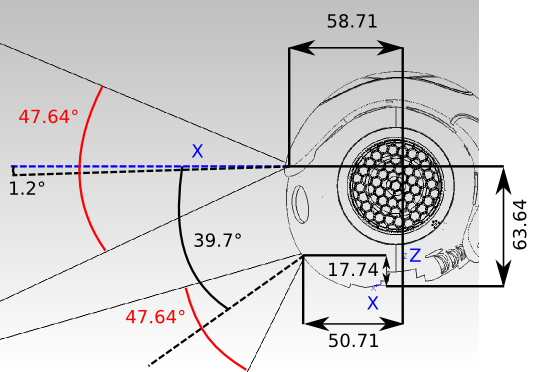
\includegraphics[width=0.8\textwidth]{nao_hardware_camera_lateral.png}
		\caption[Nao v5 camera positioning]{This figure shows camera positioning of Nao v5. Source: \cite{softbank_robotics_video_nodate}}
		\label{fig:naov5_cameras}
	\end{center}
\end{figure}
NAO V6 will be used officially in the upcoming RoboCup, thus it is also a priority to allow the calibration framework to be used with this platform. The cameras are upgraded to higher pixel density and they also feature auto focus which will be disabled due to being impossible to have a static intrinsic matrix for a given camera.

\subsubsection{Joint encoders}
\label{subsub:jointEncoders}

They feature magnetic incremental encoders with $0.1\degree$ precision. As mentioned previously, these sensors give feedback to closed loop controllers of the joints as well as let the software framework to calculate kinematic matrices \cite{softbank_robotics_joint_nodate}.

Based on experimental measurements in \cref{subsec:initial_joint_error}, it could be verified that these sensors are directly connected to output of joint actuators and their resolution is 12 bits (4096 values per $360\degree$ giving $0.0878\degree$ increments which is rounded off to $0.1\degree$ in documentation. This measurement also allowed to have an idea of possible noise of these sensors.

\subsubsection{Other Sensors}
The NAO also house other sensors such as IMU (Inertial Measurement Unit), microphones, sonar modules, FSR (Force Sensing Resistors). For this thesis, only the IMU is used in addition to Cameras and joint sensors.

\subsection{HULKs NAO framework}
This is the software framework developed by HULKs for NAO to play soccer in RoboCup SPL. It access robot's hardware through several software components provided by SoftBank Robotics. However it access cameras via a Linux kernel driver (Video For Linux - V4L2). Due to this difference and their cycle rates, two threads are employed for capturing sensor data; Vision (+ "brain" $\rightarrow$ perception \& behavior) and Motion. They cycle at 60Hz (30FPS per camera $x 2$) and 100Hz (rate set by NAOqi - the interface to access hardware)\todo{V6 updates}. Synchronization is done with a set of timestamped buffers and nearest (in temporal space) set of kinematic chain is selected for calibration purposes, therefore static poses are desirable for capturing images and joint values to get reliable readings due to limitations of this synchronizing method.

The framework also supports debugging and configuration via a debug tool "MATE" - also developed by HULKs.

In addition, this framework includes a module to compensate joint offset errors \todo{cite Code release?}. It offsets joints movement commands by the given value and it also compensate this value from sensor output, making the robot's perception unaware of induced offsets while correcting real-world shifts. Furthermore, camera calibration is possible with a module implemented for MATE.

Further information about HULKs NAO framework and tools is present in \cite{darshana_adikari_team_2017}.

\section{Camera calibration (extrinsic)}

Camera calibration is a well researched topic as it is a primary dependency for obtaining good results with camera systems. In this thesis, these standard methods \& tools for intrinsic calibration is employed, while extrinsic calibration is considered as well.

However, given that head yaw and pitch joints are close to camera origins and they are somewhat parallel to camera extrinsic parameters yaw and pitch respectively, they might cause a linear dependency or difficulty to observe together. Therefore it was decided not to calibrate camera extrinsic parameters at the same time as joints, but do separately with multiple rounds. This approach seem to be used by B-Human in their calibration procedure \cite{thomas_rofer_b-human_2018} and appear to be converging well.

\subsection{Method of HULKs}

The calibration process is based on the debug tool used by HULKs (MATE) as well as the HULKs NAO framework. In summary, the calibration is achieved by capturing images and kinematic chain with time synchronization to solve the following system of equations .with a non linear solver (Levenberg–Marquardt). The method of operation and usage is explained in \cite{darshana_adikari_team_2017}.

\subsection{Other RoboCup SPL teams}
\label{subsec:other_extrinsic_calib}
The team B-Human employs a method combined with joint calibration \cite{thomas_rofer_b-human_2018}. Nao-Team HTWK use center circle of a SPL soccer field as the calibration feature \cite{rico_tilgner_nto-team_2019}, their robots gather enough feature points in several poses to solve for calibration parameters. Berlin United also employs a similar approach but they do this with the robots in a sit down (un-stiffened) pose and they can use all line-features in a SPL field \cite{Berlin_United_TRR}.

\subsection{Calibration features}

For typical intrinsic calibration, a chessboard or similar pattern is used. For extrinsic calibration, the same can be used. In methods such as photogrammetry, a dense feature set is used to identify the relative position of the camera. 

However, one disadvantage with the classic chessboard pattern is that identification of the corners is a time consuming process and the existing methods relies on full visibility of the pattern in the image. As a solution for both limitations, ChAruco \cite{garrido-jurado_generation_2016}, \cite{romero-ramirez_speeded_2018} - a hybridization of the classic chessboard and AR markers to achieve fast detection and obtaining 3D points for partially visible patterns is employed via the implementation available in OpenCV library. \todo{cite}

\begin{center}
	\begin{figure}
		\def\svgwidth{\linewidth}
		\input{figures/calib_patterns.pdf_tex}
		\caption{(i) Chessboard, (ii) Aruco and (iii) ChAruco patterns with calibration features circled in red. AR (Augmented Reality) markers are used to quickly locate grid positioning and corner numbering and based on it approximate location (shown with green circles) of chessboard corners are found. Then it use sub-pixel optimization if specified to further optimize exact position of each chessboard corner. This approach is much faster than scanning whole image for a chessboard pattern according to \cite{romero-ramirez_speeded_2018}.}
		\label{fig:charuco}
	\end{figure}
\end{center}
\todo{check if CHESSBOARD PATTERN illustration is correct}

\section{Joint calibration}
This section discuss the fundamentals of joint errors, reasons for calibration and possible approaches.

\subsection{Joint error types}

Two major causes of joint positioning errors that affect overall end effector location are backlash and shifts of sensor or actuator causing joints to position with an offset. These causes joint actuators to point at physically incorrect locations although their positioning sensors precepts otherwise). Factors such as joint elasticity, looseness of mounting, worn bearings are not considered in the scope of this thesis.

\subsubsection{Backlash}
\label{subsec:backlash}
Backlash occurs due to necessary gap between gears (to avoid jamming) and wear occurred due to usage. Since output doesn't change when input is within this gap in a no load condition, it is also called "deadband". Even though the Nao appears to use gears aimed for low friction and low backlash, there is some amount of unavoidable backlash (Observed with Nao V5 refurbished, Nao V6 brand new) robots can be more than $1\degree$ and can be upto $\pm 5\degree$ according to \cite{kastner_automatic_2015} (which in return cite \cite{gouaillier_nao_2008} but it only mention a maximum of $3\degree$, yet personal observations confirm the former when Naos exhibit significant wear). Due to this unavoidable phenomena, a robot may not be in the position its sensors indicate and commanded to reach.

Figure \ref{fig:backlash} illustrate the effect of backlash while \cref{eq:output_backlash} models it with variables $D = deadband$, $i = input$, $o_i = \text{initial output}$. 

It should be noted that this model assumes initial velocity of output is zero whereas a complete model has to account forces/ torques applied upon the given joint's motion axis as that truly determines engagement direction or disengagement of input vs output. In addition, this model only cover simple case of backlash where gap is uniform throughout whole range of motion, no elastic deformations.

\begin{figure}
	\def\svgwidth{\linewidth}
	%LaTeX with PSTricks extensions
%%Creator: inkscape 0.91
%%Please note this file requires PSTricks extensions
\psset{xunit=.5pt,yunit=.5pt,runit=.5pt}
\begin{pspicture}(524.40944882,372.04724409)
{
\newrgbcolor{curcolor}{1 1 1}
\pscustom[linestyle=none,fillstyle=solid,fillcolor=curcolor]
{
\newpath
\moveto(137.62271404,213.2386539)
\curveto(137.62271404,213.17215935)(137.59937635,213.10683627)(137.55504664,213.04925029)
\lineto(137.11763775,213.2386539)
\closepath
}
}
{
\newrgbcolor{curcolor}{0 0 0}
\pscustom[linestyle=none,fillstyle=solid,fillcolor=curcolor]
{
\newpath
\moveto(142.670423,245.47755288)
\lineto(149.590423,249.47755288)
\lineto(149.590423,241.47755288)
\lineto(142.670423,245.47755288)
\closepath
}
}
{
\newrgbcolor{curcolor}{0 0 0}
\pscustom[linewidth=1,linecolor=curcolor]
{
\newpath
\moveto(142.670423,245.47755288)
\lineto(149.590423,249.47755288)
\lineto(149.590423,241.47755288)
\lineto(142.670423,245.47755288)
\closepath
}
}
{
\newrgbcolor{curcolor}{0.15294118 0.63137257 0.25882354}
\pscustom[linestyle=none,fillstyle=solid,fillcolor=curcolor]
{
\newpath
\moveto(148.75785,226.55394288)
\lineto(141.83785,222.55394288)
\lineto(141.83785,230.55394288)
\lineto(148.75785,226.55394288)
\closepath
}
}
{
\newrgbcolor{curcolor}{0.15294118 0.63137257 0.25882354}
\pscustom[linestyle=none,fillstyle=solid,fillcolor=curcolor]
{
\newpath
\moveto(148.75785,293.96400288)
\lineto(141.83785,289.96400288)
\lineto(141.83785,297.96400288)
\lineto(148.75785,293.96400288)
\closepath
}
}
{
\newrgbcolor{curcolor}{0.15294118 0.63137257 0.25882354}
\pscustom[linestyle=none,fillstyle=solid,fillcolor=curcolor]
{
\newpath
\moveto(127.64895011,260.25897288)
\lineto(131.16795434,262.29307938)
\lineto(131.16795434,258.22486639)
\lineto(127.64895011,260.25897288)
\closepath
}
}
{
\newrgbcolor{curcolor}{0.15294118 0.63137257 0.25882354}
\pscustom[linewidth=0.50852662,linecolor=curcolor]
{
\newpath
\moveto(127.64895011,260.25897288)
\lineto(131.16795434,262.29307938)
\lineto(131.16795434,258.22486639)
\lineto(127.64895011,260.25897288)
\closepath
}
}
{
\newrgbcolor{curcolor}{0 0 0}
\pscustom[linewidth=1,linecolor=curcolor]
{
\newpath
\moveto(118.130422,220.00000288)
\lineto(129.999714,220.00000288)
}
}
{
\newrgbcolor{curcolor}{0 0 0}
\pscustom[linewidth=1,linecolor=curcolor]
{
\newpath
\moveto(118.130706,280.00000288)
\lineto(129.999998,280.00000288)
}
}
{
\newrgbcolor{curcolor}{0 0 0}
\pscustom[linewidth=1,linecolor=curcolor]
{
\newpath
\moveto(118.130422,260.00000288)
\lineto(129.999714,260.00000288)
}
}
{
\newrgbcolor{curcolor}{0 0 0}
\pscustom[linewidth=1,linecolor=curcolor]
{
\newpath
\moveto(118.130706,300.00000288)
\lineto(129.999998,300.00000288)
}
}
{
\newrgbcolor{curcolor}{0 0 0}
\pscustom[linewidth=1,linecolor=curcolor]
{
\newpath
\moveto(118.130706,320.00000288)
\lineto(129.999998,320.00000288)
}
}
{
\newrgbcolor{curcolor}{0 0 0}
\pscustom[linewidth=1,linecolor=curcolor]
{
\newpath
\moveto(118.130422,240.00000288)
\lineto(129.999714,240.00000288)
}
}
{
\newrgbcolor{curcolor}{0 0 0}
\pscustom[linewidth=1,linecolor=curcolor]
{
\newpath
\moveto(118.130422,200.00000288)
\lineto(129.999714,200.00000288)
}
}
{
\newrgbcolor{curcolor}{0 0 0}
\pscustom[linestyle=none,fillstyle=solid,fillcolor=curcolor]
{
\newpath
\moveto(97.75667583,319.49951435)
\lineto(100.38851177,319.49951435)
\lineto(100.38851177,318.6987331)
\lineto(97.75667583,318.6987331)
\lineto(97.75667583,319.49951435)
\closepath
}
}
{
\newrgbcolor{curcolor}{0 0 0}
\pscustom[linestyle=none,fillstyle=solid,fillcolor=curcolor]
{
\newpath
\moveto(104.93929302,320.29052997)
\curveto(105.41129823,320.18961851)(105.77913677,319.97965758)(106.04280864,319.66064716)
\curveto(106.30973573,319.34163674)(106.44319927,318.94775653)(106.44319927,318.47900653)
\curveto(106.44319927,317.75960549)(106.19580344,317.20296487)(105.70101177,316.80908466)
\curveto(105.2062201,316.41520445)(104.5030951,316.21826435)(103.59163677,316.21826435)
\curveto(103.28564719,316.21826435)(102.96989198,316.24918883)(102.64437114,316.31103778)
\curveto(102.32210552,316.36963153)(101.98844667,316.45914976)(101.64339458,316.57959247)
\lineto(101.64339458,317.53174091)
\curveto(101.91683208,317.3722357)(102.21631125,317.25179299)(102.54183208,317.17041278)
\curveto(102.86735292,317.08903258)(103.20752219,317.04834247)(103.56233989,317.04834247)
\curveto(104.18082948,317.04834247)(104.65120708,317.17041278)(104.97347271,317.41455341)
\curveto(105.29899354,317.65869403)(105.46175396,318.01351174)(105.46175396,318.47900653)
\curveto(105.46175396,318.90869403)(105.31038677,319.24398049)(105.00765239,319.48486591)
\curveto(104.70817323,319.72900653)(104.28987896,319.85107685)(103.75276958,319.85107685)
\lineto(102.90316021,319.85107685)
\lineto(102.90316021,320.66162372)
\lineto(103.79183208,320.66162372)
\curveto(104.27685812,320.66162372)(104.64795187,320.75765237)(104.90511333,320.94970966)
\curveto(105.16227479,321.14502216)(105.29085552,321.42497008)(105.29085552,321.78955341)
\curveto(105.29085552,322.16390237)(105.15739198,322.4503607)(104.89046489,322.64892841)
\curveto(104.62679302,322.85075133)(104.24756125,322.95166278)(103.75276958,322.95166278)
\curveto(103.48258729,322.95166278)(103.19287375,322.92236591)(102.88362896,322.86377216)
\curveto(102.57438417,322.80517841)(102.23421489,322.71403258)(101.86312114,322.59033466)
\lineto(101.86312114,323.46924091)
\curveto(102.2374701,323.57340758)(102.587405,323.65153258)(102.91292583,323.70361591)
\curveto(103.24170187,323.75569924)(103.55094667,323.78174091)(103.84066021,323.78174091)
\curveto(104.58935812,323.78174091)(105.18180604,323.61084247)(105.61800396,323.2690456)
\curveto(106.05420187,322.93050393)(106.27230083,322.47151956)(106.27230083,321.89209247)
\curveto(106.27230083,321.48844664)(106.15674094,321.14664976)(105.92562114,320.86670185)
\curveto(105.69450135,320.59000914)(105.36572531,320.39795185)(104.93929302,320.29052997)
\closepath
}
}
{
\newrgbcolor{curcolor}{0 0 0}
\pscustom[linestyle=none,fillstyle=solid,fillcolor=curcolor]
{
\newpath
\moveto(108.31819927,317.60010028)
\lineto(109.34847271,317.60010028)
\lineto(109.34847271,316.35986591)
\lineto(108.31819927,316.35986591)
\lineto(108.31819927,317.60010028)
\closepath
}
}
{
\newrgbcolor{curcolor}{0 0 0}
\pscustom[linestyle=none,fillstyle=solid,fillcolor=curcolor]
{
\newpath
\moveto(113.61116802,323.00049091)
\curveto(113.10335552,323.00049091)(112.72086854,322.74983987)(112.46370708,322.24853778)
\curveto(112.20980083,321.75049091)(112.08284771,321.00016539)(112.08284771,319.99756122)
\curveto(112.08284771,318.99821226)(112.20980083,318.24788674)(112.46370708,317.74658466)
\curveto(112.72086854,317.24853778)(113.10335552,316.99951435)(113.61116802,316.99951435)
\curveto(114.12223573,316.99951435)(114.50472271,317.24853778)(114.75862896,317.74658466)
\curveto(115.01579042,318.24788674)(115.14437114,318.99821226)(115.14437114,319.99756122)
\curveto(115.14437114,321.00016539)(115.01579042,321.75049091)(114.75862896,322.24853778)
\curveto(114.50472271,322.74983987)(114.12223573,323.00049091)(113.61116802,323.00049091)
\closepath
\moveto(113.61116802,323.78174091)
\curveto(114.42822531,323.78174091)(115.05159771,323.45784768)(115.48128521,322.81006122)
\curveto(115.91422792,322.16552997)(116.13069927,321.22802997)(116.13069927,319.99756122)
\curveto(116.13069927,318.77034768)(115.91422792,317.83284768)(115.48128521,317.18506122)
\curveto(115.05159771,316.54052997)(114.42822531,316.21826435)(113.61116802,316.21826435)
\curveto(112.79411073,316.21826435)(112.16911073,316.54052997)(111.73616802,317.18506122)
\curveto(111.30648052,317.83284768)(111.09163677,318.77034768)(111.09163677,319.99756122)
\curveto(111.09163677,321.22802997)(111.30648052,322.16552997)(111.73616802,322.81006122)
\curveto(112.16911073,323.45784768)(112.79411073,323.78174091)(113.61116802,323.78174091)
\closepath
}
}
{
\newrgbcolor{curcolor}{0 0 0}
\pscustom[linestyle=none,fillstyle=solid,fillcolor=curcolor]
{
\newpath
\moveto(97.75667583,299.49951435)
\lineto(100.38851177,299.49951435)
\lineto(100.38851177,298.6987331)
\lineto(97.75667583,298.6987331)
\lineto(97.75667583,299.49951435)
\closepath
}
}
{
\newrgbcolor{curcolor}{0 0 0}
\pscustom[linestyle=none,fillstyle=solid,fillcolor=curcolor]
{
\newpath
\moveto(102.80062114,297.18994403)
\lineto(106.24300396,297.18994403)
\lineto(106.24300396,296.35986591)
\lineto(101.61409771,296.35986591)
\lineto(101.61409771,297.18994403)
\curveto(101.98844667,297.57731383)(102.49788677,298.09651956)(103.14241802,298.74756122)
\curveto(103.79020448,299.4018581)(104.19710552,299.82340758)(104.36312114,300.01220966)
\curveto(104.67887635,300.36702737)(104.89860292,300.66650653)(105.02230083,300.91064716)
\curveto(105.14925396,301.15804299)(105.21273052,301.40055601)(105.21273052,301.63818622)
\curveto(105.21273052,302.02555601)(105.07601177,302.34131122)(104.80257427,302.58545185)
\curveto(104.53239198,302.82959247)(104.17920187,302.95166278)(103.74300396,302.95166278)
\curveto(103.43375917,302.95166278)(103.10661073,302.89795185)(102.76155864,302.79052997)
\curveto(102.41976177,302.6831081)(102.05355083,302.52034768)(101.66292583,302.30224872)
\lineto(101.66292583,303.29834247)
\curveto(102.06006125,303.45784768)(102.431155,303.57829039)(102.77620708,303.6596706)
\curveto(103.12125917,303.74105081)(103.43701437,303.78174091)(103.72347271,303.78174091)
\curveto(104.47868104,303.78174091)(105.08089458,303.59293883)(105.53011333,303.21533466)
\curveto(105.97933208,302.83773049)(106.20394146,302.3331732)(106.20394146,301.70166278)
\curveto(106.20394146,301.40218362)(106.14697531,301.11735289)(106.03304302,300.8471706)
\curveto(105.92236594,300.58024351)(105.71891542,300.26448831)(105.42269146,299.89990497)
\curveto(105.34131125,299.80550393)(105.08252219,299.53206643)(104.64632427,299.07959247)
\curveto(104.21012635,298.63037372)(103.59489198,298.00049091)(102.80062114,297.18994403)
\closepath
}
}
{
\newrgbcolor{curcolor}{0 0 0}
\pscustom[linestyle=none,fillstyle=solid,fillcolor=curcolor]
{
\newpath
\moveto(108.31819927,297.60010028)
\lineto(109.34847271,297.60010028)
\lineto(109.34847271,296.35986591)
\lineto(108.31819927,296.35986591)
\lineto(108.31819927,297.60010028)
\closepath
}
}
{
\newrgbcolor{curcolor}{0 0 0}
\pscustom[linestyle=none,fillstyle=solid,fillcolor=curcolor]
{
\newpath
\moveto(113.61116802,303.00049091)
\curveto(113.10335552,303.00049091)(112.72086854,302.74983987)(112.46370708,302.24853778)
\curveto(112.20980083,301.75049091)(112.08284771,301.00016539)(112.08284771,299.99756122)
\curveto(112.08284771,298.99821226)(112.20980083,298.24788674)(112.46370708,297.74658466)
\curveto(112.72086854,297.24853778)(113.10335552,296.99951435)(113.61116802,296.99951435)
\curveto(114.12223573,296.99951435)(114.50472271,297.24853778)(114.75862896,297.74658466)
\curveto(115.01579042,298.24788674)(115.14437114,298.99821226)(115.14437114,299.99756122)
\curveto(115.14437114,301.00016539)(115.01579042,301.75049091)(114.75862896,302.24853778)
\curveto(114.50472271,302.74983987)(114.12223573,303.00049091)(113.61116802,303.00049091)
\closepath
\moveto(113.61116802,303.78174091)
\curveto(114.42822531,303.78174091)(115.05159771,303.45784768)(115.48128521,302.81006122)
\curveto(115.91422792,302.16552997)(116.13069927,301.22802997)(116.13069927,299.99756122)
\curveto(116.13069927,298.77034768)(115.91422792,297.83284768)(115.48128521,297.18506122)
\curveto(115.05159771,296.54052997)(114.42822531,296.21826435)(113.61116802,296.21826435)
\curveto(112.79411073,296.21826435)(112.16911073,296.54052997)(111.73616802,297.18506122)
\curveto(111.30648052,297.83284768)(111.09163677,298.77034768)(111.09163677,299.99756122)
\curveto(111.09163677,301.22802997)(111.30648052,302.16552997)(111.73616802,302.81006122)
\curveto(112.16911073,303.45784768)(112.79411073,303.78174091)(113.61116802,303.78174091)
\closepath
}
}
{
\newrgbcolor{curcolor}{0 0 0}
\pscustom[linestyle=none,fillstyle=solid,fillcolor=curcolor]
{
\newpath
\moveto(97.75667583,279.49951816)
\lineto(100.38851177,279.49951816)
\lineto(100.38851177,278.69873691)
\lineto(97.75667583,278.69873691)
\lineto(97.75667583,279.49951816)
\closepath
}
}
{
\newrgbcolor{curcolor}{0 0 0}
\pscustom[linestyle=none,fillstyle=solid,fillcolor=curcolor]
{
\newpath
\moveto(102.12191021,277.18994785)
\lineto(103.73323833,277.18994785)
\lineto(103.73323833,282.75147129)
\lineto(101.98030864,282.39990879)
\lineto(101.98030864,283.29834629)
\lineto(103.72347271,283.64990879)
\lineto(104.70980083,283.64990879)
\lineto(104.70980083,277.18994785)
\lineto(106.32112896,277.18994785)
\lineto(106.32112896,276.35986972)
\lineto(102.12191021,276.35986972)
\lineto(102.12191021,277.18994785)
\closepath
}
}
{
\newrgbcolor{curcolor}{0 0 0}
\pscustom[linestyle=none,fillstyle=solid,fillcolor=curcolor]
{
\newpath
\moveto(108.31819927,277.6001041)
\lineto(109.34847271,277.6001041)
\lineto(109.34847271,276.35986972)
\lineto(108.31819927,276.35986972)
\lineto(108.31819927,277.6001041)
\closepath
}
}
{
\newrgbcolor{curcolor}{0 0 0}
\pscustom[linestyle=none,fillstyle=solid,fillcolor=curcolor]
{
\newpath
\moveto(113.61116802,283.00049472)
\curveto(113.10335552,283.00049472)(112.72086854,282.74984368)(112.46370708,282.2485416)
\curveto(112.20980083,281.75049472)(112.08284771,281.0001692)(112.08284771,279.99756504)
\curveto(112.08284771,278.99821608)(112.20980083,278.24789056)(112.46370708,277.74658847)
\curveto(112.72086854,277.2485416)(113.10335552,276.99951816)(113.61116802,276.99951816)
\curveto(114.12223573,276.99951816)(114.50472271,277.2485416)(114.75862896,277.74658847)
\curveto(115.01579042,278.24789056)(115.14437114,278.99821608)(115.14437114,279.99756504)
\curveto(115.14437114,281.0001692)(115.01579042,281.75049472)(114.75862896,282.2485416)
\curveto(114.50472271,282.74984368)(114.12223573,283.00049472)(113.61116802,283.00049472)
\closepath
\moveto(113.61116802,283.78174472)
\curveto(114.42822531,283.78174472)(115.05159771,283.4578515)(115.48128521,282.81006504)
\curveto(115.91422792,282.16553379)(116.13069927,281.22803379)(116.13069927,279.99756504)
\curveto(116.13069927,278.7703515)(115.91422792,277.8328515)(115.48128521,277.18506504)
\curveto(115.05159771,276.54053379)(114.42822531,276.21826816)(113.61116802,276.21826816)
\curveto(112.79411073,276.21826816)(112.16911073,276.54053379)(111.73616802,277.18506504)
\curveto(111.30648052,277.8328515)(111.09163677,278.7703515)(111.09163677,279.99756504)
\curveto(111.09163677,281.22803379)(111.30648052,282.16553379)(111.73616802,282.81006504)
\curveto(112.16911073,283.4578515)(112.79411073,283.78174472)(113.61116802,283.78174472)
\closepath
}
}
{
\newrgbcolor{curcolor}{0 0 0}
\pscustom[linestyle=none,fillstyle=solid,fillcolor=curcolor]
{
\newpath
\moveto(104.06011211,263.00049472)
\curveto(103.55229961,263.00049472)(103.16981263,262.74984368)(102.91265117,262.2485416)
\curveto(102.65874492,261.75049472)(102.5317918,261.0001692)(102.5317918,259.99756504)
\curveto(102.5317918,258.99821608)(102.65874492,258.24789056)(102.91265117,257.74658847)
\curveto(103.16981263,257.2485416)(103.55229961,256.99951816)(104.06011211,256.99951816)
\curveto(104.57117982,256.99951816)(104.9536668,257.2485416)(105.20757305,257.74658847)
\curveto(105.46473451,258.24789056)(105.59331524,258.99821608)(105.59331524,259.99756504)
\curveto(105.59331524,261.0001692)(105.46473451,261.75049472)(105.20757305,262.2485416)
\curveto(104.9536668,262.74984368)(104.57117982,263.00049472)(104.06011211,263.00049472)
\closepath
\moveto(104.06011211,263.78174472)
\curveto(104.8771694,263.78174472)(105.5005418,263.4578515)(105.9302293,262.81006504)
\curveto(106.36317201,262.16553379)(106.57964336,261.22803379)(106.57964336,259.99756504)
\curveto(106.57964336,258.7703515)(106.36317201,257.8328515)(105.9302293,257.18506504)
\curveto(105.5005418,256.54053379)(104.8771694,256.21826816)(104.06011211,256.21826816)
\curveto(103.24305482,256.21826816)(102.61805482,256.54053379)(102.18511211,257.18506504)
\curveto(101.75542461,257.8328515)(101.54058086,258.7703515)(101.54058086,259.99756504)
\curveto(101.54058086,261.22803379)(101.75542461,262.16553379)(102.18511211,262.81006504)
\curveto(102.61805482,263.4578515)(103.24305482,263.78174472)(104.06011211,263.78174472)
\closepath
}
}
{
\newrgbcolor{curcolor}{0 0 0}
\pscustom[linestyle=none,fillstyle=solid,fillcolor=curcolor]
{
\newpath
\moveto(108.31792461,257.6001041)
\lineto(109.34819805,257.6001041)
\lineto(109.34819805,256.35986972)
\lineto(108.31792461,256.35986972)
\lineto(108.31792461,257.6001041)
\closepath
}
}
{
\newrgbcolor{curcolor}{0 0 0}
\pscustom[linestyle=none,fillstyle=solid,fillcolor=curcolor]
{
\newpath
\moveto(113.61089336,263.00049472)
\curveto(113.10308086,263.00049472)(112.72059388,262.74984368)(112.46343242,262.2485416)
\curveto(112.20952617,261.75049472)(112.08257305,261.0001692)(112.08257305,259.99756504)
\curveto(112.08257305,258.99821608)(112.20952617,258.24789056)(112.46343242,257.74658847)
\curveto(112.72059388,257.2485416)(113.10308086,256.99951816)(113.61089336,256.99951816)
\curveto(114.12196107,256.99951816)(114.50444805,257.2485416)(114.7583543,257.74658847)
\curveto(115.01551576,258.24789056)(115.14409649,258.99821608)(115.14409649,259.99756504)
\curveto(115.14409649,261.0001692)(115.01551576,261.75049472)(114.7583543,262.2485416)
\curveto(114.50444805,262.74984368)(114.12196107,263.00049472)(113.61089336,263.00049472)
\closepath
\moveto(113.61089336,263.78174472)
\curveto(114.42795065,263.78174472)(115.05132305,263.4578515)(115.48101055,262.81006504)
\curveto(115.91395326,262.16553379)(116.13042461,261.22803379)(116.13042461,259.99756504)
\curveto(116.13042461,258.7703515)(115.91395326,257.8328515)(115.48101055,257.18506504)
\curveto(115.05132305,256.54053379)(114.42795065,256.21826816)(113.61089336,256.21826816)
\curveto(112.79383607,256.21826816)(112.16883607,256.54053379)(111.73589336,257.18506504)
\curveto(111.30620586,257.8328515)(111.09136211,258.7703515)(111.09136211,259.99756504)
\curveto(111.09136211,261.22803379)(111.30620586,262.16553379)(111.73589336,262.81006504)
\curveto(112.16883607,263.4578515)(112.79383607,263.78174472)(113.61089336,263.78174472)
\closepath
}
}
{
\newrgbcolor{curcolor}{0 0 0}
\pscustom[linestyle=none,fillstyle=solid,fillcolor=curcolor]
{
\newpath
\moveto(102.12163555,237.18994785)
\lineto(103.73296367,237.18994785)
\lineto(103.73296367,242.75147129)
\lineto(101.98003399,242.39990879)
\lineto(101.98003399,243.29834629)
\lineto(103.72319805,243.64990879)
\lineto(104.70952617,243.64990879)
\lineto(104.70952617,237.18994785)
\lineto(106.3208543,237.18994785)
\lineto(106.3208543,236.35986972)
\lineto(102.12163555,236.35986972)
\lineto(102.12163555,237.18994785)
\closepath
}
}
{
\newrgbcolor{curcolor}{0 0 0}
\pscustom[linestyle=none,fillstyle=solid,fillcolor=curcolor]
{
\newpath
\moveto(108.31792461,237.6001041)
\lineto(109.34819805,237.6001041)
\lineto(109.34819805,236.35986972)
\lineto(108.31792461,236.35986972)
\lineto(108.31792461,237.6001041)
\closepath
}
}
{
\newrgbcolor{curcolor}{0 0 0}
\pscustom[linestyle=none,fillstyle=solid,fillcolor=curcolor]
{
\newpath
\moveto(113.61089336,243.00049472)
\curveto(113.10308086,243.00049472)(112.72059388,242.74984368)(112.46343242,242.2485416)
\curveto(112.20952617,241.75049472)(112.08257305,241.0001692)(112.08257305,239.99756504)
\curveto(112.08257305,238.99821608)(112.20952617,238.24789056)(112.46343242,237.74658847)
\curveto(112.72059388,237.2485416)(113.10308086,236.99951816)(113.61089336,236.99951816)
\curveto(114.12196107,236.99951816)(114.50444805,237.2485416)(114.7583543,237.74658847)
\curveto(115.01551576,238.24789056)(115.14409649,238.99821608)(115.14409649,239.99756504)
\curveto(115.14409649,241.0001692)(115.01551576,241.75049472)(114.7583543,242.2485416)
\curveto(114.50444805,242.74984368)(114.12196107,243.00049472)(113.61089336,243.00049472)
\closepath
\moveto(113.61089336,243.78174472)
\curveto(114.42795065,243.78174472)(115.05132305,243.4578515)(115.48101055,242.81006504)
\curveto(115.91395326,242.16553379)(116.13042461,241.22803379)(116.13042461,239.99756504)
\curveto(116.13042461,238.7703515)(115.91395326,237.8328515)(115.48101055,237.18506504)
\curveto(115.05132305,236.54053379)(114.42795065,236.21826816)(113.61089336,236.21826816)
\curveto(112.79383607,236.21826816)(112.16883607,236.54053379)(111.73589336,237.18506504)
\curveto(111.30620586,237.8328515)(111.09136211,238.7703515)(111.09136211,239.99756504)
\curveto(111.09136211,241.22803379)(111.30620586,242.16553379)(111.73589336,242.81006504)
\curveto(112.16883607,243.4578515)(112.79383607,243.78174472)(113.61089336,243.78174472)
\closepath
}
}
{
\newrgbcolor{curcolor}{0 0 0}
\pscustom[linestyle=none,fillstyle=solid,fillcolor=curcolor]
{
\newpath
\moveto(102.80034649,217.18994785)
\lineto(106.2427293,217.18994785)
\lineto(106.2427293,216.35986972)
\lineto(101.61382305,216.35986972)
\lineto(101.61382305,217.18994785)
\curveto(101.98817201,217.57731764)(102.49761211,218.09652337)(103.14214336,218.74756504)
\curveto(103.78992982,219.40186191)(104.19683086,219.82341139)(104.36284649,220.01221347)
\curveto(104.67860169,220.36703118)(104.89832826,220.66651035)(105.02202617,220.91065097)
\curveto(105.1489793,221.15804681)(105.21245586,221.40055983)(105.21245586,221.63819004)
\curveto(105.21245586,222.02555983)(105.07573711,222.34131504)(104.80229961,222.58545566)
\curveto(104.53211732,222.82959629)(104.17892722,222.9516666)(103.7427293,222.9516666)
\curveto(103.43348451,222.9516666)(103.10633607,222.89795566)(102.76128399,222.79053379)
\curveto(102.41948711,222.68311191)(102.05327617,222.5203515)(101.66265117,222.30225254)
\lineto(101.66265117,223.29834629)
\curveto(102.05978659,223.4578515)(102.43088034,223.5782942)(102.77593242,223.65967441)
\curveto(103.12098451,223.74105462)(103.43673972,223.78174472)(103.72319805,223.78174472)
\curveto(104.47840638,223.78174472)(105.08061992,223.59294264)(105.52983867,223.21533847)
\curveto(105.97905742,222.83773431)(106.2036668,222.33317702)(106.2036668,221.7016666)
\curveto(106.2036668,221.40218743)(106.14670065,221.1173567)(106.03276836,220.84717441)
\curveto(105.92209128,220.58024733)(105.71864076,220.26449212)(105.4224168,219.89990879)
\curveto(105.34103659,219.80550775)(105.08224753,219.53207025)(104.64604961,219.07959629)
\curveto(104.20985169,218.63037754)(103.59461732,218.00049472)(102.80034649,217.18994785)
\closepath
}
}
{
\newrgbcolor{curcolor}{0 0 0}
\pscustom[linestyle=none,fillstyle=solid,fillcolor=curcolor]
{
\newpath
\moveto(108.31792461,217.6001041)
\lineto(109.34819805,217.6001041)
\lineto(109.34819805,216.35986972)
\lineto(108.31792461,216.35986972)
\lineto(108.31792461,217.6001041)
\closepath
}
}
{
\newrgbcolor{curcolor}{0 0 0}
\pscustom[linestyle=none,fillstyle=solid,fillcolor=curcolor]
{
\newpath
\moveto(113.61089336,223.00049472)
\curveto(113.10308086,223.00049472)(112.72059388,222.74984368)(112.46343242,222.2485416)
\curveto(112.20952617,221.75049472)(112.08257305,221.0001692)(112.08257305,219.99756504)
\curveto(112.08257305,218.99821608)(112.20952617,218.24789056)(112.46343242,217.74658847)
\curveto(112.72059388,217.2485416)(113.10308086,216.99951816)(113.61089336,216.99951816)
\curveto(114.12196107,216.99951816)(114.50444805,217.2485416)(114.7583543,217.74658847)
\curveto(115.01551576,218.24789056)(115.14409649,218.99821608)(115.14409649,219.99756504)
\curveto(115.14409649,221.0001692)(115.01551576,221.75049472)(114.7583543,222.2485416)
\curveto(114.50444805,222.74984368)(114.12196107,223.00049472)(113.61089336,223.00049472)
\closepath
\moveto(113.61089336,223.78174472)
\curveto(114.42795065,223.78174472)(115.05132305,223.4578515)(115.48101055,222.81006504)
\curveto(115.91395326,222.16553379)(116.13042461,221.22803379)(116.13042461,219.99756504)
\curveto(116.13042461,218.7703515)(115.91395326,217.8328515)(115.48101055,217.18506504)
\curveto(115.05132305,216.54053379)(114.42795065,216.21826816)(113.61089336,216.21826816)
\curveto(112.79383607,216.21826816)(112.16883607,216.54053379)(111.73589336,217.18506504)
\curveto(111.30620586,217.8328515)(111.09136211,218.7703515)(111.09136211,219.99756504)
\curveto(111.09136211,221.22803379)(111.30620586,222.16553379)(111.73589336,222.81006504)
\curveto(112.16883607,223.4578515)(112.79383607,223.78174472)(113.61089336,223.78174472)
\closepath
}
}
{
\newrgbcolor{curcolor}{0 0 0}
\pscustom[linestyle=none,fillstyle=solid,fillcolor=curcolor]
{
\newpath
\moveto(104.93901836,200.29053379)
\curveto(105.41102357,200.18962233)(105.77886211,199.97966139)(106.04253399,199.66065097)
\curveto(106.30946107,199.34164056)(106.44292461,198.94776035)(106.44292461,198.47901035)
\curveto(106.44292461,197.75960931)(106.19552878,197.20296868)(105.70073711,196.80908847)
\curveto(105.20594544,196.41520827)(104.50282044,196.21826816)(103.59136211,196.21826816)
\curveto(103.28537253,196.21826816)(102.96961732,196.24919264)(102.64409649,196.3110416)
\curveto(102.32183086,196.36963535)(101.98817201,196.45915358)(101.64311992,196.57959629)
\lineto(101.64311992,197.53174472)
\curveto(101.91655742,197.37223952)(102.21603659,197.25179681)(102.54155742,197.1704166)
\curveto(102.86707826,197.08903639)(103.20724753,197.04834629)(103.56206524,197.04834629)
\curveto(104.18055482,197.04834629)(104.65093242,197.1704166)(104.97319805,197.41455722)
\curveto(105.29871888,197.65869785)(105.4614793,198.01351556)(105.4614793,198.47901035)
\curveto(105.4614793,198.90869785)(105.31011211,199.24398431)(105.00737774,199.48486972)
\curveto(104.70789857,199.72901035)(104.2896043,199.85108066)(103.75249492,199.85108066)
\lineto(102.90288555,199.85108066)
\lineto(102.90288555,200.66162754)
\lineto(103.79155742,200.66162754)
\curveto(104.27658347,200.66162754)(104.64767722,200.75765618)(104.90483867,200.94971347)
\curveto(105.16200013,201.14502597)(105.29058086,201.42497389)(105.29058086,201.78955722)
\curveto(105.29058086,202.16390618)(105.15711732,202.45036452)(104.89019024,202.64893222)
\curveto(104.62651836,202.85075514)(104.24728659,202.9516666)(103.75249492,202.9516666)
\curveto(103.48231263,202.9516666)(103.19259909,202.92236972)(102.8833543,202.86377597)
\curveto(102.57410951,202.80518222)(102.23394024,202.71403639)(101.86284649,202.59033847)
\lineto(101.86284649,203.46924472)
\curveto(102.23719544,203.57341139)(102.58713034,203.65153639)(102.91265117,203.70361972)
\curveto(103.24142722,203.75570306)(103.55067201,203.78174472)(103.84038555,203.78174472)
\curveto(104.58908347,203.78174472)(105.18153138,203.61084629)(105.6177293,203.26904941)
\curveto(106.05392722,202.93050775)(106.27202617,202.47152337)(106.27202617,201.89209629)
\curveto(106.27202617,201.48845045)(106.15646628,201.14665358)(105.92534649,200.86670566)
\curveto(105.69422669,200.59001295)(105.36545065,200.39795566)(104.93901836,200.29053379)
\closepath
}
}
{
\newrgbcolor{curcolor}{0 0 0}
\pscustom[linestyle=none,fillstyle=solid,fillcolor=curcolor]
{
\newpath
\moveto(108.31792461,197.6001041)
\lineto(109.34819805,197.6001041)
\lineto(109.34819805,196.35986972)
\lineto(108.31792461,196.35986972)
\lineto(108.31792461,197.6001041)
\closepath
}
}
{
\newrgbcolor{curcolor}{0 0 0}
\pscustom[linestyle=none,fillstyle=solid,fillcolor=curcolor]
{
\newpath
\moveto(113.61089336,203.00049472)
\curveto(113.10308086,203.00049472)(112.72059388,202.74984368)(112.46343242,202.2485416)
\curveto(112.20952617,201.75049472)(112.08257305,201.0001692)(112.08257305,199.99756504)
\curveto(112.08257305,198.99821608)(112.20952617,198.24789056)(112.46343242,197.74658847)
\curveto(112.72059388,197.2485416)(113.10308086,196.99951816)(113.61089336,196.99951816)
\curveto(114.12196107,196.99951816)(114.50444805,197.2485416)(114.7583543,197.74658847)
\curveto(115.01551576,198.24789056)(115.14409649,198.99821608)(115.14409649,199.99756504)
\curveto(115.14409649,201.0001692)(115.01551576,201.75049472)(114.7583543,202.2485416)
\curveto(114.50444805,202.74984368)(114.12196107,203.00049472)(113.61089336,203.00049472)
\closepath
\moveto(113.61089336,203.78174472)
\curveto(114.42795065,203.78174472)(115.05132305,203.4578515)(115.48101055,202.81006504)
\curveto(115.91395326,202.16553379)(116.13042461,201.22803379)(116.13042461,199.99756504)
\curveto(116.13042461,198.7703515)(115.91395326,197.8328515)(115.48101055,197.18506504)
\curveto(115.05132305,196.54053379)(114.42795065,196.21826816)(113.61089336,196.21826816)
\curveto(112.79383607,196.21826816)(112.16883607,196.54053379)(111.73589336,197.18506504)
\curveto(111.30620586,197.8328515)(111.09136211,198.7703515)(111.09136211,199.99756504)
\curveto(111.09136211,201.22803379)(111.30620586,202.16553379)(111.73589336,202.81006504)
\curveto(112.16883607,203.4578515)(112.79383607,203.78174472)(113.61089336,203.78174472)
\closepath
}
}
{
\newrgbcolor{curcolor}{0 0 0}
\pscustom[linestyle=none,fillstyle=solid,fillcolor=curcolor]
{
\newpath
\moveto(276.042293,230.29497288)
\lineto(282.962293,234.29497288)
\lineto(282.962293,226.29497288)
\lineto(276.042293,230.29497288)
\closepath
}
}
{
\newrgbcolor{curcolor}{0 0 0}
\pscustom[linewidth=1,linecolor=curcolor]
{
\newpath
\moveto(276.042293,230.29497288)
\lineto(282.962293,234.29497288)
\lineto(282.962293,226.29497288)
\lineto(276.042293,230.29497288)
\closepath
}
}
{
\newrgbcolor{curcolor}{0.15294118 0.63137257 0.25882354}
\pscustom[linestyle=none,fillstyle=solid,fillcolor=curcolor]
{
\newpath
\moveto(282.002832,226.29497288)
\lineto(275.082832,222.29497288)
\lineto(275.082832,230.29497288)
\lineto(282.002832,226.29497288)
\closepath
}
}
{
\newrgbcolor{curcolor}{0.15294118 0.63137257 0.25882354}
\pscustom[linestyle=none,fillstyle=solid,fillcolor=curcolor]
{
\newpath
\moveto(282.002832,293.70503288)
\lineto(275.082832,289.70503288)
\lineto(275.082832,297.70503288)
\lineto(282.002832,293.70503288)
\closepath
}
}
{
\newrgbcolor{curcolor}{0.15294118 0.63137257 0.25882354}
\pscustom[linestyle=none,fillstyle=solid,fillcolor=curcolor]
{
\newpath
\moveto(260.89393211,260.00000288)
\lineto(264.41293634,262.03410938)
\lineto(264.41293634,257.96589639)
\lineto(260.89393211,260.00000288)
\closepath
}
}
{
\newrgbcolor{curcolor}{0.15294118 0.63137257 0.25882354}
\pscustom[linewidth=0.50852662,linecolor=curcolor]
{
\newpath
\moveto(260.89393211,260.00000288)
\lineto(264.41293634,262.03410938)
\lineto(264.41293634,257.96589639)
\lineto(260.89393211,260.00000288)
\closepath
}
}
{
\newrgbcolor{curcolor}{0 0 0}
\pscustom[linewidth=1,linecolor=curcolor]
{
\newpath
\moveto(249.999716,220.00000288)
\lineto(261.869008,220.00000288)
}
}
{
\newrgbcolor{curcolor}{0 0 0}
\pscustom[linewidth=1,linecolor=curcolor]
{
\newpath
\moveto(250,280.00000288)
\lineto(261.869292,280.00000288)
}
}
{
\newrgbcolor{curcolor}{0 0 0}
\pscustom[linewidth=1,linecolor=curcolor]
{
\newpath
\moveto(249.999716,260.00000288)
\lineto(261.869008,260.00000288)
}
}
{
\newrgbcolor{curcolor}{0 0 0}
\pscustom[linewidth=1,linecolor=curcolor]
{
\newpath
\moveto(250,300.00000288)
\lineto(261.869292,300.00000288)
}
}
{
\newrgbcolor{curcolor}{0 0 0}
\pscustom[linewidth=1,linecolor=curcolor]
{
\newpath
\moveto(250,320.00000288)
\lineto(261.869292,320.00000288)
}
}
{
\newrgbcolor{curcolor}{0 0 0}
\pscustom[linewidth=1,linecolor=curcolor]
{
\newpath
\moveto(249.999716,240.00000288)
\lineto(261.869008,240.00000288)
}
}
{
\newrgbcolor{curcolor}{0 0 0}
\pscustom[linewidth=1,linecolor=curcolor]
{
\newpath
\moveto(249.999716,200.00000288)
\lineto(261.869008,200.00000288)
}
}
{
\newrgbcolor{curcolor}{0 0 0}
\pscustom[linestyle=none,fillstyle=solid,fillcolor=curcolor]
{
\newpath
\moveto(229.62596983,319.49951435)
\lineto(232.25780577,319.49951435)
\lineto(232.25780577,318.6987331)
\lineto(229.62596983,318.6987331)
\lineto(229.62596983,319.49951435)
\closepath
}
}
{
\newrgbcolor{curcolor}{0 0 0}
\pscustom[linestyle=none,fillstyle=solid,fillcolor=curcolor]
{
\newpath
\moveto(236.80858702,320.29052997)
\curveto(237.28059223,320.18961851)(237.64843077,319.97965758)(237.91210264,319.66064716)
\curveto(238.17902973,319.34163674)(238.31249327,318.94775653)(238.31249327,318.47900653)
\curveto(238.31249327,317.75960549)(238.06509744,317.20296487)(237.57030577,316.80908466)
\curveto(237.0755141,316.41520445)(236.3723891,316.21826435)(235.46093077,316.21826435)
\curveto(235.15494119,316.21826435)(234.83918598,316.24918883)(234.51366514,316.31103778)
\curveto(234.19139952,316.36963153)(233.85774067,316.45914976)(233.51268858,316.57959247)
\lineto(233.51268858,317.53174091)
\curveto(233.78612608,317.3722357)(234.08560525,317.25179299)(234.41112608,317.17041278)
\curveto(234.73664692,317.08903258)(235.07681619,317.04834247)(235.43163389,317.04834247)
\curveto(236.05012348,317.04834247)(236.52050108,317.17041278)(236.84276671,317.41455341)
\curveto(237.16828754,317.65869403)(237.33104796,318.01351174)(237.33104796,318.47900653)
\curveto(237.33104796,318.90869403)(237.17968077,319.24398049)(236.87694639,319.48486591)
\curveto(236.57746723,319.72900653)(236.15917296,319.85107685)(235.62206358,319.85107685)
\lineto(234.77245421,319.85107685)
\lineto(234.77245421,320.66162372)
\lineto(235.66112608,320.66162372)
\curveto(236.14615212,320.66162372)(236.51724587,320.75765237)(236.77440733,320.94970966)
\curveto(237.03156879,321.14502216)(237.16014952,321.42497008)(237.16014952,321.78955341)
\curveto(237.16014952,322.16390237)(237.02668598,322.4503607)(236.75975889,322.64892841)
\curveto(236.49608702,322.85075133)(236.11685525,322.95166278)(235.62206358,322.95166278)
\curveto(235.35188129,322.95166278)(235.06216775,322.92236591)(234.75292296,322.86377216)
\curveto(234.44367817,322.80517841)(234.10350889,322.71403258)(233.73241514,322.59033466)
\lineto(233.73241514,323.46924091)
\curveto(234.1067641,323.57340758)(234.456699,323.65153258)(234.78221983,323.70361591)
\curveto(235.11099587,323.75569924)(235.42024067,323.78174091)(235.70995421,323.78174091)
\curveto(236.45865212,323.78174091)(237.05110004,323.61084247)(237.48729796,323.2690456)
\curveto(237.92349587,322.93050393)(238.14159483,322.47151956)(238.14159483,321.89209247)
\curveto(238.14159483,321.48844664)(238.02603494,321.14664976)(237.79491514,320.86670185)
\curveto(237.56379535,320.59000914)(237.23501931,320.39795185)(236.80858702,320.29052997)
\closepath
}
}
{
\newrgbcolor{curcolor}{0 0 0}
\pscustom[linestyle=none,fillstyle=solid,fillcolor=curcolor]
{
\newpath
\moveto(240.18749327,317.60010028)
\lineto(241.21776671,317.60010028)
\lineto(241.21776671,316.35986591)
\lineto(240.18749327,316.35986591)
\lineto(240.18749327,317.60010028)
\closepath
}
}
{
\newrgbcolor{curcolor}{0 0 0}
\pscustom[linestyle=none,fillstyle=solid,fillcolor=curcolor]
{
\newpath
\moveto(245.48046202,323.00049091)
\curveto(244.97264952,323.00049091)(244.59016254,322.74983987)(244.33300108,322.24853778)
\curveto(244.07909483,321.75049091)(243.95214171,321.00016539)(243.95214171,319.99756122)
\curveto(243.95214171,318.99821226)(244.07909483,318.24788674)(244.33300108,317.74658466)
\curveto(244.59016254,317.24853778)(244.97264952,316.99951435)(245.48046202,316.99951435)
\curveto(245.99152973,316.99951435)(246.37401671,317.24853778)(246.62792296,317.74658466)
\curveto(246.88508442,318.24788674)(247.01366514,318.99821226)(247.01366514,319.99756122)
\curveto(247.01366514,321.00016539)(246.88508442,321.75049091)(246.62792296,322.24853778)
\curveto(246.37401671,322.74983987)(245.99152973,323.00049091)(245.48046202,323.00049091)
\closepath
\moveto(245.48046202,323.78174091)
\curveto(246.29751931,323.78174091)(246.92089171,323.45784768)(247.35057921,322.81006122)
\curveto(247.78352192,322.16552997)(247.99999327,321.22802997)(247.99999327,319.99756122)
\curveto(247.99999327,318.77034768)(247.78352192,317.83284768)(247.35057921,317.18506122)
\curveto(246.92089171,316.54052997)(246.29751931,316.21826435)(245.48046202,316.21826435)
\curveto(244.66340473,316.21826435)(244.03840473,316.54052997)(243.60546202,317.18506122)
\curveto(243.17577452,317.83284768)(242.96093077,318.77034768)(242.96093077,319.99756122)
\curveto(242.96093077,321.22802997)(243.17577452,322.16552997)(243.60546202,322.81006122)
\curveto(244.03840473,323.45784768)(244.66340473,323.78174091)(245.48046202,323.78174091)
\closepath
}
}
{
\newrgbcolor{curcolor}{0 0 0}
\pscustom[linestyle=none,fillstyle=solid,fillcolor=curcolor]
{
\newpath
\moveto(229.62596983,299.49951435)
\lineto(232.25780577,299.49951435)
\lineto(232.25780577,298.6987331)
\lineto(229.62596983,298.6987331)
\lineto(229.62596983,299.49951435)
\closepath
}
}
{
\newrgbcolor{curcolor}{0 0 0}
\pscustom[linestyle=none,fillstyle=solid,fillcolor=curcolor]
{
\newpath
\moveto(234.66991514,297.18994403)
\lineto(238.11229796,297.18994403)
\lineto(238.11229796,296.35986591)
\lineto(233.48339171,296.35986591)
\lineto(233.48339171,297.18994403)
\curveto(233.85774067,297.57731383)(234.36718077,298.09651956)(235.01171202,298.74756122)
\curveto(235.65949848,299.4018581)(236.06639952,299.82340758)(236.23241514,300.01220966)
\curveto(236.54817035,300.36702737)(236.76789692,300.66650653)(236.89159483,300.91064716)
\curveto(237.01854796,301.15804299)(237.08202452,301.40055601)(237.08202452,301.63818622)
\curveto(237.08202452,302.02555601)(236.94530577,302.34131122)(236.67186827,302.58545185)
\curveto(236.40168598,302.82959247)(236.04849587,302.95166278)(235.61229796,302.95166278)
\curveto(235.30305317,302.95166278)(234.97590473,302.89795185)(234.63085264,302.79052997)
\curveto(234.28905577,302.6831081)(233.92284483,302.52034768)(233.53221983,302.30224872)
\lineto(233.53221983,303.29834247)
\curveto(233.92935525,303.45784768)(234.300449,303.57829039)(234.64550108,303.6596706)
\curveto(234.99055317,303.74105081)(235.30630837,303.78174091)(235.59276671,303.78174091)
\curveto(236.34797504,303.78174091)(236.95018858,303.59293883)(237.39940733,303.21533466)
\curveto(237.84862608,302.83773049)(238.07323546,302.3331732)(238.07323546,301.70166278)
\curveto(238.07323546,301.40218362)(238.01626931,301.11735289)(237.90233702,300.8471706)
\curveto(237.79165994,300.58024351)(237.58820942,300.26448831)(237.29198546,299.89990497)
\curveto(237.21060525,299.80550393)(236.95181619,299.53206643)(236.51561827,299.07959247)
\curveto(236.07942035,298.63037372)(235.46418598,298.00049091)(234.66991514,297.18994403)
\closepath
}
}
{
\newrgbcolor{curcolor}{0 0 0}
\pscustom[linestyle=none,fillstyle=solid,fillcolor=curcolor]
{
\newpath
\moveto(240.18749327,297.60010028)
\lineto(241.21776671,297.60010028)
\lineto(241.21776671,296.35986591)
\lineto(240.18749327,296.35986591)
\lineto(240.18749327,297.60010028)
\closepath
}
}
{
\newrgbcolor{curcolor}{0 0 0}
\pscustom[linestyle=none,fillstyle=solid,fillcolor=curcolor]
{
\newpath
\moveto(245.48046202,303.00049091)
\curveto(244.97264952,303.00049091)(244.59016254,302.74983987)(244.33300108,302.24853778)
\curveto(244.07909483,301.75049091)(243.95214171,301.00016539)(243.95214171,299.99756122)
\curveto(243.95214171,298.99821226)(244.07909483,298.24788674)(244.33300108,297.74658466)
\curveto(244.59016254,297.24853778)(244.97264952,296.99951435)(245.48046202,296.99951435)
\curveto(245.99152973,296.99951435)(246.37401671,297.24853778)(246.62792296,297.74658466)
\curveto(246.88508442,298.24788674)(247.01366514,298.99821226)(247.01366514,299.99756122)
\curveto(247.01366514,301.00016539)(246.88508442,301.75049091)(246.62792296,302.24853778)
\curveto(246.37401671,302.74983987)(245.99152973,303.00049091)(245.48046202,303.00049091)
\closepath
\moveto(245.48046202,303.78174091)
\curveto(246.29751931,303.78174091)(246.92089171,303.45784768)(247.35057921,302.81006122)
\curveto(247.78352192,302.16552997)(247.99999327,301.22802997)(247.99999327,299.99756122)
\curveto(247.99999327,298.77034768)(247.78352192,297.83284768)(247.35057921,297.18506122)
\curveto(246.92089171,296.54052997)(246.29751931,296.21826435)(245.48046202,296.21826435)
\curveto(244.66340473,296.21826435)(244.03840473,296.54052997)(243.60546202,297.18506122)
\curveto(243.17577452,297.83284768)(242.96093077,298.77034768)(242.96093077,299.99756122)
\curveto(242.96093077,301.22802997)(243.17577452,302.16552997)(243.60546202,302.81006122)
\curveto(244.03840473,303.45784768)(244.66340473,303.78174091)(245.48046202,303.78174091)
\closepath
}
}
{
\newrgbcolor{curcolor}{0 0 0}
\pscustom[linestyle=none,fillstyle=solid,fillcolor=curcolor]
{
\newpath
\moveto(229.62596983,279.49951816)
\lineto(232.25780577,279.49951816)
\lineto(232.25780577,278.69873691)
\lineto(229.62596983,278.69873691)
\lineto(229.62596983,279.49951816)
\closepath
}
}
{
\newrgbcolor{curcolor}{0 0 0}
\pscustom[linestyle=none,fillstyle=solid,fillcolor=curcolor]
{
\newpath
\moveto(233.99120421,277.18994785)
\lineto(235.60253233,277.18994785)
\lineto(235.60253233,282.75147129)
\lineto(233.84960264,282.39990879)
\lineto(233.84960264,283.29834629)
\lineto(235.59276671,283.64990879)
\lineto(236.57909483,283.64990879)
\lineto(236.57909483,277.18994785)
\lineto(238.19042296,277.18994785)
\lineto(238.19042296,276.35986972)
\lineto(233.99120421,276.35986972)
\lineto(233.99120421,277.18994785)
\closepath
}
}
{
\newrgbcolor{curcolor}{0 0 0}
\pscustom[linestyle=none,fillstyle=solid,fillcolor=curcolor]
{
\newpath
\moveto(240.18749327,277.6001041)
\lineto(241.21776671,277.6001041)
\lineto(241.21776671,276.35986972)
\lineto(240.18749327,276.35986972)
\lineto(240.18749327,277.6001041)
\closepath
}
}
{
\newrgbcolor{curcolor}{0 0 0}
\pscustom[linestyle=none,fillstyle=solid,fillcolor=curcolor]
{
\newpath
\moveto(245.48046202,283.00049472)
\curveto(244.97264952,283.00049472)(244.59016254,282.74984368)(244.33300108,282.2485416)
\curveto(244.07909483,281.75049472)(243.95214171,281.0001692)(243.95214171,279.99756504)
\curveto(243.95214171,278.99821608)(244.07909483,278.24789056)(244.33300108,277.74658847)
\curveto(244.59016254,277.2485416)(244.97264952,276.99951816)(245.48046202,276.99951816)
\curveto(245.99152973,276.99951816)(246.37401671,277.2485416)(246.62792296,277.74658847)
\curveto(246.88508442,278.24789056)(247.01366514,278.99821608)(247.01366514,279.99756504)
\curveto(247.01366514,281.0001692)(246.88508442,281.75049472)(246.62792296,282.2485416)
\curveto(246.37401671,282.74984368)(245.99152973,283.00049472)(245.48046202,283.00049472)
\closepath
\moveto(245.48046202,283.78174472)
\curveto(246.29751931,283.78174472)(246.92089171,283.4578515)(247.35057921,282.81006504)
\curveto(247.78352192,282.16553379)(247.99999327,281.22803379)(247.99999327,279.99756504)
\curveto(247.99999327,278.7703515)(247.78352192,277.8328515)(247.35057921,277.18506504)
\curveto(246.92089171,276.54053379)(246.29751931,276.21826816)(245.48046202,276.21826816)
\curveto(244.66340473,276.21826816)(244.03840473,276.54053379)(243.60546202,277.18506504)
\curveto(243.17577452,277.8328515)(242.96093077,278.7703515)(242.96093077,279.99756504)
\curveto(242.96093077,281.22803379)(243.17577452,282.16553379)(243.60546202,282.81006504)
\curveto(244.03840473,283.4578515)(244.66340473,283.78174472)(245.48046202,283.78174472)
\closepath
}
}
{
\newrgbcolor{curcolor}{0 0 0}
\pscustom[linestyle=none,fillstyle=solid,fillcolor=curcolor]
{
\newpath
\moveto(235.92940611,263.00049472)
\curveto(235.42159361,263.00049472)(235.03910663,262.74984368)(234.78194517,262.2485416)
\curveto(234.52803892,261.75049472)(234.4010858,261.0001692)(234.4010858,259.99756504)
\curveto(234.4010858,258.99821608)(234.52803892,258.24789056)(234.78194517,257.74658847)
\curveto(235.03910663,257.2485416)(235.42159361,256.99951816)(235.92940611,256.99951816)
\curveto(236.44047382,256.99951816)(236.8229608,257.2485416)(237.07686705,257.74658847)
\curveto(237.33402851,258.24789056)(237.46260924,258.99821608)(237.46260924,259.99756504)
\curveto(237.46260924,261.0001692)(237.33402851,261.75049472)(237.07686705,262.2485416)
\curveto(236.8229608,262.74984368)(236.44047382,263.00049472)(235.92940611,263.00049472)
\closepath
\moveto(235.92940611,263.78174472)
\curveto(236.7464634,263.78174472)(237.3698358,263.4578515)(237.7995233,262.81006504)
\curveto(238.23246601,262.16553379)(238.44893736,261.22803379)(238.44893736,259.99756504)
\curveto(238.44893736,258.7703515)(238.23246601,257.8328515)(237.7995233,257.18506504)
\curveto(237.3698358,256.54053379)(236.7464634,256.21826816)(235.92940611,256.21826816)
\curveto(235.11234882,256.21826816)(234.48734882,256.54053379)(234.05440611,257.18506504)
\curveto(233.62471861,257.8328515)(233.40987486,258.7703515)(233.40987486,259.99756504)
\curveto(233.40987486,261.22803379)(233.62471861,262.16553379)(234.05440611,262.81006504)
\curveto(234.48734882,263.4578515)(235.11234882,263.78174472)(235.92940611,263.78174472)
\closepath
}
}
{
\newrgbcolor{curcolor}{0 0 0}
\pscustom[linestyle=none,fillstyle=solid,fillcolor=curcolor]
{
\newpath
\moveto(240.18721861,257.6001041)
\lineto(241.21749205,257.6001041)
\lineto(241.21749205,256.35986972)
\lineto(240.18721861,256.35986972)
\lineto(240.18721861,257.6001041)
\closepath
}
}
{
\newrgbcolor{curcolor}{0 0 0}
\pscustom[linestyle=none,fillstyle=solid,fillcolor=curcolor]
{
\newpath
\moveto(245.48018736,263.00049472)
\curveto(244.97237486,263.00049472)(244.58988788,262.74984368)(244.33272642,262.2485416)
\curveto(244.07882017,261.75049472)(243.95186705,261.0001692)(243.95186705,259.99756504)
\curveto(243.95186705,258.99821608)(244.07882017,258.24789056)(244.33272642,257.74658847)
\curveto(244.58988788,257.2485416)(244.97237486,256.99951816)(245.48018736,256.99951816)
\curveto(245.99125507,256.99951816)(246.37374205,257.2485416)(246.6276483,257.74658847)
\curveto(246.88480976,258.24789056)(247.01339049,258.99821608)(247.01339049,259.99756504)
\curveto(247.01339049,261.0001692)(246.88480976,261.75049472)(246.6276483,262.2485416)
\curveto(246.37374205,262.74984368)(245.99125507,263.00049472)(245.48018736,263.00049472)
\closepath
\moveto(245.48018736,263.78174472)
\curveto(246.29724465,263.78174472)(246.92061705,263.4578515)(247.35030455,262.81006504)
\curveto(247.78324726,262.16553379)(247.99971861,261.22803379)(247.99971861,259.99756504)
\curveto(247.99971861,258.7703515)(247.78324726,257.8328515)(247.35030455,257.18506504)
\curveto(246.92061705,256.54053379)(246.29724465,256.21826816)(245.48018736,256.21826816)
\curveto(244.66313007,256.21826816)(244.03813007,256.54053379)(243.60518736,257.18506504)
\curveto(243.17549986,257.8328515)(242.96065611,258.7703515)(242.96065611,259.99756504)
\curveto(242.96065611,261.22803379)(243.17549986,262.16553379)(243.60518736,262.81006504)
\curveto(244.03813007,263.4578515)(244.66313007,263.78174472)(245.48018736,263.78174472)
\closepath
}
}
{
\newrgbcolor{curcolor}{0 0 0}
\pscustom[linestyle=none,fillstyle=solid,fillcolor=curcolor]
{
\newpath
\moveto(233.99092955,237.18994785)
\lineto(235.60225767,237.18994785)
\lineto(235.60225767,242.75147129)
\lineto(233.84932799,242.39990879)
\lineto(233.84932799,243.29834629)
\lineto(235.59249205,243.64990879)
\lineto(236.57882017,243.64990879)
\lineto(236.57882017,237.18994785)
\lineto(238.1901483,237.18994785)
\lineto(238.1901483,236.35986972)
\lineto(233.99092955,236.35986972)
\lineto(233.99092955,237.18994785)
\closepath
}
}
{
\newrgbcolor{curcolor}{0 0 0}
\pscustom[linestyle=none,fillstyle=solid,fillcolor=curcolor]
{
\newpath
\moveto(240.18721861,237.6001041)
\lineto(241.21749205,237.6001041)
\lineto(241.21749205,236.35986972)
\lineto(240.18721861,236.35986972)
\lineto(240.18721861,237.6001041)
\closepath
}
}
{
\newrgbcolor{curcolor}{0 0 0}
\pscustom[linestyle=none,fillstyle=solid,fillcolor=curcolor]
{
\newpath
\moveto(245.48018736,243.00049472)
\curveto(244.97237486,243.00049472)(244.58988788,242.74984368)(244.33272642,242.2485416)
\curveto(244.07882017,241.75049472)(243.95186705,241.0001692)(243.95186705,239.99756504)
\curveto(243.95186705,238.99821608)(244.07882017,238.24789056)(244.33272642,237.74658847)
\curveto(244.58988788,237.2485416)(244.97237486,236.99951816)(245.48018736,236.99951816)
\curveto(245.99125507,236.99951816)(246.37374205,237.2485416)(246.6276483,237.74658847)
\curveto(246.88480976,238.24789056)(247.01339049,238.99821608)(247.01339049,239.99756504)
\curveto(247.01339049,241.0001692)(246.88480976,241.75049472)(246.6276483,242.2485416)
\curveto(246.37374205,242.74984368)(245.99125507,243.00049472)(245.48018736,243.00049472)
\closepath
\moveto(245.48018736,243.78174472)
\curveto(246.29724465,243.78174472)(246.92061705,243.4578515)(247.35030455,242.81006504)
\curveto(247.78324726,242.16553379)(247.99971861,241.22803379)(247.99971861,239.99756504)
\curveto(247.99971861,238.7703515)(247.78324726,237.8328515)(247.35030455,237.18506504)
\curveto(246.92061705,236.54053379)(246.29724465,236.21826816)(245.48018736,236.21826816)
\curveto(244.66313007,236.21826816)(244.03813007,236.54053379)(243.60518736,237.18506504)
\curveto(243.17549986,237.8328515)(242.96065611,238.7703515)(242.96065611,239.99756504)
\curveto(242.96065611,241.22803379)(243.17549986,242.16553379)(243.60518736,242.81006504)
\curveto(244.03813007,243.4578515)(244.66313007,243.78174472)(245.48018736,243.78174472)
\closepath
}
}
{
\newrgbcolor{curcolor}{0 0 0}
\pscustom[linestyle=none,fillstyle=solid,fillcolor=curcolor]
{
\newpath
\moveto(234.66964049,217.18994785)
\lineto(238.1120233,217.18994785)
\lineto(238.1120233,216.35986972)
\lineto(233.48311705,216.35986972)
\lineto(233.48311705,217.18994785)
\curveto(233.85746601,217.57731764)(234.36690611,218.09652337)(235.01143736,218.74756504)
\curveto(235.65922382,219.40186191)(236.06612486,219.82341139)(236.23214049,220.01221347)
\curveto(236.54789569,220.36703118)(236.76762226,220.66651035)(236.89132017,220.91065097)
\curveto(237.0182733,221.15804681)(237.08174986,221.40055983)(237.08174986,221.63819004)
\curveto(237.08174986,222.02555983)(236.94503111,222.34131504)(236.67159361,222.58545566)
\curveto(236.40141132,222.82959629)(236.04822122,222.9516666)(235.6120233,222.9516666)
\curveto(235.30277851,222.9516666)(234.97563007,222.89795566)(234.63057799,222.79053379)
\curveto(234.28878111,222.68311191)(233.92257017,222.5203515)(233.53194517,222.30225254)
\lineto(233.53194517,223.29834629)
\curveto(233.92908059,223.4578515)(234.30017434,223.5782942)(234.64522642,223.65967441)
\curveto(234.99027851,223.74105462)(235.30603372,223.78174472)(235.59249205,223.78174472)
\curveto(236.34770038,223.78174472)(236.94991392,223.59294264)(237.39913267,223.21533847)
\curveto(237.84835142,222.83773431)(238.0729608,222.33317702)(238.0729608,221.7016666)
\curveto(238.0729608,221.40218743)(238.01599465,221.1173567)(237.90206236,220.84717441)
\curveto(237.79138528,220.58024733)(237.58793476,220.26449212)(237.2917108,219.89990879)
\curveto(237.21033059,219.80550775)(236.95154153,219.53207025)(236.51534361,219.07959629)
\curveto(236.07914569,218.63037754)(235.46391132,218.00049472)(234.66964049,217.18994785)
\closepath
}
}
{
\newrgbcolor{curcolor}{0 0 0}
\pscustom[linestyle=none,fillstyle=solid,fillcolor=curcolor]
{
\newpath
\moveto(240.18721861,217.6001041)
\lineto(241.21749205,217.6001041)
\lineto(241.21749205,216.35986972)
\lineto(240.18721861,216.35986972)
\lineto(240.18721861,217.6001041)
\closepath
}
}
{
\newrgbcolor{curcolor}{0 0 0}
\pscustom[linestyle=none,fillstyle=solid,fillcolor=curcolor]
{
\newpath
\moveto(245.48018736,223.00049472)
\curveto(244.97237486,223.00049472)(244.58988788,222.74984368)(244.33272642,222.2485416)
\curveto(244.07882017,221.75049472)(243.95186705,221.0001692)(243.95186705,219.99756504)
\curveto(243.95186705,218.99821608)(244.07882017,218.24789056)(244.33272642,217.74658847)
\curveto(244.58988788,217.2485416)(244.97237486,216.99951816)(245.48018736,216.99951816)
\curveto(245.99125507,216.99951816)(246.37374205,217.2485416)(246.6276483,217.74658847)
\curveto(246.88480976,218.24789056)(247.01339049,218.99821608)(247.01339049,219.99756504)
\curveto(247.01339049,221.0001692)(246.88480976,221.75049472)(246.6276483,222.2485416)
\curveto(246.37374205,222.74984368)(245.99125507,223.00049472)(245.48018736,223.00049472)
\closepath
\moveto(245.48018736,223.78174472)
\curveto(246.29724465,223.78174472)(246.92061705,223.4578515)(247.35030455,222.81006504)
\curveto(247.78324726,222.16553379)(247.99971861,221.22803379)(247.99971861,219.99756504)
\curveto(247.99971861,218.7703515)(247.78324726,217.8328515)(247.35030455,217.18506504)
\curveto(246.92061705,216.54053379)(246.29724465,216.21826816)(245.48018736,216.21826816)
\curveto(244.66313007,216.21826816)(244.03813007,216.54053379)(243.60518736,217.18506504)
\curveto(243.17549986,217.8328515)(242.96065611,218.7703515)(242.96065611,219.99756504)
\curveto(242.96065611,221.22803379)(243.17549986,222.16553379)(243.60518736,222.81006504)
\curveto(244.03813007,223.4578515)(244.66313007,223.78174472)(245.48018736,223.78174472)
\closepath
}
}
{
\newrgbcolor{curcolor}{0 0 0}
\pscustom[linestyle=none,fillstyle=solid,fillcolor=curcolor]
{
\newpath
\moveto(236.80831236,200.29053379)
\curveto(237.28031757,200.18962233)(237.64815611,199.97966139)(237.91182799,199.66065097)
\curveto(238.17875507,199.34164056)(238.31221861,198.94776035)(238.31221861,198.47901035)
\curveto(238.31221861,197.75960931)(238.06482278,197.20296868)(237.57003111,196.80908847)
\curveto(237.07523944,196.41520827)(236.37211444,196.21826816)(235.46065611,196.21826816)
\curveto(235.15466653,196.21826816)(234.83891132,196.24919264)(234.51339049,196.3110416)
\curveto(234.19112486,196.36963535)(233.85746601,196.45915358)(233.51241392,196.57959629)
\lineto(233.51241392,197.53174472)
\curveto(233.78585142,197.37223952)(234.08533059,197.25179681)(234.41085142,197.1704166)
\curveto(234.73637226,197.08903639)(235.07654153,197.04834629)(235.43135924,197.04834629)
\curveto(236.04984882,197.04834629)(236.52022642,197.1704166)(236.84249205,197.41455722)
\curveto(237.16801288,197.65869785)(237.3307733,198.01351556)(237.3307733,198.47901035)
\curveto(237.3307733,198.90869785)(237.17940611,199.24398431)(236.87667174,199.48486972)
\curveto(236.57719257,199.72901035)(236.1588983,199.85108066)(235.62178892,199.85108066)
\lineto(234.77217955,199.85108066)
\lineto(234.77217955,200.66162754)
\lineto(235.66085142,200.66162754)
\curveto(236.14587747,200.66162754)(236.51697122,200.75765618)(236.77413267,200.94971347)
\curveto(237.03129413,201.14502597)(237.15987486,201.42497389)(237.15987486,201.78955722)
\curveto(237.15987486,202.16390618)(237.02641132,202.45036452)(236.75948424,202.64893222)
\curveto(236.49581236,202.85075514)(236.11658059,202.9516666)(235.62178892,202.9516666)
\curveto(235.35160663,202.9516666)(235.06189309,202.92236972)(234.7526483,202.86377597)
\curveto(234.44340351,202.80518222)(234.10323424,202.71403639)(233.73214049,202.59033847)
\lineto(233.73214049,203.46924472)
\curveto(234.10648944,203.57341139)(234.45642434,203.65153639)(234.78194517,203.70361972)
\curveto(235.11072122,203.75570306)(235.41996601,203.78174472)(235.70967955,203.78174472)
\curveto(236.45837747,203.78174472)(237.05082538,203.61084629)(237.4870233,203.26904941)
\curveto(237.92322122,202.93050775)(238.14132017,202.47152337)(238.14132017,201.89209629)
\curveto(238.14132017,201.48845045)(238.02576028,201.14665358)(237.79464049,200.86670566)
\curveto(237.56352069,200.59001295)(237.23474465,200.39795566)(236.80831236,200.29053379)
\closepath
}
}
{
\newrgbcolor{curcolor}{0 0 0}
\pscustom[linestyle=none,fillstyle=solid,fillcolor=curcolor]
{
\newpath
\moveto(240.18721861,197.6001041)
\lineto(241.21749205,197.6001041)
\lineto(241.21749205,196.35986972)
\lineto(240.18721861,196.35986972)
\lineto(240.18721861,197.6001041)
\closepath
}
}
{
\newrgbcolor{curcolor}{0 0 0}
\pscustom[linestyle=none,fillstyle=solid,fillcolor=curcolor]
{
\newpath
\moveto(245.48018736,203.00049472)
\curveto(244.97237486,203.00049472)(244.58988788,202.74984368)(244.33272642,202.2485416)
\curveto(244.07882017,201.75049472)(243.95186705,201.0001692)(243.95186705,199.99756504)
\curveto(243.95186705,198.99821608)(244.07882017,198.24789056)(244.33272642,197.74658847)
\curveto(244.58988788,197.2485416)(244.97237486,196.99951816)(245.48018736,196.99951816)
\curveto(245.99125507,196.99951816)(246.37374205,197.2485416)(246.6276483,197.74658847)
\curveto(246.88480976,198.24789056)(247.01339049,198.99821608)(247.01339049,199.99756504)
\curveto(247.01339049,201.0001692)(246.88480976,201.75049472)(246.6276483,202.2485416)
\curveto(246.37374205,202.74984368)(245.99125507,203.00049472)(245.48018736,203.00049472)
\closepath
\moveto(245.48018736,203.78174472)
\curveto(246.29724465,203.78174472)(246.92061705,203.4578515)(247.35030455,202.81006504)
\curveto(247.78324726,202.16553379)(247.99971861,201.22803379)(247.99971861,199.99756504)
\curveto(247.99971861,198.7703515)(247.78324726,197.8328515)(247.35030455,197.18506504)
\curveto(246.92061705,196.54053379)(246.29724465,196.21826816)(245.48018736,196.21826816)
\curveto(244.66313007,196.21826816)(244.03813007,196.54053379)(243.60518736,197.18506504)
\curveto(243.17549986,197.8328515)(242.96065611,198.7703515)(242.96065611,199.99756504)
\curveto(242.96065611,201.22803379)(243.17549986,202.16553379)(243.60518736,202.81006504)
\curveto(244.03813007,203.4578515)(244.66313007,203.78174472)(245.48018736,203.78174472)
\closepath
}
}
{
\newrgbcolor{curcolor}{1 1 1}
\pscustom[linestyle=none,fillstyle=solid,fillcolor=curcolor]
{
\newpath
\moveto(347.94829249,254.18718875)
\curveto(348.01478705,254.18718875)(348.08011013,254.16385106)(348.1376961,254.11952136)
\lineto(347.94829249,253.68211246)
\closepath
}
}
{
\newrgbcolor{curcolor}{0.15294118 0.63137257 0.25882354}
\pscustom[linestyle=none,fillstyle=solid,fillcolor=curcolor]
{
\newpath
\moveto(406.068172,208.95126288)
\lineto(399.148172,204.95126288)
\lineto(399.148172,212.95126288)
\lineto(406.068172,208.95126288)
\closepath
}
}
{
\newrgbcolor{curcolor}{0.15294118 0.63137257 0.25882354}
\pscustom[linestyle=none,fillstyle=solid,fillcolor=curcolor]
{
\newpath
\moveto(406.068172,276.36132288)
\lineto(399.148172,272.36132288)
\lineto(399.148172,280.36132288)
\lineto(406.068172,276.36132288)
\closepath
}
}
{
\newrgbcolor{curcolor}{0.15294118 0.63137257 0.25882354}
\pscustom[linestyle=none,fillstyle=solid,fillcolor=curcolor]
{
\newpath
\moveto(384.95927211,242.65629288)
\lineto(388.47827634,244.69039938)
\lineto(388.47827634,240.62218639)
\lineto(384.95927211,242.65629288)
\closepath
}
}
{
\newrgbcolor{curcolor}{0.15294118 0.63137257 0.25882354}
\pscustom[linewidth=0.50852662,linecolor=curcolor]
{
\newpath
\moveto(384.95927211,242.65629288)
\lineto(388.47827634,244.69039938)
\lineto(388.47827634,240.62218639)
\lineto(384.95927211,242.65629288)
\closepath
}
}
{
\newrgbcolor{curcolor}{0 0 0}
\pscustom[linewidth=1,linecolor=curcolor]
{
\newpath
\moveto(374.065062,220.00000288)
\lineto(385.934354,220.00000288)
}
}
{
\newrgbcolor{curcolor}{0 0 0}
\pscustom[linewidth=1,linecolor=curcolor]
{
\newpath
\moveto(374.065346,280.00000288)
\lineto(385.934638,280.00000288)
}
}
{
\newrgbcolor{curcolor}{0 0 0}
\pscustom[linewidth=1,linecolor=curcolor]
{
\newpath
\moveto(374.065062,260.00000288)
\lineto(385.934354,260.00000288)
}
}
{
\newrgbcolor{curcolor}{0 0 0}
\pscustom[linewidth=1,linecolor=curcolor]
{
\newpath
\moveto(374.065346,300.00000288)
\lineto(385.934638,300.00000288)
}
}
{
\newrgbcolor{curcolor}{0 0 0}
\pscustom[linewidth=1,linecolor=curcolor]
{
\newpath
\moveto(374.065346,320.00000288)
\lineto(385.934638,320.00000288)
}
}
{
\newrgbcolor{curcolor}{0 0 0}
\pscustom[linewidth=1,linecolor=curcolor]
{
\newpath
\moveto(374.065062,240.00000288)
\lineto(385.934354,240.00000288)
}
}
{
\newrgbcolor{curcolor}{0 0 0}
\pscustom[linewidth=1,linecolor=curcolor]
{
\newpath
\moveto(374.065062,200.00000288)
\lineto(385.934354,200.00000288)
}
}
{
\newrgbcolor{curcolor}{0 0 0}
\pscustom[linestyle=none,fillstyle=solid,fillcolor=curcolor]
{
\newpath
\moveto(353.69131583,319.49951435)
\lineto(356.32315177,319.49951435)
\lineto(356.32315177,318.6987331)
\lineto(353.69131583,318.6987331)
\lineto(353.69131583,319.49951435)
\closepath
}
}
{
\newrgbcolor{curcolor}{0 0 0}
\pscustom[linestyle=none,fillstyle=solid,fillcolor=curcolor]
{
\newpath
\moveto(360.87393302,320.29052997)
\curveto(361.34593823,320.18961851)(361.71377677,319.97965758)(361.97744864,319.66064716)
\curveto(362.24437573,319.34163674)(362.37783927,318.94775653)(362.37783927,318.47900653)
\curveto(362.37783927,317.75960549)(362.13044344,317.20296487)(361.63565177,316.80908466)
\curveto(361.1408601,316.41520445)(360.4377351,316.21826435)(359.52627677,316.21826435)
\curveto(359.22028719,316.21826435)(358.90453198,316.24918883)(358.57901114,316.31103778)
\curveto(358.25674552,316.36963153)(357.92308667,316.45914976)(357.57803458,316.57959247)
\lineto(357.57803458,317.53174091)
\curveto(357.85147208,317.3722357)(358.15095125,317.25179299)(358.47647208,317.17041278)
\curveto(358.80199292,317.08903258)(359.14216219,317.04834247)(359.49697989,317.04834247)
\curveto(360.11546948,317.04834247)(360.58584708,317.17041278)(360.90811271,317.41455341)
\curveto(361.23363354,317.65869403)(361.39639396,318.01351174)(361.39639396,318.47900653)
\curveto(361.39639396,318.90869403)(361.24502677,319.24398049)(360.94229239,319.48486591)
\curveto(360.64281323,319.72900653)(360.22451896,319.85107685)(359.68740958,319.85107685)
\lineto(358.83780021,319.85107685)
\lineto(358.83780021,320.66162372)
\lineto(359.72647208,320.66162372)
\curveto(360.21149812,320.66162372)(360.58259187,320.75765237)(360.83975333,320.94970966)
\curveto(361.09691479,321.14502216)(361.22549552,321.42497008)(361.22549552,321.78955341)
\curveto(361.22549552,322.16390237)(361.09203198,322.4503607)(360.82510489,322.64892841)
\curveto(360.56143302,322.85075133)(360.18220125,322.95166278)(359.68740958,322.95166278)
\curveto(359.41722729,322.95166278)(359.12751375,322.92236591)(358.81826896,322.86377216)
\curveto(358.50902417,322.80517841)(358.16885489,322.71403258)(357.79776114,322.59033466)
\lineto(357.79776114,323.46924091)
\curveto(358.1721101,323.57340758)(358.522045,323.65153258)(358.84756583,323.70361591)
\curveto(359.17634187,323.75569924)(359.48558667,323.78174091)(359.77530021,323.78174091)
\curveto(360.52399812,323.78174091)(361.11644604,323.61084247)(361.55264396,323.2690456)
\curveto(361.98884187,322.93050393)(362.20694083,322.47151956)(362.20694083,321.89209247)
\curveto(362.20694083,321.48844664)(362.09138094,321.14664976)(361.86026114,320.86670185)
\curveto(361.62914135,320.59000914)(361.30036531,320.39795185)(360.87393302,320.29052997)
\closepath
}
}
{
\newrgbcolor{curcolor}{0 0 0}
\pscustom[linestyle=none,fillstyle=solid,fillcolor=curcolor]
{
\newpath
\moveto(364.25283927,317.60010028)
\lineto(365.28311271,317.60010028)
\lineto(365.28311271,316.35986591)
\lineto(364.25283927,316.35986591)
\lineto(364.25283927,317.60010028)
\closepath
}
}
{
\newrgbcolor{curcolor}{0 0 0}
\pscustom[linestyle=none,fillstyle=solid,fillcolor=curcolor]
{
\newpath
\moveto(369.54580802,323.00049091)
\curveto(369.03799552,323.00049091)(368.65550854,322.74983987)(368.39834708,322.24853778)
\curveto(368.14444083,321.75049091)(368.01748771,321.00016539)(368.01748771,319.99756122)
\curveto(368.01748771,318.99821226)(368.14444083,318.24788674)(368.39834708,317.74658466)
\curveto(368.65550854,317.24853778)(369.03799552,316.99951435)(369.54580802,316.99951435)
\curveto(370.05687573,316.99951435)(370.43936271,317.24853778)(370.69326896,317.74658466)
\curveto(370.95043042,318.24788674)(371.07901114,318.99821226)(371.07901114,319.99756122)
\curveto(371.07901114,321.00016539)(370.95043042,321.75049091)(370.69326896,322.24853778)
\curveto(370.43936271,322.74983987)(370.05687573,323.00049091)(369.54580802,323.00049091)
\closepath
\moveto(369.54580802,323.78174091)
\curveto(370.36286531,323.78174091)(370.98623771,323.45784768)(371.41592521,322.81006122)
\curveto(371.84886792,322.16552997)(372.06533927,321.22802997)(372.06533927,319.99756122)
\curveto(372.06533927,318.77034768)(371.84886792,317.83284768)(371.41592521,317.18506122)
\curveto(370.98623771,316.54052997)(370.36286531,316.21826435)(369.54580802,316.21826435)
\curveto(368.72875073,316.21826435)(368.10375073,316.54052997)(367.67080802,317.18506122)
\curveto(367.24112052,317.83284768)(367.02627677,318.77034768)(367.02627677,319.99756122)
\curveto(367.02627677,321.22802997)(367.24112052,322.16552997)(367.67080802,322.81006122)
\curveto(368.10375073,323.45784768)(368.72875073,323.78174091)(369.54580802,323.78174091)
\closepath
}
}
{
\newrgbcolor{curcolor}{0 0 0}
\pscustom[linestyle=none,fillstyle=solid,fillcolor=curcolor]
{
\newpath
\moveto(353.69131583,299.49951435)
\lineto(356.32315177,299.49951435)
\lineto(356.32315177,298.6987331)
\lineto(353.69131583,298.6987331)
\lineto(353.69131583,299.49951435)
\closepath
}
}
{
\newrgbcolor{curcolor}{0 0 0}
\pscustom[linestyle=none,fillstyle=solid,fillcolor=curcolor]
{
\newpath
\moveto(358.73526114,297.18994403)
\lineto(362.17764396,297.18994403)
\lineto(362.17764396,296.35986591)
\lineto(357.54873771,296.35986591)
\lineto(357.54873771,297.18994403)
\curveto(357.92308667,297.57731383)(358.43252677,298.09651956)(359.07705802,298.74756122)
\curveto(359.72484448,299.4018581)(360.13174552,299.82340758)(360.29776114,300.01220966)
\curveto(360.61351635,300.36702737)(360.83324292,300.66650653)(360.95694083,300.91064716)
\curveto(361.08389396,301.15804299)(361.14737052,301.40055601)(361.14737052,301.63818622)
\curveto(361.14737052,302.02555601)(361.01065177,302.34131122)(360.73721427,302.58545185)
\curveto(360.46703198,302.82959247)(360.11384187,302.95166278)(359.67764396,302.95166278)
\curveto(359.36839917,302.95166278)(359.04125073,302.89795185)(358.69619864,302.79052997)
\curveto(358.35440177,302.6831081)(357.98819083,302.52034768)(357.59756583,302.30224872)
\lineto(357.59756583,303.29834247)
\curveto(357.99470125,303.45784768)(358.365795,303.57829039)(358.71084708,303.6596706)
\curveto(359.05589917,303.74105081)(359.37165437,303.78174091)(359.65811271,303.78174091)
\curveto(360.41332104,303.78174091)(361.01553458,303.59293883)(361.46475333,303.21533466)
\curveto(361.91397208,302.83773049)(362.13858146,302.3331732)(362.13858146,301.70166278)
\curveto(362.13858146,301.40218362)(362.08161531,301.11735289)(361.96768302,300.8471706)
\curveto(361.85700594,300.58024351)(361.65355542,300.26448831)(361.35733146,299.89990497)
\curveto(361.27595125,299.80550393)(361.01716219,299.53206643)(360.58096427,299.07959247)
\curveto(360.14476635,298.63037372)(359.52953198,298.00049091)(358.73526114,297.18994403)
\closepath
}
}
{
\newrgbcolor{curcolor}{0 0 0}
\pscustom[linestyle=none,fillstyle=solid,fillcolor=curcolor]
{
\newpath
\moveto(364.25283927,297.60010028)
\lineto(365.28311271,297.60010028)
\lineto(365.28311271,296.35986591)
\lineto(364.25283927,296.35986591)
\lineto(364.25283927,297.60010028)
\closepath
}
}
{
\newrgbcolor{curcolor}{0 0 0}
\pscustom[linestyle=none,fillstyle=solid,fillcolor=curcolor]
{
\newpath
\moveto(369.54580802,303.00049091)
\curveto(369.03799552,303.00049091)(368.65550854,302.74983987)(368.39834708,302.24853778)
\curveto(368.14444083,301.75049091)(368.01748771,301.00016539)(368.01748771,299.99756122)
\curveto(368.01748771,298.99821226)(368.14444083,298.24788674)(368.39834708,297.74658466)
\curveto(368.65550854,297.24853778)(369.03799552,296.99951435)(369.54580802,296.99951435)
\curveto(370.05687573,296.99951435)(370.43936271,297.24853778)(370.69326896,297.74658466)
\curveto(370.95043042,298.24788674)(371.07901114,298.99821226)(371.07901114,299.99756122)
\curveto(371.07901114,301.00016539)(370.95043042,301.75049091)(370.69326896,302.24853778)
\curveto(370.43936271,302.74983987)(370.05687573,303.00049091)(369.54580802,303.00049091)
\closepath
\moveto(369.54580802,303.78174091)
\curveto(370.36286531,303.78174091)(370.98623771,303.45784768)(371.41592521,302.81006122)
\curveto(371.84886792,302.16552997)(372.06533927,301.22802997)(372.06533927,299.99756122)
\curveto(372.06533927,298.77034768)(371.84886792,297.83284768)(371.41592521,297.18506122)
\curveto(370.98623771,296.54052997)(370.36286531,296.21826435)(369.54580802,296.21826435)
\curveto(368.72875073,296.21826435)(368.10375073,296.54052997)(367.67080802,297.18506122)
\curveto(367.24112052,297.83284768)(367.02627677,298.77034768)(367.02627677,299.99756122)
\curveto(367.02627677,301.22802997)(367.24112052,302.16552997)(367.67080802,302.81006122)
\curveto(368.10375073,303.45784768)(368.72875073,303.78174091)(369.54580802,303.78174091)
\closepath
}
}
{
\newrgbcolor{curcolor}{0 0 0}
\pscustom[linestyle=none,fillstyle=solid,fillcolor=curcolor]
{
\newpath
\moveto(353.69131583,279.49951816)
\lineto(356.32315177,279.49951816)
\lineto(356.32315177,278.69873691)
\lineto(353.69131583,278.69873691)
\lineto(353.69131583,279.49951816)
\closepath
}
}
{
\newrgbcolor{curcolor}{0 0 0}
\pscustom[linestyle=none,fillstyle=solid,fillcolor=curcolor]
{
\newpath
\moveto(358.05655021,277.18994785)
\lineto(359.66787833,277.18994785)
\lineto(359.66787833,282.75147129)
\lineto(357.91494864,282.39990879)
\lineto(357.91494864,283.29834629)
\lineto(359.65811271,283.64990879)
\lineto(360.64444083,283.64990879)
\lineto(360.64444083,277.18994785)
\lineto(362.25576896,277.18994785)
\lineto(362.25576896,276.35986972)
\lineto(358.05655021,276.35986972)
\lineto(358.05655021,277.18994785)
\closepath
}
}
{
\newrgbcolor{curcolor}{0 0 0}
\pscustom[linestyle=none,fillstyle=solid,fillcolor=curcolor]
{
\newpath
\moveto(364.25283927,277.6001041)
\lineto(365.28311271,277.6001041)
\lineto(365.28311271,276.35986972)
\lineto(364.25283927,276.35986972)
\lineto(364.25283927,277.6001041)
\closepath
}
}
{
\newrgbcolor{curcolor}{0 0 0}
\pscustom[linestyle=none,fillstyle=solid,fillcolor=curcolor]
{
\newpath
\moveto(369.54580802,283.00049472)
\curveto(369.03799552,283.00049472)(368.65550854,282.74984368)(368.39834708,282.2485416)
\curveto(368.14444083,281.75049472)(368.01748771,281.0001692)(368.01748771,279.99756504)
\curveto(368.01748771,278.99821608)(368.14444083,278.24789056)(368.39834708,277.74658847)
\curveto(368.65550854,277.2485416)(369.03799552,276.99951816)(369.54580802,276.99951816)
\curveto(370.05687573,276.99951816)(370.43936271,277.2485416)(370.69326896,277.74658847)
\curveto(370.95043042,278.24789056)(371.07901114,278.99821608)(371.07901114,279.99756504)
\curveto(371.07901114,281.0001692)(370.95043042,281.75049472)(370.69326896,282.2485416)
\curveto(370.43936271,282.74984368)(370.05687573,283.00049472)(369.54580802,283.00049472)
\closepath
\moveto(369.54580802,283.78174472)
\curveto(370.36286531,283.78174472)(370.98623771,283.4578515)(371.41592521,282.81006504)
\curveto(371.84886792,282.16553379)(372.06533927,281.22803379)(372.06533927,279.99756504)
\curveto(372.06533927,278.7703515)(371.84886792,277.8328515)(371.41592521,277.18506504)
\curveto(370.98623771,276.54053379)(370.36286531,276.21826816)(369.54580802,276.21826816)
\curveto(368.72875073,276.21826816)(368.10375073,276.54053379)(367.67080802,277.18506504)
\curveto(367.24112052,277.8328515)(367.02627677,278.7703515)(367.02627677,279.99756504)
\curveto(367.02627677,281.22803379)(367.24112052,282.16553379)(367.67080802,282.81006504)
\curveto(368.10375073,283.4578515)(368.72875073,283.78174472)(369.54580802,283.78174472)
\closepath
}
}
{
\newrgbcolor{curcolor}{0 0 0}
\pscustom[linestyle=none,fillstyle=solid,fillcolor=curcolor]
{
\newpath
\moveto(359.99475211,263.00049472)
\curveto(359.48693961,263.00049472)(359.10445263,262.74984368)(358.84729117,262.2485416)
\curveto(358.59338492,261.75049472)(358.4664318,261.0001692)(358.4664318,259.99756504)
\curveto(358.4664318,258.99821608)(358.59338492,258.24789056)(358.84729117,257.74658847)
\curveto(359.10445263,257.2485416)(359.48693961,256.99951816)(359.99475211,256.99951816)
\curveto(360.50581982,256.99951816)(360.8883068,257.2485416)(361.14221305,257.74658847)
\curveto(361.39937451,258.24789056)(361.52795524,258.99821608)(361.52795524,259.99756504)
\curveto(361.52795524,261.0001692)(361.39937451,261.75049472)(361.14221305,262.2485416)
\curveto(360.8883068,262.74984368)(360.50581982,263.00049472)(359.99475211,263.00049472)
\closepath
\moveto(359.99475211,263.78174472)
\curveto(360.8118094,263.78174472)(361.4351818,263.4578515)(361.8648693,262.81006504)
\curveto(362.29781201,262.16553379)(362.51428336,261.22803379)(362.51428336,259.99756504)
\curveto(362.51428336,258.7703515)(362.29781201,257.8328515)(361.8648693,257.18506504)
\curveto(361.4351818,256.54053379)(360.8118094,256.21826816)(359.99475211,256.21826816)
\curveto(359.17769482,256.21826816)(358.55269482,256.54053379)(358.11975211,257.18506504)
\curveto(357.69006461,257.8328515)(357.47522086,258.7703515)(357.47522086,259.99756504)
\curveto(357.47522086,261.22803379)(357.69006461,262.16553379)(358.11975211,262.81006504)
\curveto(358.55269482,263.4578515)(359.17769482,263.78174472)(359.99475211,263.78174472)
\closepath
}
}
{
\newrgbcolor{curcolor}{0 0 0}
\pscustom[linestyle=none,fillstyle=solid,fillcolor=curcolor]
{
\newpath
\moveto(364.25256461,257.6001041)
\lineto(365.28283805,257.6001041)
\lineto(365.28283805,256.35986972)
\lineto(364.25256461,256.35986972)
\lineto(364.25256461,257.6001041)
\closepath
}
}
{
\newrgbcolor{curcolor}{0 0 0}
\pscustom[linestyle=none,fillstyle=solid,fillcolor=curcolor]
{
\newpath
\moveto(369.54553336,263.00049472)
\curveto(369.03772086,263.00049472)(368.65523388,262.74984368)(368.39807242,262.2485416)
\curveto(368.14416617,261.75049472)(368.01721305,261.0001692)(368.01721305,259.99756504)
\curveto(368.01721305,258.99821608)(368.14416617,258.24789056)(368.39807242,257.74658847)
\curveto(368.65523388,257.2485416)(369.03772086,256.99951816)(369.54553336,256.99951816)
\curveto(370.05660107,256.99951816)(370.43908805,257.2485416)(370.6929943,257.74658847)
\curveto(370.95015576,258.24789056)(371.07873649,258.99821608)(371.07873649,259.99756504)
\curveto(371.07873649,261.0001692)(370.95015576,261.75049472)(370.6929943,262.2485416)
\curveto(370.43908805,262.74984368)(370.05660107,263.00049472)(369.54553336,263.00049472)
\closepath
\moveto(369.54553336,263.78174472)
\curveto(370.36259065,263.78174472)(370.98596305,263.4578515)(371.41565055,262.81006504)
\curveto(371.84859326,262.16553379)(372.06506461,261.22803379)(372.06506461,259.99756504)
\curveto(372.06506461,258.7703515)(371.84859326,257.8328515)(371.41565055,257.18506504)
\curveto(370.98596305,256.54053379)(370.36259065,256.21826816)(369.54553336,256.21826816)
\curveto(368.72847607,256.21826816)(368.10347607,256.54053379)(367.67053336,257.18506504)
\curveto(367.24084586,257.8328515)(367.02600211,258.7703515)(367.02600211,259.99756504)
\curveto(367.02600211,261.22803379)(367.24084586,262.16553379)(367.67053336,262.81006504)
\curveto(368.10347607,263.4578515)(368.72847607,263.78174472)(369.54553336,263.78174472)
\closepath
}
}
{
\newrgbcolor{curcolor}{0 0 0}
\pscustom[linestyle=none,fillstyle=solid,fillcolor=curcolor]
{
\newpath
\moveto(358.05627555,237.18994785)
\lineto(359.66760367,237.18994785)
\lineto(359.66760367,242.75147129)
\lineto(357.91467399,242.39990879)
\lineto(357.91467399,243.29834629)
\lineto(359.65783805,243.64990879)
\lineto(360.64416617,243.64990879)
\lineto(360.64416617,237.18994785)
\lineto(362.2554943,237.18994785)
\lineto(362.2554943,236.35986972)
\lineto(358.05627555,236.35986972)
\lineto(358.05627555,237.18994785)
\closepath
}
}
{
\newrgbcolor{curcolor}{0 0 0}
\pscustom[linestyle=none,fillstyle=solid,fillcolor=curcolor]
{
\newpath
\moveto(364.25256461,237.6001041)
\lineto(365.28283805,237.6001041)
\lineto(365.28283805,236.35986972)
\lineto(364.25256461,236.35986972)
\lineto(364.25256461,237.6001041)
\closepath
}
}
{
\newrgbcolor{curcolor}{0 0 0}
\pscustom[linestyle=none,fillstyle=solid,fillcolor=curcolor]
{
\newpath
\moveto(369.54553336,243.00049472)
\curveto(369.03772086,243.00049472)(368.65523388,242.74984368)(368.39807242,242.2485416)
\curveto(368.14416617,241.75049472)(368.01721305,241.0001692)(368.01721305,239.99756504)
\curveto(368.01721305,238.99821608)(368.14416617,238.24789056)(368.39807242,237.74658847)
\curveto(368.65523388,237.2485416)(369.03772086,236.99951816)(369.54553336,236.99951816)
\curveto(370.05660107,236.99951816)(370.43908805,237.2485416)(370.6929943,237.74658847)
\curveto(370.95015576,238.24789056)(371.07873649,238.99821608)(371.07873649,239.99756504)
\curveto(371.07873649,241.0001692)(370.95015576,241.75049472)(370.6929943,242.2485416)
\curveto(370.43908805,242.74984368)(370.05660107,243.00049472)(369.54553336,243.00049472)
\closepath
\moveto(369.54553336,243.78174472)
\curveto(370.36259065,243.78174472)(370.98596305,243.4578515)(371.41565055,242.81006504)
\curveto(371.84859326,242.16553379)(372.06506461,241.22803379)(372.06506461,239.99756504)
\curveto(372.06506461,238.7703515)(371.84859326,237.8328515)(371.41565055,237.18506504)
\curveto(370.98596305,236.54053379)(370.36259065,236.21826816)(369.54553336,236.21826816)
\curveto(368.72847607,236.21826816)(368.10347607,236.54053379)(367.67053336,237.18506504)
\curveto(367.24084586,237.8328515)(367.02600211,238.7703515)(367.02600211,239.99756504)
\curveto(367.02600211,241.22803379)(367.24084586,242.16553379)(367.67053336,242.81006504)
\curveto(368.10347607,243.4578515)(368.72847607,243.78174472)(369.54553336,243.78174472)
\closepath
}
}
{
\newrgbcolor{curcolor}{0 0 0}
\pscustom[linestyle=none,fillstyle=solid,fillcolor=curcolor]
{
\newpath
\moveto(358.73498649,217.18994785)
\lineto(362.1773693,217.18994785)
\lineto(362.1773693,216.35986972)
\lineto(357.54846305,216.35986972)
\lineto(357.54846305,217.18994785)
\curveto(357.92281201,217.57731764)(358.43225211,218.09652337)(359.07678336,218.74756504)
\curveto(359.72456982,219.40186191)(360.13147086,219.82341139)(360.29748649,220.01221347)
\curveto(360.61324169,220.36703118)(360.83296826,220.66651035)(360.95666617,220.91065097)
\curveto(361.0836193,221.15804681)(361.14709586,221.40055983)(361.14709586,221.63819004)
\curveto(361.14709586,222.02555983)(361.01037711,222.34131504)(360.73693961,222.58545566)
\curveto(360.46675732,222.82959629)(360.11356722,222.9516666)(359.6773693,222.9516666)
\curveto(359.36812451,222.9516666)(359.04097607,222.89795566)(358.69592399,222.79053379)
\curveto(358.35412711,222.68311191)(357.98791617,222.5203515)(357.59729117,222.30225254)
\lineto(357.59729117,223.29834629)
\curveto(357.99442659,223.4578515)(358.36552034,223.5782942)(358.71057242,223.65967441)
\curveto(359.05562451,223.74105462)(359.37137972,223.78174472)(359.65783805,223.78174472)
\curveto(360.41304638,223.78174472)(361.01525992,223.59294264)(361.46447867,223.21533847)
\curveto(361.91369742,222.83773431)(362.1383068,222.33317702)(362.1383068,221.7016666)
\curveto(362.1383068,221.40218743)(362.08134065,221.1173567)(361.96740836,220.84717441)
\curveto(361.85673128,220.58024733)(361.65328076,220.26449212)(361.3570568,219.89990879)
\curveto(361.27567659,219.80550775)(361.01688753,219.53207025)(360.58068961,219.07959629)
\curveto(360.14449169,218.63037754)(359.52925732,218.00049472)(358.73498649,217.18994785)
\closepath
}
}
{
\newrgbcolor{curcolor}{0 0 0}
\pscustom[linestyle=none,fillstyle=solid,fillcolor=curcolor]
{
\newpath
\moveto(364.25256461,217.6001041)
\lineto(365.28283805,217.6001041)
\lineto(365.28283805,216.35986972)
\lineto(364.25256461,216.35986972)
\lineto(364.25256461,217.6001041)
\closepath
}
}
{
\newrgbcolor{curcolor}{0 0 0}
\pscustom[linestyle=none,fillstyle=solid,fillcolor=curcolor]
{
\newpath
\moveto(369.54553336,223.00049472)
\curveto(369.03772086,223.00049472)(368.65523388,222.74984368)(368.39807242,222.2485416)
\curveto(368.14416617,221.75049472)(368.01721305,221.0001692)(368.01721305,219.99756504)
\curveto(368.01721305,218.99821608)(368.14416617,218.24789056)(368.39807242,217.74658847)
\curveto(368.65523388,217.2485416)(369.03772086,216.99951816)(369.54553336,216.99951816)
\curveto(370.05660107,216.99951816)(370.43908805,217.2485416)(370.6929943,217.74658847)
\curveto(370.95015576,218.24789056)(371.07873649,218.99821608)(371.07873649,219.99756504)
\curveto(371.07873649,221.0001692)(370.95015576,221.75049472)(370.6929943,222.2485416)
\curveto(370.43908805,222.74984368)(370.05660107,223.00049472)(369.54553336,223.00049472)
\closepath
\moveto(369.54553336,223.78174472)
\curveto(370.36259065,223.78174472)(370.98596305,223.4578515)(371.41565055,222.81006504)
\curveto(371.84859326,222.16553379)(372.06506461,221.22803379)(372.06506461,219.99756504)
\curveto(372.06506461,218.7703515)(371.84859326,217.8328515)(371.41565055,217.18506504)
\curveto(370.98596305,216.54053379)(370.36259065,216.21826816)(369.54553336,216.21826816)
\curveto(368.72847607,216.21826816)(368.10347607,216.54053379)(367.67053336,217.18506504)
\curveto(367.24084586,217.8328515)(367.02600211,218.7703515)(367.02600211,219.99756504)
\curveto(367.02600211,221.22803379)(367.24084586,222.16553379)(367.67053336,222.81006504)
\curveto(368.10347607,223.4578515)(368.72847607,223.78174472)(369.54553336,223.78174472)
\closepath
}
}
{
\newrgbcolor{curcolor}{0 0 0}
\pscustom[linestyle=none,fillstyle=solid,fillcolor=curcolor]
{
\newpath
\moveto(360.87365836,200.29053379)
\curveto(361.34566357,200.18962233)(361.71350211,199.97966139)(361.97717399,199.66065097)
\curveto(362.24410107,199.34164056)(362.37756461,198.94776035)(362.37756461,198.47901035)
\curveto(362.37756461,197.75960931)(362.13016878,197.20296868)(361.63537711,196.80908847)
\curveto(361.14058544,196.41520827)(360.43746044,196.21826816)(359.52600211,196.21826816)
\curveto(359.22001253,196.21826816)(358.90425732,196.24919264)(358.57873649,196.3110416)
\curveto(358.25647086,196.36963535)(357.92281201,196.45915358)(357.57775992,196.57959629)
\lineto(357.57775992,197.53174472)
\curveto(357.85119742,197.37223952)(358.15067659,197.25179681)(358.47619742,197.1704166)
\curveto(358.80171826,197.08903639)(359.14188753,197.04834629)(359.49670524,197.04834629)
\curveto(360.11519482,197.04834629)(360.58557242,197.1704166)(360.90783805,197.41455722)
\curveto(361.23335888,197.65869785)(361.3961193,198.01351556)(361.3961193,198.47901035)
\curveto(361.3961193,198.90869785)(361.24475211,199.24398431)(360.94201774,199.48486972)
\curveto(360.64253857,199.72901035)(360.2242443,199.85108066)(359.68713492,199.85108066)
\lineto(358.83752555,199.85108066)
\lineto(358.83752555,200.66162754)
\lineto(359.72619742,200.66162754)
\curveto(360.21122347,200.66162754)(360.58231722,200.75765618)(360.83947867,200.94971347)
\curveto(361.09664013,201.14502597)(361.22522086,201.42497389)(361.22522086,201.78955722)
\curveto(361.22522086,202.16390618)(361.09175732,202.45036452)(360.82483024,202.64893222)
\curveto(360.56115836,202.85075514)(360.18192659,202.9516666)(359.68713492,202.9516666)
\curveto(359.41695263,202.9516666)(359.12723909,202.92236972)(358.8179943,202.86377597)
\curveto(358.50874951,202.80518222)(358.16858024,202.71403639)(357.79748649,202.59033847)
\lineto(357.79748649,203.46924472)
\curveto(358.17183544,203.57341139)(358.52177034,203.65153639)(358.84729117,203.70361972)
\curveto(359.17606722,203.75570306)(359.48531201,203.78174472)(359.77502555,203.78174472)
\curveto(360.52372347,203.78174472)(361.11617138,203.61084629)(361.5523693,203.26904941)
\curveto(361.98856722,202.93050775)(362.20666617,202.47152337)(362.20666617,201.89209629)
\curveto(362.20666617,201.48845045)(362.09110628,201.14665358)(361.85998649,200.86670566)
\curveto(361.62886669,200.59001295)(361.30009065,200.39795566)(360.87365836,200.29053379)
\closepath
}
}
{
\newrgbcolor{curcolor}{0 0 0}
\pscustom[linestyle=none,fillstyle=solid,fillcolor=curcolor]
{
\newpath
\moveto(364.25256461,197.6001041)
\lineto(365.28283805,197.6001041)
\lineto(365.28283805,196.35986972)
\lineto(364.25256461,196.35986972)
\lineto(364.25256461,197.6001041)
\closepath
}
}
{
\newrgbcolor{curcolor}{0 0 0}
\pscustom[linestyle=none,fillstyle=solid,fillcolor=curcolor]
{
\newpath
\moveto(369.54553336,203.00049472)
\curveto(369.03772086,203.00049472)(368.65523388,202.74984368)(368.39807242,202.2485416)
\curveto(368.14416617,201.75049472)(368.01721305,201.0001692)(368.01721305,199.99756504)
\curveto(368.01721305,198.99821608)(368.14416617,198.24789056)(368.39807242,197.74658847)
\curveto(368.65523388,197.2485416)(369.03772086,196.99951816)(369.54553336,196.99951816)
\curveto(370.05660107,196.99951816)(370.43908805,197.2485416)(370.6929943,197.74658847)
\curveto(370.95015576,198.24789056)(371.07873649,198.99821608)(371.07873649,199.99756504)
\curveto(371.07873649,201.0001692)(370.95015576,201.75049472)(370.6929943,202.2485416)
\curveto(370.43908805,202.74984368)(370.05660107,203.00049472)(369.54553336,203.00049472)
\closepath
\moveto(369.54553336,203.78174472)
\curveto(370.36259065,203.78174472)(370.98596305,203.4578515)(371.41565055,202.81006504)
\curveto(371.84859326,202.16553379)(372.06506461,201.22803379)(372.06506461,199.99756504)
\curveto(372.06506461,198.7703515)(371.84859326,197.8328515)(371.41565055,197.18506504)
\curveto(370.98596305,196.54053379)(370.36259065,196.21826816)(369.54553336,196.21826816)
\curveto(368.72847607,196.21826816)(368.10347607,196.54053379)(367.67053336,197.18506504)
\curveto(367.24084586,197.8328515)(367.02600211,198.7703515)(367.02600211,199.99756504)
\curveto(367.02600211,201.22803379)(367.24084586,202.16553379)(367.67053336,202.81006504)
\curveto(368.10347607,203.4578515)(368.72847607,203.78174472)(369.54553336,203.78174472)
\closepath
}
}
{
\newrgbcolor{curcolor}{0 0 0}
\pscustom[linestyle=none,fillstyle=solid,fillcolor=curcolor]
{
\newpath
\moveto(400.182643,212.95126288)
\lineto(407.102643,216.95126288)
\lineto(407.102643,208.95126288)
\lineto(400.182643,212.95126288)
\closepath
}
}
{
\newrgbcolor{curcolor}{0 0 0}
\pscustom[linewidth=1,linecolor=curcolor]
{
\newpath
\moveto(400.182643,212.95126288)
\lineto(407.102643,216.95126288)
\lineto(407.102643,208.95126288)
\lineto(400.182643,212.95126288)
\closepath
}
}
\end{pspicture}

	\caption{Input vs output interaction with backlash. Deadband is the range of backlash or play. First case is disengaged, input is within the deadband resulting no output. Input is engaging the output when it reach the end of deadband. Once the input engages with output, it changes output by same amount as long as input is moving in the same direction.}
	\label{fig:backlash}
\end{figure}

\begin{equation}
outputWithBacklash(i) = \begin{cases}
\mbox{$o_i$,} & (o_i - \frac{D}{2}) < i < (o_i + \frac{D}{2}) \\
\mbox{$i + \frac{D}{2}$,} & i < (o_i - \frac{D}{2}) \\
\mbox{$i - \frac{D}{2}$,} & i > (o_i + \frac{D}{2})
\end{cases}
\label{eq:output_backlash}
\end{equation}

Based on this information, it can be concluded that effects of backlash is a contributor for joint positioning errors.

\subsubsection{Joint offsets due to sensor or actuator mounting errors}

The secondary source of error occurs due to assembling tolerances of a robot's joints or faults of sensors or shifting of actuator; in these cases an encoder or servo motor belonging to a given joint might not align it's index or "zero" position with joint's intended zero position when commanded to reach it with this type of error. Thus any motion command given to this joint will exhibit a fixed amount of positioning error equating to the difference of sensor zero position vs designed zero position of a joint, even if other factors are ideal such as zero backlash.

This type of shifting errors were observed with the Nao Robots during RoboCup 2018; especially with their head yaw joints, sometimes the error being as much as 20\degree which usually occurred after a fall in a game.

Figure \ref{fig:backlash} illustrate the effect of backlash with a fixed offset while \cref{eq:output_offset_engaged} models it with variables $E_o = offset error$, $i = input$, $outputWithBacklash$ from \cref{eq:output_backlash} (with $o_i$ in frame of backlash output. See \cref{fig:backlash}).

\begin{figure}
	\def\svgwidth{\linewidth}
	\input{figures/backlash_offset.pdf_tex}
	\caption{Input vs output interaction with backlash and joint offset. Interactions are similar to case shown in \ref{fig:backlash}, but this also shows effect of a fixed offset caused by physical movement of sensor or joint origin in addition to backlash. This model covers majority of the joint errors.}
	\label{fig:backlash_offset}
\end{figure}

\begin{equation}
outputWithOffsetBacklash(i) = E_o + outputWithBacklash(i)
\label{eq:output_offset_engaged}
\end{equation}

This joint error model can be used to compensate both types of errors and also possibly applied only for a subset of all possible poses (ex: standing). This is further explored in \cref{subsec:initial_joint_error}.

\subsection{Direct measurement}

This approach is commonly used for lathes, milling machines and similar equipment with the use of dial indicators. While this is possible for the NAO as well, the "curvy" nature of the limbs (with almost no easily identifiable reference points) present a massive challenge in employing dial indicator based or similar approaches in a time efficient manner.

Another option is using an angle measuring tool or to 3D scan the joint at  two extremes of backlash at a given position and obtain the angle.\todo{Clean up this, possibly give some figures?} But this approach require more specialized equipment, processing power and possibly less portability. Yet this is a suitable method to obtain ground truth for the purpose of evaluating a particular calibration method.

\subsection{Indirect measurement}
Indirect measurement based methods are possibly more practical in the context of NAO robot, as they involve in less specialized sensors or eliminate need to measure each sensor individually.
\todo{citations?}
\subsection{Previous Work}
\label{subsec:joint_calib_previous_work}

There are several experiments done in context of the NAO Robot for indirect joint calibration. Some involves fixing a calibration pattern in the form of a sticker \cite{maier_whole-body_2015}. One of the experiments by RoboCup SPL team B-Human involves "sandles" worn by the NAO \cite{kastner_automatic_2015}, but ultimately they concluded the results being less than satisfactory. Their experiment didn't measure nor compensate backlash, but assumed the error is a fixed offset only. In addition, the robot took measurements while lying on its back (based on images in the publication) which is not a typical pose for the use case, thus backlash affected the joints differently than what would be observed had the robot being standing. In addition, the authors also mention possible effect from flexing of the limbs and torque modeling would have improved their experiment based on the results by Nao Devils of TU Dortmund in modeling flexing and joint torque contributions. \todo{Read nao devils literature also}

Later, B-Human have been using a semi-automatic method to calibrate both joints and camera extrinsic parameters as mentioned in \cref{subsec:other_extrinsic_calib}. First, the robot is put to a specific pose (ie: standing), lifted to observe foot offsets and adjustments are done so that both feet are at same level and orientation. Next, the robot is placed on the ground and the distance to hip or another known joint origin is measured. This allows to measure the length of the kinematic chain of each leg. Any deviations are compensated by means of inverse kinematic values and finally the robot's leaning towards ground is also adjusted. While this appears to be a practical method, the disadvantage of manual measurements is time consuming and can be erroneous. 

Several publications have covered the topic of choosing optimal poses. The approach was to obtain end effector positions for each pose and stack them as columns to build a matrix. Then the condition number of its jacobian is taken. The optimizer tries various poses and attempts to obtain the matrix with best conditioning which appears to provide the optimal set of calibration poses. Their results prove that measurements from a small amount of optimal calibration poses yields better or equal results compared to using large amount of randomly chosen measurement poses. Therefore it is sensible to focus on finding for a set of optimal poses for the Nao. However, it should be noted that these publications were applied to industrial robots where the measurements were taken by accurate 3D measurement tools, whereas the preferred constraints for this thesis's use case provides further complications as the 2D cameras can only estimate the pose of a calibration target, not get a precise position. Therefore the author's approach in this thesis has some divergence on searching the set of optimal poses.

\subsection{Nao Kinematic and Camera Projection Model}

The following equations are based on above mentioned literature for Joint and Camera extrinsic calibration. Since any calibration feature can be positioned relative to robot's position on ground, it is possible to express these features in camera coordinate system through robot's kinematic chain.

\todo{ put equations}

\section{Observation Models}
Considering revelations from previous research mentioned in \cref{subsec:joint_calib_previous_work}, observations and feedback gathered from discussions with other team members and teams, deriving an observation model of joint errors with respect to various available sensors (or fused outputs) in order to find a set of optimal poses would be more effective than following a trial and error or brute force or random pose selection approach.

\subsection{Camera as an observer}

\todo{move to methodology}

The basis of this observation model takes some of the inspiration from control systems where terms such as partial and full observability are defined. In this instance, the model tries to observe the difference of sensor measurements a joint error causes and the goal is to determine poses that yield most observation magnitude. In order to do this fast and accurately, a software representation of the kinematic chain and camera is used, thus this modeling will be done in a simulated setting.

This thesis will focus only on the on board cameras, but abstraction of this concept will make it possible to extend to other sensors as well.

\begin{itemize}
	\item First, a grid of 3D points are defined relative to Robot's origin. Due to the possibility of eliminating degrees of freedom, these points will always lie on the ground, thus one dimension is reduced in defining the positions.
	\item The robot will attain a pose generated by the program, section ... \todo{ref} explains this process more.
	\item Now these ground points are observed from the camera, in order to do this projectio, the robot's kinematic chain is used. The observed points on the camera image plane will be stored.
	\item Now a joint will be moved by a small amount, this would be considered as a "joint position error". Then similar to previous step, the ground points are observed again and correspondence of points with previous step are made.
	\item Due to availability of the correspondences, it is possible to obtain the movement of each point in terms of pixels and derive the motion of the camera from them. Simplest modeling would only consider X, Y translation and rotation in the Z axis. Repeat this process for all concerned joints.
	\item These observation values are referred as sensitivities in the c++ program, they are written into files for further inspection.	
\end{itemize}

With the above set of sensitivities per joint per pose, it is possible to sort and pick the poses with the strongest overall sensitivity.

\todo{Write more about how this is defined, how others have done it, etc}
\subsection{Ambiguities of observations}
\label{subsec:ambiguities}

Since there are 14 Joints in interest (excluding arms), but only 3 or 6 dimensions to observe in a standard calibration pattern (position and orientation), for the sensitivity in camera based joint error observation model (mentioned in above subsection), there is a high possibility that the sensitivity of multiple joints at a given pose have similar direction vector. This effect will be referred as "ambiguity" for the rest of this thesis.

This is a crucial element that can weigh into the success or failure of this experiment. Therefore, it is important to pre-determine the possible ambiguities of the observations. 

It is already possible to identify problem cases by knowledge in inverse kinematics and intuition. For an example, Knee, hip and ankle pitch together may end up causing ambiguities, the reason is possibility of attaining a given position with more than one possible joint configuration. This is a common case in robotics when there are more joints (that can cover one or more DOF) than degrees of freedom. In addition, the observation inaccuracies can further cloud the calibration solving.

The evaluation of similarity between two observation directions can be done in multiple ways, one option is cosine similarity. Another is to get difference and norm of it. Also it is possible to simply see if each dimension is close by some amount, etc. Reducing the similarity measure into one dimension has its appeal as it is easier to understand and write programs to handle this concept.

\todo{More literature and the conclusion to proposed workflow or methodology?}

\section{Computing a pose for a robot}
This section discuss approaches in deriving "poses" for the robot. In this context, generating a pose means obtaining appropriate joint angles or expressing a pose by means of feet positions relative to torso and head joint angles. (Arms are not moved, will be in 0deg position.)

\subsection{Forward Kinematics}
\label{subsec:forward_kinematics_gen}

In this approach, the pose is directly defined in terms of joint angles. The kinematic chain is generated by means of forward kinematic equations.

The drawback is that when generating in a brute-force method, it is not possible to directly identify if this pose is safe, stable, etc (these calculations is better defined via kinematic matrices). Due to this nature it is also not possible to directly define a work envelope (the region which a robot's links can access).

Finally, such brute force approaches can easily end up with very large number of possible iterations to exhaust entire joint angle space even with $1\degree$ step size. For example, with 16 joints, $90\degree$ range for each joint with $1\degree$ increment would result in $ n_c = 1.8530202e+31 = (\frac{r}{i})^{n_j}, r = 90\degree, i = 1\degree, n_j = 16$. Assuming 1$\mu$s per each configuration's generation it'll take more than $5^{24}$ hours in total for computation, therefore this approach should be considered with care.

\subsection{Inverse Kinematics}
\label{subsec:inverse_kinematics_gen}

Inverse kinematic approach take the target pose in terms of feet and torso position relative to each other and head joint angles. Then inverse kinematics is applied for the two legs to obtain the corresponding joint angles. The arm angles are obtained by one of the predefined poses within HULKs framework (STAND pose \todo{cite code release?})

In conclusion, direct joint values cannot give a direct understanding of the robot's posture to a user while the dual is that the robot cannot directly understand it's supposed to be joint positions by means of kinematic matrices of feet relative to pose. \todo{is it correct to call this a dual?}

Since both formats are required for generation, storage and interfacing, appropriate C++ classes and serialization methods are deviced.

\todo{refer data type structure?}

\section{Cost functions and optimizers}

This section discuss the considered approaches to determine optimal (or set) of poses for a given set of conditions.

Considering the above description of Observation models, in the case of a model that can output the observability of joint errors, it is desirable to obtain the pose(s) that can give highest observability. This maybe further constrained by applying weights such as which joint get priority, etc.

In order to further clean up and organize these data, optimization approaches are needed.

\subsection{Cost functions and role in this regard}

In order to obtain an optimal solution for a problem with multiple criteria, and a set of input parameters, one of the common approaches is using a cost function.

The goal is to obtain the set of parameters that can minimize the output of the cost function (cost) under the given constraints (criterion). One possible formulation of a such cost function is as follows.

\todo{example cost function}
\todo{citations}

These approaches are used in many fields including optimal control, machine learning, etc.

\subsection{Optimization approaches}

In order to solve a cost function, one possible way is to try all valid values for the parameters - applying the entire configuration space.

This approach is known as brute force, as the name suggests the method isn't "smart" or efficient. In order to cut back optimization time, various solvers exist to speed up the process. They usually employ gradient of error, sum of error squared and combinations.

Out of these optimization options, one is global optimization - they will attempt to find the best solution within the entire configuration space. For example, brute force method can do this as it explore the entire space. While the prospect of getting the best value is tempting, global solvers are computationally expensive, thus local methods are favoured when there is a good initial guess. There are also various approaches to speed up solving of global optimization problems including multi-agent, flood fill, etc methods. 
\todo{cite cite cite!!!}

Local optimization methods will find the closest minima (or maxima, depends on the approach) to the starting point. there is no guarantee it is the best solution. Thus the initial guess plays a major role. Levenberg Marquardt is one such popular solver/ optimizer algorithm.

\todo{cite, maybe also put some graphs?}

\subsection{Curse of dimensionality}
This is a phenomena mentioned in the field of data science where the data set involve high amount of or when the cost function has large number of parameters.

Due to the high dimensionality, it is not only difficult to visualize, but also difficult to compute and to clearly understand for a human. In addition, certain optimization methods are not suitable for high dimensional problems \todo{cite}

\section{conclusion}
Given that previous work with regard to Nao or similar humanoid robots didn't cover some aspects shown in research mentioned for industrial robots and the fact that there isn't significant amount of previous research regarding the observability of joint errors with on board sensors (esp. 2D cameras) alone, one of the key components of this thesis would be devising an observation model for joint errors and deriving most suitable poses. This should assist to explain the quality of calibration at each joint. \todo{move to methodoliogy? or part of it}

%%%% METHODOLOGY %%%%%%%%%%%%%%%%%%%%%%%%%%%%%%%%%%%%%%%%%%%%%%%%%%%%%%%%%%%%
\chapter{Methodology}
\label{chap:methodology}
This chapter describe the methodology followed in this thesis. It is based on the workflow described in chapter \cref{chap:milestones}

\section{Initial Preparations}

\subsection{Joint Error Model}
\label{subsec:initial_joint_error}

In order to identify potential sources of joint errors, a few tests were done with a Nao robot and following observations were made.

Nao joint encoders can sense backlash, this was tested by setting the robot to a pose with high stiffness of joints and then each joint was manually moved with light force to 'feel' backlash while monitoring sensor values from the debug tool (MATE). It was confirmed that the sensors respond when the joint is moved within the range of backlash, thus it is possible in theory to measure this range directly; By measuring the angular difference sensed when the above test is performed. This is the usual technique used to measure backlash of lead screws and gear trains.

However, it is challenge to compensate backlash of a complex kinematic chain such as the Nao Robot due to the number of joints and difficulty in identifying the direction of force acted upon a joint (as this is a real scenario including inertia and masses as opposed to simple demonstration model described in \cref{subsec:backlash}).

Another source of error is noise when reading joint encoders. An experiment was performed to record joint angle values over a period of 50 seconds approximately (5000 samples @ 100Hz \todo{add actual rate}). A Nao was on a sitting pose without any joint stiffness and joint positions weren't at zero in general. Therefore these recordings were shifted to have zero median for better visualization and can also serve as a noise distribution for the joint sensor. Figure \ref{fig:joint_sensor_noise} depicts these recordings. It can be concluded that these values move at most by increment of sensor resolution mentioned in \cref{subsub:jointEncoders} ($0.087\degree$). Based on this, a simple zero mean Gaussian distribution based noise model can be defined as depicted in \cref{eq:joint_sensor_noise}.

\begin{equation}
\alpha_{noise} = \frac{2 \cdot \pi}{s} \cdot \nint*{\frac{s}{2 \cdot \pi } \cdot ( \alpha + \mathcal{N}(\mu = 0,\,\sigma^{2}))}, s = 4096, \mu = 0, \sigma \approx 0.01
\label{eq:joint_sensor_noise}
\end{equation}
where:
\begin{align*}
\alpha_{noise} &= \text{Joint angle sensor reading with noise}\\
s &= \text{steps per revolution = 4096 according to documentation}\\
\alpha &= \text{input angle}\\
\mu &= \text{Gaussian distribution mean}\\
\sigma &= \text{Gaussian distribution's standard deviation}
\end{align*}

\begin{center}
	\begin{figure}
		\def\svgwidth{\linewidth}
		\input{figures/joint_sensor_noise.pdf_tex}
		\caption[Joint sensor angle value distribution when at rest.]{Joint sensor value distribution when at rest. The values were shifted to zero using median for better visualization, and this is also equivalent to joint sensor noise distribution.}
		\label{fig:joint_sensor_noise}
	\end{figure}
\end{center}

\begin{center}
	\begin{figure}
		%		\resizebox{\linewidth}{!}{
		%	\def\svgwidth{\linewidth}
		% This file was created by matplotlib2tikz v0.7.3.
\begin{tikzpicture}

\definecolor{color0}{rgb}{0.12156862745098,0.466666666666667,0.705882352941177}
\definecolor{color1}{rgb}{1,0.498039215686275,0.0549019607843137}

\begin{axis}[
tick align=outside,
tick pos=left,
x grid style={white!69.01960784313725!black},
xmin=-0.0966799616637501, xmax=0.0966799616637024,
xtick style={color=black},
y grid style={white!69.01960784313725!black},
ymin=0, ymax=0.958028076924116,
ytick style={color=black}
]
\draw[fill=color0,draw opacity=0] (axis cs:-0.087890874239775,0) rectangle (axis cs:-0.0874514198685762,0.0295615384615379);
\draw[fill=color0,draw opacity=0] (axis cs:-0.0874514198685762,0) rectangle (axis cs:-0.0870119654973775,0);
\draw[fill=color0,draw opacity=0] (axis cs:-0.0870119654973775,0) rectangle (axis cs:-0.0865725111261787,0);
\draw[fill=color0,draw opacity=0] (axis cs:-0.0865725111261787,0) rectangle (axis cs:-0.0861330567549799,0);
\draw[fill=color0,draw opacity=0] (axis cs:-0.08613305675498,0) rectangle (axis cs:-0.0856936023837812,0);
\draw[fill=color0,draw opacity=0] (axis cs:-0.0856936023837812,0) rectangle (axis cs:-0.0852541480125824,0);
\draw[fill=color0,draw opacity=0] (axis cs:-0.0852541480125824,0) rectangle (axis cs:-0.0848146936413837,0);
\draw[fill=color0,draw opacity=0] (axis cs:-0.0848146936413837,0) rectangle (axis cs:-0.0843752392701849,0);
\draw[fill=color0,draw opacity=0] (axis cs:-0.0843752392701849,0) rectangle (axis cs:-0.0839357848989862,0);
\draw[fill=color0,draw opacity=0] (axis cs:-0.0839357848989862,0) rectangle (axis cs:-0.0834963305277874,0);
\draw[fill=color0,draw opacity=0] (axis cs:-0.0834963305277874,0) rectangle (axis cs:-0.0830568761565886,0);
\draw[fill=color0,draw opacity=0] (axis cs:-0.0830568761565887,0) rectangle (axis cs:-0.0826174217853899,0);
\draw[fill=color0,draw opacity=0] (axis cs:-0.0826174217853899,0) rectangle (axis cs:-0.0821779674141911,0);
\draw[fill=color0,draw opacity=0] (axis cs:-0.0821779674141911,0) rectangle (axis cs:-0.0817385130429924,0);
\draw[fill=color0,draw opacity=0] (axis cs:-0.0817385130429924,0) rectangle (axis cs:-0.0812990586717936,0);
\draw[fill=color0,draw opacity=0] (axis cs:-0.0812990586717936,0) rectangle (axis cs:-0.0808596043005949,0);
\draw[fill=color0,draw opacity=0] (axis cs:-0.0808596043005949,0) rectangle (axis cs:-0.0804201499293961,0);
\draw[fill=color0,draw opacity=0] (axis cs:-0.0804201499293961,0) rectangle (axis cs:-0.0799806955581974,0);
\draw[fill=color0,draw opacity=0] (axis cs:-0.0799806955581974,0) rectangle (axis cs:-0.0795412411869986,0);
\draw[fill=color0,draw opacity=0] (axis cs:-0.0795412411869986,0) rectangle (axis cs:-0.0791017868157999,0);
\draw[fill=color0,draw opacity=0] (axis cs:-0.0791017868157999,0) rectangle (axis cs:-0.0786623324446011,0);
\draw[fill=color0,draw opacity=0] (axis cs:-0.0786623324446011,0) rectangle (axis cs:-0.0782228780734023,0);
\draw[fill=color0,draw opacity=0] (axis cs:-0.0782228780734023,0) rectangle (axis cs:-0.0777834237022036,0);
\draw[fill=color0,draw opacity=0] (axis cs:-0.0777834237022036,0) rectangle (axis cs:-0.0773439693310048,0);
\draw[fill=color0,draw opacity=0] (axis cs:-0.0773439693310048,0) rectangle (axis cs:-0.0769045149598061,0);
\draw[fill=color0,draw opacity=0] (axis cs:-0.0769045149598061,0) rectangle (axis cs:-0.0764650605886073,0);
\draw[fill=color0,draw opacity=0] (axis cs:-0.0764650605886073,0) rectangle (axis cs:-0.0760256062174086,0);
\draw[fill=color0,draw opacity=0] (axis cs:-0.0760256062174086,0) rectangle (axis cs:-0.0755861518462098,0);
\draw[fill=color0,draw opacity=0] (axis cs:-0.0755861518462098,0) rectangle (axis cs:-0.0751466974750111,0);
\draw[fill=color0,draw opacity=0] (axis cs:-0.075146697475011,0) rectangle (axis cs:-0.0747072431038123,0);
\draw[fill=color0,draw opacity=0] (axis cs:-0.0747072431038123,0) rectangle (axis cs:-0.0742677887326136,0);
\draw[fill=color0,draw opacity=0] (axis cs:-0.0742677887326136,0) rectangle (axis cs:-0.0738283343614148,0);
\draw[fill=color0,draw opacity=0] (axis cs:-0.0738283343614148,0) rectangle (axis cs:-0.073388879990216,0);
\draw[fill=color0,draw opacity=0] (axis cs:-0.073388879990216,0) rectangle (axis cs:-0.0729494256190173,0);
\draw[fill=color0,draw opacity=0] (axis cs:-0.0729494256190173,0) rectangle (axis cs:-0.0725099712478185,0);
\draw[fill=color0,draw opacity=0] (axis cs:-0.0725099712478185,0) rectangle (axis cs:-0.0720705168766198,0);
\draw[fill=color0,draw opacity=0] (axis cs:-0.0720705168766198,0) rectangle (axis cs:-0.071631062505421,0);
\draw[fill=color0,draw opacity=0] (axis cs:-0.071631062505421,0) rectangle (axis cs:-0.0711916081342222,0);
\draw[fill=color0,draw opacity=0] (axis cs:-0.0711916081342223,0) rectangle (axis cs:-0.0707521537630235,0);
\draw[fill=color0,draw opacity=0] (axis cs:-0.0707521537630235,0) rectangle (axis cs:-0.0703126993918247,0);
\draw[fill=color0,draw opacity=0] (axis cs:-0.0703126993918247,0) rectangle (axis cs:-0.069873245020626,0);
\draw[fill=color0,draw opacity=0] (axis cs:-0.069873245020626,0) rectangle (axis cs:-0.0694337906494272,0);
\draw[fill=color0,draw opacity=0] (axis cs:-0.0694337906494272,0) rectangle (axis cs:-0.0689943362782285,0);
\draw[fill=color0,draw opacity=0] (axis cs:-0.0689943362782285,0) rectangle (axis cs:-0.0685548819070297,0);
\draw[fill=color0,draw opacity=0] (axis cs:-0.0685548819070297,0) rectangle (axis cs:-0.068115427535831,0);
\draw[fill=color0,draw opacity=0] (axis cs:-0.068115427535831,0) rectangle (axis cs:-0.0676759731646322,0);
\draw[fill=color0,draw opacity=0] (axis cs:-0.0676759731646322,0) rectangle (axis cs:-0.0672365187934334,0);
\draw[fill=color0,draw opacity=0] (axis cs:-0.0672365187934335,0) rectangle (axis cs:-0.0667970644222347,0);
\draw[fill=color0,draw opacity=0] (axis cs:-0.0667970644222347,0) rectangle (axis cs:-0.066357610051036,0);
\draw[fill=color0,draw opacity=0] (axis cs:-0.0663576100510359,0) rectangle (axis cs:-0.0659181556798372,0);
\draw[fill=color0,draw opacity=0] (axis cs:-0.0659181556798372,0) rectangle (axis cs:-0.0654787013086384,0);
\draw[fill=color0,draw opacity=0] (axis cs:-0.0654787013086384,0) rectangle (axis cs:-0.0650392469374397,0);
\draw[fill=color0,draw opacity=0] (axis cs:-0.0650392469374397,0) rectangle (axis cs:-0.0645997925662409,0);
\draw[fill=color0,draw opacity=0] (axis cs:-0.0645997925662409,0) rectangle (axis cs:-0.0641603381950422,0);
\draw[fill=color0,draw opacity=0] (axis cs:-0.0641603381950422,0) rectangle (axis cs:-0.0637208838238434,0);
\draw[fill=color0,draw opacity=0] (axis cs:-0.0637208838238434,0) rectangle (axis cs:-0.0632814294526447,0);
\draw[fill=color0,draw opacity=0] (axis cs:-0.0632814294526446,0) rectangle (axis cs:-0.0628419750814459,0);
\draw[fill=color0,draw opacity=0] (axis cs:-0.0628419750814459,0) rectangle (axis cs:-0.0624025207102471,0);
\draw[fill=color0,draw opacity=0] (axis cs:-0.0624025207102471,0) rectangle (axis cs:-0.0619630663390484,0);
\draw[fill=color0,draw opacity=0] (axis cs:-0.0619630663390484,0) rectangle (axis cs:-0.0615236119678496,0);
\draw[fill=color0,draw opacity=0] (axis cs:-0.0615236119678496,0) rectangle (axis cs:-0.0610841575966509,0);
\draw[fill=color0,draw opacity=0] (axis cs:-0.0610841575966509,0) rectangle (axis cs:-0.0606447032254521,0);
\draw[fill=color0,draw opacity=0] (axis cs:-0.0606447032254521,0) rectangle (axis cs:-0.0602052488542534,0);
\draw[fill=color0,draw opacity=0] (axis cs:-0.0602052488542534,0) rectangle (axis cs:-0.0597657944830546,0);
\draw[fill=color0,draw opacity=0] (axis cs:-0.0597657944830546,0) rectangle (axis cs:-0.0593263401118559,0);
\draw[fill=color0,draw opacity=0] (axis cs:-0.0593263401118559,0) rectangle (axis cs:-0.0588868857406571,0);
\draw[fill=color0,draw opacity=0] (axis cs:-0.0588868857406571,0) rectangle (axis cs:-0.0584474313694583,0);
\draw[fill=color0,draw opacity=0] (axis cs:-0.0584474313694583,0) rectangle (axis cs:-0.0580079769982596,0);
\draw[fill=color0,draw opacity=0] (axis cs:-0.0580079769982596,0) rectangle (axis cs:-0.0575685226270608,0);
\draw[fill=color0,draw opacity=0] (axis cs:-0.0575685226270608,0) rectangle (axis cs:-0.0571290682558621,0);
\draw[fill=color0,draw opacity=0] (axis cs:-0.0571290682558621,0) rectangle (axis cs:-0.0566896138846633,0);
\draw[fill=color0,draw opacity=0] (axis cs:-0.0566896138846633,0) rectangle (axis cs:-0.0562501595134646,0);
\draw[fill=color0,draw opacity=0] (axis cs:-0.0562501595134646,0) rectangle (axis cs:-0.0558107051422658,0);
\draw[fill=color0,draw opacity=0] (axis cs:-0.0558107051422658,0) rectangle (axis cs:-0.0553712507710671,0);
\draw[fill=color0,draw opacity=0] (axis cs:-0.0553712507710671,0) rectangle (axis cs:-0.0549317963998683,0);
\draw[fill=color0,draw opacity=0] (axis cs:-0.0549317963998683,0) rectangle (axis cs:-0.0544923420286695,0);
\draw[fill=color0,draw opacity=0] (axis cs:-0.0544923420286695,0) rectangle (axis cs:-0.0540528876574708,0);
\draw[fill=color0,draw opacity=0] (axis cs:-0.0540528876574708,0) rectangle (axis cs:-0.053613433286272,0);
\draw[fill=color0,draw opacity=0] (axis cs:-0.053613433286272,0) rectangle (axis cs:-0.0531739789150733,0);
\draw[fill=color0,draw opacity=0] (axis cs:-0.0531739789150733,0) rectangle (axis cs:-0.0527345245438745,0);
\draw[fill=color0,draw opacity=0] (axis cs:-0.0527345245438745,0) rectangle (axis cs:-0.0522950701726758,0);
\draw[fill=color0,draw opacity=0] (axis cs:-0.0522950701726758,0) rectangle (axis cs:-0.051855615801477,0);
\draw[fill=color0,draw opacity=0] (axis cs:-0.051855615801477,0) rectangle (axis cs:-0.0514161614302783,0);
\draw[fill=color0,draw opacity=0] (axis cs:-0.0514161614302783,0) rectangle (axis cs:-0.0509767070590795,0);
\draw[fill=color0,draw opacity=0] (axis cs:-0.0509767070590795,0) rectangle (axis cs:-0.0505372526878808,0);
\draw[fill=color0,draw opacity=0] (axis cs:-0.0505372526878808,0) rectangle (axis cs:-0.050097798316682,0);
\draw[fill=color0,draw opacity=0] (axis cs:-0.050097798316682,0) rectangle (axis cs:-0.0496583439454832,0);
\draw[fill=color0,draw opacity=0] (axis cs:-0.0496583439454832,0) rectangle (axis cs:-0.0492188895742845,0);
\draw[fill=color0,draw opacity=0] (axis cs:-0.0492188895742845,0) rectangle (axis cs:-0.0487794352030857,0);
\draw[fill=color0,draw opacity=0] (axis cs:-0.0487794352030857,0) rectangle (axis cs:-0.048339980831887,0);
\draw[fill=color0,draw opacity=0] (axis cs:-0.048339980831887,0) rectangle (axis cs:-0.0479005264606882,0);
\draw[fill=color0,draw opacity=0] (axis cs:-0.0479005264606882,0) rectangle (axis cs:-0.0474610720894895,0);
\draw[fill=color0,draw opacity=0] (axis cs:-0.0474610720894895,0) rectangle (axis cs:-0.0470216177182907,0);
\draw[fill=color0,draw opacity=0] (axis cs:-0.0470216177182907,0) rectangle (axis cs:-0.0465821633470919,0);
\draw[fill=color0,draw opacity=0] (axis cs:-0.0465821633470919,0) rectangle (axis cs:-0.0461427089758932,0);
\draw[fill=color0,draw opacity=0] (axis cs:-0.0461427089758932,0) rectangle (axis cs:-0.0457032546046944,0);
\draw[fill=color0,draw opacity=0] (axis cs:-0.0457032546046944,0) rectangle (axis cs:-0.0452638002334957,0);
\draw[fill=color0,draw opacity=0] (axis cs:-0.0452638002334957,0) rectangle (axis cs:-0.0448243458622969,0);
\draw[fill=color0,draw opacity=0] (axis cs:-0.0448243458622969,0) rectangle (axis cs:-0.0443848914910982,0);
\draw[fill=color0,draw opacity=0] (axis cs:-0.0443848914910982,0) rectangle (axis cs:-0.0439454371198994,0);
\draw[fill=color0,draw opacity=0] (axis cs:-0.0439454371198994,0) rectangle (axis cs:-0.0435059827487007,0);
\draw[fill=color0,draw opacity=0] (axis cs:-0.0435059827487007,0) rectangle (axis cs:-0.0430665283775019,0);
\draw[fill=color0,draw opacity=0] (axis cs:-0.0430665283775019,0) rectangle (axis cs:-0.0426270740063031,0);
\draw[fill=color0,draw opacity=0] (axis cs:-0.0426270740063031,0) rectangle (axis cs:-0.0421876196351044,0);
\draw[fill=color0,draw opacity=0] (axis cs:-0.0421876196351044,0) rectangle (axis cs:-0.0417481652639056,0);
\draw[fill=color0,draw opacity=0] (axis cs:-0.0417481652639056,0) rectangle (axis cs:-0.0413087108927069,0);
\draw[fill=color0,draw opacity=0] (axis cs:-0.0413087108927069,0) rectangle (axis cs:-0.0408692565215081,0);
\draw[fill=color0,draw opacity=0] (axis cs:-0.0408692565215081,0) rectangle (axis cs:-0.0404298021503094,0);
\draw[fill=color0,draw opacity=0] (axis cs:-0.0404298021503094,0) rectangle (axis cs:-0.0399903477791106,0);
\draw[fill=color0,draw opacity=0] (axis cs:-0.0399903477791106,0) rectangle (axis cs:-0.0395508934079119,0);
\draw[fill=color0,draw opacity=0] (axis cs:-0.0395508934079119,0) rectangle (axis cs:-0.0391114390367131,0);
\draw[fill=color0,draw opacity=0] (axis cs:-0.0391114390367131,0) rectangle (axis cs:-0.0386719846655143,0);
\draw[fill=color0,draw opacity=0] (axis cs:-0.0386719846655143,0) rectangle (axis cs:-0.0382325302943156,0);
\draw[fill=color0,draw opacity=0] (axis cs:-0.0382325302943156,0) rectangle (axis cs:-0.0377930759231168,0);
\draw[fill=color0,draw opacity=0] (axis cs:-0.0377930759231168,0) rectangle (axis cs:-0.0373536215519181,0);
\draw[fill=color0,draw opacity=0] (axis cs:-0.0373536215519181,0) rectangle (axis cs:-0.0369141671807193,0);
\draw[fill=color0,draw opacity=0] (axis cs:-0.0369141671807193,0) rectangle (axis cs:-0.0364747128095206,0);
\draw[fill=color0,draw opacity=0] (axis cs:-0.0364747128095206,0) rectangle (axis cs:-0.0360352584383218,0);
\draw[fill=color0,draw opacity=0] (axis cs:-0.0360352584383218,0) rectangle (axis cs:-0.0355958040671231,0);
\draw[fill=color0,draw opacity=0] (axis cs:-0.0355958040671231,0) rectangle (axis cs:-0.0351563496959243,0);
\draw[fill=color0,draw opacity=0] (axis cs:-0.0351563496959243,0) rectangle (axis cs:-0.0347168953247255,0);
\draw[fill=color0,draw opacity=0] (axis cs:-0.0347168953247255,0) rectangle (axis cs:-0.0342774409535268,0);
\draw[fill=color0,draw opacity=0] (axis cs:-0.0342774409535268,0) rectangle (axis cs:-0.033837986582328,0);
\draw[fill=color0,draw opacity=0] (axis cs:-0.033837986582328,0) rectangle (axis cs:-0.0333985322111293,0);
\draw[fill=color0,draw opacity=0] (axis cs:-0.0333985322111293,0) rectangle (axis cs:-0.0329590778399305,0);
\draw[fill=color0,draw opacity=0] (axis cs:-0.0329590778399305,0) rectangle (axis cs:-0.0325196234687318,0);
\draw[fill=color0,draw opacity=0] (axis cs:-0.0325196234687318,0) rectangle (axis cs:-0.032080169097533,0);
\draw[fill=color0,draw opacity=0] (axis cs:-0.032080169097533,0) rectangle (axis cs:-0.0316407147263343,0);
\draw[fill=color0,draw opacity=0] (axis cs:-0.0316407147263343,0) rectangle (axis cs:-0.0312012603551355,0);
\draw[fill=color0,draw opacity=0] (axis cs:-0.0312012603551355,0) rectangle (axis cs:-0.0307618059839367,0);
\draw[fill=color0,draw opacity=0] (axis cs:-0.0307618059839367,0) rectangle (axis cs:-0.030322351612738,0);
\draw[fill=color0,draw opacity=0] (axis cs:-0.030322351612738,0) rectangle (axis cs:-0.0298828972415392,0);
\draw[fill=color0,draw opacity=0] (axis cs:-0.0298828972415392,0) rectangle (axis cs:-0.0294434428703405,0);
\draw[fill=color0,draw opacity=0] (axis cs:-0.0294434428703405,0) rectangle (axis cs:-0.0290039884991417,0);
\draw[fill=color0,draw opacity=0] (axis cs:-0.0290039884991417,0) rectangle (axis cs:-0.028564534127943,0);
\draw[fill=color0,draw opacity=0] (axis cs:-0.028564534127943,0) rectangle (axis cs:-0.0281250797567442,0);
\draw[fill=color0,draw opacity=0] (axis cs:-0.0281250797567442,0) rectangle (axis cs:-0.0276856253855455,0);
\draw[fill=color0,draw opacity=0] (axis cs:-0.0276856253855455,0) rectangle (axis cs:-0.0272461710143467,0);
\draw[fill=color0,draw opacity=0] (axis cs:-0.0272461710143467,0) rectangle (axis cs:-0.0268067166431479,0);
\draw[fill=color0,draw opacity=0] (axis cs:-0.0268067166431479,0) rectangle (axis cs:-0.0263672622719492,0);
\draw[fill=color0,draw opacity=0] (axis cs:-0.0263672622719492,0) rectangle (axis cs:-0.0259278079007504,0);
\draw[fill=color0,draw opacity=0] (axis cs:-0.0259278079007504,0) rectangle (axis cs:-0.0254883535295517,0);
\draw[fill=color0,draw opacity=0] (axis cs:-0.0254883535295517,0) rectangle (axis cs:-0.0250488991583529,0);
\draw[fill=color0,draw opacity=0] (axis cs:-0.0250488991583529,0) rectangle (axis cs:-0.0246094447871542,0);
\draw[fill=color0,draw opacity=0] (axis cs:-0.0246094447871542,0) rectangle (axis cs:-0.0241699904159554,0);
\draw[fill=color0,draw opacity=0] (axis cs:-0.0241699904159554,0) rectangle (axis cs:-0.0237305360447567,0);
\draw[fill=color0,draw opacity=0] (axis cs:-0.0237305360447567,0) rectangle (axis cs:-0.0232910816735579,0);
\draw[fill=color0,draw opacity=0] (axis cs:-0.0232910816735579,0) rectangle (axis cs:-0.0228516273023592,0.0150461538461536);
\draw[fill=color0,draw opacity=0] (axis cs:-0.0228516273023592,0) rectangle (axis cs:-0.0224121729311604,0);
\draw[fill=color0,draw opacity=0] (axis cs:-0.0224121729311604,0) rectangle (axis cs:-0.0219727185599616,0);
\draw[fill=color0,draw opacity=0] (axis cs:-0.0219727185599616,0) rectangle (axis cs:-0.0215332641887629,0);
\draw[fill=color0,draw opacity=0] (axis cs:-0.0215332641887629,0) rectangle (axis cs:-0.0210938098175641,0);
\draw[fill=color0,draw opacity=0] (axis cs:-0.0210938098175641,0) rectangle (axis cs:-0.0206543554463654,0);
\draw[fill=color0,draw opacity=0] (axis cs:-0.0206543554463654,0) rectangle (axis cs:-0.0202149010751666,0);
\draw[fill=color0,draw opacity=0] (axis cs:-0.0202149010751666,0) rectangle (axis cs:-0.0197754467039679,0);
\draw[fill=color0,draw opacity=0] (axis cs:-0.0197754467039679,0) rectangle (axis cs:-0.0193359923327691,0);
\draw[fill=color0,draw opacity=0] (axis cs:-0.0193359923327691,0) rectangle (axis cs:-0.0188965379615703,0);
\draw[fill=color0,draw opacity=0] (axis cs:-0.0188965379615703,0) rectangle (axis cs:-0.0184570835903716,0);
\draw[fill=color0,draw opacity=0] (axis cs:-0.0184570835903716,0) rectangle (axis cs:-0.0180176292191728,0);
\draw[fill=color0,draw opacity=0] (axis cs:-0.0180176292191728,0) rectangle (axis cs:-0.0175781748479741,0);
\draw[fill=color0,draw opacity=0] (axis cs:-0.0175781748479741,0) rectangle (axis cs:-0.0171387204767753,0);
\draw[fill=color0,draw opacity=0] (axis cs:-0.0171387204767753,0) rectangle (axis cs:-0.0166992661055766,0);
\draw[fill=color0,draw opacity=0] (axis cs:-0.0166992661055766,0) rectangle (axis cs:-0.0162598117343778,0);
\draw[fill=color0,draw opacity=0] (axis cs:-0.0162598117343778,0) rectangle (axis cs:-0.015820357363179,0);
\draw[fill=color0,draw opacity=0] (axis cs:-0.015820357363179,0) rectangle (axis cs:-0.0153809029919803,0);
\draw[fill=color0,draw opacity=0] (axis cs:-0.0153809029919803,0) rectangle (axis cs:-0.0149414486207815,0);
\draw[fill=color0,draw opacity=0] (axis cs:-0.0149414486207815,0) rectangle (axis cs:-0.0145019942495828,0);
\draw[fill=color0,draw opacity=0] (axis cs:-0.0145019942495828,0) rectangle (axis cs:-0.014062539878384,0);
\draw[fill=color0,draw opacity=0] (axis cs:-0.014062539878384,0) rectangle (axis cs:-0.0136230855071853,0);
\draw[fill=color0,draw opacity=0] (axis cs:-0.0136230855071853,0) rectangle (axis cs:-0.0131836311359865,0);
\draw[fill=color0,draw opacity=0] (axis cs:-0.0131836311359865,0) rectangle (axis cs:-0.0127441767647878,0);
\draw[fill=color0,draw opacity=0] (axis cs:-0.0127441767647878,0) rectangle (axis cs:-0.012304722393589,0);
\draw[fill=color0,draw opacity=0] (axis cs:-0.012304722393589,0) rectangle (axis cs:-0.0118652680223903,0);
\draw[fill=color0,draw opacity=0] (axis cs:-0.0118652680223903,0) rectangle (axis cs:-0.0114258136511915,0);
\draw[fill=color0,draw opacity=0] (axis cs:-0.0114258136511915,0) rectangle (axis cs:-0.0109863592799927,0);
\draw[fill=color0,draw opacity=0] (axis cs:-0.0109863592799927,0) rectangle (axis cs:-0.010546904908794,0);
\draw[fill=color0,draw opacity=0] (axis cs:-0.010546904908794,0) rectangle (axis cs:-0.0101074505375952,0);
\draw[fill=color0,draw opacity=0] (axis cs:-0.0101074505375952,0) rectangle (axis cs:-0.00966799616639648,0);
\draw[fill=color0,draw opacity=0] (axis cs:-0.00966799616639648,0) rectangle (axis cs:-0.00922854179519772,0);
\draw[fill=color0,draw opacity=0] (axis cs:-0.00922854179519772,0) rectangle (axis cs:-0.00878908742399896,0);
\draw[fill=color0,draw opacity=0] (axis cs:-0.00878908742399896,0) rectangle (axis cs:-0.00834963305280022,0);
\draw[fill=color0,draw opacity=0] (axis cs:-0.00834963305280022,0) rectangle (axis cs:-0.00791017868160146,0);
\draw[fill=color0,draw opacity=0] (axis cs:-0.00791017868160146,0) rectangle (axis cs:-0.0074707243104027,0);
\draw[fill=color0,draw opacity=0] (axis cs:-0.0074707243104027,0) rectangle (axis cs:-0.00703126993920394,0);
\draw[fill=color0,draw opacity=0] (axis cs:-0.00703126993920394,0) rectangle (axis cs:-0.00659181556800519,0);
\draw[fill=color0,draw opacity=0] (axis cs:-0.00659181556800519,0) rectangle (axis cs:-0.00615236119680643,0);
\draw[fill=color0,draw opacity=0] (axis cs:-0.00615236119680643,0) rectangle (axis cs:-0.00571290682560768,0);
\draw[fill=color0,draw opacity=0] (axis cs:-0.00571290682560768,0) rectangle (axis cs:-0.00527345245440893,0);
\draw[fill=color0,draw opacity=0] (axis cs:-0.00527345245440893,0) rectangle (axis cs:-0.00483399808321017,0);
\draw[fill=color0,draw opacity=0] (axis cs:-0.00483399808321017,0) rectangle (axis cs:-0.00439454371201141,0);
\draw[fill=color0,draw opacity=0] (axis cs:-0.00439454371201141,0) rectangle (axis cs:-0.00395508934081265,0);
\draw[fill=color0,draw opacity=0] (axis cs:-0.00395508934081265,0) rectangle (axis cs:-0.00351563496961389,0);
\draw[fill=color0,draw opacity=0] (axis cs:-0.00351563496961389,0) rectangle (axis cs:-0.00307618059841515,0);
\draw[fill=color0,draw opacity=0] (axis cs:-0.00307618059841515,0) rectangle (axis cs:-0.00263672622721639,0);
\draw[fill=color0,draw opacity=0] (axis cs:-0.00263672622721639,0) rectangle (axis cs:-0.00219727185601763,0);
\draw[fill=color0,draw opacity=0] (axis cs:-0.00219727185601763,0) rectangle (axis cs:-0.00175781748481887,0);
\draw[fill=color0,draw opacity=0] (axis cs:-0.00175781748481887,0) rectangle (axis cs:-0.00131836311362012,0);
\draw[fill=color0,draw opacity=0] (axis cs:-0.00131836311362012,0) rectangle (axis cs:-0.000878908742421372,0);
\draw[fill=color0,draw opacity=0] (axis cs:-0.000878908742421372,0) rectangle (axis cs:-0.000439454371222614,0);
\draw[fill=color0,draw opacity=0] (axis cs:-0.000439454371222614,0) rectangle (axis cs:-2.38559172416331e-14,0);
\draw[fill=color0,draw opacity=0] (axis cs:-2.38559172416331e-14,0) rectangle (axis cs:0.000439454371174902,0.912407692308681);
\draw[fill=color0,draw opacity=0] (axis cs:0.000439454371174902,0) rectangle (axis cs:0.00087890874237366,0);
\draw[fill=color0,draw opacity=0] (axis cs:0.00087890874237366,0) rectangle (axis cs:0.00131836311357242,0);
\draw[fill=color0,draw opacity=0] (axis cs:0.00131836311357242,0) rectangle (axis cs:0.00175781748477116,0);
\draw[fill=color0,draw opacity=0] (axis cs:0.00175781748477116,0) rectangle (axis cs:0.00219727185596992,0);
\draw[fill=color0,draw opacity=0] (axis cs:0.00219727185596992,0) rectangle (axis cs:0.00263672622716868,0);
\draw[fill=color0,draw opacity=0] (axis cs:0.00263672622716868,0) rectangle (axis cs:0.00307618059836744,0);
\draw[fill=color0,draw opacity=0] (axis cs:0.00307618059836744,0) rectangle (axis cs:0.00351563496956619,0);
\draw[fill=color0,draw opacity=0] (axis cs:0.00351563496956619,0) rectangle (axis cs:0.00395508934076494,0);
\draw[fill=color0,draw opacity=0] (axis cs:0.00395508934076494,0) rectangle (axis cs:0.0043945437119637,0);
\draw[fill=color0,draw opacity=0] (axis cs:0.0043945437119637,0) rectangle (axis cs:0.00483399808316246,0);
\draw[fill=color0,draw opacity=0] (axis cs:0.00483399808316246,0) rectangle (axis cs:0.00527345245436121,0);
\draw[fill=color0,draw opacity=0] (axis cs:0.00527345245436121,0) rectangle (axis cs:0.00571290682555997,0);
\draw[fill=color0,draw opacity=0] (axis cs:0.00571290682555997,0) rectangle (axis cs:0.00615236119675873,0);
\draw[fill=color0,draw opacity=0] (axis cs:0.00615236119675873,0) rectangle (axis cs:0.00659181556795747,0);
\draw[fill=color0,draw opacity=0] (axis cs:0.00659181556795747,0) rectangle (axis cs:0.00703126993915623,0);
\draw[fill=color0,draw opacity=0] (axis cs:0.00703126993915623,0) rectangle (axis cs:0.00747072431035499,0);
\draw[fill=color0,draw opacity=0] (axis cs:0.00747072431035499,0) rectangle (axis cs:0.00791017868155375,0);
\draw[fill=color0,draw opacity=0] (axis cs:0.00791017868155375,0) rectangle (axis cs:0.00834963305275251,0);
\draw[fill=color0,draw opacity=0] (axis cs:0.00834963305275251,0) rectangle (axis cs:0.00878908742395125,0);
\draw[fill=color0,draw opacity=0] (axis cs:0.00878908742395125,0) rectangle (axis cs:0.00922854179515001,0);
\draw[fill=color0,draw opacity=0] (axis cs:0.00922854179515001,0) rectangle (axis cs:0.00966799616634877,0);
\draw[fill=color0,draw opacity=0] (axis cs:0.00966799616634877,0) rectangle (axis cs:0.0101074505375475,0);
\draw[fill=color0,draw opacity=0] (axis cs:0.0101074505375475,0) rectangle (axis cs:0.0105469049087463,0);
\draw[fill=color0,draw opacity=0] (axis cs:0.0105469049087463,0) rectangle (axis cs:0.010986359279945,0);
\draw[fill=color0,draw opacity=0] (axis cs:0.010986359279945,0) rectangle (axis cs:0.0114258136511438,0);
\draw[fill=color0,draw opacity=0] (axis cs:0.0114258136511438,0) rectangle (axis cs:0.0118652680223425,0);
\draw[fill=color0,draw opacity=0] (axis cs:0.0118652680223425,0) rectangle (axis cs:0.0123047223935413,0);
\draw[fill=color0,draw opacity=0] (axis cs:0.0123047223935413,0) rectangle (axis cs:0.0127441767647401,0);
\draw[fill=color0,draw opacity=0] (axis cs:0.0127441767647401,0) rectangle (axis cs:0.0131836311359388,0);
\draw[fill=color0,draw opacity=0] (axis cs:0.0131836311359388,0) rectangle (axis cs:0.0136230855071376,0);
\draw[fill=color0,draw opacity=0] (axis cs:0.0136230855071376,0) rectangle (axis cs:0.0140625398783363,0);
\draw[fill=color0,draw opacity=0] (axis cs:0.0140625398783363,0) rectangle (axis cs:0.0145019942495351,0);
\draw[fill=color0,draw opacity=0] (axis cs:0.0145019942495351,0) rectangle (axis cs:0.0149414486207338,0);
\draw[fill=color0,draw opacity=0] (axis cs:0.0149414486207338,0) rectangle (axis cs:0.0153809029919326,0);
\draw[fill=color0,draw opacity=0] (axis cs:0.0153809029919326,0) rectangle (axis cs:0.0158203573631314,0);
\draw[fill=color0,draw opacity=0] (axis cs:0.0158203573631314,0) rectangle (axis cs:0.0162598117343301,0);
\draw[fill=color0,draw opacity=0] (axis cs:0.0162598117343301,0) rectangle (axis cs:0.0166992661055289,0);
\draw[fill=color0,draw opacity=0] (axis cs:0.0166992661055289,0) rectangle (axis cs:0.0171387204767276,0);
\draw[fill=color0,draw opacity=0] (axis cs:0.0171387204767276,0) rectangle (axis cs:0.0175781748479264,0);
\draw[fill=color0,draw opacity=0] (axis cs:0.0175781748479264,0) rectangle (axis cs:0.0180176292191251,0);
\draw[fill=color0,draw opacity=0] (axis cs:0.0180176292191251,0) rectangle (axis cs:0.0184570835903239,0);
\draw[fill=color0,draw opacity=0] (axis cs:0.0184570835903239,0) rectangle (axis cs:0.0188965379615226,0);
\draw[fill=color0,draw opacity=0] (axis cs:0.0188965379615226,0) rectangle (axis cs:0.0193359923327214,0);
\draw[fill=color0,draw opacity=0] (axis cs:0.0193359923327214,0) rectangle (axis cs:0.0197754467039201,0);
\draw[fill=color0,draw opacity=0] (axis cs:0.0197754467039201,0) rectangle (axis cs:0.0202149010751189,0);
\draw[fill=color0,draw opacity=0] (axis cs:0.0202149010751189,0) rectangle (axis cs:0.0206543554463177,0);
\draw[fill=color0,draw opacity=0] (axis cs:0.0206543554463177,0) rectangle (axis cs:0.0210938098175164,0);
\draw[fill=color0,draw opacity=0] (axis cs:0.0210938098175164,0) rectangle (axis cs:0.0215332641887152,0);
\draw[fill=color0,draw opacity=0] (axis cs:0.0215332641887152,0) rectangle (axis cs:0.0219727185599139,0);
\draw[fill=color0,draw opacity=0] (axis cs:0.0219727185599139,0) rectangle (axis cs:0.0224121729311127,0);
\draw[fill=color0,draw opacity=0] (axis cs:0.0224121729311127,0) rectangle (axis cs:0.0228516273023114,0);
\draw[fill=color0,draw opacity=0] (axis cs:0.0228516273023114,0) rectangle (axis cs:0.0232910816735102,0);
\draw[fill=color0,draw opacity=0] (axis cs:0.0232910816735102,0) rectangle (axis cs:0.0237305360447089,0);
\draw[fill=color0,draw opacity=0] (axis cs:0.0237305360447089,0) rectangle (axis cs:0.0241699904159077,0);
\draw[fill=color0,draw opacity=0] (axis cs:0.0241699904159077,0) rectangle (axis cs:0.0246094447871065,0);
\draw[fill=color0,draw opacity=0] (axis cs:0.0246094447871065,0) rectangle (axis cs:0.0250488991583052,0);
\draw[fill=color0,draw opacity=0] (axis cs:0.0250488991583052,0) rectangle (axis cs:0.025488353529504,0);
\draw[fill=color0,draw opacity=0] (axis cs:0.025488353529504,0) rectangle (axis cs:0.0259278079007027,0);
\draw[fill=color0,draw opacity=0] (axis cs:0.0259278079007027,0) rectangle (axis cs:0.0263672622719015,0);
\draw[fill=color0,draw opacity=0] (axis cs:0.0263672622719015,0) rectangle (axis cs:0.0268067166431002,0);
\draw[fill=color0,draw opacity=0] (axis cs:0.0268067166431002,0) rectangle (axis cs:0.027246171014299,0);
\draw[fill=color0,draw opacity=0] (axis cs:0.027246171014299,0) rectangle (axis cs:0.0276856253854978,0);
\draw[fill=color0,draw opacity=0] (axis cs:0.0276856253854978,0) rectangle (axis cs:0.0281250797566965,0);
\draw[fill=color0,draw opacity=0] (axis cs:0.0281250797566965,0) rectangle (axis cs:0.0285645341278953,0);
\draw[fill=color0,draw opacity=0] (axis cs:0.0285645341278953,0) rectangle (axis cs:0.029003988499094,0);
\draw[fill=color0,draw opacity=0] (axis cs:0.029003988499094,0) rectangle (axis cs:0.0294434428702928,0);
\draw[fill=color0,draw opacity=0] (axis cs:0.0294434428702928,0) rectangle (axis cs:0.0298828972414915,0);
\draw[fill=color0,draw opacity=0] (axis cs:0.0298828972414915,0) rectangle (axis cs:0.0303223516126903,0);
\draw[fill=color0,draw opacity=0] (axis cs:0.0303223516126903,0) rectangle (axis cs:0.030761805983889,0);
\draw[fill=color0,draw opacity=0] (axis cs:0.030761805983889,0) rectangle (axis cs:0.0312012603550878,0);
\draw[fill=color0,draw opacity=0] (axis cs:0.0312012603550878,0) rectangle (axis cs:0.0316407147262865,0);
\draw[fill=color0,draw opacity=0] (axis cs:0.0316407147262865,0) rectangle (axis cs:0.0320801690974853,0);
\draw[fill=color0,draw opacity=0] (axis cs:0.0320801690974853,0) rectangle (axis cs:0.0325196234686841,0);
\draw[fill=color0,draw opacity=0] (axis cs:0.0325196234686841,0) rectangle (axis cs:0.0329590778398828,0);
\draw[fill=color0,draw opacity=0] (axis cs:0.0329590778398828,0) rectangle (axis cs:0.0333985322110816,0);
\draw[fill=color0,draw opacity=0] (axis cs:0.0333985322110816,0) rectangle (axis cs:0.0338379865822803,0);
\draw[fill=color0,draw opacity=0] (axis cs:0.0338379865822803,0) rectangle (axis cs:0.0342774409534791,0);
\draw[fill=color0,draw opacity=0] (axis cs:0.0342774409534791,0) rectangle (axis cs:0.0347168953246778,0);
\draw[fill=color0,draw opacity=0] (axis cs:0.0347168953246778,0) rectangle (axis cs:0.0351563496958766,0);
\draw[fill=color0,draw opacity=0] (axis cs:0.0351563496958766,0) rectangle (axis cs:0.0355958040670754,0);
\draw[fill=color0,draw opacity=0] (axis cs:0.0355958040670754,0) rectangle (axis cs:0.0360352584382741,0);
\draw[fill=color0,draw opacity=0] (axis cs:0.0360352584382741,0) rectangle (axis cs:0.0364747128094729,0);
\draw[fill=color0,draw opacity=0] (axis cs:0.0364747128094729,0) rectangle (axis cs:0.0369141671806716,0);
\draw[fill=color0,draw opacity=0] (axis cs:0.0369141671806716,0) rectangle (axis cs:0.0373536215518704,0);
\draw[fill=color0,draw opacity=0] (axis cs:0.0373536215518704,0) rectangle (axis cs:0.0377930759230691,0);
\draw[fill=color0,draw opacity=0] (axis cs:0.0377930759230691,0) rectangle (axis cs:0.0382325302942679,0);
\draw[fill=color0,draw opacity=0] (axis cs:0.0382325302942679,0) rectangle (axis cs:0.0386719846654666,0);
\draw[fill=color0,draw opacity=0] (axis cs:0.0386719846654666,0) rectangle (axis cs:0.0391114390366654,0);
\draw[fill=color0,draw opacity=0] (axis cs:0.0391114390366654,0) rectangle (axis cs:0.0395508934078641,0);
\draw[fill=color0,draw opacity=0] (axis cs:0.0395508934078641,0) rectangle (axis cs:0.0399903477790629,0);
\draw[fill=color0,draw opacity=0] (axis cs:0.0399903477790629,0) rectangle (axis cs:0.0404298021502617,0);
\draw[fill=color0,draw opacity=0] (axis cs:0.0404298021502617,0) rectangle (axis cs:0.0408692565214604,0);
\draw[fill=color0,draw opacity=0] (axis cs:0.0408692565214604,0) rectangle (axis cs:0.0413087108926592,0);
\draw[fill=color0,draw opacity=0] (axis cs:0.0413087108926592,0) rectangle (axis cs:0.0417481652638579,0);
\draw[fill=color0,draw opacity=0] (axis cs:0.0417481652638579,0) rectangle (axis cs:0.0421876196350567,0);
\draw[fill=color0,draw opacity=0] (axis cs:0.0421876196350567,0) rectangle (axis cs:0.0426270740062554,0);
\draw[fill=color0,draw opacity=0] (axis cs:0.0426270740062554,0) rectangle (axis cs:0.0430665283774542,0);
\draw[fill=color0,draw opacity=0] (axis cs:0.0430665283774542,0) rectangle (axis cs:0.043505982748653,0);
\draw[fill=color0,draw opacity=0] (axis cs:0.043505982748653,0) rectangle (axis cs:0.0439454371198517,0);
\draw[fill=color0,draw opacity=0] (axis cs:0.0439454371198517,0) rectangle (axis cs:0.0443848914910504,0);
\draw[fill=color0,draw opacity=0] (axis cs:0.0443848914910504,0) rectangle (axis cs:0.0448243458622492,0);
\draw[fill=color0,draw opacity=0] (axis cs:0.0448243458622492,0) rectangle (axis cs:0.045263800233448,0);
\draw[fill=color0,draw opacity=0] (axis cs:0.045263800233448,0) rectangle (axis cs:0.0457032546046467,0);
\draw[fill=color0,draw opacity=0] (axis cs:0.0457032546046467,0) rectangle (axis cs:0.0461427089758455,0);
\draw[fill=color0,draw opacity=0] (axis cs:0.0461427089758455,0) rectangle (axis cs:0.0465821633470443,0);
\draw[fill=color0,draw opacity=0] (axis cs:0.0465821633470443,0) rectangle (axis cs:0.047021617718243,0);
\draw[fill=color0,draw opacity=0] (axis cs:0.047021617718243,0) rectangle (axis cs:0.0474610720894417,0);
\draw[fill=color0,draw opacity=0] (axis cs:0.0474610720894417,0) rectangle (axis cs:0.0479005264606405,0);
\draw[fill=color0,draw opacity=0] (axis cs:0.0479005264606405,0) rectangle (axis cs:0.0483399808318393,0);
\draw[fill=color0,draw opacity=0] (axis cs:0.0483399808318393,0) rectangle (axis cs:0.048779435203038,0);
\draw[fill=color0,draw opacity=0] (axis cs:0.048779435203038,0) rectangle (axis cs:0.0492188895742368,0);
\draw[fill=color0,draw opacity=0] (axis cs:0.0492188895742368,0) rectangle (axis cs:0.0496583439454355,0);
\draw[fill=color0,draw opacity=0] (axis cs:0.0496583439454355,0) rectangle (axis cs:0.0500977983166343,0);
\draw[fill=color0,draw opacity=0] (axis cs:0.0500977983166343,0) rectangle (axis cs:0.050537252687833,0);
\draw[fill=color0,draw opacity=0] (axis cs:0.050537252687833,0) rectangle (axis cs:0.0509767070590318,0);
\draw[fill=color0,draw opacity=0] (axis cs:0.0509767070590318,0) rectangle (axis cs:0.0514161614302305,0);
\draw[fill=color0,draw opacity=0] (axis cs:0.0514161614302305,0) rectangle (axis cs:0.0518556158014293,0);
\draw[fill=color0,draw opacity=0] (axis cs:0.0518556158014293,0) rectangle (axis cs:0.0522950701726281,0);
\draw[fill=color0,draw opacity=0] (axis cs:0.0522950701726281,0) rectangle (axis cs:0.0527345245438268,0);
\draw[fill=color0,draw opacity=0] (axis cs:0.0527345245438268,0) rectangle (axis cs:0.0531739789150256,0);
\draw[fill=color0,draw opacity=0] (axis cs:0.0531739789150256,0) rectangle (axis cs:0.0536134332862243,0);
\draw[fill=color0,draw opacity=0] (axis cs:0.0536134332862243,0) rectangle (axis cs:0.0540528876574231,0);
\draw[fill=color0,draw opacity=0] (axis cs:0.0540528876574231,0) rectangle (axis cs:0.0544923420286218,0);
\draw[fill=color0,draw opacity=0] (axis cs:0.0544923420286218,0) rectangle (axis cs:0.0549317963998206,0);
\draw[fill=color0,draw opacity=0] (axis cs:0.0549317963998206,0) rectangle (axis cs:0.0553712507710194,0);
\draw[fill=color0,draw opacity=0] (axis cs:0.0553712507710194,0) rectangle (axis cs:0.0558107051422181,0);
\draw[fill=color0,draw opacity=0] (axis cs:0.0558107051422181,0) rectangle (axis cs:0.0562501595134169,0);
\draw[fill=color0,draw opacity=0] (axis cs:0.0562501595134169,0) rectangle (axis cs:0.0566896138846156,0);
\draw[fill=color0,draw opacity=0] (axis cs:0.0566896138846156,0) rectangle (axis cs:0.0571290682558144,0);
\draw[fill=color0,draw opacity=0] (axis cs:0.0571290682558144,0) rectangle (axis cs:0.0575685226270131,0);
\draw[fill=color0,draw opacity=0] (axis cs:0.0575685226270131,0) rectangle (axis cs:0.0580079769982119,0);
\draw[fill=color0,draw opacity=0] (axis cs:0.0580079769982119,0) rectangle (axis cs:0.0584474313694106,0);
\draw[fill=color0,draw opacity=0] (axis cs:0.0584474313694106,0) rectangle (axis cs:0.0588868857406094,0);
\draw[fill=color0,draw opacity=0] (axis cs:0.0588868857406094,0) rectangle (axis cs:0.0593263401118081,0);
\draw[fill=color0,draw opacity=0] (axis cs:0.0593263401118081,0) rectangle (axis cs:0.0597657944830069,0);
\draw[fill=color0,draw opacity=0] (axis cs:0.0597657944830069,0) rectangle (axis cs:0.0602052488542057,0);
\draw[fill=color0,draw opacity=0] (axis cs:0.0602052488542057,0) rectangle (axis cs:0.0606447032254044,0);
\draw[fill=color0,draw opacity=0] (axis cs:0.0606447032254044,0) rectangle (axis cs:0.0610841575966032,0);
\draw[fill=color0,draw opacity=0] (axis cs:0.0610841575966032,0) rectangle (axis cs:0.0615236119678019,0);
\draw[fill=color0,draw opacity=0] (axis cs:0.0615236119678019,0) rectangle (axis cs:0.0619630663390007,0);
\draw[fill=color0,draw opacity=0] (axis cs:0.0619630663390007,0) rectangle (axis cs:0.0624025207101994,0);
\draw[fill=color0,draw opacity=0] (axis cs:0.0624025207101994,0) rectangle (axis cs:0.0628419750813982,0);
\draw[fill=color0,draw opacity=0] (axis cs:0.0628419750813982,0) rectangle (axis cs:0.0632814294525969,0);
\draw[fill=color0,draw opacity=0] (axis cs:0.0632814294525969,0) rectangle (axis cs:0.0637208838237957,0);
\draw[fill=color0,draw opacity=0] (axis cs:0.0637208838237957,0) rectangle (axis cs:0.0641603381949945,0);
\draw[fill=color0,draw opacity=0] (axis cs:0.0641603381949945,0) rectangle (axis cs:0.0645997925661932,0);
\draw[fill=color0,draw opacity=0] (axis cs:0.0645997925661932,0) rectangle (axis cs:0.065039246937392,0);
\draw[fill=color0,draw opacity=0] (axis cs:0.065039246937392,0) rectangle (axis cs:0.0654787013085907,0);
\draw[fill=color0,draw opacity=0] (axis cs:0.0654787013085907,0) rectangle (axis cs:0.0659181556797895,0);
\draw[fill=color0,draw opacity=0] (axis cs:0.0659181556797895,0) rectangle (axis cs:0.0663576100509882,0);
\draw[fill=color0,draw opacity=0] (axis cs:0.0663576100509882,0) rectangle (axis cs:0.066797064422187,0);
\draw[fill=color0,draw opacity=0] (axis cs:0.066797064422187,0) rectangle (axis cs:0.0672365187933858,0);
\draw[fill=color0,draw opacity=0] (axis cs:0.0672365187933858,0) rectangle (axis cs:0.0676759731645845,0);
\draw[fill=color0,draw opacity=0] (axis cs:0.0676759731645845,0) rectangle (axis cs:0.0681154275357833,0);
\draw[fill=color0,draw opacity=0] (axis cs:0.0681154275357833,0) rectangle (axis cs:0.068554881906982,0);
\draw[fill=color0,draw opacity=0] (axis cs:0.068554881906982,0) rectangle (axis cs:0.0689943362781808,0);
\draw[fill=color0,draw opacity=0] (axis cs:0.0689943362781808,0) rectangle (axis cs:0.0694337906493795,0);
\draw[fill=color0,draw opacity=0] (axis cs:0.0694337906493795,0) rectangle (axis cs:0.0698732450205783,0);
\draw[fill=color0,draw opacity=0] (axis cs:0.0698732450205783,0) rectangle (axis cs:0.070312699391777,0);
\draw[fill=color0,draw opacity=0] (axis cs:0.070312699391777,0) rectangle (axis cs:0.0707521537629758,0);
\draw[fill=color0,draw opacity=0] (axis cs:0.0707521537629758,0) rectangle (axis cs:0.0711916081341745,0);
\draw[fill=color0,draw opacity=0] (axis cs:0.0711916081341745,0) rectangle (axis cs:0.0716310625053733,0);
\draw[fill=color0,draw opacity=0] (axis cs:0.0716310625053733,0) rectangle (axis cs:0.0720705168765721,0);
\draw[fill=color0,draw opacity=0] (axis cs:0.0720705168765721,0) rectangle (axis cs:0.0725099712477708,0);
\draw[fill=color0,draw opacity=0] (axis cs:0.0725099712477708,0) rectangle (axis cs:0.0729494256189696,0);
\draw[fill=color0,draw opacity=0] (axis cs:0.0729494256189696,0) rectangle (axis cs:0.0733888799901683,0);
\draw[fill=color0,draw opacity=0] (axis cs:0.0733888799901683,0) rectangle (axis cs:0.0738283343613671,0);
\draw[fill=color0,draw opacity=0] (axis cs:0.0738283343613671,0) rectangle (axis cs:0.0742677887325658,0);
\draw[fill=color0,draw opacity=0] (axis cs:0.0742677887325658,0) rectangle (axis cs:0.0747072431037646,0);
\draw[fill=color0,draw opacity=0] (axis cs:0.0747072431037646,0) rectangle (axis cs:0.0751466974749633,0);
\draw[fill=color0,draw opacity=0] (axis cs:0.0751466974749633,0) rectangle (axis cs:0.0755861518461621,0);
\draw[fill=color0,draw opacity=0] (axis cs:0.0755861518461621,0) rectangle (axis cs:0.0760256062173609,0);
\draw[fill=color0,draw opacity=0] (axis cs:0.0760256062173609,0) rectangle (axis cs:0.0764650605885596,0);
\draw[fill=color0,draw opacity=0] (axis cs:0.0764650605885596,0) rectangle (axis cs:0.0769045149597584,0);
\draw[fill=color0,draw opacity=0] (axis cs:0.0769045149597584,0) rectangle (axis cs:0.0773439693309571,0);
\draw[fill=color0,draw opacity=0] (axis cs:0.0773439693309571,0) rectangle (axis cs:0.0777834237021559,0);
\draw[fill=color0,draw opacity=0] (axis cs:0.0777834237021559,0) rectangle (axis cs:0.0782228780733546,0);
\draw[fill=color0,draw opacity=0] (axis cs:0.0782228780733546,0) rectangle (axis cs:0.0786623324445534,0);
\draw[fill=color0,draw opacity=0] (axis cs:0.0786623324445534,0) rectangle (axis cs:0.0791017868157522,0);
\draw[fill=color0,draw opacity=0] (axis cs:0.0791017868157522,0) rectangle (axis cs:0.0795412411869509,0);
\draw[fill=color0,draw opacity=0] (axis cs:0.0795412411869509,0) rectangle (axis cs:0.0799806955581497,0);
\draw[fill=color0,draw opacity=0] (axis cs:0.0799806955581497,0) rectangle (axis cs:0.0804201499293484,0);
\draw[fill=color0,draw opacity=0] (axis cs:0.0804201499293484,0) rectangle (axis cs:0.0808596043005472,0);
\draw[fill=color0,draw opacity=0] (axis cs:0.0808596043005472,0) rectangle (axis cs:0.0812990586717459,0);
\draw[fill=color0,draw opacity=0] (axis cs:0.0812990586717459,0) rectangle (axis cs:0.0817385130429447,0);
\draw[fill=color0,draw opacity=0] (axis cs:0.0817385130429447,0) rectangle (axis cs:0.0821779674141434,0);
\draw[fill=color0,draw opacity=0] (axis cs:0.0821779674141434,0) rectangle (axis cs:0.0826174217853422,0);
\draw[fill=color0,draw opacity=0] (axis cs:0.0826174217853422,0) rectangle (axis cs:0.083056876156541,0);
\draw[fill=color0,draw opacity=0] (axis cs:0.083056876156541,0) rectangle (axis cs:0.0834963305277397,0);
\draw[fill=color0,draw opacity=0] (axis cs:0.0834963305277397,0) rectangle (axis cs:0.0839357848989385,0);
\draw[fill=color0,draw opacity=0] (axis cs:0.0839357848989385,0) rectangle (axis cs:0.0843752392701372,0);
\draw[fill=color0,draw opacity=0] (axis cs:0.0843752392701372,0) rectangle (axis cs:0.084814693641336,0);
\draw[fill=color0,draw opacity=0] (axis cs:0.084814693641336,0) rectangle (axis cs:0.0852541480125347,0);
\draw[fill=color0,draw opacity=0] (axis cs:0.0852541480125347,0) rectangle (axis cs:0.0856936023837335,0);
\draw[fill=color0,draw opacity=0] (axis cs:0.0856936023837335,0) rectangle (axis cs:0.0861330567549322,0);
\draw[fill=color0,draw opacity=0] (axis cs:0.0861330567549322,0) rectangle (axis cs:0.086572511126131,0);
\draw[fill=color0,draw opacity=0] (axis cs:0.086572511126131,0) rectangle (axis cs:0.0870119654973297,0);
\draw[fill=color0,draw opacity=0] (axis cs:0.0870119654973297,0) rectangle (axis cs:0.0874514198685285,0);
\draw[fill=color0,draw opacity=0] (axis cs:0.0874514198685285,0) rectangle (axis cs:0.0878908742397273,0.0429846153846171);
\addplot [semithick, color1, dashed]
table {%
-0.087890874239775 0
-0.0874514198685762 0
-0.0870119654973775 0
-0.0865725111261787 0
-0.08613305675498 0
-0.0856936023837812 0
-0.0852541480125824 0
-0.0848146936413837 0
-0.0843752392701849 0
-0.0839357848989862 0
-0.0834963305277874 0
-0.0830568761565887 0
-0.0826174217853899 0
-0.0821779674141911 0
-0.0817385130429924 0
-0.0812990586717936 0
-0.0808596043005949 0
-0.0804201499293961 0
-0.0799806955581974 0
-0.0795412411869986 0
-0.0791017868157999 0
-0.0786623324446011 0
-0.0782228780734023 0
-0.0777834237022036 0
-0.0773439693310048 0
-0.0769045149598061 0
-0.0764650605886073 0
-0.0760256062174086 0
-0.0755861518462098 0
-0.0751466974750111 0
-0.0747072431038123 0
-0.0742677887326136 0
-0.0738283343614148 0
-0.073388879990216 0
-0.0729494256190173 0
-0.0725099712478185 0
-0.0720705168766198 0
-0.071631062505421 0
-0.0711916081342223 0
-0.0707521537630235 0
-0.0703126993918247 0
-0.069873245020626 0
-0.0694337906494272 0
-0.0689943362782285 0
-0.0685548819070297 0
-0.068115427535831 0
-0.0676759731646322 0
-0.0672365187934335 0
-0.0667970644222347 0
-0.066357610051036 0
-0.0659181556798372 0
-0.0654787013086384 0
-0.0650392469374397 0
-0.0645997925662409 0
-0.0641603381950422 0
-0.0637208838238434 0
-0.0632814294526447 0
-0.0628419750814459 0
-0.0624025207102471 0
-0.0619630663390484 0
-0.0615236119678496 0
-0.0610841575966509 0
-0.0606447032254521 0
-0.0602052488542534 0
-0.0597657944830546 0
-0.0593263401118559 0
-0.0588868857406571 0
-0.0584474313694583 0
-0.0580079769982596 0
-0.0575685226270608 0
-0.0571290682558621 0
-0.0566896138846633 0
-0.0562501595134646 0
-0.0558107051422658 0
-0.0553712507710671 0
-0.0549317963998683 0
-0.0544923420286695 0
-0.0540528876574708 0
-0.053613433286272 0
-0.0531739789150733 0
-0.0527345245438745 0
-0.0522950701726758 0
-0.051855615801477 0
-0.0514161614302783 0
-0.0509767070590795 0
-0.0505372526878808 0
-0.050097798316682 0
-0.0496583439454832 0
-0.0492188895742845 0
-0.0487794352030857 0
-0.048339980831887 0
-0.0479005264606882 0
-0.0474610720894895 0
-0.0470216177182907 0
-0.0465821633470919 0
-0.0461427089758932 0
-0.0457032546046944 0
-0.0452638002334957 0
-0.0448243458622969 0
-0.0443848914910982 0
-0.0439454371198994 0
-0.0435059827487007 0
-0.0430665283775019 0
-0.0426270740063031 0
-0.0421876196351044 3.58444626057824e-320
-0.0417481652639056 1.49289976728281e-313
-0.0413087108927069 5.30014137535579e-307
-0.0408692565215081 1.60409236233224e-300
-0.0404298021503094 4.13862808993614e-294
-0.0399903477791106 9.10266467392854e-288
-0.0395508934079119 1.7067338454435e-281
-0.0391114390367131 2.72802389818657e-275
-0.0386719846655143 3.71719764545336e-269
-0.0382325302943156 4.31785694314087e-263
-0.0377930759231168 4.27568752494826e-257
-0.0373536215519181 3.6093481989185e-251
-0.0369141671807193 2.59738732382627e-245
-0.0364747128095206 1.59341817110078e-239
-0.0360352584383218 8.33312559513346e-234
-0.0355958040671231 3.715105940206e-228
-0.0351563496959243 1.41195088840541e-222
-0.0347168953247255 4.57459965147169e-217
-0.0342774409535268 1.2634897040677e-211
-0.033837986582328 2.97492098512208e-206
-0.0333985322111293 5.97123655367305e-201
-0.0329590778399305 1.02173490597863e-195
-0.0325196234687318 1.49038097515771e-190
-0.032080169097533 1.85328187675127e-185
-0.0316407147263343 1.9645847686684e-180
-0.0312012603551355 1.77535488598943e-175
-0.0307618059839367 1.36768064182786e-170
-0.030322351612738 8.98192311892639e-166
-0.0298828972415392 5.02850724282593e-161
-0.0294434428703405 2.39990438805255e-156
-0.0290039884991417 9.76413808941119e-152
-0.028564534127943 3.38656175091168e-147
-0.0281250797567442 1.00131148689421e-142
-0.0276856253855455 2.52385564286697e-138
-0.0272461710143467 5.42306658346035e-134
-0.0268067166431479 9.93368708876119e-130
-0.0263672622719492 1.5511761823577e-125
-0.0259278079007504 2.06488986678828e-121
-0.0254883535295517 2.34324539129543e-117
-0.0250488991583529 2.26685511464599e-113
-0.0246094447871542 1.86945436488845e-109
-0.0241699904159554 1.31428964485584e-105
-0.0237305360447567 7.87684713776545e-102
-0.0232910816735579 4.02437888642767e-98
-0.0228516273023592 1.75279214972558e-94
-0.0224121729311604 6.50799319704682e-91
-0.0219727185599616 2.05991298042215e-87
-0.0215332641887629 5.55822049765284e-84
-0.0210938098175641 1.27852075287752e-80
-0.0206543554463654 2.50706102542758e-77
-0.0202149010751666 4.19089849488553e-74
-0.0197754467039679 5.97220204851484e-71
-0.0193359923327691 7.25515934467869e-68
-0.0188965379615703 7.51353876770397e-65
-0.0184570835903716 6.63326306506623e-62
-0.0180176292191728 4.99223503501995e-59
-0.0175781748479741 3.20293363153741e-56
-0.0171387204767753 1.75180583569339e-53
-0.0166992661055766 8.16787553154227e-51
-0.0162598117343778 3.24651464611214e-48
-0.015820357363179 1.10004571862517e-45
-0.0153809029919803 3.17752676152745e-43
-0.0149414486207815 7.82443184452105e-41
-0.0145019942495828 1.64248540877519e-38
-0.014062539878384 2.93924197777843e-36
-0.0136230855071853 4.48388304419411e-34
-0.0131836311359865 5.83120519153247e-32
-0.0127441767647878 6.46468673635283e-30
-0.012304722393589 6.10972635017372e-28
-0.0118652680223903 4.92244810527888e-26
-0.0114258136511915 3.38084800871391e-24
-0.0109863592799927 1.97949888073959e-22
-0.010546904908794 9.88029672294103e-21
-0.0101074505375952 4.2040689240855e-19
-0.00966799616639648 1.52494710838947e-17
-0.00922854179519772 4.71546849114916e-16
-0.00878908742399896 1.24302546803454e-14
-0.00834963305280022 2.79331761260591e-13
-0.00791017868160146 5.35113275898831e-12
-0.0074707243104027 8.73888944090695e-11
-0.00703126993920394 1.21661138807388e-09
-0.00659181556800519 1.4438850606734e-08
-0.00615236119680643 1.46082597248566e-07
-0.00571290682560768 1.25993880980504e-06
-0.00527345245440893 9.26372253818901e-06
-0.00483399808321017 5.80639714312841e-05
-0.00439454371201141 0.000310250899067752
-0.00395508934081265 0.001413202748527
-0.00351563496961389 0.00548758185390028
-0.00307618059841515 0.0181653036717644
-0.00263672622721639 0.0512612776785134
-0.00219727185601763 0.123316532424875
-0.00175781748481887 0.252893865573131
-0.00131836311362012 0.442120241595784
-0.000878908742421372 0.658912301592656
-0.000439454371222614 0.837143570200583
-2.38559172416331e-14 0.906687000912347
0.000439454371174902 0.837143570215089
0.00087890874237366 0.658912301615491
0.00131836311357242 0.44212024161876
0.00175781748477116 0.25289386559066
0.00219727185596992 0.12331653243556
0.00263672622716868 0.051261277683843
0.00307618059836744 0.0181653036739678
0.00351563496956619 0.00548758185466078
0.00395508934076494 0.0014132027487474
0.0043945437119637 0.000310250899121513
0.00483399808316246 5.80639714423517e-05
0.00527345245436121 9.26372254011529e-06
0.00571290682555997 1.25993881008886e-06
0.00615236119675873 1.46082597283995e-07
0.00659181556795747 1.44388506104869e-08
0.00703126993915623 1.21661138841118e-09
0.00747072431035499 8.73888944348125e-11
0.00791017868155375 5.35113276065741e-12
0.00834963305275251 2.79331761352556e-13
0.00878908742395125 1.24302546846532e-14
0.00922854179515001 4.71546849286504e-16
0.00966799616634877 1.5249471089708e-17
0.0101074505375475 4.204068925761e-19
0.0105469049087463 9.88029672704992e-21
0.010986359279945 1.97949888159689e-22
0.0114258136511438 3.38084801023712e-24
0.0118652680223425 4.92244810758196e-26
0.0123047223935413 6.10972635313817e-28
0.0127441767647401 6.46468673960149e-30
0.0131836311359388 5.83120519456389e-32
0.0136230855071376 4.48388304660265e-34
0.0140625398783363 2.93924197940822e-36
0.0145019942495351 1.64248540971439e-38
0.0149414486207338 7.82443184913095e-41
0.0153809029919326 3.1775267634546e-43
0.0158203573631314 1.10004571931121e-45
0.0162598117343301 3.24651464819369e-48
0.0166992661055289 8.16787553692072e-51
0.0171387204767276 1.75180583687723e-53
0.0175781748479264 3.20293363375743e-56
0.0180176292191251 4.99223503856672e-59
0.0184570835903239 6.63326306989238e-62
0.0188965379615226 7.51353877330191e-65
0.0193359923327214 7.25515935021052e-68
0.0197754467039201 5.97220205317149e-71
0.0202149010751189 4.19089849822616e-74
0.0206543554463177 2.50706102746889e-77
0.0210938098175164 1.27852075394098e-80
0.0215332641887152 5.55822050237232e-84
0.0219727185599139 2.05991298220688e-87
0.0224121729311127 6.50799320279822e-91
0.0228516273023114 1.75279215130499e-94
0.0232910816735102 4.02437889012248e-98
0.0237305360447089 7.87684714513536e-102
0.0241699904159077 1.31428964610844e-105
0.0246094447871065 1.86945436670258e-109
0.0250488991583052 2.26685511688499e-113
0.025488353529504 2.3432453936501e-117
0.0259278079007027 2.06488986889975e-121
0.0263672622719015 1.55117618397049e-125
0.0268067166431002 9.93368709926169e-130
0.027246171014299 5.42306658928626e-134
0.0276856253854978 2.52385564562192e-138
0.0281250797566965 1.00131148800451e-142
0.0285645341278953 3.38656175472672e-147
0.029003988499094 9.76413810057833e-152
0.0294434428702928 2.39990439083876e-156
0.0298828972414915 5.02850724875019e-161
0.0303223516126903 8.98192312966404e-166
0.030761805983889 1.36768064348715e-170
0.0312012603550878 1.77535488817358e-175
0.0316407147262865 1.96458477111953e-180
0.0320801690974853 1.85328187909545e-185
0.0325196234686841 1.49038097706854e-190
0.0329590778398828 1.02173490730631e-195
0.0333985322110816 5.97123656153822e-201
0.0338379865822803 2.97492098909147e-206
0.0342774409534791 1.26348970577546e-211
0.0347168953246778 4.57459965773309e-217
0.0351563496958766 1.41195089036248e-222
0.0355958040670754 3.71510594541917e-228
0.0360352584382741 8.3331256069727e-234
0.0364747128094729 1.59341817339288e-239
0.0369141671806716 2.59738732760744e-245
0.0373536215518704 3.60934820423358e-251
0.0377930759230691 4.27568753132089e-257
0.0382325302942679 4.3178569496495e-263
0.0386719846654666 3.71719765112208e-269
0.0391114390366654 2.72802390239208e-275
0.0395508934078641 1.70673384810505e-281
0.0399903477790629 9.10266468828299e-288
0.0404298021502617 4.1386280965336e-294
0.0408692565214604 1.60409236491744e-300
0.0413087108926592 5.3001413839856e-307
0.0417481652638579 1.49289976975314e-313
0.0421876196350567 3.58444626057824e-320
0.0426270740062554 0
0.0430665283774542 0
0.043505982748653 0
0.0439454371198517 0
0.0443848914910504 0
0.0448243458622492 0
0.045263800233448 0
0.0457032546046467 0
0.0461427089758455 0
0.0465821633470443 0
0.047021617718243 0
0.0474610720894417 0
0.0479005264606405 0
0.0483399808318393 0
0.048779435203038 0
0.0492188895742368 0
0.0496583439454355 0
0.0500977983166343 0
0.050537252687833 0
0.0509767070590318 0
0.0514161614302305 0
0.0518556158014293 0
0.0522950701726281 0
0.0527345245438268 0
0.0531739789150256 0
0.0536134332862243 0
0.0540528876574231 0
0.0544923420286218 0
0.0549317963998206 0
0.0553712507710194 0
0.0558107051422181 0
0.0562501595134169 0
0.0566896138846156 0
0.0571290682558144 0
0.0575685226270131 0
0.0580079769982119 0
0.0584474313694106 0
0.0588868857406094 0
0.0593263401118081 0
0.0597657944830069 0
0.0602052488542057 0
0.0606447032254044 0
0.0610841575966032 0
0.0615236119678019 0
0.0619630663390007 0
0.0624025207101994 0
0.0628419750813982 0
0.0632814294525969 0
0.0637208838237957 0
0.0641603381949945 0
0.0645997925661932 0
0.065039246937392 0
0.0654787013085907 0
0.0659181556797895 0
0.0663576100509882 0
0.066797064422187 0
0.0672365187933858 0
0.0676759731645845 0
0.0681154275357833 0
0.068554881906982 0
0.0689943362781808 0
0.0694337906493795 0
0.0698732450205783 0
0.070312699391777 0
0.0707521537629758 0
0.0711916081341745 0
0.0716310625053733 0
0.0720705168765721 0
0.0725099712477708 0
0.0729494256189696 0
0.0733888799901683 0
0.0738283343613671 0
0.0742677887325658 0
0.0747072431037646 0
0.0751466974749633 0
0.0755861518461621 0
0.0760256062173609 0
0.0764650605885596 0
0.0769045149597584 0
0.0773439693309571 0
0.0777834237021559 0
0.0782228780733546 0
0.0786623324445534 0
0.0791017868157522 0
0.0795412411869509 0
0.0799806955581497 0
0.0804201499293484 0
0.0808596043005472 0
0.0812990586717459 0
0.0817385130429447 0
0.0821779674141434 0
0.0826174217853422 0
0.083056876156541 0
0.0834963305277397 0
0.0839357848989385 0
0.0843752392701372 0
0.084814693641336 0
0.0852541480125347 0
0.0856936023837335 0
0.0861330567549322 0
0.086572511126131 0
0.0870119654973297 0
0.0874514198685285 0
0.0878908742397273 0
};
\end{axis}

\end{tikzpicture}
		%}
		%	% This file was created by matplotlib2tikz v0.7.3.
\begin{tikzpicture}

\definecolor{color0}{rgb}{0.886274509803922,0.290196078431373,0.2}
\definecolor{color1}{rgb}{0.203921568627451,0.541176470588235,0.741176470588235}

\begin{axis}[
axis background/.style={fill=white!89.80392156862746!black},
axis line style={white},
tick align=outside,
tick pos=left,
title={Simple plot $\frac{\alpha}{2}$},
x grid style={white},
xlabel={time (s)},
xmajorgrids,
xmin=-0.095, xmax=1.995,
xtick style={color=white!33.33333333333333!black},
y grid style={white},
ylabel={Voltage (mV)},
ymajorgrids,
ymin=-1.1, ymax=1.1,
ytick style={color=white!33.33333333333333!black}
]
\addplot [line width=1.64pt, color0, mark=*, mark size=3, mark options={solid}]
table {%
0 0
0.1 0.587785252292473
0.2 0.951056516295154
0.3 0.951056516295154
0.4 0.587785252292473
0.5 1.22464679914735e-16
0.6 -0.587785252292473
0.7 -0.951056516295154
0.8 -0.951056516295154
0.9 -0.587785252292473
1 -2.44929359829471e-16
1.1 0.587785252292474
1.2 0.951056516295154
1.3 0.951056516295154
1.4 0.587785252292473
1.5 3.67394039744206e-16
1.6 -0.587785252292473
1.7 -0.951056516295154
1.8 -0.951056516295154
1.9 -0.587785252292473
};
\addplot [line width=1.64pt, color1, mark=*, mark size=3, mark options={solid}]
table {%
0 1
0.1 0.809016994374947
0.2 0.309016994374947
0.3 -0.309016994374948
0.4 -0.809016994374947
0.5 -1
0.6 -0.809016994374947
0.7 -0.309016994374948
0.8 0.309016994374947
0.9 0.809016994374947
1 1
1.1 0.809016994374947
1.2 0.309016994374947
1.3 -0.309016994374947
1.4 -0.809016994374947
1.5 -1
1.6 -0.809016994374948
1.7 -0.309016994374946
1.8 0.309016994374947
1.9 0.809016994374947
};
\end{axis}

\end{tikzpicture}
		\caption{Approximated fitting of a Gaussian distribution to joint position sensor noise (based on \cref{fig:joint_sensor_noise}. Standard deviation is 0.0011 with zero mean.)}
		\label{fig:joint_sensor_noise_gauss}
	\end{figure}
\end{center}

Based on above facts and observations, following simplified joint error model is applied and assumed, with constraint of accuracy of this only valid for a subset of poses.

\subsubsection{Simplified joint error model}
\label{subsubsec:simplified_joint_error_model}
If a given joint experience force/ torque always in same direction (or same input direction for 'theoretical' massless, unforced joints), then effect of backlash can also be considered as a fixed offset as it'll not satisfy "$(o_i - \frac{D}{2}) < i < (o_i + \frac{D}{2})$" in \cref{eq:output_backlash}. With this assumption applied to \cref{eq:output_offset_engaged}, total error can be modeled as a fixed offset. Then joint positioning error can be simplified as a sum of two fixed offsets as \[outputSimplified(i) = E_o + i \pm \frac{D}{2}\], sign of $\frac{D}{2}$ depends on direction of input. According to (iii) in \cref{fig:backlash_offset}, the scenario gives $output = E_o + i - \frac{D}{2}$; thus the sign of $\frac{D}{2}$ is the opposite direction of input ($i$), so this equation could be expressed as \cref{eq:backlash_simplified_final}. It should be stressed that this is valid if and only if input "engages" output by reaching either extreme of deadband, which means the joint must be under load, in case of transitions of load direction, this equation is invalid and \cref{eq:output_offset_engaged} should be used instead as it covers input within deadband.

\begin{equation}
outputSimplified(i) = E_o + i -\sgn(i)\cdot\frac{D}{2}
\label{eq:backlash_simplified_final}
\end{equation}

By assuming the above scenario for each joint and all poses are captured attempting to enforce this, calibration process becomes significantly simplified as joint errors become fixed offsets by fixing input direction in \cref{eq:backlash_simplified_final} instead of accounting for backlash directions, determining backlash values.

\subsection{Deciding type of poses for calibration}

In \cref{subsec:initial_joint_error}, it was determined that a limited class of poses are to be used for calibration in order to ensure backlash be generally acting in the same direction.

In context of Robocup SPL, Nao is supposed to walk, stand up, etc similar to a human while locomotion modes such as crawling is strictly forbidden \cite{robocup_technical_committee_robocup_2018}. The typical cases which a robot isn't on its feet is when it has fallen down, during standing up motions or when the keeper jumps to catch a ball.

Therefore, it is sensible to restrict all calibration poses be standing, with one leg or both supporting. Restricting poses to single leg/ foot support will make the kinematic chain only depend on that leg, thus able to separate joint errors of each leg.

In order to avoid time synchronization issues (as mentioned in section "Camera Calibration" of \cite{darshana_adikari_team_2017}), capturing is done when the robot is not moving. This also automatically implies the standing pose must be statically stable.

Based on above information, a summarized set of requirements each pose must comply is given below:
\begin{enumerate}
	\label{items:conditionsForPose}
	\item Be a pose that is reachable by joints and obey joint constraints.
	\item Not collide with other limbs or body parts.
	\item Be statically stable.
	\item Be standing with one or both feet.
\end{enumerate}

Section \ref{sec:poseGen} covers generation of poses based on these requirements.

\subsection{Software frameworks and tools}

All software required for the following sections were primarily written in C++ with dependency on HULKs Nao framework, Eigen and a few other utility libraries. A bash script was used to call all executables in correct order for convenience.

Several Python scripts were used for visualization/ documentation purposes of tests and various other statistics.

\todo{check below section and merge with above}

Several sets of software were implemented for this research. One portion was within the NAO to obtain images and to get joint angles after a being stable. The next is user interface (within debug tool) to command robots to reach a pose and the necessary calculation stage within the NAO.

The crucial set of software was in the pose generation and optimal pose finding stage. This was a set of C++ programs that depends on the HULKs NAO framework (TUHHSDK segments to be precise) to access existing kinematic, center of mass calculations as well as camera matrix and related calculations. In addition a multitude of classes were implemented to store data in text files with space seperated fields, with full serialization and deserialization capability to simplify IO operations. The following classes could be streamed into files and thus be persistantly stored.
\todo{More about data types.mayve a subsubsection?}
\todo{UML? flowcharts?}

\section{Generation of Calibration poses}
\label{sec:poseGen}

This phase became a major segment of this project due to the importance of finding out the poses that could get best results as calibration data captures. About 80\% of the implementation was dedicated for this matter.

\subsection{Pose Generation and initial filtering}

Initially, the forward kinematics approach mentioned in \cref{subsec:forward_kinematics_gen} was considered. However due to near infinite number of possible joint angle configurations and the lack of "direct understanding" about a given pose (position of feet, torso, etc), this approach was not practical to be used. Pose of torso and "other foot" are defined with respect to support foot. This enabled to understand and visualize pose of torso and other foot relative to ground.

Inverse kinematics based approach (\cref{subsec:inverse_kinematics_gen}) accepts the following parameters:
\begin{itemize}
	\item Support foot - left, right or double foot
	\item Torso pose relative to support foot ($\prescript{Torso}{SF}{T}$ contains both position and rotations)
	\item Pose of the other foot relative to support foot ($\prescript{OF}{SF}{T}$)
	\item Head yaw and pitch angles
\end{itemize}

This approach is somewhat complicated by the need to use inverse kinematics and it was observed sometimes a given pose is not achieved by inverse kinematics (as opposed to generating a pose directly from joint angles). Thus further checks were needed to verify the generated pose is actually similar to the desired pose. While head angles are directly used and angles for arms are taken from a default pose, \cref{eq:pose_2_joint_generation} has to be used to derive leg angles.

\begin{equation}
\label{eq:pose_2_joint_generation}
\begin{aligned}
\prescript{SF}{Torso}{T} &= \prescript{Torso}{SF}{T}^{-1} \\
\prescript{OF}{Torso}{T} &= \prescript{Torso}{OF}{T}^{-1} \\
[\alpha_{hipYawPitch}, ... , \alpha_{anklePitch}] &= legAngles_{SF} = InverseKinematics(\prescript{SF}{Torso}{T}) \\
[\beta_{hipYawPitch}, ... , \beta_{anklePitch}] &= legAngles_{OF} = InverseKinematics(\prescript{OF}{Torso}{T}) \\ \\
\text{where:} \\
SF &= \text{Support foot} \\
OF &= \text{Other foot} \\
\prescript{Torso}{SF}{T} &= \text{Torso pose with respect to support foot} \\
\prescript{Torso}{OF}{T} &= \text{Other foot with respect to support foot} \\
[\alpha_n, .., \alpha_m] &= \text{Array of leg angles in support foot's side} \\
[\beta_n, .., \beta_m] &= \text{Array of leg angles in other foot's side}
\end{aligned}
\end{equation}

\subsubsection{Pose validation}

These angles are then subjected to multiple checks to ensure conformity of this pose to the constraints in \cref{items:conditionsForPose}. 

First, forward kinematics calculation to verify if inverse kinematic calculation was performed correctly. This also enabled to verify joint constraints as forward kinematic calculations check for them. \todo{cite source code?}, thus verifying first constraint.

To comply with second criteria of pose constraints, collision detection was introduced based on a modeling technique published by Softbank Robotics for the Nao. \todo{cite}

Third constraint is checked by computing static stability of the robot while assuming a standing pose is verified in order to comply with third pose constraint. This is done by checking if robot's COM projection to ground plane is within the support polygon. In case of single foot (support foot on the ground, and other foot raised), the support polygon is the polygon comprised of portion of NAO's foot touching the ground. In case of double foot, it's the polygon containing both feet and the region between them. \todo{refer support poly. literature}

The fourth and final pose constraint is implicitly checked by the previous test by assuming the robot is standing on its own feet (or one foot if other is lifted), thus passing static stability test automatically qualify this constraint.

Once a pose pass all these checks, then it'll be appended into a file in a predefined format which is (de)serializable from the C++ programs. \todo{refer to appendix?}

\subsection{Observation Model}
\todo{Complete this, explain better, figures...}
In context of this project, the most important criteria of selecting a pose is based on the observability of small joint movements by the available sensors. Each of these sensors are modelled as an observation model, thus it is possible to examine the strength and direction of observable dimensions of each sensor at a given pose by reaching that particular pose and inducing small joint movements (mimicking possible joint errors).

For the scope of this project, only the two cameras onboard the NAO robot were modelled. In addition, assumptions were made regarding the placement of calibration patterns.

\subsubsection{Camera observation model}
\todo{diagram of grid projection, etc stuff}

This model is comprised of following elements, it's state is updated whenever a new pose is submitted. \todo{ Merge with lit reviews section?? Or get it to here?}
\begin{itemize}
	\item CameraMatrix object (\todo{refer NAO architecture?}).
	\subitem This stores intrinsic as well as camera-to-ground matrix.
	\item Ground grid. This is a grid of points on the ground plane.
	\subitem The grid moves so that it is observable by each camera when the model is updated.
	\item Support foot, observable joints (for each camera and at each support foot). \todo{explain why single leg support is useful.}
	\item The observation space of small movement by the camera's sensor (2D) is assumed to be X, Y translations and Z rotations.
	\subitem Although six degrees of freedom is possible to be observed by a camera using two images or point-to-point correspondence sets, in practice, only x, y translations and z- rotation was dominant. \todo{how did I determine this? :P } Thus this is a simplification of the actual system.
\end{itemize}

The process of obtaining observability of a given pose for each joint is as follows: \todo{write as psuedocode?}
\begin{itemize}
	\item The CameraMatrix is updated based on the set of joint angles and support foot (Mentioned as "Raw Pose" in the code).
	\item Translate + Rotate the ground grid so that the camera can see the grid.
	\item Obtain projection of the ground grid in Camera image plane (2D). This is referred as "baseline points".
	\item For-each joint, add a \(\delta\theta\) angle and obtain projection of the ground points in Camera image plane (2D).
	\subitem Using correspondence of the baseline points and latter obtained points, the movement of camera sensor plane (x, y, rotation in Z axis) is obtained using an optimization method and stored.
	\item At the end of evaluation, an object comprising of observation values as well as whether movement of a joint was observed is returned.
\end{itemize}

\todo{NAO camera chain from ground..}

\subsubsection{Extending Observation model}

Based on the technique employed for the camera model, it is possible to model other sensors as well. The inputs would be joint angles, support foot and information of observable joints by the given sensor.
Output would be similar to camera observation output, in fact the same type of object can be returned albeit a possible different number of observed dimensions. Usage of C++ templates made this possible without unnecessary usage of inheritance traits. \todo{ rewrite clearly}

Once the sensitivities for a pose is returned for each sensor under consideration, they are written to a file with pose ID (generated in the previous step), sensitivity values for each joint. 
\subsection{Criteria for evaluating observability}

When a series of measurements is organized in the form of a vector, it gives the possibility to understand if two sets of measurements are "nearby", or at same direction, etc. \todo{maybe move this to lit-review?}

By applying this ability, it is possible to conclude if two observations are "similar". Thus if two (or more) observations for different joint movements at the same base pose is similar, there exist an ambiguity, as it isn't possible to separately identify which joint caused the particular observation. Thus avoiding poses with such similar observations for multiple joints is beneficial as the solving the equations by means of iterative solver needs as much as orthogonality between observation vectors as possible.
\todo{ Back up this with facts? dummy dtaa set? }

\subsection{Extracting optimal poses}

Considering the above mentioned need for dissimilar observation vectors for each joint observation for a given pose, and other factors, it was evident that filtering the poses with a cost function would be beneficial. 

However, once the evaluation was performed \cref{subsec:simGroundTest}, it was noticed that the rate of local minima convergence was high (70\% approx). Therefore an alternative or an improvement over the cost function method was needed to list a set of poses that complement the observation capabilities of each other. This approach is presented in \cref{subsec:posepose}.

\subsubsection{Cost function \& weights}
\label{subsec:costFunc}

\todo{define the cost function and other info}
\todo{ Explain the situation of angle}

\subsubsection{Pose-Pose interaction based sorting}
\label{subsec:posepose}

As explained in the section about ambiguities \cref{subsec:ambiguities}, multiple error configurations can have the similar observation from the camera, thus there will be multiple error configurations which can lead to low ($\pm2px$) average reprojection error, causing the solver to converge at a local minima. The aim of the above cost function was to choose poses that have minimum amount of joint observation ambiguities. However, one major problem of this approach was that it only considered the joint observation interactions within a pose. Since it did not consider if two poses have similar set of joint observation ambiguities, choosing a sample of "best" poses from this cost function did not yield good results as shown in \cref{subsec:simGroundTest}.

Therefore, a method to formulate the ability to the ambiguities of different poses was nessesary. The following terminology is introduced and then the process is detailed.

\begin{enumerate}
	\item joint-joint interaction vector: This vector contains the angle obtained from cosine similarity comparison mentioned in \cref{subsec:costFunc} for each joint-joint comparison. This was a later addition to PoseCost struct.
	\item pose-pose interaction vector: This vector is of same size as joint-joint interaction vector. This contains values which indicate if the poses under consideration can complement joint-joint interaction case. Ideally, this value will be 0 meaning the two poses don't have similar ambiguity issue for the same pair of joints.
	\item Interaction count: this value indicate how many non-complementing cases are there for a pose-pose interaction or joint-joint interaction. Ideally this should be 0.
	\item pose-pose interaction cos: Similar in concept to joint interaction cost, it is the sum of above mentioned pose-pose interaction vector.
\end{enumerate}



\todo{define the cost function and other info}
\todo{ Explain the situation of angle}

\subsubsection{Determining calibration pattern position}
\todo{Not implemented yet}

\section{Calibration Process}
A modified version of the RC2018 calibration tool is used for this step. In exact terms, the ability to feed poses, workflow and internals of the calibration pipeline was altered.

Further information about the tools and software is available in the team research report and the code release. \todo{cite when TRR is released}
\section{Testing and evaluation of calibration poses and process}

%%%% TESTING %%%%%%%%%%%%%%%%%%%%%%%%%%%%%%%%%%%%%%%%%%%%%%%%%%%%%%%%%%%%%%%
\chapter{Testing and Evaluation}

\todo{Intro para}
\section{Tests for code quality}
\todo{Mention unit tests, etc}
\section{Calibration tests}

Evaluation of calibration was done primarily with simulated data due to difficulty in verifying calibration done with real robots; Nao V5 robots are old, not only their joints tend to be worn but their limbs exhibited looseness and elastic nature, this will adversely affect calibration and misrepresent any successes or failures. Nao V6 robots are in excellent condition due to being brand new, however certain details of hardware is not officially confirmed yet, that could also lead to false results.

Following algorithms depicts the process used to evaluate calibration of the robots. This process can be used for both real and simulation scenarios. \cref{alg:getFrameCaptures} is a simulation specific algorithm which is used to generate simulated captures of a robot for a certain configuration of joint errors with a set of poses. For realistic scenario, the data structure $Fcap$ in that algorithm can be built by real captures of a robot, but in this case error configuration is induced to the robot by joint offsets (assuming robot is error free). 

\begin{algorithm}[]
	\caption{Generating an array of structures each containing: pose $p$, 3D-2D correspondence pairs observed for that pose $c$, camera used to observe $cam$ and support foot $sf$}	\label{alg:getFrameCaptures}
	\SetKwInOut{Input}{inputs}
	\SetKwInOut{Output}{output}
	\SetKwProg{getFrameCaptures}{getFrameCaptures}{}{}
	\getFrameCaptures{$(e_c,P,G, m)$}{
		\Input{A joint error configuration, containing an error value (an offset) for each joint $e_c$; A set of poses to use in calibration $P$, a set of 3D points to use as calibration features $G$, robot's kinematic and camera projection model $M$}
		\Output{An array of structures $Fcap$ each containing: pose $p$, 3D-2D correspondence pairs observed for that pose $c$, camera used to observe $cam$ and support foot $sf$}
		\tcp{Initialize set of 3D-2D correspondences}
		$Fcap \gets \emptyset$\;
		$M$.setJointErrors($e_c$)\;
		\ForEach{Calibration pose p $p\in P$}{%
			$M$.setPose(p)\;
			$c \gets M$.project3DPoints($G$)\; \tcp{Returns 2D projections and corresponding 3D point}
			$Fcap$.append({$p$, $c$, $cam$})\;
		}
		\KwRet{$Fcap$}\;
	}
	\BlankLine
\end{algorithm}

Once $Fcap$ is obtained, it can be given to \cref{alg:evaluateJointCalibration} which is used to calibrate for each scenario and return an array containing solved calibration parameters, RMS error of pixels, calibration output and state of calibration attempt - success, local minima convergence, no convergence or numerical error.

\begin{algorithm}[]
	\caption{Evaluating Joint calibration quality for a given set of error configurations, calibration poses, ground points and a Nao model to simulate kinematic chain and projections.}	\label{alg:evaluateJointCalibration}
	\SetKwInOut{Input}{inputs}
	\SetKwInOut{Output}{output}
	\SetKwProg{EvaluateJointCalibration}{EvaluateJointCalibration}{}{}
	\EvaluateJointCalibration{$(Fcap, M)$}{
		\Input{A set of captures, from \cref{alg:getFrameCaptures} or from real robot captures and Nao model $M$}
		\Output{A set of statistics containing RMS error in pixels $RMS_x$, $RMS_y$, output from calibration $Y$, status of calibration $status$}
		\BlankLine
		\tcp{Intial value}
		$X \gets [0] * 26$\;
		\tcp{$Y$ is calibration offsets for joints, $status_{solver}$ is returned by solver if it failed or not, $res_{px}$ is residual in pixels.}
		$Y, status_{solver}, res_{px} \gets calibrator(F_cap, M, X)$\;
		\tcp{Calculate Root Mean Square errors of pixels in x and y directions}
		$RMS_x, RMS_y \gets calculateRMS(res_{px})$\;
		\BlankLine
		\tcp{Determine final status of calibration}
		\uIf{$solverStatus \ne SUCCESS$}{
			\tcp{Numerical error or other solver failure}
			$status \gets E_{num}$\;
		}
		\uElseIf{$RMS_x > rmsErrorTolerance$ or $RMS_y > rmsErrorTolerance$}{
			\tcp{Convergence failure}
			$status \gets E_{conv}$\;
		}
		\uElseIf{any of $calibratedJointOffsets > jointCalibQualityTol$}{
			\tcp{Converged to a local minima}
			$status \gets E_{local}$\;
		}\uElse{
			\tcp{No failures detected}
			$status \gets SUCCESS$\;
		}
		\BlankLine
		\KwRet{$(Y, RMS_x, RMS_y, status)$}\;
	}
	\BlankLine
\end{algorithm}

\todo{complete the algo}
Finally, \cref{alg:EvaluateCalibrationPoses} is mainly used in simulated testing to run previously algorithms against a large number of artificially generated error configurations by using uniform random distributions. After obtaining results from a significant amount of test runs, these results are further treated with a set of python scripts and resulting plots are displayed in the next sections along with conditions which the experiment was conducted as well. \todo{nicely explain these data structures}

\begin{algorithm}[H]
	\caption{Process to execute \cref{alg:getFrameCaptures} and \cref{alg:evaluateJointCalibration} for a large number of joint error configurations.}	\label{alg:EvaluateCalibrationPoses}
	\SetKwInOut{Input}{inputs}
	\SetKwInOut{Output}{output}
	\SetKwProg{EvaluateCalibrationPoses}{EvaluateCalibrationPoses}{}{}
	\EvaluateCalibrationPoses{$(E_c,P,G, M)$}{
		\Input{A set of joint error configurations $E_c$; A set of poses to use in calibration $P$, a set of 3D points to use as calibration features $G$, robot's kinematic and camera projection model $M$}
		\Output{A list structures each containing statistics for each calibration run (output of \cref{alg:evaluateJointCalibration})}
		$statsArr \gets \emptyset$\;
		\ForEach{Error configuration $e_c \in E_c$}{
			$Fcap \gets getFrameCaptures(e_c, P, G, M)$\;
			$\{Y, RMS_x, RMS_y, status\} \gets EvaluateJointCalibration(Fcap, M)$\;
			\tcp{Get residual of parameters vs error configuration, ideally this should be a zero vector.}
			$res_{param} \gets e_c - Y$\;
			$statsArr$.append($\{res_{param}, Y, RMS_x, RMS_y, status\}$)\;
		}
		\KwRet{$statsArr$}\;
	}
	\BlankLine
\end{algorithm}

\section{Test configurations}

According to .. , basic models for joint position sensor noise and joint errors are defined with maximum error range known to be within $\pm5\degree$ (\todo{cite bhuman paper}). Evaluations were performed to include these conditions under different levels of influence as well as limiting number of calibration poses used. The evaluation combinations are listed in \cref{tab:calib_test_configs}, the aim is to identify how each property affect overall effectiveness of calibration while gradually increasing difficulty/ challenge while reaching as much realism as possible.

For example, error range of $\pm 4.5\degree$ should have better results than $\pm 6.5\degree$. In the same manner, it can be assumed that ground plane-grid method yield better results than several calibration patterns as former provides dense amount of calibration points compared to latter. Next, sensor noise modeling, results should be better when noise is not in existence. 

\begin{table}[]
	\begin{tabular}{|l|l|}
		\hline
		\textbf{Parameter} & \textbf{Options} \\ \hline
		\multirow{3}{*}{Joint error range} 
		& $\pm 4.5\degree$  \\ \cline{2-2}
		& $\pm 6.5\degree$ \\ \hline
		\multirow{2}{*}{Calibration feature type} 
		& ground plane \\ \cline{2-2} 
		& Multiple calibration patterns \\ \hline
		\multirow{3}{*}{Number of calibration pose}
		&3\\ \cline{2-2}
		&5\\ \cline{2-2} 
		&8\\ \hline
		\multirow{4}{*}{Sensor noise source}
		& No noise \\ \cline{2-2}
		& Pixel positioning noise (of calibration feature points) \\ \cline{2-2}
		& Joint sensor noise \\ \cline{2-2}
		& Noise from both of above \\ \hline
		\textbf{Total evaluations:} 
		& \textbf{48} \\ \hline
	\end{tabular}
	\caption{Evaluation configurations}
	\label{tab:calib_test_configs}
\end{table}

\begin{table}[]
	\begin{tabular}{|l|l|}
		\hline
		\textbf{Parameter} & \textbf{Value} \\ \hline
		\multirow{2}{*}{Camera image size}
			& $640 \times 480$ pixels. (Floating point arithmetic \\
			&used for projections to reduce errors) \\ \hline
		Random distribution & Uniform Random Distribution \\ \hline
		Generated error sets & 10000 test cases \\ \hline
		Solver & Levenberg-Marquardt solver\\ \hline
	\end{tabular}
	\caption{Common settings for all tests.}
	\label{tab:calib_test_configs_common}
\end{table}


Following subsections will explore these parameters/ constraints which evaluations are performed.

\subsection{Joint Error Generation}
In order to connect calibration features to camera, only the leg(s) that support the robot at a given pose can be considered, therefore error generation may only consist of producing joint errors for a given leg if all calibration poses only comprise of that leg/ foot.

Example: All calibration poses are from left support foot. Thus all joint errors should only affect the resulting chain.

Since the "population size" is very large (ie: $100^8$ assuming $0.1\degree$ granularity, based on joint sensor resolution and $\pm5\degree$ error range per joint), a sample size of 10000 was selected. This set of joint errors was generated using random numbers obtained from a generator with uniform distribution in C++ (\lstinline{std::uniform_real_distribution<float>}). Limits for this distribution was selected as in \cref{tab:calib_test_configs}.

\begin{itemize}
	\item Head Yaw
	\item Head Pitch
	\item Support leg HipYaw joint
	\item .. to support leg Ankle Roll (6 joints per leg)
\end{itemize}
\todo{complete this, maybe use a table?}
Support leg can be either left or right.

\subsection{Calibration feature types}

Two methods are used here, first being a grid of points lying on ground plane which are in visible range of the Nao. This is the same grid used in sensitivity extraction step. While it is convenient for simulation purposes given it provides a large number of points increasing observability of errors by the Nao, this is not practical in reality.

Therefore calibration patterns placed at multiple places can be considered instead. They would be ChAruco patterns as used by HULKs already. \todo{images}. For sake of simplicity and previous experience of difficulties in employing vertical calibration patterns \todo{cite team report and lit review}, it is also assumed that these patterns will be on ground plane, thus the difference between these two options being the number of points available for the nao to see.


\subsection{Number of calibration poses}

Although an indirect aim of this thesis is to generate minimum amount of calibration poses in order to speed up the process, it is generally agreed upon that higher number of captures within reason can improve quality as explained in \cref{ww} \todo{refer to pose count..}, particularly to cancel out sensor noise (assuming they are zero mean gaussian noise).

However, too many poses are also detrimental for quality according to .... Therefore, this factor is also experimented in this evaluations. Prior to this finalized presentation of results, testing was done with 3, 4 and upto 8 or 10 poses and it was discovered that 3 or 4 poses usually resulted in highest success rates without noise inputs.

\todo{explain what happens if multiple samples taken at same pose}

\subsection{Sensor noise source}

This factor could perhaps be introduced as one of the most important factors in order to achieve near-real life simulation. The recorded data and statistics depicted in \cref{fig:joint_sensor_noise} in \cref{subsec:initial_joint_error} was used. Based on it, noise was assumed to be a zero mean Gaussian distribution with standard deviation of 0.001. This is depicted in \cref{fig:joint_sensor_noise_gauss}.

\section{Initial evaluations and observations}
\label{subsec:initialEval}

First round of evaluations were done to verify validity of these derived poses and the methodology in general. Over the course of these tests, several observations were made and improvements were introduced.

Configuration is as follows:
\begin{table}[H]
	\begin{tabular}{|l|l|}
		\hline
		\textbf{Parameter} & \textbf{Options} \\ 
		\hline
		Joint error range
			& $\pm 6.5\degree$ \\ 
		\hline
		\multirow{2}{*}{Calibration feature type}
			& Ground plane, square grid with 5cm spacing  \\
			&\& 50 points per side. \\ 
		\hline
		Number of calibration pose
			&3 to 8\\ 
		\hline
		Sensor noise source
		& No noise \\ 
		\hline
		\multirow{2}{*}{Pose generation filter modes.}
		& All joints and sensors favoured similarly. \\ \cline{2-2}
		& Joint Knee pitch favoured more. \\ 
		\hline
	\end{tabular}
	\caption{Evaluation configurations for initial evaluation round.}
	\label{tab:initial_test_config}
\end{table}

\subsection{Solvers}

Although it was planned to use global optimization algorithms from the beginning, due to prior experience and intuition, the appeal of very fast convergence of Levenberg-Marquardt (often in a few iterations - under $100ms$) and abundance of high quality implementations caused the author to start with this algorithm. The implementation available with Eigen library was used (\todo{cite Eigen/unsupported}).

\subsection{Local Minima problems}
It was noticed that while reprojection error was low ($\pm3 pixels$ approx), the residual of joint parameters had values as large as maximum error possible. Further inspection of induced error values vs the parameters given by the solver, it was determined that the solver got stuck at local minimums. This was considered as a failure and this failure rate was about 60-70\%.

\subsection{Global and global-like optimization attempts}
\label{subsec:global_global_like}
Since the failure rate with the local optimizer was unacceptable, attention for possible global optimization strategies was given. The author briefly tried the following approaches.
\begin{itemize}
	\item dlib::find\_min\_global(). \todo{cite}
	\item igl::pso (Particle Swarm Optimization). \todo{cite?}
	\item Stochastic initial guess with local optimizer, retried upto a given amount.
\end{itemize}

The first approach sometimes converged but the results were generally inferior to Levenberg Marquardt algorithm (when it converged) and was more slower (it was a non-derivative based solver). Next candidate was particle swarm optimization, it almost never had any convergence, thus a full test run was not attempted. Perhaps these results were not perfect due to the expertise required to successfully utilize these algorithms or these algorithms were not suitable for the problem at hand.

The last attempt was not strictly a global optimization method, but rather using a random initial guess to act as a mutation phase in genetic algorithm terminology which is used to escape a local minima.\todo{cite genetic} At first, calibration is run as usual with Levenberg-Marquardt and then brute-force this a given number of time (100, 50 times were tested) with a new randomly generated initial guess for each iteration. While this approach was computationally expensive, it yielded better results than expected.

\subsection{Effect of derivative calculation method}
When using algorithms that require calculation of Jacobian matrix of a function for solving \todo{cite}, it is highly important to ensure that the function in question is differentiable and the approach is suitable for the task. This subsection discuss impact of choosing these methods when calibration was tested with Levenberg-Marquardt algorithm which is a derivative-based method. As mentioned before, implementation from Eigen was used.

While Eigen library supports both automatic and numerical differentiation, only the latter was used due to need of re implementing all kinematic calculations with a different template type. However, automatic differentiation yields superior results.

The default setting for numerical Jacobian approach uses Forward differentiation which is faster but also less precise. Switching to Central Differentiation method dropped failures by 10\% approximately.

\subsection{Results}

Below are the results for each step of the above experiment.  

\begin{table}[]
	\begin{tabular}{|l|l|l|l|l|}
		\hline
		Distribution (Uniform) Range & Lev.-Mar.  & dlib::global & igl::PSO & stochastic \\
		\hline
		$\pm6.5\degree$& 13\% & N/A  & N/A & 1.9\% \\
		$1\degree$ to $6.5\degree$ and $-1\degree$ to $-6.5\degree$	& 54\% & N/A & N/A &3.2\% \\ \hline
		%		&  &  &  &  \\
		%		&  &  &  & 
		
	\end{tabular}
	\caption{Failure rates for solvers tested. Lev-Mar - Levenberg-Marquardt, dlib::global..., igl::PSO - Particle Swarm Optimizer in libigl, stochastic - random start positions with Lev.-Mar. solver. The reason for avoiding $\pm1\degree$ in second distribution is to eliminate effect of $0 - 0 = 0$ on the errors, thus artificially inflating the perceived quality of calibration.}
\end{table}

\begin{center}
	\noindent\makebox[\textwidth]{
		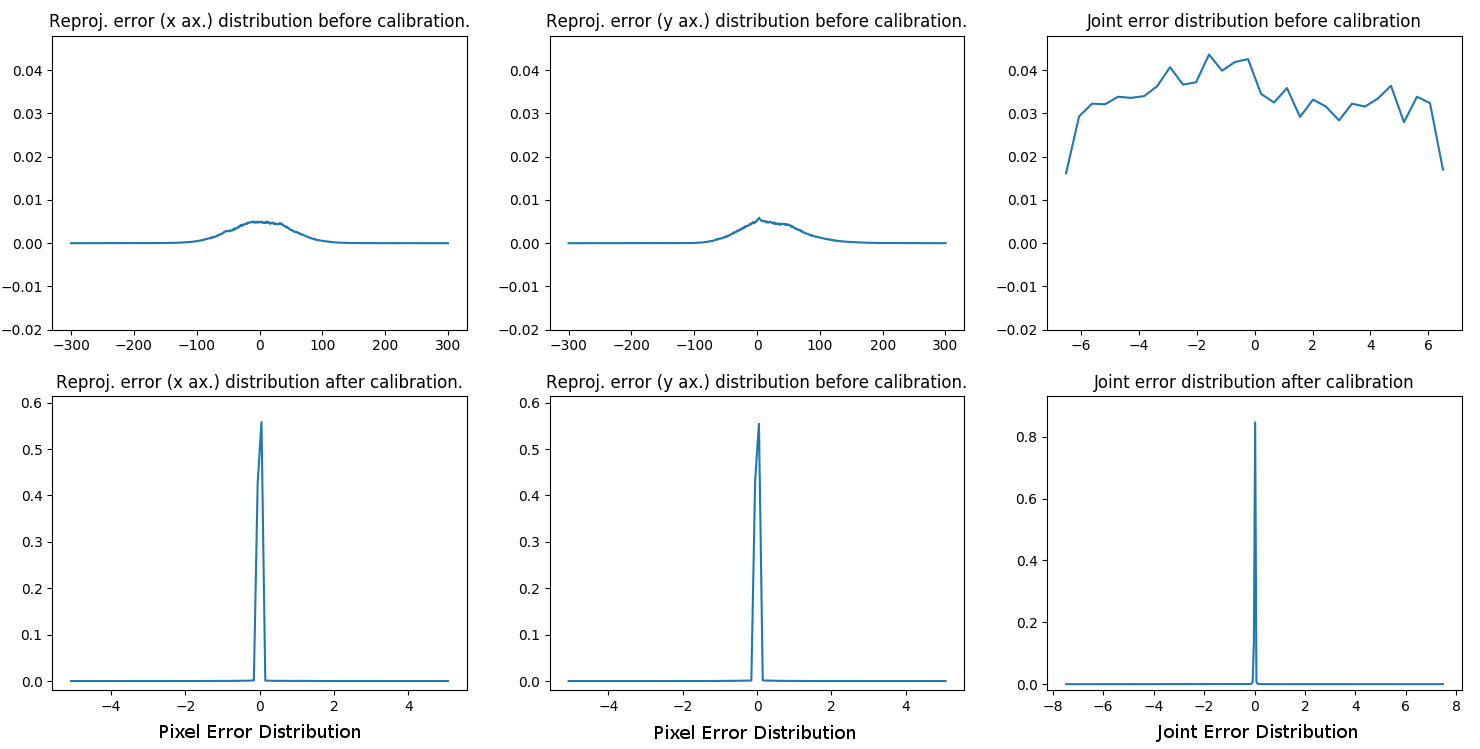
\includegraphics[width=0.9\paperwidth]{poselist-L-generic-L-LegaAndHeadUniRandErr0-6_5deg-pitchDiv2_stochastic_fix.png}
	}
	\captionof{figure}{Error distribution for $\pm6.5\degree$ error set. Top row is before calibration and Bottom row is after calibration. DO A BETTER PICTURE}
\end{center}

Based on results of this evaluation, it was evident that there is potential for further analysis so following sections cover important configurations which exhibited various results.

\section{Ground plane feature with simulated sensor noise}
\label{sec:ground_plane_test}

For the next phase of realism, sensor noise was introduced with other settings unchanged from initial evaluation described in \cref{tab:initial_test_config}. The reason for not immediately switching to sparsely positioned calibration patterns was due to need of identifying most suitable set of poses and effect of number of poses. By determining optimal amount of poses, identifying potential positions for calibration patterns for testing was simplified.

\begin{table}[]
	\resizebox{\textwidth}{!}{%
		\def\arraystretch{1.5}%  1 is the default, change whatever you need
		\begin{tabular}{@{}cccccccccc@{}}
			\toprule
			& \multicolumn{3}{c}{3 Poses}& \multicolumn{3}{c}{5 Poses}& \multicolumn{3}{c}{8 Poses}\\ \cmidrule(r{4pt}){2-4} \cmidrule(r{4pt}){5-7} \cmidrule(r{4pt}){8-10} 
			Noise Src. &  Succ.\% & LocMin.\% & Other\% & Succ.\% & LocMin.\% & Other\% & Succ.\% & LocMin.\% & Other\% \\ \cmidrule(r{4pt}){1-1} \cmidrule(r{4pt}){2-4} \cmidrule(r{4pt}){5-7} \cmidrule(r{4pt}){8-10} 
			noNoise &       87.02 & 12.94 & 0.04 &85.90 & 14.04 & 0.06 &83.94 & 15.90 & 0.16 \\ 
			pixel & 86.36 & 13.58 & 0.06 &84.64 & 15.30 & 0.06 &83.82 & 16.04 & 0.14 \\ 
			joint & 47.26 & 52.66 & 0.08 &53.74 & 46.22 & 0.04 &58.30 & 41.38 & 0.32 \\ 
			both &  46.56 & 53.36 & 0.08 &53.38 & 46.58 & 0.04 &57.32 & 42.52 & 0.16 \\ 
			\bottomrule
		\end{tabular}%
	}
	\caption[Results from testing with ground-plane calibration feature.]{Results from testing with ground-plane calibration feature. The results depicts several trends between calibration pose count, type of induced errors and success/ failure statistics}
\end{table}

The following conclusions can be taken based of results from this set of evaluations.
\begin{enumerate}
\item 
While minimum number of poses (3) provides highest success rate for no-noise conditions, it doesn't perform well with added noise.
\item 
Highest number of poses (8) performed 6.4\% better than minimal pose setup with joint noise alone and pixel + joint noise. However success rate was reduced by 1.1\% under no-noise.
\item
Pixel positioning noise affect success rate with more poses. Potentially due to effect of noise being higher than benefit of more captures.
\item
However, in case of joint noise, more poses clearly improved results. 
\item Perhaps the reason for this is due to higher ratio of image points to joint sensor measurements (hundreds vs 26).
\end{enumerate}


%\begin{figure}
%	\begin{subfigure}{\textwidth}
%		\centering
%		% This file was created by matplotlib2tikz v0.7.4.
\begin{tikzpicture}

\definecolor{color0}{rgb}{1,0.498039215686275,0.0549019607843137}
\definecolor{color1}{rgb}{0.501960784313725,0,0.501960784313725}

\begin{groupplot}[group style={group size=1 by 2}]
\nextgroupplot[
height=8cm,
tick align=outside,
tick pos=left,
width=15cm,
x grid style={white!69.01960784313725!black},
xmajorgrids,
xmin=-3.8499375, xmax=3.8495675,
xtick style={color=black},
y grid style={white!69.01960784313725!black},
ylabel={Joint number (excluding arms)},
ymin=0.5, ymax=14.5,
ytick style={color=black}
]
\addplot [black]
table {%
-3.4213225 0.75
-3.4213225 1.25
-3.2352575 1.25
-3.2352575 0.75
-3.4213225 0.75
};
\addplot [black]
table {%
-3.4213225 1
-3.48259 1
};
\addplot [black]
table {%
-3.2352575 1
-3.16846 1
};
\addplot [semithick, black, dashed]
table {%
-3.48259 0.875
-3.48259 1.125
};
\addplot [semithick, black, dashed]
table {%
-3.16846 0.875
-3.16846 1.125
};
\addplot [black, opacity=0.4, mark=*, mark size=1, mark options={solid,fill opacity=0,draw=color1}, only marks]
table {%
-3.49968 1
-3.49935 1
-3.49848 1
-3.49783 1
-3.49603 1
-3.49444 1
-3.49328 1
-3.49292 1
-3.49285 1
-3.49204 1
-3.49069 1
-3.49022 1
-3.49006 1
-3.48983 1
-3.48959 1
-3.4891 1
-3.48831 1
-3.48801 1
-3.4873 1
-3.48575 1
-3.48536 1
-3.48531 1
-3.48461 1
-3.48399 1
-3.48397 1
-3.16775 1
-3.16756 1
-3.1675 1
-3.16721 1
-3.16583 1
-3.16527 1
-3.16476 1
-3.16434 1
-3.16422 1
-3.16338 1
-3.16331 1
-3.1632 1
-3.16314 1
-3.16307 1
-3.16205 1
-3.16199 1
-3.16193 1
-3.16136 1
-3.16117 1
-3.16072 1
-3.16056 1
-3.16026 1
-3.15939 1
-3.15908 1
-3.15899 1
};
\addplot [black]
table {%
-0.92346575 1.75
-0.92346575 2.25
0 2.25
0 1.75
-0.92346575 1.75
};
\addplot [black]
table {%
-0.92346575 2
-1.55737 2
};
\addplot [black]
table {%
0 2
0 2
};
\addplot [semithick, black, dashed]
table {%
-1.55737 1.875
-1.55737 2.125
};
\addplot [semithick, black, dashed]
table {%
0 1.875
0 2.125
};
\addplot [black, opacity=0.4, mark=*, mark size=1, mark options={solid,fill opacity=0,draw=color1}, only marks]
table {%
-1.7046 2
-1.5757 2
-1.60402 2
-1.60485 2
-1.72168 2
-1.65899 2
-1.73001 2
-1.69169 2
-1.66628 2
-1.6946 2
-1.61068 2
-1.58485 2
-1.5859 2
-1.71313 2
-1.6063 2
-1.64504 2
-1.62275 2
-1.63983 2
-1.59131 2
-1.6694 2
-1.58548 2
-1.62254 2
-1.73104 2
-1.61151 2
-1.66357 2
};
\addplot [black]
table {%
-1.7633125 2.75
-1.7633125 3.25
1.84704 3.25
1.84704 2.75
-1.7633125 2.75
};
\addplot [black]
table {%
-1.7633125 3
-3.19867 3
};
\addplot [black]
table {%
1.84704 3
3.15525 3
};
\addplot [semithick, black, dashed]
table {%
-3.19867 2.875
-3.19867 3.125
};
\addplot [semithick, black, dashed]
table {%
3.15525 2.875
3.15525 3.125
};
\addplot [black, opacity=0.4, mark=*, mark size=1, mark options={solid,fill opacity=0,draw=color1}, only marks]
table {%
-3.32899 3
-3.41825 3
-3.32506 3
-3.25587 3
-3.24073 3
-3.34685 3
-3.42221 3
-3.24416 3
-3.20467 3
-3.49079 3
-3.24946 3
-3.26618 3
-3.22601 3
-3.30642 3
-3.38913 3
-3.20491 3
-3.45262 3
-3.47122 3
-3.41298 3
-3.23652 3
-3.35121 3
-3.22559 3
-3.37874 3
-3.23354 3
-3.21161 3
3.43936 3
3.38215 3
3.1742 3
3.1675 3
3.35602 3
3.27952 3
3.4919 3
3.39378 3
3.4153 3
3.29644 3
3.24298 3
3.26762 3
3.20688 3
3.42942 3
3.40016 3
3.33445 3
3.37649 3
3.1696 3
3.24808 3
3.46514 3
3.22941 3
3.40835 3
3.26059 3
3.241 3
3.43944 3
};
\addplot [black]
table {%
-1.7588475 3.75
-1.7588475 4.25
1.7216275 4.25
1.7216275 3.75
-1.7588475 3.75
};
\addplot [black]
table {%
-1.7588475 4
-3.08929 4
};
\addplot [black]
table {%
1.7216275 4
3.23933 4
};
\addplot [semithick, black, dashed]
table {%
-3.08929 3.875
-3.08929 4.125
};
\addplot [semithick, black, dashed]
table {%
3.23933 3.875
3.23933 4.125
};
\addplot [black, opacity=0.4, mark=*, mark size=1, mark options={solid,fill opacity=0,draw=color1}, only marks]
table {%
-3.26565 4
-3.34846 4
-3.44621 4
-3.34735 4
-3.1503 4
-3.46606 4
-3.16417 4
-3.23822 4
-3.42495 4
-3.38694 4
-3.38424 4
-3.14439 4
-3.46492 4
-3.09876 4
-3.09653 4
-3.32716 4
-3.41076 4
-3.41225 4
-3.45386 4
-3.2947 4
-3.49482 4
-3.46217 4
-3.10836 4
-3.20337 4
-3.25821 4
3.36571 4
3.25576 4
3.28733 4
3.40165 4
3.40405 4
3.38265 4
3.33355 4
3.33802 4
3.35833 4
3.40131 4
3.3381 4
3.27847 4
3.27257 4
3.48785 4
3.33816 4
3.45008 4
3.49364 4
3.277 4
3.29507 4
3.41342 4
3.46084 4
3.44713 4
3.23962 4
3.47116 4
3.24738 4
};
\addplot [black]
table {%
-1.7950925 4.75
-1.7950925 5.25
1.6174625 5.25
1.6174625 4.75
-1.7950925 4.75
};
\addplot [black]
table {%
-1.7950925 5
-3.17502 5
};
\addplot [black]
table {%
1.6174625 5
3.13203 5
};
\addplot [semithick, black, dashed]
table {%
-3.17502 4.875
-3.17502 5.125
};
\addplot [semithick, black, dashed]
table {%
3.13203 4.875
3.13203 5.125
};
\addplot [black, opacity=0.4, mark=*, mark size=1, mark options={solid,fill opacity=0,draw=color1}, only marks]
table {%
-3.44312 5
-3.2193 5
-3.19733 5
-3.24723 5
-3.43659 5
-3.44414 5
-3.48237 5
-3.25855 5
-3.40744 5
-3.39005 5
-3.32659 5
-3.29662 5
-3.27299 5
-3.39217 5
-3.44345 5
-3.28065 5
-3.39543 5
-3.2934 5
-3.34975 5
-3.46563 5
-3.48818 5
-3.25686 5
-3.42405 5
-3.17775 5
-3.34039 5
3.37013 5
3.49948 5
3.39473 5
3.35041 5
3.44236 5
3.2665 5
3.37304 5
3.30464 5
3.34045 5
3.36345 5
3.45753 5
3.43064 5
3.23278 5
3.25016 5
3.18108 5
3.47304 5
3.29182 5
3.35137 5
3.38193 5
3.19081 5
3.14754 5
3.13729 5
3.42188 5
3.3029 5
3.15803 5
};
\addplot [black]
table {%
-1.542945 5.75
-1.542945 6.25
1.7872125 6.25
1.7872125 5.75
-1.542945 5.75
};
\addplot [black]
table {%
-1.542945 6
-2.9961 6
};
\addplot [black]
table {%
1.7872125 6
3.15726 6
};
\addplot [semithick, black, dashed]
table {%
-2.9961 5.875
-2.9961 6.125
};
\addplot [semithick, black, dashed]
table {%
3.15726 5.875
3.15726 6.125
};
\addplot [black, opacity=0.4, mark=*, mark size=1, mark options={solid,fill opacity=0,draw=color1}, only marks]
table {%
-3.06497 6
-3.49996 6
-3.13521 6
-3.29569 6
-3.48295 6
-3.26576 6
-3.20246 6
-3.236 6
-3.19729 6
-3.32387 6
-3.42134 6
-3.18319 6
-3.00696 6
-3.04594 6
-3.4188 6
-3.06618 6
-3.00756 6
-3.00756 6
-3.13287 6
-3.29869 6
-3.36904 6
-3.27774 6
-3.43748 6
-3.2125 6
-3.25541 6
3.49884 6
3.23924 6
3.31649 6
3.4829 6
3.3505 6
3.3225 6
3.33981 6
3.27278 6
3.36433 6
3.34696 6
3.42965 6
3.34697 6
3.1586 6
3.3932 6
3.22091 6
3.39998 6
3.30654 6
3.43417 6
3.46798 6
3.35634 6
3.49724 6
3.28454 6
3.37325 6
3.23961 6
3.42193 6
};
\addplot [black]
table {%
-1.6247175 6.75
-1.6247175 7.25
1.8622775 7.25
1.8622775 6.75
-1.6247175 6.75
};
\addplot [black]
table {%
-1.6247175 7
-3.07764 7
};
\addplot [black]
table {%
1.8622775 7
3.09452 7
};
\addplot [semithick, black, dashed]
table {%
-3.07764 6.875
-3.07764 7.125
};
\addplot [semithick, black, dashed]
table {%
3.09452 6.875
3.09452 7.125
};
\addplot [black, opacity=0.4, mark=*, mark size=1, mark options={solid,fill opacity=0,draw=color1}, only marks]
table {%
-3.40558 7
-3.21411 7
-3.1999 7
-3.22484 7
-3.10627 7
-3.45749 7
-3.48965 7
-3.25454 7
-3.2613 7
-3.20799 7
-3.49398 7
-3.37504 7
-3.11637 7
-3.38067 7
-3.08896 7
-3.20581 7
-3.4577 7
-3.34362 7
-3.37451 7
-3.45153 7
-3.47485 7
-3.3646 7
-3.23723 7
-3.4861 7
-3.45201 7
3.11431 7
3.49249 7
3.31091 7
3.1089 7
3.46961 7
3.16773 7
3.37803 7
3.39252 7
3.26766 7
3.46972 7
3.14162 7
3.42924 7
3.16542 7
3.11557 7
3.34307 7
3.38169 7
3.31601 7
3.4384 7
3.13614 7
3.35894 7
3.17286 7
3.17224 7
3.47062 7
3.1087 7
3.43726 7
};
\addplot [black]
table {%
-1.8140875 7.75
-1.8140875 8.25
1.67165 8.25
1.67165 7.75
-1.8140875 7.75
};
\addplot [black]
table {%
-1.8140875 8
-3.07792 8
};
\addplot [black]
table {%
1.67165 8
3.14176 8
};
\addplot [semithick, black, dashed]
table {%
-3.07792 7.875
-3.07792 8.125
};
\addplot [semithick, black, dashed]
table {%
3.14176 7.875
3.14176 8.125
};
\addplot [black, opacity=0.4, mark=*, mark size=1, mark options={solid,fill opacity=0,draw=color1}, only marks]
table {%
-3.08581 8
-3.29419 8
-3.30353 8
-3.28388 8
-3.22768 8
-3.09143 8
-3.45143 8
-3.3576 8
-3.38654 8
-3.34614 8
-3.28709 8
-3.25298 8
-3.44298 8
-3.4292 8
-3.32556 8
-3.42591 8
-3.38899 8
-3.46319 8
-3.32526 8
-3.13838 8
-3.37626 8
-3.38504 8
-3.38101 8
-3.35235 8
-3.40464 8
3.30734 8
3.41317 8
3.43548 8
3.24258 8
3.2841 8
3.49959 8
3.25678 8
3.32817 8
3.29108 8
3.17286 8
3.20136 8
3.32051 8
3.25712 8
3.33117 8
3.30985 8
3.36501 8
3.29061 8
3.47264 8
3.46109 8
3.32304 8
3.24538 8
3.21715 8
3.47478 8
3.36265 8
3.23859 8
};
\addplot [black]
table {%
0 8.75
0 9.25
0 9.25
0 8.75
0 8.75
};
\addplot [black]
table {%
0 9
0 9
};
\addplot [black]
table {%
0 9
0 9
};
\addplot [semithick, black, dashed]
table {%
0 8.875
0 9.125
};
\addplot [semithick, black, dashed]
table {%
0 8.875
0 9.125
};
\addplot [black]
table {%
0 9.75
0 10.25
0 10.25
0 9.75
0 9.75
};
\addplot [black]
table {%
0 10
0 10
};
\addplot [black]
table {%
0 10
0 10
};
\addplot [semithick, black, dashed]
table {%
0 9.875
0 10.125
};
\addplot [semithick, black, dashed]
table {%
0 9.875
0 10.125
};
\addplot [black]
table {%
0 10.75
0 11.25
0 11.25
0 10.75
0 10.75
};
\addplot [black]
table {%
0 11
0 11
};
\addplot [black]
table {%
0 11
0 11
};
\addplot [semithick, black, dashed]
table {%
0 10.875
0 11.125
};
\addplot [semithick, black, dashed]
table {%
0 10.875
0 11.125
};
\addplot [black]
table {%
0 11.75
0 12.25
0 12.25
0 11.75
0 11.75
};
\addplot [black]
table {%
0 12
0 12
};
\addplot [black]
table {%
0 12
0 12
};
\addplot [semithick, black, dashed]
table {%
0 11.875
0 12.125
};
\addplot [semithick, black, dashed]
table {%
0 11.875
0 12.125
};
\addplot [black]
table {%
0 12.75
0 13.25
0 13.25
0 12.75
0 12.75
};
\addplot [black]
table {%
0 13
0 13
};
\addplot [black]
table {%
0 13
0 13
};
\addplot [semithick, black, dashed]
table {%
0 12.875
0 13.125
};
\addplot [semithick, black, dashed]
table {%
0 12.875
0 13.125
};
\addplot [black]
table {%
0 13.75
0 14.25
0 14.25
0 13.75
0 13.75
};
\addplot [black]
table {%
0 14
0 14
};
\addplot [black]
table {%
0 14
0 14
};
\addplot [semithick, black, dashed]
table {%
0 13.875
0 14.125
};
\addplot [semithick, black, dashed]
table {%
0 13.875
0 14.125
};
\addplot [color0]
table {%
-3.335975 0.75
-3.335975 1.25
};
\addplot [color0]
table {%
0 1.75
0 2.25
};
\addplot [color0]
table {%
0.035474295 2.75
0.035474295 3.25
};
\addplot [color0]
table {%
-0.1035925 3.75
-0.1035925 4.25
};
\addplot [color0]
table {%
0.0744103 4.75
0.0744103 5.25
};
\addplot [color0]
table {%
0.460234 5.75
0.460234 6.25
};
\addplot [color0]
table {%
-0.134443 6.75
-0.134443 7.25
};
\addplot [color0]
table {%
-0.1399855 7.75
-0.1399855 8.25
};
\addplot [color0]
table {%
0 8.75
0 9.25
};
\addplot [color0]
table {%
0 9.75
0 10.25
};
\addplot [color0]
table {%
0 10.75
0 11.25
};
\addplot [color0]
table {%
0 11.75
0 12.25
};
\addplot [color0]
table {%
0 12.75
0 13.25
};
\addplot [color0]
table {%
0 13.75
0 14.25
};

\nextgroupplot[
height=8cm,
tick align=outside,
tick pos=left,
width=15cm,
x grid style={white!69.01960784313725!black},
xmin=-3.8499375, xmax=3.8495675,
xtick style={color=black},
y grid style={white!69.01960784313725!black},
ymin=0, ymax=1,
ytick style={color=black},
ytick={0,0.2,0.4,0.6,0.8,1},
yticklabels={0.0,0.2,0.4,0.6,0.8,1.0}
]
\end{groupplot}

\end{tikzpicture}
%		\caption{before}
%		\label{fig:sfig1}
%	\end{subfigure}%
%
%	\begin{subfigure}{\textwidth}
%		\centering
%		% This file was created by matplotlib2tikz v0.7.4.
\begin{tikzpicture}

\definecolor{color0}{rgb}{1,0.498039215686275,0.0549019607843137}
\definecolor{color1}{rgb}{0.501960784313725,0,0.501960784313725}

\begin{axis}[
height=8cm,
tick align=outside,
tick pos=left,
title={Joint error distribution after calibration},
width=15cm,
x grid style={white!69.01960784313725!black},
xlabel={Error distribution (\(\displaystyle \degree\))},
xmajorgrids,
xmin=-8, xmax=8,
xtick style={color=black},
y grid style={white!69.01960784313725!black},
ylabel={Joint},
ymin=0.5, ymax=14.5,
ytick style={color=black},
ytick={1,2,3,4,5,6,7,8,9,10,11,12,13,14},
yticklabels={HEAD\_Y,HEAD\_P,L\_HIP\_YP,L\_HIP\_R,L\_HIP\_P,L\_KNEE\_P,L\_ANKL\_P,L\_ANKL\_R,R\_HIP\_YP,R\_HIP\_R,R\_HIP\_P,R\_KNEE\_P,R\_ANKL\_P,R\_ANKL\_R}
]
\addplot [black]
table {%
-0.05817515 0.75
-0.05817515 1.25
0.054659725 1.25
0.054659725 0.75
-0.05817515 0.75
};
\addplot [black]
table {%
-0.05817515 1
-0.226426 1
};
\addplot [black]
table {%
0.054659725 1
0.222448 1
};
\addplot [semithick, black, dashed]
table {%
-0.226426 0.875
-0.226426 1.125
};
\addplot [semithick, black, dashed]
table {%
0.222448 0.875
0.222448 1.125
};
\addplot [black, opacity=0.4, mark=*, mark size=1, mark options={solid,fill opacity=0,draw=color1}, only marks]
table {%
-0.275618 1
-0.332816 1
-0.303778 1
-0.302124 1
-0.375157 1
-0.398667 1
-0.475435 1
-0.26388 1
-0.342619 1
-0.388914 1
-0.619701 1
-0.228038 1
-2.93076 1
-0.541789 1
-0.397593 1
-0.337391 1
-0.378558 1
-13.8551 1
-0.299337 1
-35.4625 1
-0.234203 1
-0.290451 1
-0.662627 1
-0.483191 1
-1.09681 1
-0.339798 1
-0.74161 1
-2.03918 1
-4.47223 1
-0.512267 1
-0.339074 1
-0.456811 1
-0.825903 1
-0.441323 1
-0.929351 1
-0.494013 1
-0.245919 1
-0.399567 1
-0.409692 1
-0.35376 1
-0.238217 1
-0.679596 1
-0.340413 1
-0.435904 1
-0.369132 1
-0.254205 1
-0.345023 1
-10.1431 1
-0.474368 1
-0.526026 1
-0.50737 1
-0.282664 1
-0.229047 1
-0.3721 1
-0.508277 1
-0.464998 1
-0.254954 1
-0.309392 1
-0.307976 1
-0.344331 1
-0.332165 1
-0.368086 1
-0.311559 1
-4.26856 1
-0.312862 1
-0.859788 1
-0.661087 1
-0.862978 1
-0.321259 1
-0.359475 1
-0.35461 1
-0.312914 1
-0.3366 1
-0.511552 1
-0.552935 1
-0.234637 1
-0.283671 1
-0.588329 1
-0.370407 1
-0.612064 1
-0.533456 1
-0.403989 1
-0.341841 1
-0.425438 1
-1.28074 1
-0.325663 1
-0.264153 1
-0.361206 1
-0.424798 1
-0.256919 1
-0.655939 1
-0.33071 1
-0.241968 1
-0.957767 1
-2.90988 1
-0.320621 1
-0.267979 1
-0.567091 1
-0.749181 1
-0.295669 1
-0.247275 1
-0.233438 1
-0.259626 1
-0.377627 1
-0.331983 1
-0.53299 1
-0.255925 1
-0.689021 1
-0.353121 1
-0.396033 1
-0.258798 1
-0.270727 1
-0.348206 1
-0.668299 1
-0.396159 1
-0.381117 1
-0.383078 1
-0.281496 1
-0.236766 1
-0.308222 1
-4.71346 1
-0.331377 1
-0.491488 1
-0.321147 1
-0.649976 1
-13.3144 1
-0.520116 1
-0.398514 1
-0.279328 1
-0.238601 1
-0.392549 1
-0.386476 1
-0.240232 1
-0.481375 1
-0.339524 1
-0.555986 1
-0.522104 1
-0.473049 1
-0.58758 1
-0.280722 1
-0.304141 1
-0.592107 1
-0.626392 1
-0.243323 1
-0.400025 1
-0.352094 1
-0.311135 1
-0.246103 1
-0.277108 1
-16.1216 1
-18.4694 1
-0.468939 1
-0.242965 1
-0.381086 1
-0.237868 1
-0.370627 1
-0.267188 1
-0.269189 1
-0.809027 1
-3.32856 1
-0.360949 1
-0.324022 1
-0.406568 1
-0.389221 1
-0.30084 1
-0.494151 1
-0.251988 1
-0.451031 1
-0.251323 1
-0.310832 1
-0.650758 1
-0.953637 1
-0.275467 1
-0.25 1
-0.611297 1
-0.529613 1
-0.248692 1
-0.574875 1
-0.428959 1
-0.447289 1
-0.397613 1
-0.251363 1
-0.245157 1
-0.336799 1
-0.333121 1
-0.317086 1
-0.273722 1
-0.397194 1
-0.251845 1
-0.356797 1
-0.38127 1
-0.603259 1
-0.977163 1
-1.77779 1
-0.474539 1
-0.446167 1
-0.463994 1
-0.245375 1
-0.407879 1
-0.475418 1
-0.29859 1
-0.435629 1
-0.323721 1
-6.43493 1
-4.11835 1
-0.239602 1
-0.4089 1
-0.600062 1
-0.819376 1
-0.84082 1
-0.345966 1
-1.10116 1
-0.337872 1
-0.309438 1
-0.848981 1
-0.391595 1
-0.742388 1
-0.241555 1
-0.518138 1
-0.283911 1
-0.422489 1
-0.616347 1
-0.542712 1
-0.445683 1
-0.328549 1
-0.259917 1
-0.369267 1
-0.290914 1
-0.420409 1
-0.47097 1
-4.28017 1
-0.364521 1
-0.545629 1
-0.595059 1
-0.453107 1
-0.434316 1
-0.266022 1
-0.515536 1
-0.302529 1
-0.739241 1
-0.554038 1
-0.768675 1
-0.368674 1
-0.263202 1
-0.241054 1
-0.33658 1
-0.236329 1
-0.430238 1
-0.294493 1
-0.422973 1
-0.501121 1
-0.424104 1
-0.279063 1
-0.42231 1
-0.253134 1
-0.393557 1
-0.286443 1
-0.33713 1
-0.277374 1
-0.565912 1
-0.34367 1
-0.391043 1
-0.678623 1
-7.36692 1
-0.492399 1
-0.393924 1
-0.324368 1
-0.245081 1
-0.684579 1
-0.250309 1
-0.333198 1
-0.263957 1
-0.242155 1
-0.318302 1
-0.538622 1
-0.522052 1
-0.636484 1
-0.318021 1
-0.654122 1
-0.227471 1
-0.269824 1
-0.636165 1
-0.989134 1
-0.267221 1
-1.27328 1
-0.386933 1
-0.719554 1
-63.6113 1
-0.460959 1
-0.424255 1
-0.310509 1
-0.468811 1
-0.439083 1
-0.499305 1
-0.686097 1
-0.323071 1
-0.231443 1
-1.38098 1
-0.291047 1
-0.239839 1
-0.287305 1
-0.552183 1
-0.745862 1
-0.630531 1
-0.266266 1
-0.298333 1
-0.406333 1
-0.460303 1
-0.324027 1
-0.781836 1
-0.258374 1
-0.292103 1
-0.254461 1
-0.233083 1
-0.244835 1
-0.667016 1
-0.315168 1
-0.656959 1
-0.307768 1
-0.679997 1
-0.379226 1
-0.304181 1
-1.18182 1
-0.417491 1
-0.558603 1
-0.355799 1
-8.40159 1
-0.263968 1
-0.261829 1
-0.266975 1
-0.574452 1
-0.272449 1
-0.628181 1
-0.265666 1
-0.27279 1
-0.664571 1
-0.460666 1
-0.680848 1
-0.258621 1
-0.254401 1
-0.682328 1
-0.337053 1
-0.85376 1
-0.290826 1
-0.268315 1
-0.405601 1
-0.419641 1
-0.281311 1
-0.471688 1
-0.625903 1
-0.346855 1
-0.402022 1
-0.289478 1
-0.393085 1
-0.274983 1
-0.232998 1
-0.315163 1
-0.369136 1
-1.04639 1
-0.888652 1
-0.505998 1
-0.234725 1
-0.663141 1
-0.266502 1
-0.47633 1
-0.253119 1
-0.257605 1
-0.845362 1
-0.361718 1
-0.299009 1
-0.284957 1
-0.29735 1
-0.254952 1
-0.255858 1
-0.488288 1
-0.300244 1
-0.477404 1
-0.558125 1
-0.631967 1
-0.279505 1
-0.44007 1
-0.250656 1
-0.266274 1
-0.542061 1
-0.331403 1
-0.34947 1
-0.257616 1
-0.359683 1
-0.417139 1
-0.28812 1
-0.644054 1
-0.267073 1
-0.258241 1
-0.539169 1
-0.300607 1
-0.268977 1
-0.624008 1
-0.472675 1
-0.47992 1
-0.252903 1
-0.655283 1
-0.301718 1
-0.525808 1
-0.93569 1
-0.359471 1
-0.421592 1
-0.444989 1
-1.60402 1
-1.88891 1
-0.242577 1
-0.311477 1
-0.373317 1
-0.31375 1
-0.251884 1
-0.840672 1
-0.288166 1
-0.28748 1
-0.265526 1
-0.527967 1
-0.251736 1
-0.372361 1
-0.736552 1
-1.14034 1
-0.514094 1
-0.449704 1
-0.430633 1
-0.344846 1
-0.284942 1
-0.367696 1
-0.673323 1
-0.532617 1
-0.23178 1
-0.237942 1
-0.253729 1
-0.254028 1
-0.244117 1
-0.424956 1
-0.606384 1
-0.392721 1
-0.26202 1
-0.379787 1
-0.483535 1
-0.245161 1
-0.440933 1
-0.383981 1
-0.399507 1
-0.242788 1
-0.546081 1
-0.320537 1
-0.822483 1
-0.653057 1
-0.528888 1
-1.03706 1
-0.794722 1
-1.95242 1
-0.342153 1
-0.294917 1
-0.332393 1
-0.267434 1
-0.27288 1
-0.543836 1
-0.262716 1
-0.284195 1
-0.231241 1
-0.263752 1
-0.302904 1
-1.03098 1
-0.398607 1
-1.6223 1
-0.250809 1
-0.349283 1
-9.2303 1
-0.239065 1
-0.447581 1
-0.354861 1
-0.320494 1
0.590545 1
1.39027 1
0.556704 1
0.402833 1
0.380524 1
1.05307 1
0.262109 1
0.315191 1
0.284906 1
0.268451 1
0.257515 1
0.502935 1
0.487052 1
0.339261 1
2.71383 1
0.52354 1
0.956143 1
0.313618 1
0.409139 1
0.903269 1
0.259061 1
0.300119 1
0.519957 1
6.97632 1
1.15743 1
0.456036 1
0.707437 1
0.625339 1
5.5053 1
0.582934 1
0.251522 1
0.555393 1
0.413667 1
0.391482 1
0.264107 1
0.837377 1
0.601207 1
0.725221 1
9.25809 1
0.263775 1
0.297189 1
2.071 1
0.259694 1
0.355384 1
1.29821 1
9.06463 1
0.470604 1
0.467236 1
0.263703 1
0.238622 1
0.654916 1
0.379088 1
0.227448 1
0.449504 1
0.292773 1
0.251021 1
0.355786 1
12.8648 1
0.289496 1
0.356455 1
0.576173 1
0.25709 1
0.266639 1
0.277088 1
0.254518 1
0.530687 1
0.428275 1
0.92921 1
1.88999 1
0.985667 1
0.248892 1
0.312565 1
0.644858 1
0.569357 1
1.43647 1
16.4569 1
0.333632 1
0.27409 1
0.535304 1
0.628304 1
0.564873 1
0.2383 1
0.38407 1
0.261343 1
0.289276 1
0.319117 1
0.252098 1
0.681156 1
0.811722 1
0.235216 1
0.549566 1
1.03374 1
0.57448 1
0.417512 1
0.327593 1
0.305722 1
0.652105 1
0.651673 1
0.804585 1
0.558589 1
0.330951 1
0.265724 1
0.466274 1
0.547577 1
0.768604 1
0.486099 1
0.321099 1
0.529922 1
0.660999 1
0.348405 1
0.432986 1
0.469147 1
0.26671 1
0.362327 1
0.411956 1
0.472574 1
0.283321 1
1.03924 1
0.321174 1
0.43277 1
2.09886 1
0.402354 1
0.347162 1
0.499499 1
0.282057 1
0.364809 1
0.286675 1
0.881863 1
0.389159 1
0.602891 1
0.270135 1
0.355238 1
0.275649 1
0.439434 1
0.226504 1
0.257167 1
0.245664 1
0.750817 1
0.788751 1
0.512876 1
0.944357 1
0.447256 1
0.407095 1
0.338802 1
0.401821 1
0.266744 1
0.284156 1
0.369028 1
7.10692 1
0.263396 1
0.594555 1
0.31342 1
0.445071 1
0.371821 1
0.386722 1
0.485817 1
0.229327 1
0.556017 1
0.747475 1
0.286944 1
0.493362 1
0.435745 1
0.458879 1
0.569952 1
0.347155 1
0.31324 1
0.635918 1
0.28062 1
0.387787 1
0.435881 1
0.397888 1
0.312158 1
0.513045 1
0.620705 1
0.25295 1
0.462759 1
0.544678 1
0.260676 1
0.452646 1
0.655027 1
0.770942 1
0.280746 1
0.238713 1
0.735938 1
0.230108 1
0.43294 1
0.337554 1
0.901316 1
0.537272 1
0.300039 1
0.287466 1
0.308312 1
0.364576 1
0.533655 1
0.883467 1
0.375832 1
0.241005 1
0.248124 1
0.292012 1
0.306548 1
0.706503 1
0.567884 1
0.224233 1
0.390443 1
0.267069 1
0.33349 1
0.257509 1
0.22887 1
0.544839 1
0.243657 1
0.238263 1
0.448198 1
0.389493 1
0.389645 1
0.443444 1
0.728981 1
0.233953 1
0.55602 1
0.698412 1
0.373273 1
0.397881 1
0.275863 1
0.535778 1
0.552355 1
0.232516 1
0.391747 1
0.492041 1
0.420331 1
0.494233 1
0.396552 1
0.339605 1
0.52137 1
0.227672 1
0.525259 1
0.261815 1
0.345761 1
0.589663 1
0.385946 1
0.233238 1
0.490125 1
0.232246 1
0.291333 1
0.509245 1
0.225071 1
0.555963 1
0.292232 1
0.554425 1
0.396535 1
0.439902 1
0.698219 1
0.307938 1
0.308666 1
0.330705 1
0.406303 1
0.238084 1
0.385276 1
0.490234 1
15.6935 1
0.337677 1
0.417407 1
0.357151 1
0.4092 1
0.366995 1
0.558559 1
0.491986 1
0.245885 1
1.23869 1
0.511101 1
0.51696 1
0.271817 1
0.449417 1
0.267944 1
0.288127 1
0.468995 1
0.45422 1
9.93968 1
0.245464 1
0.289475 1
0.280199 1
0.383651 1
0.484475 1
0.519532 1
0.296658 1
0.250685 1
0.579999 1
0.650806 1
0.751578 1
0.48928 1
0.377194 1
0.405844 1
0.391268 1
0.244049 1
0.728538 1
0.244003 1
1.85428 1
0.230721 1
0.374617 1
0.915347 1
0.670235 1
0.266174 1
5.5883 1
0.436687 1
0.374895 1
0.294987 1
0.572907 1
0.367448 1
0.508202 1
0.381146 1
0.337182 1
0.35819 1
0.295668 1
0.27101 1
0.423207 1
0.273576 1
0.781786 1
0.251176 1
0.280695 1
0.304885 1
0.51648 1
0.269618 1
0.543836 1
0.598855 1
2.21044 1
0.22507 1
0.747088 1
0.241678 1
0.248702 1
0.280989 1
0.650349 1
0.416949 1
0.48844 1
0.410672 1
0.640845 1
0.227134 1
0.341489 1
0.474103 1
0.387194 1
0.484892 1
0.843685 1
0.284047 1
0.361056 1
0.2805 1
0.274892 1
0.438938 1
0.338882 1
0.239481 1
0.318869 1
0.71661 1
0.42994 1
0.616538 1
0.705771 1
0.66874 1
0.647074 1
0.313178 1
0.517885 1
0.246439 1
0.225226 1
0.358006 1
0.478105 1
0.586884 1
0.269127 1
0.485741 1
0.258219 1
0.233618 1
0.792162 1
0.681557 1
0.344112 1
0.253912 1
0.420138 1
0.470659 1
0.246226 1
0.226721 1
0.748217 1
0.386286 1
0.344653 1
0.685621 1
0.440935 1
0.486643 1
0.416329 1
0.291084 1
0.755772 1
0.247288 1
0.63382 1
0.346276 1
0.29351 1
0.639735 1
0.418218 1
0.230598 1
0.629966 1
0.387384 1
0.594654 1
0.686381 1
0.401923 1
0.242114 1
0.24826 1
0.426339 1
1.10271 1
0.239874 1
0.255002 1
0.327819 1
0.545018 1
0.356253 1
0.393994 1
0.248062 1
0.504205 1
0.41906 1
0.31068 1
0.261861 1
0.367267 1
0.36108 1
0.304775 1
0.27909 1
0.346891 1
0.338241 1
1.74622 1
0.68849 1
0.89052 1
0.232529 1
0.810502 1
0.36226 1
0.361127 1
0.565955 1
0.336456 1
0.318031 1
0.535094 1
0.303442 1
0.348626 1
0.494126 1
0.225012 1
1.87177 1
0.313592 1
0.233442 1
0.424959 1
0.313023 1
0.259371 1
0.433674 1
0.538719 1
0.484844 1
0.438078 1
0.243426 1
0.352098 1
0.483633 1
0.271111 1
0.27075 1
0.438787 1
0.306848 1
0.412703 1
0.304921 1
0.320858 1
0.24959 1
0.382075 1
0.392964 1
0.439625 1
0.279709 1
0.298419 1
0.665479 1
0.238802 1
0.238194 1
0.277933 1
0.388676 1
0.25137 1
0.245609 1
0.333141 1
0.251361 1
0.57498 1
0.272349 1
0.270671 1
0.419234 1
0.285536 1
0.348258 1
0.300983 1
0.268838 1
0.521652 1
0.397634 1
};
\addplot [black]
table {%
-0.019455025 1.75
-0.019455025 2.25
0.01827515 2.25
0.01827515 1.75
-0.019455025 1.75
};
\addplot [black]
table {%
-0.019455025 2
-0.0759227 2
};
\addplot [black]
table {%
0.01827515 2
0.0745185 2
};
\addplot [semithick, black, dashed]
table {%
-0.0759227 1.875
-0.0759227 2.125
};
\addplot [semithick, black, dashed]
table {%
0.0745185 1.875
0.0745185 2.125
};
\addplot [black, opacity=0.4, mark=*, mark size=1, mark options={solid,fill opacity=0,draw=color1}, only marks]
table {%
-0.115297 2
-0.228961 2
-0.15559 2
-0.0767526 2
-0.202684 2
-0.0993444 2
-0.0891974 2
-0.0912368 2
-0.190833 2
-0.272007 2
-0.143447 2
-0.339767 2
-0.215775 2
-0.149978 2
-0.213956 2
-0.167501 2
-0.170238 2
-0.139741 2
-0.566105 2
-0.133539 2
-0.158895 2
-0.120486 2
-0.108575 2
-0.201829 2
-0.11698 2
-0.445071 2
-0.481245 2
-0.128626 2
-0.204998 2
-0.272972 2
-0.143652 2
-0.103949 2
-0.0913572 2
-0.114848 2
-0.0820222 2
-0.082459 2
-0.0916815 2
-0.38615 2
-0.425051 2
-0.645716 2
-0.164019 2
-0.386352 2
-1.28215 2
-6.27926 2
-0.586977 2
-0.15504 2
-0.142011 2
-0.167748 2
-0.181736 2
-0.289427 2
-0.450901 2
-0.124268 2
-0.135419 2
-0.590766 2
-0.120209 2
-0.262696 2
-0.124577 2
-0.196385 2
-0.124225 2
-0.0865948 2
-0.338166 2
-0.380836 2
-0.603922 2
-0.106556 2
-0.216546 2
-0.204183 2
-0.156216 2
-7.77517 2
-0.301122 2
-0.396127 2
-0.100341 2
-0.226985 2
-0.30398 2
-0.0799416 2
-0.0918801 2
-0.257805 2
-0.483326 2
-0.170643 2
-0.0977943 2
-0.111674 2
-0.113676 2
-0.246395 2
-0.361774 2
-0.252689 2
-0.0819694 2
-0.150291 2
-0.157114 2
-0.277212 2
-0.174514 2
-0.123111 2
-0.111688 2
-0.510273 2
-0.287223 2
-0.599748 2
-0.459873 2
-0.101774 2
-0.0910878 2
-0.108509 2
-0.53448 2
-0.216765 2
-0.0801021 2
-0.218351 2
-0.105957 2
-0.177286 2
-0.195293 2
-0.225149 2
-0.312019 2
-0.0903568 2
-0.0934897 2
-0.173323 2
-0.162112 2
-0.197896 2
-0.0953502 2
-0.226898 2
-0.156939 2
-0.141683 2
-9.39745 2
-0.32558 2
-0.183319 2
-0.164905 2
-0.0815732 2
-0.314594 2
-0.49317 2
-0.1002 2
-0.0992089 2
-0.0823837 2
-0.261266 2
-0.26196 2
-0.101528 2
-0.08556 2
-0.420572 2
-0.184625 2
-0.123144 2
-0.1565 2
-0.122521 2
-0.582274 2
-6.98503 2
-0.12093 2
-0.119879 2
-0.118045 2
-0.092884 2
-0.359096 2
-0.308262 2
-0.166747 2
-0.149755 2
-0.105247 2
-0.0887531 2
-0.122409 2
-0.155109 2
-0.207608 2
-0.276261 2
-0.292133 2
-0.316048 2
-0.270767 2
-0.145122 2
-0.107221 2
-0.153561 2
-0.116447 2
-0.204126 2
-0.176606 2
-0.234042 2
-0.380082 2
-0.1723 2
-0.167685 2
-0.107356 2
-0.207157 2
-0.196059 2
-0.161015 2
-0.152824 2
-0.147267 2
-0.129729 2
-0.306507 2
-0.0850542 2
-0.112434 2
-0.306782 2
-0.375698 2
-0.141074 2
-0.151939 2
-0.131683 2
-0.230005 2
-0.0925274 2
-0.228663 2
-0.25759 2
-0.151019 2
-0.283525 2
-0.375977 2
-0.268591 2
-0.0967593 2
-0.198585 2
-0.175911 2
-0.146061 2
-0.365504 2
-0.190758 2
-0.0899678 2
-0.182136 2
-0.300761 2
-0.227793 2
-4.75649 2
-0.308333 2
-0.0792016 2
-0.0996271 2
-0.0893684 2
-0.124798 2
-0.129801 2
-0.148486 2
-0.135959 2
-0.136467 2
-0.0824427 2
-0.0767592 2
-0.16407 2
-0.274726 2
-0.163381 2
-0.165827 2
-0.127018 2
-0.0938098 2
-0.385591 2
-0.21015 2
-0.192588 2
-0.118592 2
-0.109267 2
-0.44912 2
-5.695 2
-0.122946 2
-0.181149 2
-0.138992 2
-0.205165 2
-0.121 2
-0.23202 2
-0.185355 2
-0.345006 2
-0.15678 2
-0.151043 2
-0.23612 2
-0.172758 2
-0.0891425 2
-0.138274 2
-0.0904951 2
-0.394907 2
-0.116269 2
-0.180314 2
-0.548453 2
-0.192918 2
-0.11967 2
-0.420387 2
-0.240221 2
-0.189672 2
-0.0982182 2
-0.118922 2
-0.389235 2
-0.125721 2
-0.214021 2
-0.233324 2
-0.241896 2
-0.17911 2
-0.270791 2
-0.123529 2
-0.209291 2
-0.220736 2
-0.210552 2
-0.16013 2
-0.108449 2
-0.131896 2
-0.125592 2
-0.118999 2
-0.44351 2
-0.145438 2
-0.159213 2
-0.128347 2
-0.172995 2
-0.121979 2
-0.101173 2
-0.275913 2
-0.0835165 2
-0.120482 2
-0.997849 2
-1.28763 2
-0.279074 2
-0.17851 2
-0.252016 2
-0.300914 2
-0.297949 2
-0.0972666 2
-0.330667 2
-0.189355 2
-0.353256 2
-0.171594 2
-0.108348 2
-8.70671 2
-0.0940278 2
-0.218166 2
-0.415931 2
-0.0882713 2
-0.116788 2
-0.50369 2
-0.187543 2
-0.597698 2
-0.493696 2
-0.177051 2
-0.0978681 2
-0.405129 2
-0.179508 2
-0.287516 2
-0.547417 2
-0.149897 2
-0.148111 2
-0.545933 2
-0.0889102 2
-0.326895 2
-0.0795956 2
-0.12179 2
-0.212304 2
-0.178141 2
-0.386889 2
-0.154136 2
-0.310232 2
-0.185298 2
-0.132881 2
-0.134735 2
-0.176104 2
-0.216254 2
-0.176682 2
-0.124035 2
-0.285758 2
-0.167119 2
-0.251262 2
-0.156271 2
-0.127171 2
-0.220668 2
-0.286818 2
-0.248366 2
-0.229498 2
-0.0934772 2
-0.12379 2
-0.24055 2
-0.240245 2
-0.190512 2
-0.188497 2
-0.106197 2
-0.429275 2
-0.0768102 2
-0.131563 2
-0.22901 2
-0.177344 2
-0.10121 2
-0.298422 2
-0.148318 2
-0.102199 2
-0.131864 2
-0.150719 2
-0.227639 2
-0.0816541 2
-0.148713 2
-0.151443 2
-0.167718 2
-0.163391 2
-0.114997 2
-0.130509 2
-0.149073 2
-0.293956 2
-0.0792762 2
-0.0920882 2
-0.224388 2
-0.150396 2
-0.114825 2
-0.0962668 2
-0.182959 2
-0.174537 2
-0.336952 2
-0.283746 2
-0.304257 2
-0.414816 2
-0.147123 2
-0.333903 2
-4.21745 2
-0.142402 2
-0.280419 2
-0.166643 2
-0.462991 2
-0.145279 2
-0.134078 2
-0.213338 2
-0.116946 2
-0.0816436 2
-0.164605 2
-0.0876766 2
-0.100765 2
-0.294043 2
-0.27508 2
-0.241352 2
-0.168315 2
-0.520434 2
-0.154784 2
-0.0927502 2
-0.100683 2
-0.489708 2
-0.634403 2
-0.121024 2
-0.209707 2
-0.103783 2
-0.104794 2
-1.11351 2
-0.282019 2
-0.358302 2
-0.258481 2
-0.219048 2
-0.0939113 2
-16.7894 2
-0.245077 2
-0.44627 2
-0.182645 2
-0.268842 2
-0.100858 2
-0.442743 2
-0.200281 2
-0.0964876 2
-0.372355 2
-0.173746 2
-0.197927 2
-0.31177 2
-0.657559 2
-0.200784 2
-0.0847322 2
-0.213137 2
-0.299104 2
-0.136093 2
-0.10878 2
-0.221485 2
-0.126186 2
-0.428783 2
-0.109294 2
-0.0824845 2
-0.0847113 2
-0.174049 2
-0.101096 2
-0.0852742 2
-0.722002 2
-0.214172 2
-0.527196 2
-0.0800701 2
-0.125199 2
-0.138899 2
-0.414416 2
-0.281324 2
-0.276002 2
-0.750087 2
-0.130233 2
-0.245771 2
-0.103645 2
-0.157337 2
-0.0984861 2
-0.113231 2
-0.0798747 2
-0.188218 2
-0.293432 2
-0.163964 2
-0.110285 2
-0.159706 2
-0.290263 2
-0.0778318 2
-0.0850918 2
-0.130344 2
-0.131587 2
-0.0944158 2
-0.44098 2
-0.251047 2
-0.135587 2
-0.259936 2
-0.114156 2
-0.12331 2
-0.250023 2
-0.294572 2
-0.139534 2
-0.318964 2
-0.135712 2
-0.107371 2
-0.108272 2
-0.0856333 2
-0.193314 2
-0.0793728 2
-0.405708 2
-0.249074 2
-0.247547 2
-0.198171 2
-0.207192 2
-0.237532 2
-0.312649 2
-0.083665 2
-0.115489 2
-0.20398 2
-0.705679 2
-0.460359 2
-0.196379 2
-0.147951 2
-0.0799323 2
-0.0863019 2
-0.125376 2
-0.151208 2
-0.285957 2
-0.16707 2
-0.210404 2
-0.0929458 2
-0.109086 2
-0.478455 2
-0.118167 2
-0.345187 2
-0.107705 2
-0.0956961 2
-0.135219 2
-0.101164 2
-0.0923065 2
-0.394641 2
-0.141325 2
-0.433741 2
-0.301076 2
-0.311175 2
-0.151908 2
-0.178856 2
-0.277122 2
-0.159485 2
-0.0997068 2
-0.140292 2
-0.135487 2
-0.151282 2
-0.191153 2
-0.115652 2
-0.0908011 2
-0.12665 2
-0.0845333 2
-0.251227 2
-0.211094 2
-0.0811742 2
-0.309926 2
-0.158971 2
-0.0894546 2
-0.333252 2
-0.086084 2
-0.0828526 2
-0.196825 2
-0.0789732 2
-0.329929 2
-0.0857816 2
-0.233082 2
-0.0976631 2
-0.207153 2
-0.164943 2
-0.111968 2
-0.119347 2
-0.147292 2
-0.26993 2
-0.109493 2
-0.180794 2
-0.275497 2
-0.15661 2
-0.134236 2
-0.703695 2
-0.212168 2
-0.15806 2
-0.228638 2
-0.785469 2
-0.0761431 2
-0.0833742 2
-0.106784 2
-0.200723 2
-0.115243 2
-0.247827 2
-0.226683 2
-1.18992 2
-1.51669 2
-0.151627 2
-0.194692 2
-0.198908 2
-0.378183 2
-0.257643 2
-0.24288 2
-0.514219 2
-0.120075 2
-0.143745 2
-0.113056 2
-0.083319 2
-0.111908 2
-0.200099 2
-0.126549 2
-0.0809218 2
-0.20064 2
-0.133861 2
-0.199995 2
-0.116287 2
-0.459517 2
-1.04051 2
-0.46129 2
-0.126266 2
-0.254541 2
-0.17569 2
-0.222016 2
-0.106687 2
-0.154442 2
-0.0774573 2
-0.113543 2
-0.155352 2
-0.0764078 2
-0.105318 2
-0.534391 2
-0.083364 2
-2.97872 2
-0.167314 2
-0.116807 2
-0.143748 2
-0.0881211 2
-0.123894 2
-0.171086 2
-0.1827 2
-0.31208 2
-0.411209 2
-0.283806 2
-0.143932 2
-0.22617 2
-0.499457 2
-0.107462 2
-0.198345 2
-0.172808 2
-0.180726 2
-0.259623 2
-0.0974858 2
-0.10376 2
-0.10254 2
-0.101418 2
-0.0862604 2
-0.1293 2
-0.249505 2
-0.391617 2
-0.133563 2
-0.198156 2
-0.276358 2
-0.170115 2
-0.331218 2
-0.171007 2
-0.32572 2
-0.688253 2
-0.182922 2
-0.662237 2
-0.311817 2
-0.119641 2
-0.0851584 2
-1.60009 2
-0.173962 2
-0.170794 2
-0.092392 2
-0.122808 2
-0.214894 2
-0.147039 2
-0.220959 2
-0.144451 2
-0.210541 2
-0.0789205 2
-0.112494 2
-0.124391 2
-0.105697 2
-0.0813525 2
-0.156185 2
-0.581019 2
-0.112429 2
-1.22396 2
-0.151066 2
-0.111793 2
-0.202676 2
-0.166455 2
-0.0882021 2
-0.225716 2
-0.118461 2
-0.271793 2
-0.13346 2
-0.0857367 2
-0.0783532 2
-0.104215 2
0.0819232 2
0.229844 2
0.106076 2
0.130116 2
0.819853 2
0.251937 2
0.266891 2
0.132749 2
0.452731 2
0.106012 2
6.0301 2
0.0981645 2
0.140877 2
0.114241 2
0.180177 2
0.08372 2
0.076726 2
0.136422 2
5.04295 2
0.135545 2
0.0864987 2
0.15684 2
0.287907 2
0.282957 2
0.285222 2
0.0849533 2
1.87259 2
18.6106 2
0.282242 2
0.0825172 2
0.386633 2
0.0942005 2
0.132186 2
0.119617 2
0.436319 2
0.653364 2
0.0909555 2
0.402255 2
0.423326 2
0.0880153 2
3.27497 2
0.472919 2
0.160701 2
0.21986 2
0.37757 2
0.121337 2
0.168599 2
6.04505 2
0.0834408 2
0.306439 2
0.0789166 2
0.117853 2
0.106614 2
0.231706 2
0.429208 2
0.375768 2
0.078478 2
0.117556 2
0.457867 2
0.341295 2
0.101063 2
0.318133 2
3.58183 2
0.127466 2
0.123149 2
0.108938 2
1.63691 2
0.120244 2
0.104997 2
0.313883 2
0.562624 2
0.151073 2
0.120112 2
7.33545 2
0.272368 2
0.207482 2
0.140645 2
0.115777 2
0.127777 2
0.317268 2
0.165394 2
0.207954 2
0.104417 2
0.290455 2
0.090132 2
0.173876 2
0.101011 2
0.119549 2
0.386832 2
18.1103 2
0.148838 2
0.112118 2
0.126036 2
0.108145 2
0.256161 2
0.126736 2
0.202322 2
0.0944975 2
0.122602 2
0.0870395 2
0.254031 2
0.277774 2
0.409258 2
0.0992648 2
0.384205 2
0.382821 2
0.143278 2
0.379061 2
7.22685 2
0.103648 2
0.14314 2
0.595779 2
0.105136 2
15.4133 2
0.265317 2
0.108417 2
0.381103 2
0.401454 2
0.259819 2
0.114018 2
0.297214 2
0.129146 2
0.310982 2
0.102016 2
0.228121 2
0.200953 2
0.286394 2
0.318446 2
0.541564 2
0.246817 2
0.82122 2
0.36117 2
0.293594 2
0.117345 2
0.107288 2
0.512516 2
0.0849117 2
0.382926 2
0.323088 2
0.23939 2
0.132827 2
0.22212 2
0.176768 2
0.149254 2
0.197949 2
0.275324 2
0.495799 2
0.165188 2
0.173805 2
0.122508 2
0.106293 2
0.335696 2
0.204313 2
0.13801 2
0.155038 2
0.350554 2
0.218609 2
0.247559 2
0.153994 2
0.132584 2
0.134607 2
0.170564 2
0.107845 2
0.132419 2
0.467183 2
0.181274 2
0.0908614 2
0.260004 2
0.0876232 2
0.251783 2
1.34179 2
0.406453 2
0.189333 2
0.208346 2
0.341384 2
0.324116 2
0.257218 2
0.55523 2
0.196298 2
0.275563 2
0.0847368 2
0.166136 2
0.122395 2
0.10806 2
0.14114 2
0.201511 2
0.291484 2
0.0819142 2
7.10031 2
0.0833625 2
0.101182 2
0.181434 2
0.230455 2
0.386218 2
0.272801 2
6.53032 2
0.0975998 2
0.149855 2
0.410304 2
0.143985 2
0.0806706 2
0.344515 2
0.0823533 2
0.0764104 2
0.0807835 2
0.387139 2
0.345649 2
0.104445 2
0.415916 2
0.494475 2
0.144359 2
0.0890992 2
0.294877 2
0.399123 2
0.156691 2
0.161325 2
0.10852 2
0.170783 2
0.137543 2
0.107882 2
0.216447 2
0.142583 2
0.0946383 2
0.251138 2
0.33297 2
0.084098 2
0.130352 2
1.29606 2
18.0916 2
0.336288 2
0.114292 2
0.190376 2
0.136491 2
0.513976 2
0.183007 2
0.184603 2
0.175363 2
0.0752669 2
0.133966 2
0.181464 2
0.337176 2
0.157075 2
0.134252 2
0.278338 2
0.145797 2
0.141133 2
0.21989 2
0.0969609 2
0.191715 2
0.19945 2
0.0896038 2
0.282469 2
0.203713 2
0.227712 2
0.379524 2
0.0920774 2
0.203712 2
0.129684 2
0.188395 2
0.324006 2
0.254528 2
0.0783239 2
0.147516 2
0.291519 2
0.178025 2
0.0808206 2
0.256242 2
0.741114 2
0.172759 2
0.244702 2
0.145243 2
0.642758 2
0.0772532 2
0.167463 2
0.286001 2
0.261337 2
0.135474 2
0.616697 2
0.17563 2
0.170774 2
0.222884 2
0.159077 2
0.0890495 2
0.250791 2
0.113338 2
0.1408 2
0.104491 2
0.0806991 2
0.433563 2
0.126282 2
0.223895 2
0.131999 2
0.144156 2
0.236449 2
0.307272 2
0.378622 2
0.122167 2
0.117891 2
0.190428 2
0.192254 2
0.250037 2
0.215682 2
0.175045 2
0.144025 2
0.122885 2
0.297918 2
0.281103 2
0.165371 2
0.146289 2
0.337186 2
0.130544 2
0.21954 2
0.424888 2
0.263939 2
0.115248 2
0.158025 2
0.118628 2
0.125179 2
0.103132 2
1.42982 2
0.319423 2
0.272839 2
0.0821409 2
0.267275 2
0.27612 2
0.19967 2
0.116628 2
0.100324 2
0.485635 2
0.261656 2
0.195536 2
0.155461 2
0.0901556 2
0.377504 2
0.182328 2
0.0814852 2
0.22841 2
0.247726 2
0.104371 2
0.111806 2
0.169005 2
0.158305 2
0.101308 2
0.202454 2
0.0850425 2
0.128616 2
0.258904 2
0.128504 2
0.279085 2
0.0876093 2
0.399379 2
0.169936 2
0.18897 2
0.480368 2
0.0932111 2
0.249299 2
0.101262 2
0.0778686 2
0.130857 2
0.126435 2
0.225005 2
0.167211 2
0.16799 2
0.171858 2
0.0986443 2
0.189094 2
2.61539 2
0.0941613 2
0.224667 2
0.249174 2
4.66926 2
0.0897499 2
0.252365 2
0.137291 2
0.207257 2
0.150253 2
0.171266 2
0.138346 2
0.203739 2
0.164178 2
0.328312 2
0.19266 2
0.0953512 2
1.00623 2
0.215834 2
0.3033 2
0.108996 2
0.117027 2
0.240643 2
0.18217 2
0.128315 2
0.138237 2
0.292898 2
3.56478 2
0.202377 2
0.0850718 2
0.220539 2
0.147932 2
0.1335 2
0.273185 2
0.209988 2
0.100191 2
0.255216 2
0.082618 2
0.312634 2
0.296817 2
0.184936 2
0.239548 2
0.101812 2
0.106191 2
0.136319 2
0.102995 2
0.0794119 2
0.338856 2
0.153421 2
0.162361 2
0.188894 2
0.254753 2
0.138109 2
0.135549 2
0.0992198 2
1.08996 2
0.16778 2
0.0993821 2
0.0909467 2
0.0777891 2
0.0996653 2
0.429431 2
0.0830939 2
0.302368 2
0.0932581 2
3.6081 2
0.150037 2
0.0871603 2
0.083414 2
0.163631 2
0.247751 2
0.25485 2
0.118341 2
0.247325 2
0.0907108 2
0.192894 2
0.280974 2
0.441981 2
0.238352 2
0.154589 2
0.176015 2
0.25023 2
0.350412 2
0.0750863 2
0.0898977 2
0.0848188 2
0.146527 2
0.131313 2
0.128576 2
0.229324 2
0.624594 2
0.151435 2
0.0959664 2
0.159294 2
0.0850643 2
0.149618 2
0.101751 2
0.0831965 2
0.183762 2
0.131824 2
0.0802996 2
0.206053 2
0.416168 2
0.104425 2
8.64257 2
0.117762 2
0.0978253 2
0.352985 2
7.8107 2
0.12758 2
0.083648 2
0.123468 2
0.404958 2
0.168427 2
0.249793 2
0.250226 2
0.413061 2
0.232055 2
0.253737 2
0.104376 2
0.404631 2
0.120799 2
0.256962 2
0.363424 2
0.159684 2
0.178461 2
0.108301 2
0.0815682 2
0.0837554 2
0.167338 2
0.0804168 2
0.237458 2
0.181502 2
0.159182 2
0.42432 2
0.287165 2
0.117456 2
0.324555 2
0.129375 2
0.432309 2
0.0918434 2
0.149607 2
0.406208 2
0.30915 2
0.128377 2
0.285182 2
0.0935045 2
0.123941 2
0.100258 2
0.0841937 2
0.227161 2
0.318079 2
0.105713 2
0.197098 2
0.186383 2
0.148735 2
0.0801618 2
0.306897 2
0.395355 2
0.113439 2
0.13308 2
0.308309 2
0.247204 2
0.182067 2
0.109321 2
0.344 2
0.107208 2
0.088794 2
0.46433 2
0.171598 2
0.0896038 2
0.202175 2
0.294056 2
0.101808 2
0.171005 2
0.233577 2
0.160464 2
0.450224 2
0.21655 2
0.283042 2
0.164377 2
0.2954 2
0.227822 2
0.0797588 2
0.175317 2
0.300321 2
0.149299 2
0.500946 2
0.207806 2
0.0824251 2
0.0940708 2
0.167887 2
0.197973 2
0.127499 2
0.0916573 2
0.102031 2
0.326929 2
0.131246 2
0.133342 2
0.135746 2
0.207478 2
0.206137 2
0.224228 2
0.764331 2
0.0814374 2
0.159921 2
0.151049 2
0.094693 2
0.0776466 2
0.167987 2
0.0863195 2
0.193017 2
0.138821 2
0.309724 2
0.121746 2
0.170544 2
0.107824 2
0.288557 2
0.204891 2
0.190634 2
0.253817 2
0.1553 2
0.35565 2
0.177259 2
0.229957 2
0.201698 2
0.193062 2
0.198103 2
0.214259 2
0.109797 2
1.46898 2
0.563418 2
0.560451 2
0.103802 2
0.0943555 2
0.441995 2
0.122145 2
0.207022 2
0.208359 2
0.111521 2
0.287468 2
0.120906 2
0.100767 2
0.124557 2
0.163795 2
0.311511 2
0.0765647 2
0.0934063 2
0.10602 2
0.145635 2
0.150289 2
0.0870541 2
1.26435 2
0.168087 2
0.122217 2
0.19945 2
0.10714 2
0.104215 2
0.154953 2
0.162623 2
0.237034 2
0.248564 2
0.151078 2
0.239233 2
0.0842944 2
0.0982276 2
0.0902825 2
0.112365 2
0.160512 2
0.190015 2
0.0862822 2
0.125903 2
0.139552 2
0.141385 2
0.0859404 2
0.111369 2
0.155345 2
0.146811 2
0.163831 2
0.144671 2
0.108532 2
0.245694 2
0.195586 2
0.0977648 2
0.119687 2
0.075051 2
0.154281 2
0.166287 2
0.328226 2
0.339787 2
0.266989 2
0.104453 2
0.184027 2
0.191926 2
0.228255 2
0.562357 2
0.163832 2
0.0828557 2
0.243321 2
0.306631 2
0.259902 2
0.234712 2
0.30582 2
0.120347 2
0.275744 2
0.0896828 2
0.339917 2
0.13361 2
0.159415 2
0.100307 2
0.12189 2
0.089176 2
0.145559 2
0.098062 2
0.110331 2
0.164182 2
0.0934882 2
0.192069 2
0.0752668 2
0.391267 2
8.07702 2
0.0887241 2
0.306404 2
0.425067 2
0.0956337 2
0.110169 2
0.0849635 2
};
\addplot [black]
table {%
-0.083601 2.75
-0.083601 3.25
0.089550075 3.25
0.089550075 2.75
-0.083601 2.75
};
\addplot [black]
table {%
-0.083601 3
-0.342053 3
};
\addplot [black]
table {%
0.089550075 3
0.349224 3
};
\addplot [semithick, black, dashed]
table {%
-0.342053 2.875
-0.342053 3.125
};
\addplot [semithick, black, dashed]
table {%
0.349224 2.875
0.349224 3.125
};
\addplot [black, opacity=0.4, mark=*, mark size=1, mark options={solid,fill opacity=0,draw=color1}, only marks]
table {%
-0.831901 3
-2.0341 3
-0.855356 3
-0.593169 3
-0.683688 3
-1.5168 3
-0.468791 3
-0.391558 3
-0.362955 3
-0.351073 3
-0.746292 3
-0.721293 3
-0.579306 3
-4.44066 3
-0.888134 3
-1.29084 3
-0.433231 3
-0.756582 3
-1.49351 3
-0.348878 3
-0.530823 3
-0.806289 3
-10.1001 3
-1.48876 3
-0.647703 3
-1.05815 3
-0.801956 3
-6.46405 3
-0.809115 3
-0.371721 3
-0.784841 3
-0.782143 3
-0.712428 3
-1.18926 3
-0.87434 3
-1.08537 3
-12.9985 3
-0.358168 3
-0.3854 3
-3.47534 3
-0.550436 3
-0.658867 3
-1.79775 3
-0.366338 3
-18.0404 3
-0.6642 3
-0.605846 3
-0.381444 3
-0.879947 3
-0.521623 3
-0.421146 3
-0.69438 3
-0.356411 3
-0.365518 3
-0.716253 3
-8.88276 3
-0.425642 3
-0.489845 3
-0.765752 3
-0.36293 3
-0.382893 3
-0.461152 3
-0.780923 3
-0.615842 3
-1.28543 3
-3.17696 3
-1.7306 3
-0.60635 3
-0.51592 3
-0.987126 3
-0.631885 3
-1.92736 3
-13.8979 3
-0.557688 3
-0.39889 3
-0.9164 3
-1.06949 3
-0.766114 3
-0.350762 3
-0.674675 3
-0.413512 3
-0.493584 3
-0.457002 3
-0.488733 3
-0.900077 3
-1.2495 3
-0.383605 3
-0.814283 3
-1.66517 3
-0.855929 3
-0.592603 3
-0.470714 3
-0.459041 3
-1.1517 3
-0.918539 3
-1.1021 3
-0.693552 3
-0.410761 3
-0.407706 3
-0.665145 3
-0.705262 3
-1.06178 3
-0.867991 3
-0.41677 3
-0.772837 3
-0.878392 3
-0.483427 3
-0.622827 3
-0.721384 3
-0.348327 3
-0.550039 3
-0.53776 3
-0.642929 3
-1.35058 3
-0.56227 3
-0.681814 3
-3.2781 3
-0.717137 3
-0.478824 3
-0.646713 3
-0.60999 3
-0.657653 3
-0.547727 3
-1.35022 3
-0.617894 3
-0.855285 3
-0.362884 3
-0.471903 3
-0.416154 3
-0.599255 3
-0.411124 3
-0.567773 3
-0.484065 3
-1.02342 3
-0.513534 3
-1.12063 3
-0.812658 3
-1.27631 3
-0.903827 3
-0.714501 3
-0.572974 3
-0.64944 3
-0.35853 3
-0.404312 3
-0.472682 3
-12.6612 3
-0.361625 3
-0.822685 3
-0.359794 3
-0.717864 3
-0.671699 3
-0.513434 3
-0.762612 3
-0.371777 3
-0.690051 3
-1.14453 3
-0.423963 3
-0.605404 3
-0.612101 3
-0.59612 3
-0.911607 3
-0.451358 3
-0.415703 3
-0.955193 3
-0.383614 3
-0.485011 3
-0.5855 3
-0.581092 3
-0.520802 3
-0.736764 3
-0.988626 3
-0.608239 3
-0.823231 3
-0.480502 3
-0.651634 3
-0.419525 3
-0.822249 3
-1.3142 3
-0.447615 3
-0.365177 3
-1.17775 3
-0.677415 3
-0.51319 3
-1.32511 3
-0.650835 3
-0.455383 3
-0.41184 3
-0.474078 3
-0.728453 3
-1.23307 3
-0.516888 3
-0.482562 3
-0.405108 3
-0.504108 3
-0.984263 3
-0.805034 3
-0.515229 3
-0.555819 3
-0.403179 3
-0.428782 3
-0.62049 3
-0.370301 3
-0.713774 3
-0.675377 3
-0.51319 3
-0.584325 3
-1.05513 3
-0.349988 3
-0.804002 3
-0.971046 3
-0.444127 3
-0.552059 3
-0.380122 3
-0.82676 3
-0.729345 3
-0.445065 3
-0.565215 3
-0.669295 3
-0.565737 3
-0.929932 3
-0.624174 3
-0.550098 3
-0.658868 3
-0.365552 3
-0.792944 3
-0.36449 3
-0.441559 3
-0.831821 3
-0.572258 3
-0.638056 3
-0.390491 3
-0.675017 3
-0.350428 3
-0.831802 3
-0.528231 3
-0.938573 3
-0.496838 3
-0.681015 3
-0.90022 3
-0.438989 3
-0.439085 3
-0.431117 3
-0.587576 3
-0.36637 3
-0.500431 3
-0.722554 3
-0.450969 3
-20.2285 3
-0.553898 3
-0.614615 3
-0.475111 3
-0.569 3
-0.523945 3
-0.797387 3
-0.632318 3
-0.41153 3
-2.07774 3
-0.717733 3
-0.842425 3
-0.344732 3
-0.775056 3
-0.482231 3
-0.420466 3
-0.345506 3
-0.697036 3
-0.647157 3
-21.0529 3
-0.47985 3
-0.499101 3
-0.668206 3
-0.675665 3
-0.447031 3
-0.867093 3
-0.906082 3
-0.943427 3
-0.675115 3
-0.607513 3
-0.528203 3
-0.583391 3
-0.353905 3
-0.98882 3
-2.8598 3
-0.473399 3
-1.25944 3
-0.932662 3
-0.374766 3
-3.12076 3
-0.638306 3
-0.556596 3
-0.382386 3
-0.799756 3
-0.571551 3
-0.724939 3
-0.562995 3
-0.450556 3
-0.511226 3
-0.557916 3
-0.525296 3
-0.379187 3
-1.26709 3
-0.381709 3
-0.37342 3
-0.50331 3
-0.677301 3
-0.378339 3
-0.701305 3
-0.960258 3
-3.99934 3
-1.0543 3
-0.424422 3
-1.00008 3
-0.571549 3
-0.686156 3
-0.652375 3
-0.975789 3
-0.527443 3
-0.624948 3
-0.779708 3
-0.77238 3
-1.15255 3
-0.368673 3
-0.536079 3
-0.409611 3
-0.360824 3
-0.627866 3
-0.383773 3
-0.404777 3
-0.418402 3
-1.12217 3
-0.668605 3
-0.963169 3
-1.03977 3
-1.01479 3
-0.891368 3
-0.432463 3
-0.775862 3
-0.351934 3
-0.445416 3
-0.729192 3
-0.756623 3
-0.399012 3
-0.628324 3
-0.472123 3
-1.04194 3
-0.984651 3
-0.502809 3
-0.481126 3
-0.563889 3
-0.724449 3
-0.386855 3
-1.20818 3
-0.547729 3
-0.496093 3
-0.932344 3
-0.560458 3
-0.684733 3
-0.59401 3
-0.393194 3
-1.10411 3
-0.422206 3
-0.862291 3
-0.464592 3
-0.549282 3
-0.847185 3
-0.646197 3
-0.904477 3
-0.806973 3
-0.756047 3
-0.961027 3
-0.586843 3
-0.357849 3
-0.353888 3
-0.633747 3
-1.96314 3
-0.373919 3
-0.384789 3
-0.440603 3
-0.802001 3
-0.431218 3
-0.583378 3
-0.397296 3
-0.629446 3
-0.632433 3
-0.434292 3
-0.608626 3
-0.390007 3
-0.546854 3
-0.568982 3
-0.452179 3
-0.436047 3
-0.51997 3
-0.449651 3
-3.15116 3
-1.21109 3
-1.39892 3
-1.2 3
-0.514937 3
-0.568773 3
-0.82889 3
-0.468129 3
-0.441042 3
-0.754145 3
-0.398229 3
-0.433 3
-0.64645 3
-2.76397 3
-0.428669 3
-0.556634 3
-0.479293 3
-0.362993 3
-0.657796 3
-0.72968 3
-0.647173 3
-0.660355 3
-0.34671 3
-0.504209 3
-0.648193 3
-0.365716 3
-0.378622 3
-0.552243 3
-0.491653 3
-0.644848 3
-0.39974 3
-0.448251 3
-0.344605 3
-0.77625 3
-0.662766 3
-0.653159 3
-0.417293 3
-0.472939 3
-1.10222 3
-0.371278 3
-0.497924 3
-0.527357 3
-0.615667 3
-0.462547 3
-0.575057 3
-0.400333 3
-0.934689 3
-0.373231 3
-0.372934 3
-0.552104 3
-0.390599 3
-0.453796 3
-0.457582 3
-0.564095 3
-0.719723 3
-0.79197 3
0.394232 3
0.544393 3
0.350873 3
0.400158 3
0.465645 3
0.646655 3
0.740751 3
0.382521 3
0.406094 3
0.551812 3
0.481003 3
1.15493 3
0.401921 3
4.02684 3
0.714838 3
0.696974 3
0.658693 3
0.53657 3
0.654357 3
21.381 3
0.383312 3
37.0859 3
1.0965 3
0.842542 3
1.69594 3
0.482063 3
1.04619 3
3.38479 3
11.3368 3
0.996836 3
0.446298 3
0.719293 3
1.16072 3
0.568854 3
1.57112 3
0.712363 3
0.364294 3
0.412554 3
0.622373 3
0.449952 3
0.964649 3
0.413997 3
0.754601 3
0.924846 3
0.410536 3
0.489986 3
16.5895 3
0.685117 3
0.784467 3
0.670489 3
0.509882 3
0.459554 3
0.38192 3
0.906888 3
0.626077 3
0.399434 3
0.488985 3
0.696208 3
0.552347 3
0.552481 3
0.52212 3
0.397117 3
4.92857 3
0.518831 3
1.41261 3
1.07667 3
1.34627 3
0.438198 3
0.447069 3
0.500924 3
0.479132 3
0.501034 3
0.670183 3
0.802067 3
0.391032 3
0.715591 3
0.532289 3
12.089 3
0.757164 3
0.510438 3
0.446812 3
0.714135 3
1.71095 3
0.397661 3
0.586142 3
0.60399 3
1.02029 3
0.447973 3
0.481773 3
1.40221 3
11.0985 3
0.429274 3
0.366054 3
0.882423 3
1.13888 3
0.49168 3
0.570891 3
0.528425 3
0.757927 3
0.902087 3
0.396311 3
0.58446 3
0.524707 3
0.357596 3
0.441681 3
0.482482 3
0.946766 3
0.551281 3
0.510585 3
0.477295 3
0.438256 3
0.373763 3
0.372624 3
6.20149 3
0.450061 3
0.872727 3
0.442015 3
0.828006 3
18.574 3
0.811437 3
0.548971 3
0.369182 3
0.43626 3
0.573238 3
0.58583 3
0.451265 3
0.731097 3
0.413782 3
0.945267 3
0.48886 3
0.754005 3
0.663393 3
0.860136 3
0.40895 3
0.450354 3
0.775002 3
0.906151 3
0.370641 3
0.511824 3
0.453287 3
0.435176 3
0.399127 3
16.5634 3
20.6672 3
0.739984 3
0.396692 3
0.510716 3
0.547824 3
0.477149 3
0.383628 3
0.357364 3
1.23572 3
10.0199 3
0.415375 3
0.523493 3
0.427066 3
0.615668 3
0.611201 3
0.486664 3
0.814369 3
0.378764 3
0.754142 3
0.414935 3
0.442562 3
1.05093 3
1.32765 3
0.448457 3
1.01033 3
0.755634 3
0.40165 3
0.955157 3
0.567632 3
0.630088 3
0.542196 3
0.389889 3
0.389171 3
0.367706 3
0.552155 3
0.466907 3
0.410111 3
0.369389 3
0.695251 3
0.352578 3
0.503356 3
0.58863 3
0.832887 3
2.05606 3
2.94867 3
0.719181 3
0.61966 3
0.673886 3
0.473522 3
0.688607 3
0.798525 3
0.440713 3
0.837485 3
0.537227 3
24.5972 3
9.06028 3
0.433463 3
0.797761 3
1.07623 3
1.31791 3
1.09268 3
0.388212 3
1.4417 3
0.49972 3
0.503541 3
1.24187 3
0.507307 3
1.09296 3
0.793096 3
0.542711 3
0.408234 3
0.931498 3
0.353904 3
0.838318 3
0.572502 3
0.480696 3
0.548089 3
0.425709 3
0.442779 3
0.59004 3
0.662034 3
5.02157 3
0.521692 3
0.790272 3
0.847793 3
0.734862 3
0.740787 3
0.525636 3
0.663886 3
0.448831 3
1.40526 3
0.763257 3
0.352425 3
1.06539 3
0.511433 3
0.379218 3
0.373305 3
0.535731 3
0.704967 3
0.412477 3
0.618048 3
0.668152 3
0.518212 3
0.431666 3
0.708347 3
0.596168 3
0.386873 3
0.532458 3
0.35812 3
0.838405 3
0.624377 3
0.603053 3
1.06583 3
11.7008 3
0.656337 3
0.708431 3
0.583153 3
1.08606 3
0.352087 3
0.420118 3
0.43646 3
0.43728 3
0.731388 3
0.812683 3
0.908731 3
0.362747 3
1.10046 3
0.393534 3
0.965338 3
1.55112 3
0.433449 3
2.24751 3
0.561034 3
0.992384 3
76.9294 3
0.727605 3
0.596499 3
0.548077 3
0.814881 3
0.634614 3
0.74719 3
1.13319 3
0.454077 3
0.591317 3
0.368439 3
0.369979 3
0.371145 3
0.882982 3
1.0883 3
0.82473 3
0.382916 3
0.380646 3
0.548671 3
0.57066 3
0.617629 3
0.455235 3
1.20604 3
0.353169 3
0.377558 3
0.408458 3
1.33202 3
0.507733 3
1.15503 3
0.427224 3
0.955287 3
0.672172 3
0.538015 3
1.91967 3
0.562094 3
0.763703 3
0.549231 3
12.9423 3
0.403797 3
0.452719 3
0.858487 3
0.366208 3
0.866545 3
0.350179 3
1.10161 3
0.621822 3
0.352344 3
0.938639 3
0.353828 3
0.372389 3
0.900732 3
0.434719 3
1.14934 3
0.439168 3
0.358664 3
0.561318 3
0.625596 3
0.790313 3
0.817764 3
0.543979 3
0.587036 3
0.453752 3
0.569125 3
0.533707 3
0.400931 3
0.582684 3
1.67144 3
1.30853 3
0.668415 3
0.91341 3
0.42651 3
0.68081 3
0.353759 3
1.26734 3
0.441587 3
0.517566 3
0.399468 3
0.396147 3
0.817848 3
0.423416 3
0.841647 3
0.756399 3
0.902397 3
0.401508 3
0.563007 3
0.429843 3
0.411092 3
0.707524 3
0.577106 3
0.521876 3
0.439601 3
0.719552 3
0.737438 3
0.355078 3
0.821557 3
0.38018 3
0.771193 3
0.517643 3
0.433196 3
0.863362 3
0.603628 3
0.670954 3
1.14108 3
0.42193 3
0.801542 3
1.48793 3
0.585472 3
0.738992 3
0.645406 3
2.35893 3
2.78415 3
0.45953 3
0.503014 3
0.746778 3
0.475069 3
0.455083 3
1.22974 3
0.382591 3
0.405128 3
0.441506 3
0.673089 3
0.609516 3
1.18413 3
1.95278 3
0.83727 3
0.774856 3
0.605282 3
0.502202 3
0.353865 3
0.753121 3
6.49929 3
0.764013 3
0.383499 3
0.557726 3
0.859295 3
0.709623 3
0.374091 3
0.394361 3
0.622337 3
0.925831 3
0.652563 3
0.557488 3
0.579365 3
0.899777 3
0.519891 3
1.04691 3
0.999876 3
0.751381 3
1.69421 3
1.40629 3
0.404013 3
3.56094 3
0.444686 3
0.401319 3
0.530381 3
0.408149 3
0.758169 3
0.443111 3
0.4876 3
0.416046 3
1.38924 3
0.493956 3
2.83162 3
0.388314 3
0.494751 3
11.2459 3
0.472256 3
0.374446 3
0.600917 3
0.461023 3
0.416992 3
};
\addplot [black]
table {%
-0.04251625 3.75
-0.04251625 4.25
0.04421405 4.25
0.04421405 3.75
-0.04251625 3.75
};
\addplot [black]
table {%
-0.04251625 4
-0.172359 4
};
\addplot [black]
table {%
0.04421405 4
0.174224 4
};
\addplot [semithick, black, dashed]
table {%
-0.172359 3.875
-0.172359 4.125
};
\addplot [semithick, black, dashed]
table {%
0.174224 3.875
0.174224 4.125
};
\addplot [black, opacity=0.4, mark=*, mark size=1, mark options={solid,fill opacity=0,draw=color1}, only marks]
table {%
-0.221564 4
-0.526324 4
-0.209762 4
-0.240543 4
-1.77524 4
-0.559782 4
-0.576425 4
-0.885345 4
-0.176062 4
-10.6187 4
-0.231771 4
-0.303391 4
-0.277326 4
-0.31044 4
-0.203956 4
-0.309468 4
-9.34129 4
-0.275211 4
-0.201164 4
-0.30271 4
-0.626619 4
-0.597049 4
-0.627524 4
-4.16729 4
-42.4904 4
-0.639696 4
-0.197296 4
-0.83776 4
-0.193203 4
-0.28327 4
-0.256568 4
-0.930208 4
-1.34275 4
-0.182051 4
-0.797777 4
-0.790746 4
-7.74394 4
-0.995877 4
-0.302148 4
-0.554038 4
-0.752238 4
-0.254291 4
-0.381696 4
-12.7151 4
-0.198689 4
-0.647949 4
-0.203374 4
-0.274478 4
-0.17867 4
-0.200458 4
-0.548588 4
-0.824901 4
-0.754588 4
-0.248274 4
-0.781121 4
-0.714303 4
-0.286638 4
-0.752395 4
-9.69484 4
-0.264222 4
-0.27657 4
-0.208859 4
-0.227952 4
-3.53803 4
-0.252737 4
-0.353041 4
-0.667881 4
-1.29613 4
-0.277704 4
-0.3249 4
-10.1768 4
-0.559258 4
-0.18717 4
-0.432958 4
-0.306898 4
-0.258577 4
-0.24105 4
-0.624894 4
-0.379898 4
-0.412228 4
-0.248041 4
-0.553461 4
-0.355738 4
-0.266935 4
-0.750423 4
-39.0331 4
-0.295741 4
-0.269206 4
-0.264375 4
-0.250858 4
-0.457417 4
-0.250277 4
-0.196045 4
-0.35567 4
-0.197975 4
-0.293953 4
-0.266091 4
-0.572414 4
-0.586644 4
-0.848581 4
-0.268992 4
-0.725467 4
-0.67219 4
-0.244717 4
-0.780525 4
-14.7475 4
-1.50632 4
-0.207889 4
-0.295216 4
-1.42054 4
-0.223865 4
-35.3792 4
-0.590553 4
-0.299127 4
-0.775005 4
-0.758644 4
-0.556606 4
-0.22307 4
-0.587629 4
-0.245625 4
-0.632583 4
-0.225306 4
-0.505526 4
-0.405689 4
-0.541113 4
-0.675194 4
-1.0336 4
-0.258761 4
-0.58481 4
-1.63709 4
-0.699805 4
-0.552905 4
-0.322495 4
-0.254577 4
-1.0876 4
-0.213885 4
-0.691637 4
-0.710745 4
-0.566519 4
-0.294065 4
-0.449103 4
-0.403642 4
-0.283404 4
-0.402527 4
-0.695682 4
-0.925163 4
-0.297219 4
-0.30634 4
-0.28539 4
-0.213916 4
-0.683725 4
-0.475407 4
-0.2678 4
-0.301646 4
-0.633281 4
-0.536859 4
-0.508699 4
-0.325645 4
-0.316175 4
-0.212456 4
-0.420379 4
-0.236052 4
-0.191159 4
-0.822335 4
-0.367592 4
-0.50429 4
-0.210436 4
-0.494433 4
-2.70954 4
-0.817605 4
-0.446237 4
-0.436584 4
-0.729843 4
-0.632416 4
-0.489512 4
-1.16329 4
-0.473363 4
-0.630337 4
-0.237194 4
-0.364865 4
-0.197801 4
-0.251747 4
-0.306991 4
-0.426193 4
-0.459097 4
-0.178182 4
-13.4707 4
-0.216753 4
-0.418693 4
-0.508844 4
-0.792728 4
-0.506137 4
-12.7822 4
-0.193191 4
-0.252741 4
-0.732007 4
-0.237591 4
-0.188492 4
-0.702675 4
-0.837358 4
-0.765525 4
-0.235397 4
-0.89411 4
-1.10466 4
-0.410693 4
-0.581107 4
-0.767189 4
-0.274792 4
-0.289346 4
-0.234424 4
-0.317199 4
-0.313641 4
-0.207719 4
-0.50302 4
-0.254602 4
-0.183156 4
-0.5238 4
-0.68019 4
-0.311546 4
-18.7515 4
-36.4539 4
-0.610262 4
-0.229575 4
-0.380891 4
-0.309126 4
-1.01783 4
-0.326899 4
-0.385208 4
-0.424223 4
-0.28642 4
-0.407417 4
-0.663159 4
-0.357391 4
-0.235478 4
-0.65638 4
-0.341118 4
-0.266416 4
-0.427771 4
-0.183868 4
-0.43629 4
-0.448132 4
-0.222218 4
-0.5182 4
-0.442691 4
-0.462112 4
-0.737466 4
-0.180158 4
-0.442636 4
-0.254545 4
-0.401561 4
-0.673271 4
-0.49055 4
-0.186829 4
-0.204958 4
-0.63286 4
-0.39293 4
-0.593271 4
-1.27689 4
-0.373119 4
-0.426319 4
-0.303687 4
-1.25238 4
-0.374485 4
-0.58469 4
-0.506917 4
-0.300989 4
-1.05951 4
-0.325711 4
-0.371218 4
-0.428378 4
-0.33496 4
-0.205879 4
-0.417713 4
-0.270422 4
-0.381803 4
-0.195259 4
-0.176811 4
-0.876934 4
-0.321159 4
-0.456925 4
-0.181528 4
-0.301185 4
-0.280575 4
-0.492518 4
-0.677722 4
-0.785867 4
-0.239665 4
-0.216766 4
-0.437806 4
-0.342678 4
-0.529928 4
-0.433167 4
-0.327272 4
-0.20507 4
-0.247894 4
-0.680152 4
-0.624137 4
-0.281799 4
-0.323103 4
-0.751585 4
-0.224682 4
-0.403177 4
-0.8656 4
-0.592415 4
-0.301044 4
-0.288074 4
-0.223416 4
-0.50207 4
-0.31113 4
-0.661291 4
-0.508201 4
-0.191608 4
-0.505845 4
-0.497268 4
-0.436298 4
-0.25277 4
-0.237914 4
-0.949865 4
-0.566494 4
-0.386344 4
-0.37008 4
-0.22454 4
-0.695237 4
-0.348344 4
-0.563627 4
-0.441833 4
-0.22483 4
-0.241942 4
-0.273751 4
-0.346408 4
-0.175289 4
-0.222703 4
-0.376241 4
-0.209235 4
-0.314345 4
-0.617257 4
-0.352402 4
-0.47241 4
-0.21206 4
-0.809168 4
-0.348647 4
-0.437991 4
-0.806542 4
-0.513436 4
-0.212143 4
-0.181046 4
-0.278367 4
-0.347458 4
-0.480632 4
-0.341048 4
-0.357693 4
-0.409937 4
-0.242586 4
-0.436421 4
-5.74759 4
-0.220239 4
-0.493892 4
-0.534419 4
-14.3141 4
-0.509077 4
-0.212259 4
-0.400224 4
-0.347249 4
-0.320861 4
-0.237125 4
-0.402968 4
-0.379332 4
-0.702337 4
-0.461456 4
-0.228414 4
-1.81459 4
-0.509008 4
-0.627537 4
-0.244537 4
-0.296503 4
-0.576785 4
-0.38797 4
-0.292215 4
-0.291512 4
-0.543932 4
-6.45799 4
-0.390396 4
-0.450222 4
-0.281675 4
-0.239442 4
-0.474699 4
-0.473145 4
-0.237231 4
-0.457235 4
-0.697667 4
-0.707259 4
-0.36185 4
-0.54231 4
-0.222202 4
-0.174423 4
-0.288558 4
-0.197193 4
-0.684028 4
-0.348404 4
-0.397318 4
-0.344221 4
-0.550459 4
-0.299913 4
-0.241866 4
-0.201816 4
-2.17968 4
-0.355279 4
-0.18061 4
-0.204716 4
-0.259046 4
-0.925422 4
-0.184842 4
-0.647364 4
-0.21283 4
-36.6311 4
-0.291026 4
-0.199275 4
-0.358083 4
-0.570858 4
-0.552014 4
-0.232273 4
-0.505204 4
-0.179076 4
-0.238262 4
-0.432254 4
-0.571307 4
-3.08563 4
-0.465538 4
-0.26851 4
-0.358814 4
-0.548428 4
-0.653696 4
-0.173651 4
-0.367407 4
-0.272327 4
-0.331638 4
-0.370954 4
-1.28326 4
-0.29929 4
-0.18517 4
-0.346422 4
-0.188292 4
-0.380852 4
-0.204232 4
-0.185729 4
-0.435614 4
-0.178263 4
-0.292137 4
-0.188879 4
-0.483594 4
-0.857551 4
-0.177916 4
-18.7723 4
-0.233186 4
-0.230286 4
-0.698429 4
-12.954 4
-0.175616 4
-0.28734 4
-0.281587 4
-0.92942 4
-0.40986 4
-0.538315 4
-0.548603 4
-0.890571 4
-0.437888 4
-0.483582 4
-0.21184 4
-0.822936 4
-0.251758 4
-0.490599 4
-0.895417 4
-0.303004 4
-0.404783 4
-0.18359 4
-0.372696 4
-0.527795 4
-0.406679 4
-0.341711 4
-0.898026 4
-0.571606 4
-0.257397 4
-0.733877 4
-0.282796 4
-0.93476 4
-0.193888 4
-0.271602 4
-0.788638 4
-0.691578 4
-0.268336 4
-0.506526 4
-0.201041 4
-0.193375 4
-0.299149 4
-0.227341 4
-0.452872 4
-0.689564 4
-0.249003 4
-0.40627 4
-0.457884 4
-0.326807 4
-0.556305 4
-0.637727 4
-0.212107 4
-0.31127 4
-0.631737 4
-0.475697 4
-0.367552 4
-0.239401 4
-0.74263 4
-0.248978 4
-0.181888 4
-0.981379 4
-0.37147 4
-0.195724 4
-0.450989 4
-0.633884 4
-0.252287 4
-0.355797 4
-0.47657 4
-0.319194 4
-0.21467 4
-0.854498 4
-0.422687 4
-0.633888 4
-0.369313 4
-0.712445 4
-0.566536 4
-0.413198 4
-0.684656 4
-0.297529 4
-1.01505 4
-0.39094 4
-0.176932 4
-0.325205 4
-0.480599 4
-0.261781 4
-0.210068 4
-0.224459 4
-0.710083 4
-0.259887 4
-0.323935 4
-0.245237 4
-0.365436 4
-0.399781 4
-0.464472 4
-1.50344 4
-0.321688 4
-0.315578 4
-0.195663 4
-0.190245 4
-0.173796 4
-0.246844 4
-0.255517 4
-0.366108 4
-0.29279 4
-0.716723 4
-0.243614 4
-0.34201 4
-0.596851 4
-0.45857 4
-0.328292 4
-0.449157 4
-0.320485 4
-0.725073 4
-0.396189 4
-0.470414 4
-0.42469 4
-0.405465 4
-0.380833 4
-0.473535 4
-0.24917 4
-3.10749 4
-1.09912 4
-1.06684 4
-0.23433 4
-0.203807 4
-0.896458 4
-0.257374 4
-0.425939 4
-0.464677 4
-0.214737 4
-0.654803 4
-0.235456 4
-5.66234 4
-0.232528 4
-0.305977 4
-0.308279 4
-0.675777 4
-0.200665 4
-0.19589 4
-0.349558 4
-0.414499 4
-0.198379 4
-2.33146 4
-0.351949 4
-0.255691 4
-0.395293 4
-0.194769 4
-0.218503 4
-0.264433 4
-0.335017 4
-0.354651 4
-0.545017 4
-0.47772 4
-0.314193 4
-0.469341 4
-0.212182 4
-0.196154 4
-0.232249 4
-0.293955 4
-0.309863 4
-0.408302 4
-0.273583 4
-0.298954 4
-0.2531 4
-0.267739 4
-0.265799 4
-0.303231 4
-0.364406 4
-0.278842 4
-0.283986 4
-0.531865 4
-0.405937 4
-0.198712 4
-0.246247 4
-0.299157 4
-0.337281 4
-0.770443 4
-0.692519 4
-0.502694 4
-0.293597 4
-0.376832 4
-0.43602 4
-0.497721 4
-1.1795 4
-0.309338 4
-0.191779 4
-0.486166 4
-0.187194 4
-0.615411 4
-0.539382 4
-0.461048 4
-0.563283 4
-0.209177 4
-0.562874 4
-0.21536 4
-0.823003 4
-0.233966 4
-0.358663 4
-0.200566 4
-0.282936 4
-0.211575 4
-0.314809 4
-0.206753 4
-0.276218 4
-0.329093 4
-0.373496 4
-0.923966 4
-17.0696 4
-0.194001 4
-0.654209 4
-0.909113 4
0.211657 4
0.452461 4
0.204643 4
0.421942 4
0.231777 4
0.261407 4
0.209214 4
0.3398 4
0.55028 4
0.307313 4
0.636692 4
0.427175 4
0.302474 4
0.445996 4
0.350935 4
0.21493 4
0.288765 4
0.222637 4
1.08834 4
0.377575 4
0.264354 4
0.227037 4
0.392688 4
0.302808 4
0.245784 4
0.856755 4
0.89498 4
0.275661 4
0.390116 4
0.509662 4
0.282387 4
0.22861 4
0.182894 4
0.218586 4
0.23599 4
0.195546 4
0.783846 4
0.199962 4
0.827923 4
1.36796 4
0.371832 4
0.721762 4
2.75707 4
11.6698 4
1.19527 4
0.337729 4
0.306394 4
0.334301 4
0.345299 4
0.591549 4
0.996114 4
0.196896 4
0.298584 4
1.26779 4
0.234295 4
0.521526 4
0.265326 4
0.413207 4
0.279836 4
0.689865 4
0.741345 4
1.23443 4
0.227114 4
0.210392 4
0.371364 4
0.198308 4
0.311135 4
10.9614 4
0.542136 4
0.690301 4
0.201768 4
0.480328 4
0.552633 4
0.195799 4
0.226372 4
0.497096 4
0.879341 4
0.264094 4
0.277637 4
0.448689 4
0.728411 4
0.471207 4
0.309282 4
0.513563 4
0.389226 4
0.275292 4
0.217069 4
0.190977 4
0.614708 4
1.24841 4
0.958931 4
0.202634 4
0.215324 4
0.183818 4
1.04347 4
0.473579 4
0.471533 4
0.211042 4
0.39852 4
0.41143 4
0.343293 4
0.677257 4
0.174924 4
0.228518 4
0.356083 4
0.358548 4
0.425318 4
0.209638 4
0.313278 4
0.313405 4
0.304777 4
15.6495 4
0.652558 4
0.326997 4
0.350879 4
0.200056 4
0.573175 4
0.899944 4
0.226269 4
0.18963 4
0.202779 4
0.543398 4
0.449383 4
0.182618 4
0.842019 4
0.429531 4
0.229655 4
0.301741 4
0.229984 4
1.19654 4
11.9503 4
0.258863 4
0.218399 4
0.261837 4
0.194127 4
0.731913 4
0.591276 4
0.304212 4
0.221857 4
0.354137 4
0.419304 4
0.646565 4
0.617243 4
0.554509 4
0.454335 4
0.281619 4
0.223522 4
0.39089 4
0.195697 4
0.435086 4
0.299532 4
0.470905 4
0.203807 4
0.815706 4
0.411333 4
0.338342 4
0.210931 4
0.405022 4
0.3836 4
0.30454 4
0.337243 4
0.326382 4
0.258164 4
0.714228 4
0.231646 4
0.70791 4
0.736659 4
0.295987 4
0.260813 4
0.300496 4
0.433849 4
0.210611 4
0.416551 4
0.539046 4
0.418273 4
0.45841 4
0.754096 4
0.530276 4
0.184728 4
0.462331 4
0.37363 4
0.318911 4
0.731211 4
0.405917 4
0.189339 4
0.301876 4
0.667499 4
0.484298 4
8.24096 4
0.590048 4
0.187477 4
0.195801 4
0.293124 4
0.298732 4
0.324477 4
0.256194 4
0.206501 4
0.232373 4
0.197094 4
0.38017 4
0.50617 4
0.32129 4
0.309457 4
0.295476 4
0.200027 4
0.776581 4
0.378111 4
0.37134 4
0.262236 4
0.209784 4
0.960532 4
10.7132 4
0.334518 4
0.385593 4
0.308678 4
0.436575 4
0.233966 4
0.505976 4
0.417149 4
0.689507 4
0.327947 4
0.34991 4
0.496154 4
0.320217 4
0.222949 4
0.303767 4
0.311225 4
0.853347 4
0.269078 4
0.33832 4
0.89517 4
0.403006 4
0.201869 4
0.861987 4
0.518503 4
0.374178 4
0.182372 4
0.220219 4
0.184611 4
0.79845 4
0.267206 4
0.492289 4
0.49015 4
0.475371 4
0.400044 4
0.541951 4
0.234333 4
0.346021 4
0.504709 4
0.430804 4
0.29551 4
0.235922 4
0.249714 4
0.247418 4
0.23717 4
0.796503 4
0.270681 4
0.383233 4
0.199003 4
0.3972 4
0.239796 4
0.212676 4
0.645789 4
0.177221 4
0.252259 4
2.05852 4
2.60787 4
0.195259 4
0.528088 4
0.344405 4
0.52865 4
0.586847 4
0.621107 4
0.201827 4
0.73495 4
0.378738 4
0.815998 4
0.356272 4
0.219672 4
16.7932 4
0.234147 4
0.405188 4
0.823347 4
0.245054 4
1.04758 4
0.334221 4
1.24941 4
0.748163 4
0.223489 4
0.25287 4
0.859304 4
0.340049 4
0.235975 4
0.590023 4
1.07935 4
0.27545 4
0.343823 4
1.07375 4
0.724934 4
0.197097 4
0.250424 4
0.438039 4
0.420571 4
0.749358 4
0.300278 4
0.610939 4
0.397619 4
0.284862 4
0.267771 4
0.303112 4
0.508047 4
0.34385 4
0.273217 4
0.602414 4
0.416884 4
0.57214 4
0.317262 4
0.265367 4
0.422332 4
0.598037 4
0.514262 4
0.523671 4
0.193506 4
0.222156 4
0.469149 4
0.534724 4
0.448941 4
0.413408 4
0.275847 4
0.86979 4
0.290901 4
0.472266 4
0.396345 4
0.207224 4
0.679031 4
0.332515 4
0.194645 4
0.250009 4
0.22999 4
0.3496 4
0.488437 4
0.348524 4
0.262158 4
0.383193 4
0.337343 4
0.293525 4
0.265731 4
0.293782 4
0.571207 4
0.238086 4
0.438633 4
0.305907 4
0.280381 4
0.40063 4
0.322726 4
0.720899 4
0.593298 4
0.531536 4
0.913734 4
0.3383 4
0.710869 4
1.98529 4
0.25662 4
0.594831 4
0.553258 4
0.185239 4
0.914945 4
0.34249 4
0.318359 4
0.452758 4
0.213422 4
0.177123 4
0.189433 4
0.310161 4
0.1912 4
0.244856 4
0.552749 4
0.630578 4
0.578197 4
0.38657 4
0.18849 4
0.972332 4
0.177657 4
0.275688 4
0.220096 4
0.178779 4
0.898454 4
1.18952 4
0.269401 4
0.460146 4
0.198064 4
0.217309 4
2.04036 4
0.570227 4
0.755648 4
0.537354 4
0.44035 4
27.9502 4
0.535041 4
0.17564 4
0.837371 4
0.426225 4
0.592386 4
0.178033 4
0.922211 4
0.385178 4
0.222898 4
0.661306 4
0.347508 4
0.185926 4
0.385329 4
0.72352 4
1.07183 4
0.513709 4
0.216944 4
0.466045 4
0.45181 4
0.313805 4
0.228773 4
0.432603 4
0.265914 4
0.856783 4
0.22429 4
0.199342 4
0.205594 4
0.385185 4
0.203678 4
1.46995 4
0.428311 4
0.928261 4
0.205855 4
0.321722 4
0.269972 4
0.811414 4
0.665522 4
0.520852 4
1.7133 4
0.310339 4
0.514459 4
0.182239 4
0.347122 4
0.175884 4
0.249837 4
0.212484 4
0.378724 4
0.611057 4
0.325899 4
0.35613 4
0.304681 4
0.588939 4
0.180373 4
0.311602 4
0.248553 4
0.363002 4
0.965583 4
0.498667 4
0.286258 4
0.482882 4
0.214854 4
0.260801 4
0.381946 4
0.591885 4
0.282288 4
0.636025 4
0.310247 4
0.206441 4
0.211549 4
0.188165 4
0.432476 4
0.184986 4
0.201946 4
0.68911 4
0.560095 4
0.516762 4
0.450769 4
0.394541 4
0.457077 4
0.566274 4
0.224461 4
0.457002 4
1.42914 4
0.999818 4
0.448214 4
0.327784 4
0.224468 4
0.271672 4
0.277068 4
0.639665 4
0.373495 4
0.408975 4
0.222143 4
0.22774 4
1.0649 4
0.211082 4
0.618189 4
0.269036 4
0.192021 4
0.233097 4
0.186437 4
0.244557 4
0.721282 4
0.28316 4
0.908645 4
0.542603 4
0.667613 4
0.245097 4
0.41632 4
0.518303 4
0.302541 4
0.208254 4
0.307204 4
0.295997 4
0.330767 4
0.451363 4
0.337812 4
0.266484 4
0.466426 4
0.417919 4
0.183493 4
0.787691 4
0.329869 4
0.204613 4
0.650982 4
0.205566 4
0.184439 4
0.425289 4
0.17822 4
0.646377 4
0.445413 4
0.222343 4
0.360027 4
0.368914 4
0.251974 4
0.302544 4
0.278333 4
0.598695 4
0.238437 4
0.362044 4
0.627226 4
0.306349 4
0.231414 4
1.3928 4
0.370291 4
0.37444 4
0.466784 4
1.31356 4
0.211154 4
0.216354 4
0.213032 4
0.495218 4
0.260389 4
0.622166 4
0.486424 4
1.97481 4
2.41003 4
0.303154 4
0.375364 4
0.436374 4
0.719527 4
0.516569 4
0.470654 4
1.16547 4
0.275371 4
0.285513 4
0.276212 4
0.185093 4
0.243935 4
0.425951 4
0.207378 4
0.470561 4
0.233595 4
0.446481 4
0.21642 4
1.0604 4
1.90795 4
0.858696 4
0.444248 4
0.591613 4
0.218641 4
0.318387 4
0.471507 4
0.235815 4
0.298491 4
0.217762 4
0.24708 4
0.374269 4
0.213678 4
1.02612 4
0.193636 4
0.426734 4
0.176806 4
0.278558 4
0.244796 4
0.312653 4
0.371585 4
0.603841 4
0.817433 4
0.558189 4
0.313358 4
0.509737 4
0.960504 4
0.254614 4
0.183793 4
0.448354 4
0.20317 4
0.323665 4
0.369145 4
0.53649 4
0.239219 4
0.247704 4
0.196632 4
0.227601 4
0.543945 4
0.704636 4
0.31849 4
0.4716 4
0.680427 4
0.442651 4
0.695144 4
0.269899 4
0.766615 4
1.32595 4
0.349241 4
0.181963 4
1.30479 4
0.51785 4
0.266578 4
3.14105 4
0.401094 4
0.217891 4
0.208435 4
0.260333 4
0.469638 4
0.272474 4
0.513853 4
0.325652 4
0.426041 4
0.273153 4
0.248383 4
0.221478 4
0.33495 4
0.891366 4
0.261524 4
2.56317 4
0.324014 4
0.283914 4
0.449153 4
0.342185 4
0.180091 4
0.399438 4
0.268961 4
0.337542 4
0.294857 4
};
\addplot [black]
table {%
-0.1325665 4.75
-0.1325665 5.25
0.129559 5.25
0.129559 4.75
-0.1325665 4.75
};
\addplot [black]
table {%
-0.1325665 5
-0.525563 5
};
\addplot [black]
table {%
0.129559 5
0.520747 5
};
\addplot [semithick, black, dashed]
table {%
-0.525563 4.875
-0.525563 5.125
};
\addplot [semithick, black, dashed]
table {%
0.520747 4.875
0.520747 5.125
};
\addplot [black, opacity=0.4, mark=*, mark size=1, mark options={solid,fill opacity=0,draw=color1}, only marks]
table {%
-0.751266 5
-0.580349 5
-0.71756 5
-0.535308 5
-0.882092 5
-1.13751 5
-0.584355 5
-1.33176 5
-1.05981 5
-0.682968 5
-0.728371 5
-0.581006 5
-2.078 5
-0.835222 5
-0.568463 5
-1.75286 5
-2.24592 5
-0.759807 5
-1.18296 5
-8.54791 5
-0.55798 5
-12.1795 5
-0.751491 5
-0.57612 5
-1.31904 5
-0.789324 5
-1.61164 5
-2.04326 5
-0.573533 5
-1.1542 5
-5.11884 5
-23.0235 5
-2.27305 5
-0.558531 5
-0.556812 5
-0.731109 5
-0.938098 5
-1.70147 5
-2.37742 5
-1.54999 5
-0.571439 5
-1.08189 5
-0.551711 5
-1.11939 5
-2.95622 5
-0.820747 5
-0.654206 5
-0.657538 5
-20.1258 5
-7.02197 5
-0.984429 5
-1.32669 5
-0.75501 5
-1.19038 5
-0.593482 5
-0.870247 5
-1.75499 5
-0.534075 5
-0.953448 5
-10.1794 5
-1.49064 5
-0.972163 5
-0.647044 5
-0.910221 5
-0.551539 5
-4.38985 5
-6.89082 5
-1.38775 5
-2.49961 5
-1.79006 5
-2.04515 5
-0.85198 5
-0.929988 5
-0.704524 5
-0.579342 5
-0.84391 5
-1.13042 5
-0.540434 5
-0.616165 5
-0.656828 5
-0.549735 5
-0.687704 5
-0.697038 5
-36.7293 5
-0.943147 5
-1.20063 5
-0.924959 5
-0.65601 5
-1.06546 5
-0.644823 5
-1.71905 5
-0.9549 5
-0.584375 5
-0.526727 5
-2.36734 5
-27.3962 5
-0.536836 5
-1.08782 5
-0.691014 5
-0.736514 5
-0.763387 5
-0.604603 5
-1.11483 5
-0.959769 5
-0.939272 5
-0.782263 5
-0.702412 5
-1.10118 5
-1.02445 5
-0.551487 5
-0.709772 5
-0.71678 5
-1.42068 5
-0.840501 5
-0.608502 5
-0.762228 5
-0.628619 5
-0.644667 5
-0.531007 5
-1.27203 5
-1.14134 5
-24.3548 5
-1.20988 5
-0.572049 5
-0.912853 5
-1.1957 5
-0.89489 5
-0.547511 5
-0.97091 5
-1.21268 5
-0.72418 5
-0.713135 5
-1.07717 5
-0.769358 5
-0.62718 5
-1.23667 5
-1.03378 5
-0.995192 5
-0.831842 5
-0.58812 5
-0.537245 5
-0.839089 5
-0.649341 5
-21.5725 5
-0.671566 5
-0.617708 5
-0.602577 5
-1.31222 5
-0.626051 5
-0.647429 5
-0.739697 5
-1.51568 5
-22.0675 5
-0.809338 5
-0.708878 5
-0.743876 5
-0.718744 5
-1.23821 5
-0.526188 5
-1.28127 5
-1.10417 5
-0.548494 5
-0.578465 5
-1.12914 5
-1.13913 5
-0.766019 5
-0.667201 5
-0.862281 5
-0.922282 5
-1.41153 5
-0.799009 5
-1.08397 5
-0.636175 5
-0.684358 5
-1.38678 5
-0.957574 5
-0.735625 5
-0.583276 5
-1.40162 5
-0.643038 5
-0.624057 5
-1.02534 5
-0.758854 5
-1.60414 5
-0.797247 5
-0.830397 5
-1.16993 5
-0.550786 5
-5.41996 5
-4.37865 5
-0.531434 5
-1.14741 5
-1.03922 5
-1.00592 5
-1.06625 5
-1.40832 5
-0.530396 5
-1.58076 5
-0.579876 5
-55.748 5
-0.713641 5
-9.50725 5
-0.879723 5
-1.60988 5
-1.83554 5
-0.646763 5
-2.71849 5
-0.557772 5
-1.70161 5
-0.687285 5
-1.25187 5
-1.36981 5
-1.35247 5
-1.07902 5
-0.569008 5
-1.05402 5
-0.98184 5
-0.535019 5
-0.96837 5
-0.546837 5
-0.935535 5
-0.614494 5
-0.663707 5
-1.25785 5
-0.552447 5
-0.855618 5
-4.7902 5
-0.589477 5
-0.787741 5
-0.885033 5
-0.596166 5
-0.96831 5
-1.0905 5
-0.527278 5
-1.03914 5
-0.533634 5
-0.752064 5
-0.868153 5
-2.46272 5
-0.878741 5
-0.731982 5
-0.87959 5
-1.43321 5
-0.530615 5
-0.793552 5
-0.732517 5
-0.599578 5
-0.639132 5
-0.570704 5
-0.580268 5
-0.530626 5
-0.925508 5
-0.829643 5
-0.672228 5
-0.562845 5
-0.574205 5
-0.602942 5
-0.592841 5
-1.57947 5
-1.04074 5
-0.549384 5
-1.59584 5
-1.40065 5
-1.23423 5
-0.531635 5
-1.12342 5
-1.25073 5
-0.652432 5
-0.843405 5
-0.540904 5
-0.762016 5
-0.675747 5
-0.94655 5
-1.0387 5
-0.977292 5
-0.955946 5
-1.81554 5
-1.21855 5
-2.37496 5
-0.660558 5
-0.765686 5
-2.96366 5
-1.14433 5
-1.50251 5
-112.746 5
-0.665022 5
-0.572684 5
-16.6534 5
-1.06795 5
-1.76446 5
-0.985805 5
-0.859627 5
-1.37485 5
-0.535441 5
-1.2664 5
-1.14854 5
-0.574058 5
-0.761455 5
-0.575537 5
-1.31334 5
-1.21652 5
-0.928661 5
-1.00465 5
-0.695224 5
-0.649177 5
-0.613253 5
-1.2507 5
-0.786327 5
-2.95106 5
-0.904681 5
-1.6833 5
-0.697737 5
-0.707044 5
-1.28714 5
-1.09796 5
-0.798531 5
-2.63206 5
-0.692642 5
-0.597579 5
-12.2548 5
-0.534911 5
-0.833754 5
-0.872447 5
-0.597515 5
-0.997685 5
-0.547505 5
-0.580016 5
-1.07363 5
-0.689807 5
-0.562033 5
-1.22026 5
-1.3913 5
-0.696129 5
-0.686993 5
-0.624816 5
-0.724972 5
-1.06956 5
-0.566443 5
-0.832203 5
-0.837457 5
-0.867368 5
-1.11203 5
-0.781872 5
-0.666889 5
-0.884594 5
-1.11415 5
-0.544475 5
-0.794527 5
-2.58734 5
-1.62897 5
-0.840608 5
-0.603791 5
-0.876819 5
-0.627598 5
-0.987366 5
-1.74396 5
-1.22189 5
-0.619071 5
-0.74216 5
-0.562091 5
-1.06229 5
-1.60253 5
-0.926495 5
-1.02127 5
-0.619815 5
-0.852902 5
-0.613363 5
-0.743212 5
-0.604714 5
-0.653453 5
-0.786235 5
-0.665317 5
-0.910255 5
-1.4461 5
-0.669478 5
-1.35486 5
-0.8659 5
-0.942625 5
-0.619366 5
-0.673814 5
-0.578144 5
-0.681598 5
-0.846733 5
-0.526705 5
-0.564853 5
-0.931904 5
-2.18064 5
-0.605816 5
-0.59472 5
-1.60554 5
-0.620675 5
-0.569921 5
-1.06566 5
-0.692163 5
-1.67578 5
-2.49067 5
-0.721721 5
-0.79595 5
-1.38701 5
-1.11719 5
-1.04643 5
-1.8641 5
-0.74267 5
-0.683982 5
-0.831834 5
-1.77113 5
-3.06324 5
-1.21451 5
-0.703197 5
-1.75159 5
-0.757204 5
-0.616402 5
-0.932056 5
-0.689756 5
-0.553522 5
-1.92669 5
-0.578842 5
-0.547526 5
-0.771933 5
-0.803516 5
-1.676 5
-0.986485 5
-0.774352 5
-1.91978 5
-0.53393 5
-0.682002 5
-0.552732 5
-0.704154 5
-0.756501 5
-0.903275 5
-0.620483 5
-1.2074 5
-1.44343 5
-1.01559 5
-0.839192 5
-1.19916 5
-0.909163 5
-1.50152 5
-2.50322 5
-0.665939 5
-1.87804 5
-0.955685 5
-5.39168 5
-0.677272 5
-0.586388 5
-0.901762 5
-0.5792 5
-0.802959 5
-0.571783 5
-0.696854 5
-0.568059 5
-4.15534 5
-0.849355 5
-12.7813 5
-1.12096 5
-0.726829 5
-0.595044 5
0.662084 5
1.02273 5
2.62766 5
1.05936 5
0.953286 5
1.68641 5
1.79087 5
5.82739 5
0.683691 5
1.22922 5
0.724998 5
0.543166 5
0.55431 5
1.47298 5
0.886749 5
1.25695 5
7.4854 5
1.0962 5
1.44742 5
1.8429 5
1.7032 5
1.46513 5
1.17371 5
13.7304 5
1.58614 5
0.551053 5
1.0755 5
1.50575 5
0.531147 5
15.0725 5
0.769286 5
0.619328 5
1.24485 5
0.556677 5
1.63466 5
1.3005 5
1.41124 5
1.51045 5
0.594813 5
1.10729 5
15.4967 5
7.72145 5
0.551181 5
0.981469 5
1.02893 5
2.58103 5
0.866178 5
0.783437 5
0.766554 5
0.646216 5
1.11458 5
0.651924 5
0.735888 5
1.0869 5
0.678887 5
0.55184 5
1.69198 5
0.526315 5
0.73205 5
0.528977 5
0.629836 5
0.646978 5
0.773767 5
0.809371 5
1.02399 5
1.24539 5
2.46388 5
2.58362 5
0.641582 5
1.30444 5
1.4707 5
0.631085 5
1.58388 5
0.620382 5
2.40406 5
25.646 5
1.40346 5
0.639091 5
1.4411 5
1.18199 5
0.982865 5
0.622455 5
1.24039 5
1.06024 5
1.05446 5
0.882572 5
1.11381 5
1.19516 5
1.60887 5
0.769394 5
0.930139 5
2.97769 5
1.7808 5
0.562628 5
0.635953 5
1.77006 5
1.69527 5
1.3125 5
0.917211 5
0.989026 5
0.818147 5
0.689209 5
1.24401 5
1.62528 5
0.651474 5
1.18417 5
0.637374 5
0.860474 5
1.26343 5
0.68052 5
0.652436 5
0.871208 5
0.6471 5
0.782942 5
0.80171 5
0.852372 5
0.544524 5
5.01333 5
1.67309 5
0.775444 5
1.43948 5
1.34606 5
0.861992 5
2.26406 5
0.744629 5
1.38248 5
0.788496 5
0.76377 5
0.525476 5
0.692208 5
1.09274 5
0.662641 5
6.65152 5
0.728845 5
1.12236 5
1.58509 5
0.968011 5
0.874492 5
1.66689 5
1.34147 5
1.31406 5
1.29988 5
2.50774 5
1.03142 5
0.860936 5
1.24782 5
0.711741 5
0.590622 5
3.90056 5
0.750426 5
1.11934 5
1.318 5
0.670359 5
50.8578 5
1.09168 5
0.679817 5
1.65813 5
0.67339 5
0.844702 5
0.565324 5
0.816648 5
1.10553 5
0.587558 5
1.03156 5
0.630254 5
0.802869 5
0.691379 5
0.857947 5
0.722373 5
1.04078 5
0.853829 5
1.49637 5
0.703675 5
0.952659 5
1.30514 5
0.784888 5
1.26084 5
0.778154 5
0.67572 5
2.49973 5
0.976924 5
0.822468 5
0.536491 5
2.08181 5
0.79525 5
1.07864 5
1.12136 5
0.571823 5
1.91674 5
0.824373 5
0.603523 5
0.748149 5
0.770138 5
1.22803 5
0.528406 5
0.902027 5
0.583933 5
0.581471 5
0.605159 5
1.33972 5
1.29602 5
0.738007 5
0.665737 5
0.990741 5
0.794555 5
1.41548 5
1.11344 5
0.555858 5
1.61352 5
0.909902 5
1.6349 5
1.19512 5
0.90022 5
1.24176 5
0.950569 5
0.867477 5
1.80452 5
0.925963 5
0.523143 5
0.533861 5
0.524465 5
1.05563 5
0.963617 5
0.548974 5
1.02788 5
0.623642 5
0.727254 5
0.84458 5
1.11137 5
0.713708 5
0.989273 5
1.58491 5
0.761167 5
1.15081 5
1.02112 5
0.645388 5
0.75861 5
0.911056 5
0.747894 5
0.549377 5
0.688877 5
0.687853 5
0.731149 5
1.31463 5
21.3942 5
0.532054 5
1.17987 5
0.754025 5
0.636535 5
0.58312 5
0.751011 5
0.581043 5
1.43682 5
0.558264 5
3.72916 5
0.598678 5
1.19426 5
0.601428 5
1.28596 5
0.953239 5
1.06105 5
0.798701 5
8.02927 5
0.95245 5
0.578162 5
0.523476 5
0.87362 5
0.833455 5
0.781963 5
0.718474 5
1.29752 5
1.28657 5
0.795957 5
0.861385 5
0.554927 5
0.532854 5
1.08236 5
0.722549 5
0.652438 5
1.10328 5
0.788557 5
0.534127 5
3.70352 5
0.679698 5
1.39705 5
1.29405 5
0.729139 5
0.674951 5
0.90081 5
0.704793 5
1.03411 5
0.648568 5
0.837357 5
0.869864 5
1.01516 5
0.903424 5
1.21719 5
0.712847 5
0.813026 5
0.735355 5
2.0967 5
0.526869 5
0.677276 5
0.551218 5
0.757339 5
0.696643 5
1.5374 5
3.22709 5
1.33222 5
0.601727 5
1.59309 5
0.837194 5
0.902485 5
1.21993 5
1.71363 5
0.813829 5
0.52515 5
1.6507 5
0.640754 5
0.626094 5
1.37015 5
0.632446 5
0.571271 5
0.805194 5
0.680054 5
1.43318 5
0.780014 5
1.06063 5
1.70476 5
1.31821 5
1.15587 5
0.605521 5
0.637984 5
1.10695 5
1.03484 5
0.650432 5
0.524083 5
0.669434 5
0.786269 5
1.12725 5
0.545104 5
0.732359 5
0.607395 5
0.59302 5
0.664271 5
0.544361 5
1.04094 5
1.38033 5
0.629197 5
0.715093 5
0.698387 5
0.802687 5
0.541581 5
0.615351 5
0.963586 5
0.547015 5
0.587247 5
1.06484 5
0.701499 5
1.28166 5
1.12887 5
1.03021 5
1.07542 5
0.559586 5
2.144 5
0.552628 5
0.598163 5
0.622247 5
0.929818 5
0.609018 5
0.705499 5
0.669703 5
0.618813 5
2.80017 5
0.527892 5
0.549964 5
0.708672 5
1.41547 5
0.609822 5
0.967492 5
0.764033 5
0.611635 5
0.845745 5
1.41987 5
0.844402 5
0.772562 5
0.684146 5
0.757412 5
0.850335 5
6.15547 5
1.92273 5
1.58245 5
0.533028 5
1.04254 5
0.659355 5
0.692688 5
0.639975 5
0.934806 5
6.14646 5
0.623185 5
1.28753 5
0.527858 5
0.734877 5
3.32233 5
0.553233 5
0.550372 5
0.843939 5
0.640997 5
0.524258 5
0.921482 5
0.704393 5
0.56402 5
0.620803 5
0.633926 5
0.652785 5
0.653129 5
0.790554 5
0.539342 5
0.824845 5
0.539802 5
0.568244 5
1.37197 5
0.98478 5
0.638935 5
0.888582 5
1.06293 5
2.23227 5
1.15863 5
0.876597 5
1.38712 5
0.892728 5
1.06768 5
1.10597 5
1.06405 5
1.47469 5
0.639644 5
0.62011 5
0.730878 5
1.94987 5
1.27189 5
1.56436 5
};
\addplot [black]
table {%
-0.169985 5.75
-0.169985 6.25
0.16918825 6.25
0.16918825 5.75
-0.169985 5.75
};
\addplot [black]
table {%
-0.169985 6
-0.677643 6
};
\addplot [black]
table {%
0.16918825 6
0.676649 6
};
\addplot [semithick, black, dashed]
table {%
-0.677643 5.875
-0.677643 6.125
};
\addplot [semithick, black, dashed]
table {%
0.676649 5.875
0.676649 6.125
};
\addplot [black, opacity=0.4, mark=*, mark size=1, mark options={solid,fill opacity=0,draw=color1}, only marks]
table {%
-1.05749 6
-1.33618 6
-3.26265 6
-1.42717 6
-1.05224 6
-2.98174 6
-0.806319 6
-1.89373 6
-1.04165 6
-9.04928 6
-0.908973 6
-1.03109 6
-0.700007 6
-3.62943 6
-10.501 6
-0.863506 6
-1.32514 6
-1.12942 6
-1.13752 6
-0.815991 6
-2.31816 6
-0.743064 6
-0.683397 6
-5.59228 6
-0.760386 6
-0.717365 6
-0.736445 6
-0.936034 6
-0.685118 6
-0.718418 6
-1.22073 6
-0.814237 6
-1.21634 6
-1.59917 6
-5.79621 6
-1.01495 6
-0.803035 6
-0.734105 6
-0.933535 6
-0.899679 6
-1.01856 6
-1.08587 6
-0.851337 6
-1.54505 6
-0.712084 6
-1.10266 6
-1.17257 6
-1.31408 6
-0.687219 6
-1.4041 6
-1.37778 6
-0.686834 6
-0.80133 6
-2.31101 6
-1.22071 6
-1.00221 6
-0.724898 6
-0.784691 6
-0.882191 6
-0.816906 6
-0.68101 6
-1.45148 6
-0.960441 6
-0.683061 6
-0.751625 6
-0.938505 6
-1.05214 6
-1.30768 6
-0.755162 6
-0.999908 6
-0.836571 6
-0.97696 6
-0.692082 6
-1.18314 6
-0.997826 6
-1.51977 6
-0.811785 6
-8.28089 6
-1.18625 6
-1.4048 6
-0.768503 6
-0.833574 6
-1.70029 6
-0.904801 6
-2.40893 6
-0.89025 6
-0.739866 6
-0.847784 6
-0.876069 6
-1.21994 6
-79.1484 6
-0.758375 6
-0.848096 6
-0.847879 6
-0.918002 6
-0.917197 6
-0.74859 6
-0.772606 6
-1.70063 6
-0.691779 6
-0.740691 6
-0.738235 6
-1.14938 6
-0.747462 6
-1.14951 6
-0.794833 6
-0.80755 6
-0.851455 6
-0.882819 6
-0.687286 6
-1.11198 6
-0.871723 6
-1.0212 6
-0.752371 6
-1.22059 6
-0.745354 6
-1.79975 6
-0.880112 6
-1.10536 6
-0.746707 6
-0.771922 6
-0.89969 6
-0.864352 6
-1.53095 6
-1.68472 6
-0.756364 6
-1.48467 6
-0.85327 6
-0.917638 6
-0.821667 6
-0.953994 6
-0.725981 6
-0.695945 6
-1.19995 6
-0.78094 6
-0.682422 6
-8.86838 6
-0.833355 6
-1.36604 6
-0.726163 6
-0.777797 6
-0.792262 6
-0.805943 6
-0.921897 6
-0.893574 6
-1.26939 6
-0.769702 6
-0.901742 6
-1.04259 6
-0.787696 6
-0.751961 6
-0.712231 6
-1.68394 6
-1.00879 6
-0.706152 6
-0.941456 6
-0.94032 6
-1.12994 6
-0.81929 6
-0.740173 6
-0.718292 6
-0.729153 6
-0.857885 6
-0.864068 6
-0.739358 6
-1.10299 6
-0.78916 6
-0.716015 6
-0.93832 6
-0.811982 6
-0.73139 6
-0.814433 6
-0.908324 6
-0.979305 6
-1.4159 6
-0.747887 6
-0.780876 6
-0.908475 6
-0.709224 6
-0.806678 6
-0.715158 6
-0.84319 6
-0.750957 6
-0.98557 6
-0.78163 6
-0.773133 6
-1.18383 6
-1.84337 6
-0.681629 6
-0.922457 6
-1.9473 6
-0.893546 6
-1.41344 6
-1.28061 6
-0.785429 6
-1.50457 6
-1.07894 6
-0.824985 6
-0.692613 6
-0.831335 6
-2.78245 6
-2.35688 6
-1.18728 6
-4.06349 6
-0.733445 6
-0.781053 6
-0.758135 6
-0.926165 6
-0.872925 6
-0.873054 6
-0.78512 6
-0.883327 6
-0.697035 6
-0.795583 6
-1.10585 6
-0.712468 6
-0.771854 6
-0.906322 6
-0.867242 6
-1.27207 6
-1.59289 6
-0.964997 6
-0.682909 6
-1.68078 6
-1.32909 6
-0.794948 6
-1.23497 6
-2.2252 6
-0.752703 6
-0.70917 6
-2.65694 6
-1.01473 6
-1.06074 6
-1.16082 6
1.21018 6
1.02655 6
0.81964 6
0.925818 6
1.00558 6
0.853425 6
1.30017 6
2.17495 6
0.808043 6
1.12635 6
0.747275 6
0.710549 6
0.766533 6
0.917959 6
0.785083 6
0.952361 6
1.39687 6
0.904336 6
0.786926 6
1.62439 6
12.7971 6
1.49774 6
0.747478 6
2.19609 6
2.9243 6
0.936096 6
22.0043 6
26.7967 6
0.870035 6
0.771915 6
0.734534 6
0.825248 6
1.55285 6
76.298 6
0.866674 6
0.746047 6
0.819446 6
0.813927 6
19.3092 6
2.88201 6
1.14749 6
0.716013 6
1.40518 6
0.69294 6
8.44977 6
0.908979 6
0.973647 6
0.822887 6
29.2554 6
0.846826 6
1.44282 6
0.985048 6
0.712087 6
1.03844 6
19.4578 6
0.93305 6
1.04147 6
1.20532 6
2.24345 6
0.972308 6
1.33356 6
0.736956 6
0.848777 6
1.17239 6
23.8771 6
0.911966 6
0.755595 6
1.03251 6
0.84435 6
4.74581 6
0.802931 6
0.726305 6
0.953754 6
0.876192 6
28.16 6
0.701478 6
0.684918 6
0.939997 6
1.02839 6
0.814615 6
0.698893 6
14.9445 6
0.813562 6
1.9912 6
1.49284 6
0.929416 6
0.684179 6
0.903974 6
0.701939 6
0.958221 6
2.30228 6
2.51023 6
0.780558 6
1.54402 6
0.744971 6
0.721716 6
1.08681 6
0.913387 6
2.21057 6
1.46828 6
4.8227 6
0.746509 6
1.05774 6
0.685751 6
0.899604 6
0.761027 6
0.98536 6
1.27424 6
51.3141 6
0.895386 6
6.26135 6
1.34384 6
0.827479 6
1.32362 6
0.86096 6
1.90389 6
0.686393 6
0.90625 6
0.996438 6
0.896834 6
1.1406 6
1.50285 6
0.946131 6
1.19021 6
3.37443 6
1.08743 6
0.856956 6
1.173 6
0.851594 6
0.865099 6
1.2487 6
1.08262 6
0.798797 6
1.12249 6
0.750496 6
0.812533 6
0.742456 6
0.721677 6
0.907321 6
0.698914 6
0.747572 6
8.72373 6
1.57283 6
1.18982 6
0.706501 6
2.30211 6
0.752192 6
0.83327 6
0.997486 6
1.06698 6
1.06772 6
1.02191 6
0.768589 6
107.035 6
8.52657 6
0.763097 6
0.893457 6
1.03366 6
0.977955 6
1.38471 6
0.745142 6
0.746783 6
0.988461 6
2.36582 6
0.905042 6
12.5511 6
0.773475 6
0.855203 6
12.1079 6
0.697156 6
1.57168 6
0.760824 6
1.6278 6
0.738835 6
0.798072 6
1.4836 6
0.726066 6
0.84389 6
0.773229 6
1.31138 6
1.28448 6
0.863939 6
2.13499 6
0.939688 6
0.924578 6
0.746569 6
0.99516 6
0.984881 6
1.07058 6
0.860751 6
1.05118 6
0.725301 6
1.10704 6
0.684694 6
0.842244 6
1.05372 6
1.14792 6
0.762271 6
1.24712 6
0.745534 6
0.723694 6
0.953535 6
0.72572 6
0.86879 6
0.793901 6
1.03319 6
2.87325 6
0.94019 6
0.792869 6
0.831668 6
1.67148 6
0.893115 6
5.7172 6
1.23678 6
0.92109 6
1.2053 6
0.747889 6
1.25964 6
0.750618 6
1.55623 6
0.889797 6
1.82283 6
1.13167 6
0.68112 6
0.941388 6
1.00669 6
0.710107 6
0.779166 6
0.856945 6
1.25251 6
1.4753 6
1.28953 6
0.684534 6
0.709463 6
14.2843 6
1.04033 6
};
\addplot [black]
table {%
-0.1033225 6.75
-0.1033225 7.25
0.10061025 7.25
0.10061025 6.75
-0.1033225 6.75
};
\addplot [black]
table {%
-0.1033225 7
-0.408645 7
};
\addplot [black]
table {%
0.10061025 7
0.404808 7
};
\addplot [semithick, black, dashed]
table {%
-0.408645 6.875
-0.408645 7.125
};
\addplot [semithick, black, dashed]
table {%
0.404808 6.875
0.404808 7.125
};
\addplot [black, opacity=0.4, mark=*, mark size=1, mark options={solid,fill opacity=0,draw=color1}, only marks]
table {%
-0.716561 7
-0.532367 7
-0.832261 7
-0.434195 7
-2.7903 7
-0.946986 7
-0.684879 7
-0.413645 7
-0.50169 7
-0.544059 7
-0.519014 7
-0.809334 7
-0.448138 7
-0.500221 7
-0.756217 7
-0.505698 7
-0.563612 7
-2.94077 7
-0.887099 7
-0.68124 7
-0.512524 7
-0.76723 7
-2.2059 7
-0.618689 7
-1.59892 7
-0.921992 7
-0.98772 7
-0.486917 7
-3.51144 7
-0.948614 7
-0.439735 7
-0.638441 7
-11.658 7
-10.4698 7
-0.485422 7
-0.527935 7
-0.449016 7
-0.434819 7
-0.973988 7
-50.4123 7
-0.547254 7
-0.662675 7
-0.421908 7
-0.924049 7
-1.26355 7
-0.474883 7
-11.0396 7
-0.637632 7
-16.3014 7
-0.487882 7
-0.682554 7
-0.446968 7
-0.595242 7
-8.34692 7
-0.412584 7
-0.490116 7
-0.65378 7
-0.580309 7
-0.496977 7
-0.843814 7
-0.478435 7
-0.67137 7
-0.634225 7
-4.6354 7
-0.562943 7
-0.880617 7
-0.437427 7
-0.51001 7
-0.775707 7
-1.81428 7
-0.484483 7
-1.04678 7
-0.568507 7
-0.628663 7
-0.58793 7
-0.505879 7
-8.87078 7
-1.00597 7
-0.599433 7
-0.778713 7
-0.515078 7
-2.64703 7
-0.575687 7
-0.456988 7
-0.44315 7
-13.5089 7
-0.659469 7
-0.431729 7
-0.582592 7
-0.478069 7
-0.450085 7
-0.415818 7
-0.650655 7
-3.59616 7
-0.594952 7
-1.00834 7
-0.431638 7
-0.674098 7
-0.700398 7
-0.485478 7
-0.572935 7
-0.505851 7
-0.801457 7
-0.964462 7
-1.27959 7
-1.48704 7
-0.626136 7
-0.575309 7
-1.06606 7
-0.419581 7
-0.459028 7
-1.32335 7
-1.08702 7
-0.420131 7
-1.35566 7
-0.49658 7
-0.591181 7
-0.879935 7
-20.7783 7
-0.431288 7
-3.45624 7
-1.08326 7
-0.425177 7
-0.999321 7
-0.418521 7
-0.469819 7
-0.464864 7
-0.45416 7
-0.601562 7
-0.785916 7
-0.413828 7
-0.786928 7
-0.487681 7
-0.568883 7
-0.432291 7
-1.14123 7
-0.458765 7
-0.454458 7
-0.419764 7
-0.452572 7
-0.444546 7
-6.77019 7
-0.467119 7
-0.445089 7
-0.541139 7
-0.469907 7
-0.719636 7
-0.607651 7
-1.84597 7
-0.991811 7
-0.805189 7
-1.42124 7
-0.565535 7
-0.562155 7
-0.443857 7
-0.624709 7
-0.482239 7
-0.660735 7
-1.29489 7
-0.662116 7
-0.496765 7
-0.611433 7
-0.41699 7
-41.2328 7
-0.490164 7
-0.627462 7
-0.409616 7
-0.430699 7
-0.860004 7
-0.558371 7
-0.795075 7
-8.13955 7
-0.517774 7
-0.487859 7
-6.54879 7
-0.439684 7
-0.751959 7
-0.491862 7
-0.475611 7
-0.627136 7
-0.745118 7
-0.582793 7
-0.478768 7
-0.941242 7
-0.545814 7
-0.644659 7
-0.792848 7
-0.820285 7
-1.56352 7
-0.909008 7
-0.43789 7
-0.661827 7
-0.428592 7
-0.714266 7
-0.780045 7
-0.810433 7
-0.502731 7
-1.004 7
-0.601924 7
-0.533961 7
-0.659611 7
-0.420809 7
-0.520084 7
-0.48071 7
-0.448985 7
-0.838056 7
-0.584059 7
-0.45668 7
-0.477018 7
-0.913936 7
-1.53296 7
-0.414282 7
-0.87153 7
-0.429239 7
-0.580186 7
-0.462998 7
-0.431412 7
-0.457593 7
-0.410136 7
-1.21366 7
-0.497598 7
-0.499985 7
-0.732033 7
-0.892845 7
-0.494168 7
-0.748929 7
-0.512882 7
-0.439531 7
-0.945357 7
-0.656202 7
-0.58722 7
-0.427016 7
-0.427302 7
-0.724851 7
-0.9206 7
-5.75285 7
0.515506 7
0.406625 7
0.827707 7
0.461896 7
0.411579 7
1.17495 7
0.419043 7
0.703645 7
1.3659 7
0.53971 7
0.439708 7
4.88909 7
0.51328 7
3.7298 7
0.481302 7
0.694282 7
0.573243 7
0.570149 7
0.437182 7
0.682378 7
0.68934 7
0.44192 7
0.456407 7
0.453309 7
0.976689 7
0.421397 7
1.06638 7
0.48598 7
0.622515 7
1.21336 7
0.71975 7
0.480093 7
0.466626 7
0.442347 7
0.471242 7
0.874827 7
1.82382 7
0.472683 7
0.905714 7
0.692235 7
0.513126 7
0.658867 7
0.704495 7
0.58369 7
0.623612 7
0.478333 7
2.07159 7
0.537557 7
0.425823 7
0.468604 7
0.453286 7
0.452772 7
1.28501 7
0.618757 7
0.537605 7
0.614524 7
0.606449 7
0.462504 7
0.580802 7
0.509456 7
0.767648 7
0.580034 7
0.764203 7
0.538084 7
0.480328 7
0.550943 7
0.438151 7
0.726303 7
0.599142 7
0.876671 7
0.431402 7
0.591212 7
0.841684 7
0.505503 7
0.480058 7
0.528686 7
0.440066 7
0.679445 7
0.51105 7
0.421753 7
0.509151 7
0.876278 7
17.0796 7
0.71327 7
0.461722 7
0.487637 7
0.41813 7
0.506637 7
0.496673 7
1.55039 7
0.938914 7
0.576621 7
0.420386 7
0.45849 7
0.731102 7
0.698381 7
0.674676 7
0.444229 7
1.4453 7
0.801369 7
0.763087 7
0.713689 7
0.647051 7
0.439042 7
0.408852 7
0.705719 7
0.56828 7
0.448024 7
0.677668 7
0.906771 7
0.837431 7
0.654892 7
0.812014 7
0.527607 7
0.448323 7
0.785009 7
0.485143 7
0.515017 7
0.442967 7
0.454021 7
0.413987 7
0.686982 7
0.417757 7
0.557917 7
3.41963 7
0.71425 7
0.706937 7
0.667209 7
0.453348 7
0.425066 7
0.553872 7
0.673355 7
0.747376 7
0.420859 7
0.461037 7
0.548361 7
0.531116 7
1.08218 7
0.569451 7
0.486091 7
0.443058 7
0.416534 7
1.05278 7
0.552047 7
1.85385 7
0.829234 7
0.957969 7
0.427732 7
0.417509 7
0.818946 7
0.477404 7
0.618654 7
0.472677 7
0.459633 7
0.576155 7
0.502363 7
0.444717 7
0.765081 7
0.526309 7
0.58016 7
0.604213 7
0.476419 7
0.542931 7
0.542146 7
0.424582 7
0.941375 7
0.522572 7
0.86601 7
0.466309 7
0.907922 7
0.614264 7
0.752803 7
0.408933 7
0.870147 7
0.718617 7
0.417988 7
0.490823 7
0.418469 7
0.446127 7
0.421484 7
0.500633 7
0.429723 7
0.50559 7
0.537924 7
0.618135 7
0.507359 7
0.478915 7
0.530061 7
0.522238 7
0.500317 7
0.604691 7
0.422758 7
0.481393 7
0.426939 7
0.443623 7
1.43373 7
0.578628 7
0.884565 7
0.591479 7
0.577541 7
0.479521 7
0.824126 7
1.02238 7
0.689753 7
0.650221 7
1.13578 7
2.62888 7
2.72032 7
0.75715 7
0.566763 7
0.525719 7
0.457001 7
0.628737 7
6.02202 7
0.647051 7
0.417803 7
0.562987 7
0.438586 7
0.795069 7
0.580177 7
0.631743 7
0.730986 7
0.609964 7
0.414473 7
0.494977 7
0.549877 7
1.33225 7
0.424532 7
0.526818 7
0.938519 7
0.495227 7
0.479789 7
1.77619 7
0.622057 7
1.50227 7
0.790085 7
0.939444 7
};
\addplot [black]
table {%
-0.052500825 7.75
-0.052500825 8.25
0.05387185 8.25
0.05387185 7.75
-0.052500825 7.75
};
\addplot [black]
table {%
-0.052500825 8
-0.211674 8
};
\addplot [black]
table {%
0.05387185 8
0.213229 8
};
\addplot [semithick, black, dashed]
table {%
-0.211674 7.875
-0.211674 8.125
};
\addplot [semithick, black, dashed]
table {%
0.213229 7.875
0.213229 8.125
};
\addplot [black, opacity=0.4, mark=*, mark size=1, mark options={solid,fill opacity=0,draw=color1}, only marks]
table {%
-0.375577 8
-0.283675 8
-0.243947 8
-0.300859 8
-0.33925 8
-0.311823 8
-0.506169 8
-0.353424 8
-0.248842 8
-0.472052 8
-0.496993 8
-0.694517 8
-0.306236 8
-0.266328 8
-0.347874 8
-0.292913 8
-0.308155 8
-0.428955 8
-0.465324 8
-1.37638 8
-5.53669 8
-0.663985 8
-0.24104 8
-0.449918 8
-0.712631 8
-0.498125 8
-0.272469 8
-0.915736 8
-0.293679 8
-1.91525 8
-6.14612 8
-0.212393 8
-0.298073 8
-0.221747 8
-0.257893 8
-0.295946 8
-0.396537 8
-0.234189 8
-0.434977 8
-0.219467 8
-0.272122 8
-0.259002 8
-0.460991 8
-0.647831 8
-0.470957 8
-0.468748 8
-0.295281 8
-0.250064 8
-0.213522 8
-0.268959 8
-0.316939 8
-0.28058 8
-0.234816 8
-7.96886 8
-0.245961 8
-0.29434 8
-0.26208 8
-0.311031 8
-0.383384 8
-0.372474 8
-0.614511 8
-5.86058 8
-0.238585 8
-0.228013 8
-0.212413 8
-0.217173 8
-0.24023 8
-0.344465 8
-0.220576 8
-0.221486 8
-0.353965 8
-0.292224 8
-0.27401 8
-0.348764 8
-0.407382 8
-0.394646 8
-0.346606 8
-0.299277 8
-0.358284 8
-0.406694 8
-0.250737 8
-0.355259 8
-0.23418 8
-0.274724 8
-0.255804 8
-0.237252 8
-0.31959 8
-0.369428 8
-5.04118 8
-0.252941 8
-0.239935 8
-0.303624 8
-0.450507 8
-0.222673 8
-0.469624 8
-5.35968 8
-0.302085 8
-0.236526 8
-0.279759 8
-0.415904 8
-0.27592 8
-0.449148 8
-0.334653 8
-0.241849 8
-0.219655 8
-0.29143 8
-0.35603 8
-0.256856 8
-0.260101 8
-0.284036 8
-0.268639 8
-0.51111 8
-0.397442 8
-0.465391 8
-0.305137 8
-0.30582 8
-0.435644 8
-0.22148 8
-0.259414 8
-0.284821 8
-1.5163 8
-1.00976 8
-0.34249 8
-0.278584 8
-0.257956 8
-0.308854 8
-0.296325 8
-0.442345 8
-0.529023 8
-0.247143 8
-9.62038 8
-0.231676 8
-2.36388 8
-0.449401 8
-0.509178 8
-0.725322 8
-0.351157 8
-0.38864 8
-0.278341 8
-0.275052 8
-0.312917 8
-0.334317 8
-0.294921 8
-0.235642 8
-0.453359 8
-0.322641 8
-0.242044 8
-0.238031 8
-0.213209 8
-0.248404 8
-0.313814 8
-0.247369 8
-0.294831 8
-0.536122 8
-0.287959 8
-0.282427 8
-0.314942 8
-0.393226 8
-0.264689 8
-0.260374 8
-0.236104 8
-0.455565 8
-0.312815 8
-0.455724 8
-0.320055 8
-0.386732 8
-0.395377 8
-0.76911 8
-0.250181 8
-0.229391 8
-0.260705 8
-0.234293 8
-0.358149 8
-0.213967 8
-0.317114 8
-0.290327 8
-0.33145 8
-0.323161 8
-0.545863 8
-0.25592 8
-0.269873 8
-0.655544 8
-0.318511 8
-0.283448 8
-8.23627 8
-0.284925 8
-0.534742 8
-0.229588 8
-0.221378 8
-0.354512 8
-0.35863 8
-0.239458 8
-0.351341 8
-0.355136 8
-0.278592 8
-0.213419 8
-0.898814 8
-0.227752 8
-0.256755 8
-0.21775 8
-0.284651 8
-0.458069 8
-0.231669 8
-0.805977 8
-0.214969 8
-0.500993 8
-0.223475 8
-0.246907 8
-0.239621 8
-0.520171 8
-0.380394 8
-0.235557 8
-0.221671 8
-0.233589 8
-0.294172 8
-0.260611 8
-0.250772 8
-0.224912 8
-0.604095 8
-0.387053 8
-0.213392 8
-0.349199 8
-0.274363 8
-0.229123 8
-0.525575 8
-0.258581 8
-0.238138 8
-0.426339 8
-0.215645 8
-0.26337 8
-0.214461 8
-0.238497 8
-0.256775 8
-0.603186 8
-0.33782 8
-0.278393 8
-0.235839 8
-0.227542 8
-0.270849 8
-0.552299 8
-0.218384 8
-0.281023 8
-0.388769 8
-0.212696 8
-0.243276 8
-0.330265 8
-0.26471 8
-0.306709 8
-0.616578 8
-0.233475 8
-0.26463 8
-0.544835 8
-0.460412 8
-0.368024 8
-0.551193 8
-0.328997 8
-0.276313 8
-0.532732 8
-6.44228 8
-0.524648 8
-0.325793 8
-0.596455 8
-0.290605 8
-0.266844 8
-0.240598 8
-0.426971 8
-0.317828 8
-0.259009 8
-0.348054 8
-0.279507 8
-0.522161 8
-0.468682 8
-0.496704 8
-0.432547 8
-0.224406 8
-1.25851 8
-0.224583 8
-0.2607 8
-0.257351 8
-0.222514 8
-0.226022 8
-1.14877 8
-0.240671 8
-0.249634 8
-0.359866 8
-0.243962 8
0.310663 8
0.285581 8
0.214542 8
0.685423 8
0.226453 8
0.26978 8
0.542223 8
5.40884 8
0.308466 8
0.283104 8
0.218046 8
5.03146 8
0.386168 8
0.394128 8
2.01443 8
22.2519 8
0.292021 8
0.341519 8
0.286662 8
0.664093 8
0.453137 8
0.425316 8
0.233218 8
3.697 8
0.427585 8
0.376194 8
0.278842 8
6.46177 8
0.285504 8
0.229516 8
0.254773 8
0.333384 8
0.224484 8
0.523892 8
0.385412 8
0.253514 8
0.343629 8
0.328547 8
0.280123 8
4.52645 8
0.433282 8
0.303751 8
2.02745 8
0.356205 8
0.393202 8
0.345793 8
0.68664 8
0.3049 8
0.296653 8
0.267177 8
0.214624 8
0.516168 8
20.9925 8
0.289943 8
0.225285 8
0.229858 8
0.227194 8
0.268419 8
0.250194 8
0.419629 8
0.428123 8
0.442269 8
5.11435 8
3.98712 8
0.631078 8
18.9571 8
0.392596 8
0.225557 8
0.377349 8
0.295287 8
0.462848 8
0.265794 8
0.330749 8
0.257877 8
0.332047 8
0.272633 8
0.258013 8
0.368302 8
0.291031 8
0.242947 8
0.752173 8
0.475852 8
0.509829 8
0.346087 8
0.320991 8
0.269429 8
0.243511 8
0.226895 8
0.250168 8
0.327096 8
0.362997 8
0.235367 8
0.257752 8
0.368478 8
0.296473 8
0.215495 8
1.19696 8
0.43138 8
0.270151 8
0.473795 8
0.334586 8
0.240421 8
0.523696 8
0.236629 8
0.397262 8
0.358158 8
0.225803 8
0.293103 8
0.363409 8
7.68898 8
0.225007 8
0.375511 8
0.561184 8
0.255562 8
4.02413 8
0.527413 8
0.232281 8
0.378278 8
0.305469 8
0.848406 8
0.280888 8
0.341345 8
0.280976 8
0.345728 8
0.242497 8
40.1894 8
18.3054 8
0.297749 8
0.384798 8
0.22689 8
0.240216 8
0.282421 8
0.222585 8
0.220808 8
0.262684 8
0.257126 8
0.275879 8
0.281022 8
0.324286 8
0.383088 8
0.346677 8
0.262468 8
0.564669 8
0.265138 8
0.441509 8
0.273715 8
0.224899 8
0.291851 8
0.351257 8
0.384408 8
0.287263 8
0.250324 8
0.270893 8
0.254 8
0.339166 8
0.244688 8
0.343893 8
0.264416 8
0.435822 8
0.358473 8
0.399296 8
0.273725 8
0.386182 8
0.257657 8
0.213837 8
0.428622 8
0.299318 8
0.301494 8
0.544528 8
0.51038 8
0.346239 8
0.265651 8
0.234527 8
0.234421 8
0.252986 8
0.239042 8
0.267829 8
0.35181 8
0.322091 8
0.425655 8
0.417479 8
0.533611 8
0.227785 8
0.246414 8
0.275101 8
0.255641 8
0.235922 8
3.28745 8
0.405564 8
6.07704 8
0.325116 8
0.222862 8
0.363489 8
0.740241 8
0.26499 8
0.365771 8
0.303007 8
0.248222 8
3.75873 8
1.57339 8
0.315413 8
0.319615 8
0.367429 8
0.33255 8
0.247841 8
0.246061 8
0.268105 8
0.217037 8
0.313156 8
0.215976 8
0.726307 8
0.26099 8
0.287009 8
0.326089 8
10.958 8
0.246151 8
0.277001 8
0.294213 8
0.25298 8
0.319957 8
0.24974 8
3.87017 8
0.278451 8
0.341585 8
0.27304 8
0.270105 8
0.233406 8
0.552053 8
0.258845 8
0.358863 8
8.88065 8
0.22843 8
0.331679 8
2.51796 8
0.510474 8
0.2264 8
0.284538 8
0.365131 8
0.367079 8
0.486462 8
0.4099 8
0.275465 8
0.305273 8
0.26439 8
0.465619 8
0.345559 8
0.292545 8
0.384271 8
0.225456 8
0.292846 8
0.325263 8
0.259704 8
0.263876 8
0.30285 8
0.24416 8
0.38047 8
0.283484 8
0.22753 8
0.289227 8
0.255308 8
0.377673 8
0.380128 8
0.384342 8
0.304081 8
0.65661 8
0.242146 8
0.260927 8
0.73992 8
0.237247 8
0.259336 8
0.238532 8
0.409811 8
0.263062 8
0.313202 8
0.47956 8
0.426702 8
0.305309 8
1.69752 8
0.416595 8
0.400182 8
0.240716 8
0.225945 8
0.331739 8
0.225947 8
0.242294 8
0.315649 8
0.250702 8
0.276509 8
0.262742 8
0.542144 8
0.263024 8
0.336907 8
0.384967 8
0.593497 8
0.35314 8
0.484716 8
0.447463 8
0.245051 8
0.305753 8
0.342799 8
0.278117 8
0.454168 8
0.216254 8
0.421626 8
0.750224 8
7.41012 8
0.347071 8
0.529194 8
0.278453 8
};
\addplot [black]
table {%
0 8.75
0 9.25
0 9.25
0 8.75
0 8.75
};
\addplot [black]
table {%
0 9
0 9
};
\addplot [black]
table {%
0 9
0 9
};
\addplot [semithick, black, dashed]
table {%
0 8.875
0 9.125
};
\addplot [semithick, black, dashed]
table {%
0 8.875
0 9.125
};
\addplot [black]
table {%
0 9.75
0 10.25
0 10.25
0 9.75
0 9.75
};
\addplot [black]
table {%
0 10
0 10
};
\addplot [black]
table {%
0 10
0 10
};
\addplot [semithick, black, dashed]
table {%
0 9.875
0 10.125
};
\addplot [semithick, black, dashed]
table {%
0 9.875
0 10.125
};
\addplot [black]
table {%
0 10.75
0 11.25
0 11.25
0 10.75
0 10.75
};
\addplot [black]
table {%
0 11
0 11
};
\addplot [black]
table {%
0 11
0 11
};
\addplot [semithick, black, dashed]
table {%
0 10.875
0 11.125
};
\addplot [semithick, black, dashed]
table {%
0 10.875
0 11.125
};
\addplot [black]
table {%
0 11.75
0 12.25
0 12.25
0 11.75
0 11.75
};
\addplot [black]
table {%
0 12
0 12
};
\addplot [black]
table {%
0 12
0 12
};
\addplot [semithick, black, dashed]
table {%
0 11.875
0 12.125
};
\addplot [semithick, black, dashed]
table {%
0 11.875
0 12.125
};
\addplot [black]
table {%
0 12.75
0 13.25
0 13.25
0 12.75
0 12.75
};
\addplot [black]
table {%
0 13
0 13
};
\addplot [black]
table {%
0 13
0 13
};
\addplot [semithick, black, dashed]
table {%
0 12.875
0 13.125
};
\addplot [semithick, black, dashed]
table {%
0 12.875
0 13.125
};
\addplot [black]
table {%
0 13.75
0 14.25
0 14.25
0 13.75
0 13.75
};
\addplot [black]
table {%
0 14
0 14
};
\addplot [black]
table {%
0 14
0 14
};
\addplot [semithick, black, dashed]
table {%
0 13.875
0 14.125
};
\addplot [semithick, black, dashed]
table {%
0 13.875
0 14.125
};
\addplot [color0]
table {%
-0.000108883 0.75
-0.000108883 1.25
};
\addplot [color0]
table {%
6.80839e-05 1.75
6.80839e-05 2.25
};
\addplot [color0]
table {%
4.60371e-05 2.75
4.60371e-05 3.25
};
\addplot [color0]
table {%
-0.0008226645 3.75
-0.0008226645 4.25
};
\addplot [color0]
table {%
0.0005108235 4.75
0.0005108235 5.25
};
\addplot [color0]
table {%
0.0010663615 5.75
0.0010663615 6.25
};
\addplot [color0]
table {%
-0.0007518545 6.75
-0.0007518545 7.25
};
\addplot [color0]
table {%
0.00114662 7.75
0.00114662 8.25
};
\addplot [color0]
table {%
0 8.75
0 9.25
};
\addplot [color0]
table {%
0 9.75
0 10.25
};
\addplot [color0]
table {%
0 10.75
0 11.25
};
\addplot [color0]
table {%
0 11.75
0 12.25
};
\addplot [color0]
table {%
0 12.75
0 13.25
};
\addplot [color0]
table {%
0 13.75
0 14.25
};
\end{axis}

\end{tikzpicture}
%		\caption{after}
%		\label{fig:sfig2}
%	\end{subfigure}
%	\caption{plots of....}
%	\label{fig:fig}
%\end{figure}

\begin{center}
	\begin{figure}
		%		\resizebox{\linewidth}{!}{
		%	\def\svgwidth{\linewidth}
		% This file was created by matplotlib2tikz v0.7.4.
\begin{tikzpicture}

\definecolor{color0}{rgb}{1,0.498039215686275,0.0549019607843137}
\definecolor{color1}{rgb}{0.501960784313725,0,0.501960784313725}

\begin{axis}[
height=8cm,
tick align=outside,
tick pos=left,
title={Joint error distribution after calibration},
width=15cm,
x grid style={white!69.01960784313725!black},
xlabel={Error distribution (\(\displaystyle \degree\))},
xmajorgrids,
xmin=-8, xmax=8,
xtick style={color=black},
y grid style={white!69.01960784313725!black},
ylabel={Joint},
ymin=0.5, ymax=14.5,
ytick style={color=black},
ytick={1,2,3,4,5,6,7,8,9,10,11,12,13,14},
yticklabels={HEAD\_Y,HEAD\_P,L\_HIP\_YP,L\_HIP\_R,L\_HIP\_P,L\_KNEE\_P,L\_ANKL\_P,L\_ANKL\_R,R\_HIP\_YP,R\_HIP\_R,R\_HIP\_P,R\_KNEE\_P,R\_ANKL\_P,R\_ANKL\_R}
]
\addplot [black]
table {%
-0.05817515 0.75
-0.05817515 1.25
0.054659725 1.25
0.054659725 0.75
-0.05817515 0.75
};
\addplot [black]
table {%
-0.05817515 1
-0.226426 1
};
\addplot [black]
table {%
0.054659725 1
0.222448 1
};
\addplot [semithick, black, dashed]
table {%
-0.226426 0.875
-0.226426 1.125
};
\addplot [semithick, black, dashed]
table {%
0.222448 0.875
0.222448 1.125
};
\addplot [black, opacity=0.4, mark=*, mark size=1, mark options={solid,fill opacity=0,draw=color1}, only marks]
table {%
-0.275618 1
-0.332816 1
-0.303778 1
-0.302124 1
-0.375157 1
-0.398667 1
-0.475435 1
-0.26388 1
-0.342619 1
-0.388914 1
-0.619701 1
-0.228038 1
-2.93076 1
-0.541789 1
-0.397593 1
-0.337391 1
-0.378558 1
-13.8551 1
-0.299337 1
-35.4625 1
-0.234203 1
-0.290451 1
-0.662627 1
-0.483191 1
-1.09681 1
-0.339798 1
-0.74161 1
-2.03918 1
-4.47223 1
-0.512267 1
-0.339074 1
-0.456811 1
-0.825903 1
-0.441323 1
-0.929351 1
-0.494013 1
-0.245919 1
-0.399567 1
-0.409692 1
-0.35376 1
-0.238217 1
-0.679596 1
-0.340413 1
-0.435904 1
-0.369132 1
-0.254205 1
-0.345023 1
-10.1431 1
-0.474368 1
-0.526026 1
-0.50737 1
-0.282664 1
-0.229047 1
-0.3721 1
-0.508277 1
-0.464998 1
-0.254954 1
-0.309392 1
-0.307976 1
-0.344331 1
-0.332165 1
-0.368086 1
-0.311559 1
-4.26856 1
-0.312862 1
-0.859788 1
-0.661087 1
-0.862978 1
-0.321259 1
-0.359475 1
-0.35461 1
-0.312914 1
-0.3366 1
-0.511552 1
-0.552935 1
-0.234637 1
-0.283671 1
-0.588329 1
-0.370407 1
-0.612064 1
-0.533456 1
-0.403989 1
-0.341841 1
-0.425438 1
-1.28074 1
-0.325663 1
-0.264153 1
-0.361206 1
-0.424798 1
-0.256919 1
-0.655939 1
-0.33071 1
-0.241968 1
-0.957767 1
-2.90988 1
-0.320621 1
-0.267979 1
-0.567091 1
-0.749181 1
-0.295669 1
-0.247275 1
-0.233438 1
-0.259626 1
-0.377627 1
-0.331983 1
-0.53299 1
-0.255925 1
-0.689021 1
-0.353121 1
-0.396033 1
-0.258798 1
-0.270727 1
-0.348206 1
-0.668299 1
-0.396159 1
-0.381117 1
-0.383078 1
-0.281496 1
-0.236766 1
-0.308222 1
-4.71346 1
-0.331377 1
-0.491488 1
-0.321147 1
-0.649976 1
-13.3144 1
-0.520116 1
-0.398514 1
-0.279328 1
-0.238601 1
-0.392549 1
-0.386476 1
-0.240232 1
-0.481375 1
-0.339524 1
-0.555986 1
-0.522104 1
-0.473049 1
-0.58758 1
-0.280722 1
-0.304141 1
-0.592107 1
-0.626392 1
-0.243323 1
-0.400025 1
-0.352094 1
-0.311135 1
-0.246103 1
-0.277108 1
-16.1216 1
-18.4694 1
-0.468939 1
-0.242965 1
-0.381086 1
-0.237868 1
-0.370627 1
-0.267188 1
-0.269189 1
-0.809027 1
-3.32856 1
-0.360949 1
-0.324022 1
-0.406568 1
-0.389221 1
-0.30084 1
-0.494151 1
-0.251988 1
-0.451031 1
-0.251323 1
-0.310832 1
-0.650758 1
-0.953637 1
-0.275467 1
-0.25 1
-0.611297 1
-0.529613 1
-0.248692 1
-0.574875 1
-0.428959 1
-0.447289 1
-0.397613 1
-0.251363 1
-0.245157 1
-0.336799 1
-0.333121 1
-0.317086 1
-0.273722 1
-0.397194 1
-0.251845 1
-0.356797 1
-0.38127 1
-0.603259 1
-0.977163 1
-1.77779 1
-0.474539 1
-0.446167 1
-0.463994 1
-0.245375 1
-0.407879 1
-0.475418 1
-0.29859 1
-0.435629 1
-0.323721 1
-6.43493 1
-4.11835 1
-0.239602 1
-0.4089 1
-0.600062 1
-0.819376 1
-0.84082 1
-0.345966 1
-1.10116 1
-0.337872 1
-0.309438 1
-0.848981 1
-0.391595 1
-0.742388 1
-0.241555 1
-0.518138 1
-0.283911 1
-0.422489 1
-0.616347 1
-0.542712 1
-0.445683 1
-0.328549 1
-0.259917 1
-0.369267 1
-0.290914 1
-0.420409 1
-0.47097 1
-4.28017 1
-0.364521 1
-0.545629 1
-0.595059 1
-0.453107 1
-0.434316 1
-0.266022 1
-0.515536 1
-0.302529 1
-0.739241 1
-0.554038 1
-0.768675 1
-0.368674 1
-0.263202 1
-0.241054 1
-0.33658 1
-0.236329 1
-0.430238 1
-0.294493 1
-0.422973 1
-0.501121 1
-0.424104 1
-0.279063 1
-0.42231 1
-0.253134 1
-0.393557 1
-0.286443 1
-0.33713 1
-0.277374 1
-0.565912 1
-0.34367 1
-0.391043 1
-0.678623 1
-7.36692 1
-0.492399 1
-0.393924 1
-0.324368 1
-0.245081 1
-0.684579 1
-0.250309 1
-0.333198 1
-0.263957 1
-0.242155 1
-0.318302 1
-0.538622 1
-0.522052 1
-0.636484 1
-0.318021 1
-0.654122 1
-0.227471 1
-0.269824 1
-0.636165 1
-0.989134 1
-0.267221 1
-1.27328 1
-0.386933 1
-0.719554 1
-63.6113 1
-0.460959 1
-0.424255 1
-0.310509 1
-0.468811 1
-0.439083 1
-0.499305 1
-0.686097 1
-0.323071 1
-0.231443 1
-1.38098 1
-0.291047 1
-0.239839 1
-0.287305 1
-0.552183 1
-0.745862 1
-0.630531 1
-0.266266 1
-0.298333 1
-0.406333 1
-0.460303 1
-0.324027 1
-0.781836 1
-0.258374 1
-0.292103 1
-0.254461 1
-0.233083 1
-0.244835 1
-0.667016 1
-0.315168 1
-0.656959 1
-0.307768 1
-0.679997 1
-0.379226 1
-0.304181 1
-1.18182 1
-0.417491 1
-0.558603 1
-0.355799 1
-8.40159 1
-0.263968 1
-0.261829 1
-0.266975 1
-0.574452 1
-0.272449 1
-0.628181 1
-0.265666 1
-0.27279 1
-0.664571 1
-0.460666 1
-0.680848 1
-0.258621 1
-0.254401 1
-0.682328 1
-0.337053 1
-0.85376 1
-0.290826 1
-0.268315 1
-0.405601 1
-0.419641 1
-0.281311 1
-0.471688 1
-0.625903 1
-0.346855 1
-0.402022 1
-0.289478 1
-0.393085 1
-0.274983 1
-0.232998 1
-0.315163 1
-0.369136 1
-1.04639 1
-0.888652 1
-0.505998 1
-0.234725 1
-0.663141 1
-0.266502 1
-0.47633 1
-0.253119 1
-0.257605 1
-0.845362 1
-0.361718 1
-0.299009 1
-0.284957 1
-0.29735 1
-0.254952 1
-0.255858 1
-0.488288 1
-0.300244 1
-0.477404 1
-0.558125 1
-0.631967 1
-0.279505 1
-0.44007 1
-0.250656 1
-0.266274 1
-0.542061 1
-0.331403 1
-0.34947 1
-0.257616 1
-0.359683 1
-0.417139 1
-0.28812 1
-0.644054 1
-0.267073 1
-0.258241 1
-0.539169 1
-0.300607 1
-0.268977 1
-0.624008 1
-0.472675 1
-0.47992 1
-0.252903 1
-0.655283 1
-0.301718 1
-0.525808 1
-0.93569 1
-0.359471 1
-0.421592 1
-0.444989 1
-1.60402 1
-1.88891 1
-0.242577 1
-0.311477 1
-0.373317 1
-0.31375 1
-0.251884 1
-0.840672 1
-0.288166 1
-0.28748 1
-0.265526 1
-0.527967 1
-0.251736 1
-0.372361 1
-0.736552 1
-1.14034 1
-0.514094 1
-0.449704 1
-0.430633 1
-0.344846 1
-0.284942 1
-0.367696 1
-0.673323 1
-0.532617 1
-0.23178 1
-0.237942 1
-0.253729 1
-0.254028 1
-0.244117 1
-0.424956 1
-0.606384 1
-0.392721 1
-0.26202 1
-0.379787 1
-0.483535 1
-0.245161 1
-0.440933 1
-0.383981 1
-0.399507 1
-0.242788 1
-0.546081 1
-0.320537 1
-0.822483 1
-0.653057 1
-0.528888 1
-1.03706 1
-0.794722 1
-1.95242 1
-0.342153 1
-0.294917 1
-0.332393 1
-0.267434 1
-0.27288 1
-0.543836 1
-0.262716 1
-0.284195 1
-0.231241 1
-0.263752 1
-0.302904 1
-1.03098 1
-0.398607 1
-1.6223 1
-0.250809 1
-0.349283 1
-9.2303 1
-0.239065 1
-0.447581 1
-0.354861 1
-0.320494 1
0.590545 1
1.39027 1
0.556704 1
0.402833 1
0.380524 1
1.05307 1
0.262109 1
0.315191 1
0.284906 1
0.268451 1
0.257515 1
0.502935 1
0.487052 1
0.339261 1
2.71383 1
0.52354 1
0.956143 1
0.313618 1
0.409139 1
0.903269 1
0.259061 1
0.300119 1
0.519957 1
6.97632 1
1.15743 1
0.456036 1
0.707437 1
0.625339 1
5.5053 1
0.582934 1
0.251522 1
0.555393 1
0.413667 1
0.391482 1
0.264107 1
0.837377 1
0.601207 1
0.725221 1
9.25809 1
0.263775 1
0.297189 1
2.071 1
0.259694 1
0.355384 1
1.29821 1
9.06463 1
0.470604 1
0.467236 1
0.263703 1
0.238622 1
0.654916 1
0.379088 1
0.227448 1
0.449504 1
0.292773 1
0.251021 1
0.355786 1
12.8648 1
0.289496 1
0.356455 1
0.576173 1
0.25709 1
0.266639 1
0.277088 1
0.254518 1
0.530687 1
0.428275 1
0.92921 1
1.88999 1
0.985667 1
0.248892 1
0.312565 1
0.644858 1
0.569357 1
1.43647 1
16.4569 1
0.333632 1
0.27409 1
0.535304 1
0.628304 1
0.564873 1
0.2383 1
0.38407 1
0.261343 1
0.289276 1
0.319117 1
0.252098 1
0.681156 1
0.811722 1
0.235216 1
0.549566 1
1.03374 1
0.57448 1
0.417512 1
0.327593 1
0.305722 1
0.652105 1
0.651673 1
0.804585 1
0.558589 1
0.330951 1
0.265724 1
0.466274 1
0.547577 1
0.768604 1
0.486099 1
0.321099 1
0.529922 1
0.660999 1
0.348405 1
0.432986 1
0.469147 1
0.26671 1
0.362327 1
0.411956 1
0.472574 1
0.283321 1
1.03924 1
0.321174 1
0.43277 1
2.09886 1
0.402354 1
0.347162 1
0.499499 1
0.282057 1
0.364809 1
0.286675 1
0.881863 1
0.389159 1
0.602891 1
0.270135 1
0.355238 1
0.275649 1
0.439434 1
0.226504 1
0.257167 1
0.245664 1
0.750817 1
0.788751 1
0.512876 1
0.944357 1
0.447256 1
0.407095 1
0.338802 1
0.401821 1
0.266744 1
0.284156 1
0.369028 1
7.10692 1
0.263396 1
0.594555 1
0.31342 1
0.445071 1
0.371821 1
0.386722 1
0.485817 1
0.229327 1
0.556017 1
0.747475 1
0.286944 1
0.493362 1
0.435745 1
0.458879 1
0.569952 1
0.347155 1
0.31324 1
0.635918 1
0.28062 1
0.387787 1
0.435881 1
0.397888 1
0.312158 1
0.513045 1
0.620705 1
0.25295 1
0.462759 1
0.544678 1
0.260676 1
0.452646 1
0.655027 1
0.770942 1
0.280746 1
0.238713 1
0.735938 1
0.230108 1
0.43294 1
0.337554 1
0.901316 1
0.537272 1
0.300039 1
0.287466 1
0.308312 1
0.364576 1
0.533655 1
0.883467 1
0.375832 1
0.241005 1
0.248124 1
0.292012 1
0.306548 1
0.706503 1
0.567884 1
0.224233 1
0.390443 1
0.267069 1
0.33349 1
0.257509 1
0.22887 1
0.544839 1
0.243657 1
0.238263 1
0.448198 1
0.389493 1
0.389645 1
0.443444 1
0.728981 1
0.233953 1
0.55602 1
0.698412 1
0.373273 1
0.397881 1
0.275863 1
0.535778 1
0.552355 1
0.232516 1
0.391747 1
0.492041 1
0.420331 1
0.494233 1
0.396552 1
0.339605 1
0.52137 1
0.227672 1
0.525259 1
0.261815 1
0.345761 1
0.589663 1
0.385946 1
0.233238 1
0.490125 1
0.232246 1
0.291333 1
0.509245 1
0.225071 1
0.555963 1
0.292232 1
0.554425 1
0.396535 1
0.439902 1
0.698219 1
0.307938 1
0.308666 1
0.330705 1
0.406303 1
0.238084 1
0.385276 1
0.490234 1
15.6935 1
0.337677 1
0.417407 1
0.357151 1
0.4092 1
0.366995 1
0.558559 1
0.491986 1
0.245885 1
1.23869 1
0.511101 1
0.51696 1
0.271817 1
0.449417 1
0.267944 1
0.288127 1
0.468995 1
0.45422 1
9.93968 1
0.245464 1
0.289475 1
0.280199 1
0.383651 1
0.484475 1
0.519532 1
0.296658 1
0.250685 1
0.579999 1
0.650806 1
0.751578 1
0.48928 1
0.377194 1
0.405844 1
0.391268 1
0.244049 1
0.728538 1
0.244003 1
1.85428 1
0.230721 1
0.374617 1
0.915347 1
0.670235 1
0.266174 1
5.5883 1
0.436687 1
0.374895 1
0.294987 1
0.572907 1
0.367448 1
0.508202 1
0.381146 1
0.337182 1
0.35819 1
0.295668 1
0.27101 1
0.423207 1
0.273576 1
0.781786 1
0.251176 1
0.280695 1
0.304885 1
0.51648 1
0.269618 1
0.543836 1
0.598855 1
2.21044 1
0.22507 1
0.747088 1
0.241678 1
0.248702 1
0.280989 1
0.650349 1
0.416949 1
0.48844 1
0.410672 1
0.640845 1
0.227134 1
0.341489 1
0.474103 1
0.387194 1
0.484892 1
0.843685 1
0.284047 1
0.361056 1
0.2805 1
0.274892 1
0.438938 1
0.338882 1
0.239481 1
0.318869 1
0.71661 1
0.42994 1
0.616538 1
0.705771 1
0.66874 1
0.647074 1
0.313178 1
0.517885 1
0.246439 1
0.225226 1
0.358006 1
0.478105 1
0.586884 1
0.269127 1
0.485741 1
0.258219 1
0.233618 1
0.792162 1
0.681557 1
0.344112 1
0.253912 1
0.420138 1
0.470659 1
0.246226 1
0.226721 1
0.748217 1
0.386286 1
0.344653 1
0.685621 1
0.440935 1
0.486643 1
0.416329 1
0.291084 1
0.755772 1
0.247288 1
0.63382 1
0.346276 1
0.29351 1
0.639735 1
0.418218 1
0.230598 1
0.629966 1
0.387384 1
0.594654 1
0.686381 1
0.401923 1
0.242114 1
0.24826 1
0.426339 1
1.10271 1
0.239874 1
0.255002 1
0.327819 1
0.545018 1
0.356253 1
0.393994 1
0.248062 1
0.504205 1
0.41906 1
0.31068 1
0.261861 1
0.367267 1
0.36108 1
0.304775 1
0.27909 1
0.346891 1
0.338241 1
1.74622 1
0.68849 1
0.89052 1
0.232529 1
0.810502 1
0.36226 1
0.361127 1
0.565955 1
0.336456 1
0.318031 1
0.535094 1
0.303442 1
0.348626 1
0.494126 1
0.225012 1
1.87177 1
0.313592 1
0.233442 1
0.424959 1
0.313023 1
0.259371 1
0.433674 1
0.538719 1
0.484844 1
0.438078 1
0.243426 1
0.352098 1
0.483633 1
0.271111 1
0.27075 1
0.438787 1
0.306848 1
0.412703 1
0.304921 1
0.320858 1
0.24959 1
0.382075 1
0.392964 1
0.439625 1
0.279709 1
0.298419 1
0.665479 1
0.238802 1
0.238194 1
0.277933 1
0.388676 1
0.25137 1
0.245609 1
0.333141 1
0.251361 1
0.57498 1
0.272349 1
0.270671 1
0.419234 1
0.285536 1
0.348258 1
0.300983 1
0.268838 1
0.521652 1
0.397634 1
};
\addplot [black]
table {%
-0.019455025 1.75
-0.019455025 2.25
0.01827515 2.25
0.01827515 1.75
-0.019455025 1.75
};
\addplot [black]
table {%
-0.019455025 2
-0.0759227 2
};
\addplot [black]
table {%
0.01827515 2
0.0745185 2
};
\addplot [semithick, black, dashed]
table {%
-0.0759227 1.875
-0.0759227 2.125
};
\addplot [semithick, black, dashed]
table {%
0.0745185 1.875
0.0745185 2.125
};
\addplot [black, opacity=0.4, mark=*, mark size=1, mark options={solid,fill opacity=0,draw=color1}, only marks]
table {%
-0.115297 2
-0.228961 2
-0.15559 2
-0.0767526 2
-0.202684 2
-0.0993444 2
-0.0891974 2
-0.0912368 2
-0.190833 2
-0.272007 2
-0.143447 2
-0.339767 2
-0.215775 2
-0.149978 2
-0.213956 2
-0.167501 2
-0.170238 2
-0.139741 2
-0.566105 2
-0.133539 2
-0.158895 2
-0.120486 2
-0.108575 2
-0.201829 2
-0.11698 2
-0.445071 2
-0.481245 2
-0.128626 2
-0.204998 2
-0.272972 2
-0.143652 2
-0.103949 2
-0.0913572 2
-0.114848 2
-0.0820222 2
-0.082459 2
-0.0916815 2
-0.38615 2
-0.425051 2
-0.645716 2
-0.164019 2
-0.386352 2
-1.28215 2
-6.27926 2
-0.586977 2
-0.15504 2
-0.142011 2
-0.167748 2
-0.181736 2
-0.289427 2
-0.450901 2
-0.124268 2
-0.135419 2
-0.590766 2
-0.120209 2
-0.262696 2
-0.124577 2
-0.196385 2
-0.124225 2
-0.0865948 2
-0.338166 2
-0.380836 2
-0.603922 2
-0.106556 2
-0.216546 2
-0.204183 2
-0.156216 2
-7.77517 2
-0.301122 2
-0.396127 2
-0.100341 2
-0.226985 2
-0.30398 2
-0.0799416 2
-0.0918801 2
-0.257805 2
-0.483326 2
-0.170643 2
-0.0977943 2
-0.111674 2
-0.113676 2
-0.246395 2
-0.361774 2
-0.252689 2
-0.0819694 2
-0.150291 2
-0.157114 2
-0.277212 2
-0.174514 2
-0.123111 2
-0.111688 2
-0.510273 2
-0.287223 2
-0.599748 2
-0.459873 2
-0.101774 2
-0.0910878 2
-0.108509 2
-0.53448 2
-0.216765 2
-0.0801021 2
-0.218351 2
-0.105957 2
-0.177286 2
-0.195293 2
-0.225149 2
-0.312019 2
-0.0903568 2
-0.0934897 2
-0.173323 2
-0.162112 2
-0.197896 2
-0.0953502 2
-0.226898 2
-0.156939 2
-0.141683 2
-9.39745 2
-0.32558 2
-0.183319 2
-0.164905 2
-0.0815732 2
-0.314594 2
-0.49317 2
-0.1002 2
-0.0992089 2
-0.0823837 2
-0.261266 2
-0.26196 2
-0.101528 2
-0.08556 2
-0.420572 2
-0.184625 2
-0.123144 2
-0.1565 2
-0.122521 2
-0.582274 2
-6.98503 2
-0.12093 2
-0.119879 2
-0.118045 2
-0.092884 2
-0.359096 2
-0.308262 2
-0.166747 2
-0.149755 2
-0.105247 2
-0.0887531 2
-0.122409 2
-0.155109 2
-0.207608 2
-0.276261 2
-0.292133 2
-0.316048 2
-0.270767 2
-0.145122 2
-0.107221 2
-0.153561 2
-0.116447 2
-0.204126 2
-0.176606 2
-0.234042 2
-0.380082 2
-0.1723 2
-0.167685 2
-0.107356 2
-0.207157 2
-0.196059 2
-0.161015 2
-0.152824 2
-0.147267 2
-0.129729 2
-0.306507 2
-0.0850542 2
-0.112434 2
-0.306782 2
-0.375698 2
-0.141074 2
-0.151939 2
-0.131683 2
-0.230005 2
-0.0925274 2
-0.228663 2
-0.25759 2
-0.151019 2
-0.283525 2
-0.375977 2
-0.268591 2
-0.0967593 2
-0.198585 2
-0.175911 2
-0.146061 2
-0.365504 2
-0.190758 2
-0.0899678 2
-0.182136 2
-0.300761 2
-0.227793 2
-4.75649 2
-0.308333 2
-0.0792016 2
-0.0996271 2
-0.0893684 2
-0.124798 2
-0.129801 2
-0.148486 2
-0.135959 2
-0.136467 2
-0.0824427 2
-0.0767592 2
-0.16407 2
-0.274726 2
-0.163381 2
-0.165827 2
-0.127018 2
-0.0938098 2
-0.385591 2
-0.21015 2
-0.192588 2
-0.118592 2
-0.109267 2
-0.44912 2
-5.695 2
-0.122946 2
-0.181149 2
-0.138992 2
-0.205165 2
-0.121 2
-0.23202 2
-0.185355 2
-0.345006 2
-0.15678 2
-0.151043 2
-0.23612 2
-0.172758 2
-0.0891425 2
-0.138274 2
-0.0904951 2
-0.394907 2
-0.116269 2
-0.180314 2
-0.548453 2
-0.192918 2
-0.11967 2
-0.420387 2
-0.240221 2
-0.189672 2
-0.0982182 2
-0.118922 2
-0.389235 2
-0.125721 2
-0.214021 2
-0.233324 2
-0.241896 2
-0.17911 2
-0.270791 2
-0.123529 2
-0.209291 2
-0.220736 2
-0.210552 2
-0.16013 2
-0.108449 2
-0.131896 2
-0.125592 2
-0.118999 2
-0.44351 2
-0.145438 2
-0.159213 2
-0.128347 2
-0.172995 2
-0.121979 2
-0.101173 2
-0.275913 2
-0.0835165 2
-0.120482 2
-0.997849 2
-1.28763 2
-0.279074 2
-0.17851 2
-0.252016 2
-0.300914 2
-0.297949 2
-0.0972666 2
-0.330667 2
-0.189355 2
-0.353256 2
-0.171594 2
-0.108348 2
-8.70671 2
-0.0940278 2
-0.218166 2
-0.415931 2
-0.0882713 2
-0.116788 2
-0.50369 2
-0.187543 2
-0.597698 2
-0.493696 2
-0.177051 2
-0.0978681 2
-0.405129 2
-0.179508 2
-0.287516 2
-0.547417 2
-0.149897 2
-0.148111 2
-0.545933 2
-0.0889102 2
-0.326895 2
-0.0795956 2
-0.12179 2
-0.212304 2
-0.178141 2
-0.386889 2
-0.154136 2
-0.310232 2
-0.185298 2
-0.132881 2
-0.134735 2
-0.176104 2
-0.216254 2
-0.176682 2
-0.124035 2
-0.285758 2
-0.167119 2
-0.251262 2
-0.156271 2
-0.127171 2
-0.220668 2
-0.286818 2
-0.248366 2
-0.229498 2
-0.0934772 2
-0.12379 2
-0.24055 2
-0.240245 2
-0.190512 2
-0.188497 2
-0.106197 2
-0.429275 2
-0.0768102 2
-0.131563 2
-0.22901 2
-0.177344 2
-0.10121 2
-0.298422 2
-0.148318 2
-0.102199 2
-0.131864 2
-0.150719 2
-0.227639 2
-0.0816541 2
-0.148713 2
-0.151443 2
-0.167718 2
-0.163391 2
-0.114997 2
-0.130509 2
-0.149073 2
-0.293956 2
-0.0792762 2
-0.0920882 2
-0.224388 2
-0.150396 2
-0.114825 2
-0.0962668 2
-0.182959 2
-0.174537 2
-0.336952 2
-0.283746 2
-0.304257 2
-0.414816 2
-0.147123 2
-0.333903 2
-4.21745 2
-0.142402 2
-0.280419 2
-0.166643 2
-0.462991 2
-0.145279 2
-0.134078 2
-0.213338 2
-0.116946 2
-0.0816436 2
-0.164605 2
-0.0876766 2
-0.100765 2
-0.294043 2
-0.27508 2
-0.241352 2
-0.168315 2
-0.520434 2
-0.154784 2
-0.0927502 2
-0.100683 2
-0.489708 2
-0.634403 2
-0.121024 2
-0.209707 2
-0.103783 2
-0.104794 2
-1.11351 2
-0.282019 2
-0.358302 2
-0.258481 2
-0.219048 2
-0.0939113 2
-16.7894 2
-0.245077 2
-0.44627 2
-0.182645 2
-0.268842 2
-0.100858 2
-0.442743 2
-0.200281 2
-0.0964876 2
-0.372355 2
-0.173746 2
-0.197927 2
-0.31177 2
-0.657559 2
-0.200784 2
-0.0847322 2
-0.213137 2
-0.299104 2
-0.136093 2
-0.10878 2
-0.221485 2
-0.126186 2
-0.428783 2
-0.109294 2
-0.0824845 2
-0.0847113 2
-0.174049 2
-0.101096 2
-0.0852742 2
-0.722002 2
-0.214172 2
-0.527196 2
-0.0800701 2
-0.125199 2
-0.138899 2
-0.414416 2
-0.281324 2
-0.276002 2
-0.750087 2
-0.130233 2
-0.245771 2
-0.103645 2
-0.157337 2
-0.0984861 2
-0.113231 2
-0.0798747 2
-0.188218 2
-0.293432 2
-0.163964 2
-0.110285 2
-0.159706 2
-0.290263 2
-0.0778318 2
-0.0850918 2
-0.130344 2
-0.131587 2
-0.0944158 2
-0.44098 2
-0.251047 2
-0.135587 2
-0.259936 2
-0.114156 2
-0.12331 2
-0.250023 2
-0.294572 2
-0.139534 2
-0.318964 2
-0.135712 2
-0.107371 2
-0.108272 2
-0.0856333 2
-0.193314 2
-0.0793728 2
-0.405708 2
-0.249074 2
-0.247547 2
-0.198171 2
-0.207192 2
-0.237532 2
-0.312649 2
-0.083665 2
-0.115489 2
-0.20398 2
-0.705679 2
-0.460359 2
-0.196379 2
-0.147951 2
-0.0799323 2
-0.0863019 2
-0.125376 2
-0.151208 2
-0.285957 2
-0.16707 2
-0.210404 2
-0.0929458 2
-0.109086 2
-0.478455 2
-0.118167 2
-0.345187 2
-0.107705 2
-0.0956961 2
-0.135219 2
-0.101164 2
-0.0923065 2
-0.394641 2
-0.141325 2
-0.433741 2
-0.301076 2
-0.311175 2
-0.151908 2
-0.178856 2
-0.277122 2
-0.159485 2
-0.0997068 2
-0.140292 2
-0.135487 2
-0.151282 2
-0.191153 2
-0.115652 2
-0.0908011 2
-0.12665 2
-0.0845333 2
-0.251227 2
-0.211094 2
-0.0811742 2
-0.309926 2
-0.158971 2
-0.0894546 2
-0.333252 2
-0.086084 2
-0.0828526 2
-0.196825 2
-0.0789732 2
-0.329929 2
-0.0857816 2
-0.233082 2
-0.0976631 2
-0.207153 2
-0.164943 2
-0.111968 2
-0.119347 2
-0.147292 2
-0.26993 2
-0.109493 2
-0.180794 2
-0.275497 2
-0.15661 2
-0.134236 2
-0.703695 2
-0.212168 2
-0.15806 2
-0.228638 2
-0.785469 2
-0.0761431 2
-0.0833742 2
-0.106784 2
-0.200723 2
-0.115243 2
-0.247827 2
-0.226683 2
-1.18992 2
-1.51669 2
-0.151627 2
-0.194692 2
-0.198908 2
-0.378183 2
-0.257643 2
-0.24288 2
-0.514219 2
-0.120075 2
-0.143745 2
-0.113056 2
-0.083319 2
-0.111908 2
-0.200099 2
-0.126549 2
-0.0809218 2
-0.20064 2
-0.133861 2
-0.199995 2
-0.116287 2
-0.459517 2
-1.04051 2
-0.46129 2
-0.126266 2
-0.254541 2
-0.17569 2
-0.222016 2
-0.106687 2
-0.154442 2
-0.0774573 2
-0.113543 2
-0.155352 2
-0.0764078 2
-0.105318 2
-0.534391 2
-0.083364 2
-2.97872 2
-0.167314 2
-0.116807 2
-0.143748 2
-0.0881211 2
-0.123894 2
-0.171086 2
-0.1827 2
-0.31208 2
-0.411209 2
-0.283806 2
-0.143932 2
-0.22617 2
-0.499457 2
-0.107462 2
-0.198345 2
-0.172808 2
-0.180726 2
-0.259623 2
-0.0974858 2
-0.10376 2
-0.10254 2
-0.101418 2
-0.0862604 2
-0.1293 2
-0.249505 2
-0.391617 2
-0.133563 2
-0.198156 2
-0.276358 2
-0.170115 2
-0.331218 2
-0.171007 2
-0.32572 2
-0.688253 2
-0.182922 2
-0.662237 2
-0.311817 2
-0.119641 2
-0.0851584 2
-1.60009 2
-0.173962 2
-0.170794 2
-0.092392 2
-0.122808 2
-0.214894 2
-0.147039 2
-0.220959 2
-0.144451 2
-0.210541 2
-0.0789205 2
-0.112494 2
-0.124391 2
-0.105697 2
-0.0813525 2
-0.156185 2
-0.581019 2
-0.112429 2
-1.22396 2
-0.151066 2
-0.111793 2
-0.202676 2
-0.166455 2
-0.0882021 2
-0.225716 2
-0.118461 2
-0.271793 2
-0.13346 2
-0.0857367 2
-0.0783532 2
-0.104215 2
0.0819232 2
0.229844 2
0.106076 2
0.130116 2
0.819853 2
0.251937 2
0.266891 2
0.132749 2
0.452731 2
0.106012 2
6.0301 2
0.0981645 2
0.140877 2
0.114241 2
0.180177 2
0.08372 2
0.076726 2
0.136422 2
5.04295 2
0.135545 2
0.0864987 2
0.15684 2
0.287907 2
0.282957 2
0.285222 2
0.0849533 2
1.87259 2
18.6106 2
0.282242 2
0.0825172 2
0.386633 2
0.0942005 2
0.132186 2
0.119617 2
0.436319 2
0.653364 2
0.0909555 2
0.402255 2
0.423326 2
0.0880153 2
3.27497 2
0.472919 2
0.160701 2
0.21986 2
0.37757 2
0.121337 2
0.168599 2
6.04505 2
0.0834408 2
0.306439 2
0.0789166 2
0.117853 2
0.106614 2
0.231706 2
0.429208 2
0.375768 2
0.078478 2
0.117556 2
0.457867 2
0.341295 2
0.101063 2
0.318133 2
3.58183 2
0.127466 2
0.123149 2
0.108938 2
1.63691 2
0.120244 2
0.104997 2
0.313883 2
0.562624 2
0.151073 2
0.120112 2
7.33545 2
0.272368 2
0.207482 2
0.140645 2
0.115777 2
0.127777 2
0.317268 2
0.165394 2
0.207954 2
0.104417 2
0.290455 2
0.090132 2
0.173876 2
0.101011 2
0.119549 2
0.386832 2
18.1103 2
0.148838 2
0.112118 2
0.126036 2
0.108145 2
0.256161 2
0.126736 2
0.202322 2
0.0944975 2
0.122602 2
0.0870395 2
0.254031 2
0.277774 2
0.409258 2
0.0992648 2
0.384205 2
0.382821 2
0.143278 2
0.379061 2
7.22685 2
0.103648 2
0.14314 2
0.595779 2
0.105136 2
15.4133 2
0.265317 2
0.108417 2
0.381103 2
0.401454 2
0.259819 2
0.114018 2
0.297214 2
0.129146 2
0.310982 2
0.102016 2
0.228121 2
0.200953 2
0.286394 2
0.318446 2
0.541564 2
0.246817 2
0.82122 2
0.36117 2
0.293594 2
0.117345 2
0.107288 2
0.512516 2
0.0849117 2
0.382926 2
0.323088 2
0.23939 2
0.132827 2
0.22212 2
0.176768 2
0.149254 2
0.197949 2
0.275324 2
0.495799 2
0.165188 2
0.173805 2
0.122508 2
0.106293 2
0.335696 2
0.204313 2
0.13801 2
0.155038 2
0.350554 2
0.218609 2
0.247559 2
0.153994 2
0.132584 2
0.134607 2
0.170564 2
0.107845 2
0.132419 2
0.467183 2
0.181274 2
0.0908614 2
0.260004 2
0.0876232 2
0.251783 2
1.34179 2
0.406453 2
0.189333 2
0.208346 2
0.341384 2
0.324116 2
0.257218 2
0.55523 2
0.196298 2
0.275563 2
0.0847368 2
0.166136 2
0.122395 2
0.10806 2
0.14114 2
0.201511 2
0.291484 2
0.0819142 2
7.10031 2
0.0833625 2
0.101182 2
0.181434 2
0.230455 2
0.386218 2
0.272801 2
6.53032 2
0.0975998 2
0.149855 2
0.410304 2
0.143985 2
0.0806706 2
0.344515 2
0.0823533 2
0.0764104 2
0.0807835 2
0.387139 2
0.345649 2
0.104445 2
0.415916 2
0.494475 2
0.144359 2
0.0890992 2
0.294877 2
0.399123 2
0.156691 2
0.161325 2
0.10852 2
0.170783 2
0.137543 2
0.107882 2
0.216447 2
0.142583 2
0.0946383 2
0.251138 2
0.33297 2
0.084098 2
0.130352 2
1.29606 2
18.0916 2
0.336288 2
0.114292 2
0.190376 2
0.136491 2
0.513976 2
0.183007 2
0.184603 2
0.175363 2
0.0752669 2
0.133966 2
0.181464 2
0.337176 2
0.157075 2
0.134252 2
0.278338 2
0.145797 2
0.141133 2
0.21989 2
0.0969609 2
0.191715 2
0.19945 2
0.0896038 2
0.282469 2
0.203713 2
0.227712 2
0.379524 2
0.0920774 2
0.203712 2
0.129684 2
0.188395 2
0.324006 2
0.254528 2
0.0783239 2
0.147516 2
0.291519 2
0.178025 2
0.0808206 2
0.256242 2
0.741114 2
0.172759 2
0.244702 2
0.145243 2
0.642758 2
0.0772532 2
0.167463 2
0.286001 2
0.261337 2
0.135474 2
0.616697 2
0.17563 2
0.170774 2
0.222884 2
0.159077 2
0.0890495 2
0.250791 2
0.113338 2
0.1408 2
0.104491 2
0.0806991 2
0.433563 2
0.126282 2
0.223895 2
0.131999 2
0.144156 2
0.236449 2
0.307272 2
0.378622 2
0.122167 2
0.117891 2
0.190428 2
0.192254 2
0.250037 2
0.215682 2
0.175045 2
0.144025 2
0.122885 2
0.297918 2
0.281103 2
0.165371 2
0.146289 2
0.337186 2
0.130544 2
0.21954 2
0.424888 2
0.263939 2
0.115248 2
0.158025 2
0.118628 2
0.125179 2
0.103132 2
1.42982 2
0.319423 2
0.272839 2
0.0821409 2
0.267275 2
0.27612 2
0.19967 2
0.116628 2
0.100324 2
0.485635 2
0.261656 2
0.195536 2
0.155461 2
0.0901556 2
0.377504 2
0.182328 2
0.0814852 2
0.22841 2
0.247726 2
0.104371 2
0.111806 2
0.169005 2
0.158305 2
0.101308 2
0.202454 2
0.0850425 2
0.128616 2
0.258904 2
0.128504 2
0.279085 2
0.0876093 2
0.399379 2
0.169936 2
0.18897 2
0.480368 2
0.0932111 2
0.249299 2
0.101262 2
0.0778686 2
0.130857 2
0.126435 2
0.225005 2
0.167211 2
0.16799 2
0.171858 2
0.0986443 2
0.189094 2
2.61539 2
0.0941613 2
0.224667 2
0.249174 2
4.66926 2
0.0897499 2
0.252365 2
0.137291 2
0.207257 2
0.150253 2
0.171266 2
0.138346 2
0.203739 2
0.164178 2
0.328312 2
0.19266 2
0.0953512 2
1.00623 2
0.215834 2
0.3033 2
0.108996 2
0.117027 2
0.240643 2
0.18217 2
0.128315 2
0.138237 2
0.292898 2
3.56478 2
0.202377 2
0.0850718 2
0.220539 2
0.147932 2
0.1335 2
0.273185 2
0.209988 2
0.100191 2
0.255216 2
0.082618 2
0.312634 2
0.296817 2
0.184936 2
0.239548 2
0.101812 2
0.106191 2
0.136319 2
0.102995 2
0.0794119 2
0.338856 2
0.153421 2
0.162361 2
0.188894 2
0.254753 2
0.138109 2
0.135549 2
0.0992198 2
1.08996 2
0.16778 2
0.0993821 2
0.0909467 2
0.0777891 2
0.0996653 2
0.429431 2
0.0830939 2
0.302368 2
0.0932581 2
3.6081 2
0.150037 2
0.0871603 2
0.083414 2
0.163631 2
0.247751 2
0.25485 2
0.118341 2
0.247325 2
0.0907108 2
0.192894 2
0.280974 2
0.441981 2
0.238352 2
0.154589 2
0.176015 2
0.25023 2
0.350412 2
0.0750863 2
0.0898977 2
0.0848188 2
0.146527 2
0.131313 2
0.128576 2
0.229324 2
0.624594 2
0.151435 2
0.0959664 2
0.159294 2
0.0850643 2
0.149618 2
0.101751 2
0.0831965 2
0.183762 2
0.131824 2
0.0802996 2
0.206053 2
0.416168 2
0.104425 2
8.64257 2
0.117762 2
0.0978253 2
0.352985 2
7.8107 2
0.12758 2
0.083648 2
0.123468 2
0.404958 2
0.168427 2
0.249793 2
0.250226 2
0.413061 2
0.232055 2
0.253737 2
0.104376 2
0.404631 2
0.120799 2
0.256962 2
0.363424 2
0.159684 2
0.178461 2
0.108301 2
0.0815682 2
0.0837554 2
0.167338 2
0.0804168 2
0.237458 2
0.181502 2
0.159182 2
0.42432 2
0.287165 2
0.117456 2
0.324555 2
0.129375 2
0.432309 2
0.0918434 2
0.149607 2
0.406208 2
0.30915 2
0.128377 2
0.285182 2
0.0935045 2
0.123941 2
0.100258 2
0.0841937 2
0.227161 2
0.318079 2
0.105713 2
0.197098 2
0.186383 2
0.148735 2
0.0801618 2
0.306897 2
0.395355 2
0.113439 2
0.13308 2
0.308309 2
0.247204 2
0.182067 2
0.109321 2
0.344 2
0.107208 2
0.088794 2
0.46433 2
0.171598 2
0.0896038 2
0.202175 2
0.294056 2
0.101808 2
0.171005 2
0.233577 2
0.160464 2
0.450224 2
0.21655 2
0.283042 2
0.164377 2
0.2954 2
0.227822 2
0.0797588 2
0.175317 2
0.300321 2
0.149299 2
0.500946 2
0.207806 2
0.0824251 2
0.0940708 2
0.167887 2
0.197973 2
0.127499 2
0.0916573 2
0.102031 2
0.326929 2
0.131246 2
0.133342 2
0.135746 2
0.207478 2
0.206137 2
0.224228 2
0.764331 2
0.0814374 2
0.159921 2
0.151049 2
0.094693 2
0.0776466 2
0.167987 2
0.0863195 2
0.193017 2
0.138821 2
0.309724 2
0.121746 2
0.170544 2
0.107824 2
0.288557 2
0.204891 2
0.190634 2
0.253817 2
0.1553 2
0.35565 2
0.177259 2
0.229957 2
0.201698 2
0.193062 2
0.198103 2
0.214259 2
0.109797 2
1.46898 2
0.563418 2
0.560451 2
0.103802 2
0.0943555 2
0.441995 2
0.122145 2
0.207022 2
0.208359 2
0.111521 2
0.287468 2
0.120906 2
0.100767 2
0.124557 2
0.163795 2
0.311511 2
0.0765647 2
0.0934063 2
0.10602 2
0.145635 2
0.150289 2
0.0870541 2
1.26435 2
0.168087 2
0.122217 2
0.19945 2
0.10714 2
0.104215 2
0.154953 2
0.162623 2
0.237034 2
0.248564 2
0.151078 2
0.239233 2
0.0842944 2
0.0982276 2
0.0902825 2
0.112365 2
0.160512 2
0.190015 2
0.0862822 2
0.125903 2
0.139552 2
0.141385 2
0.0859404 2
0.111369 2
0.155345 2
0.146811 2
0.163831 2
0.144671 2
0.108532 2
0.245694 2
0.195586 2
0.0977648 2
0.119687 2
0.075051 2
0.154281 2
0.166287 2
0.328226 2
0.339787 2
0.266989 2
0.104453 2
0.184027 2
0.191926 2
0.228255 2
0.562357 2
0.163832 2
0.0828557 2
0.243321 2
0.306631 2
0.259902 2
0.234712 2
0.30582 2
0.120347 2
0.275744 2
0.0896828 2
0.339917 2
0.13361 2
0.159415 2
0.100307 2
0.12189 2
0.089176 2
0.145559 2
0.098062 2
0.110331 2
0.164182 2
0.0934882 2
0.192069 2
0.0752668 2
0.391267 2
8.07702 2
0.0887241 2
0.306404 2
0.425067 2
0.0956337 2
0.110169 2
0.0849635 2
};
\addplot [black]
table {%
-0.083601 2.75
-0.083601 3.25
0.089550075 3.25
0.089550075 2.75
-0.083601 2.75
};
\addplot [black]
table {%
-0.083601 3
-0.342053 3
};
\addplot [black]
table {%
0.089550075 3
0.349224 3
};
\addplot [semithick, black, dashed]
table {%
-0.342053 2.875
-0.342053 3.125
};
\addplot [semithick, black, dashed]
table {%
0.349224 2.875
0.349224 3.125
};
\addplot [black, opacity=0.4, mark=*, mark size=1, mark options={solid,fill opacity=0,draw=color1}, only marks]
table {%
-0.831901 3
-2.0341 3
-0.855356 3
-0.593169 3
-0.683688 3
-1.5168 3
-0.468791 3
-0.391558 3
-0.362955 3
-0.351073 3
-0.746292 3
-0.721293 3
-0.579306 3
-4.44066 3
-0.888134 3
-1.29084 3
-0.433231 3
-0.756582 3
-1.49351 3
-0.348878 3
-0.530823 3
-0.806289 3
-10.1001 3
-1.48876 3
-0.647703 3
-1.05815 3
-0.801956 3
-6.46405 3
-0.809115 3
-0.371721 3
-0.784841 3
-0.782143 3
-0.712428 3
-1.18926 3
-0.87434 3
-1.08537 3
-12.9985 3
-0.358168 3
-0.3854 3
-3.47534 3
-0.550436 3
-0.658867 3
-1.79775 3
-0.366338 3
-18.0404 3
-0.6642 3
-0.605846 3
-0.381444 3
-0.879947 3
-0.521623 3
-0.421146 3
-0.69438 3
-0.356411 3
-0.365518 3
-0.716253 3
-8.88276 3
-0.425642 3
-0.489845 3
-0.765752 3
-0.36293 3
-0.382893 3
-0.461152 3
-0.780923 3
-0.615842 3
-1.28543 3
-3.17696 3
-1.7306 3
-0.60635 3
-0.51592 3
-0.987126 3
-0.631885 3
-1.92736 3
-13.8979 3
-0.557688 3
-0.39889 3
-0.9164 3
-1.06949 3
-0.766114 3
-0.350762 3
-0.674675 3
-0.413512 3
-0.493584 3
-0.457002 3
-0.488733 3
-0.900077 3
-1.2495 3
-0.383605 3
-0.814283 3
-1.66517 3
-0.855929 3
-0.592603 3
-0.470714 3
-0.459041 3
-1.1517 3
-0.918539 3
-1.1021 3
-0.693552 3
-0.410761 3
-0.407706 3
-0.665145 3
-0.705262 3
-1.06178 3
-0.867991 3
-0.41677 3
-0.772837 3
-0.878392 3
-0.483427 3
-0.622827 3
-0.721384 3
-0.348327 3
-0.550039 3
-0.53776 3
-0.642929 3
-1.35058 3
-0.56227 3
-0.681814 3
-3.2781 3
-0.717137 3
-0.478824 3
-0.646713 3
-0.60999 3
-0.657653 3
-0.547727 3
-1.35022 3
-0.617894 3
-0.855285 3
-0.362884 3
-0.471903 3
-0.416154 3
-0.599255 3
-0.411124 3
-0.567773 3
-0.484065 3
-1.02342 3
-0.513534 3
-1.12063 3
-0.812658 3
-1.27631 3
-0.903827 3
-0.714501 3
-0.572974 3
-0.64944 3
-0.35853 3
-0.404312 3
-0.472682 3
-12.6612 3
-0.361625 3
-0.822685 3
-0.359794 3
-0.717864 3
-0.671699 3
-0.513434 3
-0.762612 3
-0.371777 3
-0.690051 3
-1.14453 3
-0.423963 3
-0.605404 3
-0.612101 3
-0.59612 3
-0.911607 3
-0.451358 3
-0.415703 3
-0.955193 3
-0.383614 3
-0.485011 3
-0.5855 3
-0.581092 3
-0.520802 3
-0.736764 3
-0.988626 3
-0.608239 3
-0.823231 3
-0.480502 3
-0.651634 3
-0.419525 3
-0.822249 3
-1.3142 3
-0.447615 3
-0.365177 3
-1.17775 3
-0.677415 3
-0.51319 3
-1.32511 3
-0.650835 3
-0.455383 3
-0.41184 3
-0.474078 3
-0.728453 3
-1.23307 3
-0.516888 3
-0.482562 3
-0.405108 3
-0.504108 3
-0.984263 3
-0.805034 3
-0.515229 3
-0.555819 3
-0.403179 3
-0.428782 3
-0.62049 3
-0.370301 3
-0.713774 3
-0.675377 3
-0.51319 3
-0.584325 3
-1.05513 3
-0.349988 3
-0.804002 3
-0.971046 3
-0.444127 3
-0.552059 3
-0.380122 3
-0.82676 3
-0.729345 3
-0.445065 3
-0.565215 3
-0.669295 3
-0.565737 3
-0.929932 3
-0.624174 3
-0.550098 3
-0.658868 3
-0.365552 3
-0.792944 3
-0.36449 3
-0.441559 3
-0.831821 3
-0.572258 3
-0.638056 3
-0.390491 3
-0.675017 3
-0.350428 3
-0.831802 3
-0.528231 3
-0.938573 3
-0.496838 3
-0.681015 3
-0.90022 3
-0.438989 3
-0.439085 3
-0.431117 3
-0.587576 3
-0.36637 3
-0.500431 3
-0.722554 3
-0.450969 3
-20.2285 3
-0.553898 3
-0.614615 3
-0.475111 3
-0.569 3
-0.523945 3
-0.797387 3
-0.632318 3
-0.41153 3
-2.07774 3
-0.717733 3
-0.842425 3
-0.344732 3
-0.775056 3
-0.482231 3
-0.420466 3
-0.345506 3
-0.697036 3
-0.647157 3
-21.0529 3
-0.47985 3
-0.499101 3
-0.668206 3
-0.675665 3
-0.447031 3
-0.867093 3
-0.906082 3
-0.943427 3
-0.675115 3
-0.607513 3
-0.528203 3
-0.583391 3
-0.353905 3
-0.98882 3
-2.8598 3
-0.473399 3
-1.25944 3
-0.932662 3
-0.374766 3
-3.12076 3
-0.638306 3
-0.556596 3
-0.382386 3
-0.799756 3
-0.571551 3
-0.724939 3
-0.562995 3
-0.450556 3
-0.511226 3
-0.557916 3
-0.525296 3
-0.379187 3
-1.26709 3
-0.381709 3
-0.37342 3
-0.50331 3
-0.677301 3
-0.378339 3
-0.701305 3
-0.960258 3
-3.99934 3
-1.0543 3
-0.424422 3
-1.00008 3
-0.571549 3
-0.686156 3
-0.652375 3
-0.975789 3
-0.527443 3
-0.624948 3
-0.779708 3
-0.77238 3
-1.15255 3
-0.368673 3
-0.536079 3
-0.409611 3
-0.360824 3
-0.627866 3
-0.383773 3
-0.404777 3
-0.418402 3
-1.12217 3
-0.668605 3
-0.963169 3
-1.03977 3
-1.01479 3
-0.891368 3
-0.432463 3
-0.775862 3
-0.351934 3
-0.445416 3
-0.729192 3
-0.756623 3
-0.399012 3
-0.628324 3
-0.472123 3
-1.04194 3
-0.984651 3
-0.502809 3
-0.481126 3
-0.563889 3
-0.724449 3
-0.386855 3
-1.20818 3
-0.547729 3
-0.496093 3
-0.932344 3
-0.560458 3
-0.684733 3
-0.59401 3
-0.393194 3
-1.10411 3
-0.422206 3
-0.862291 3
-0.464592 3
-0.549282 3
-0.847185 3
-0.646197 3
-0.904477 3
-0.806973 3
-0.756047 3
-0.961027 3
-0.586843 3
-0.357849 3
-0.353888 3
-0.633747 3
-1.96314 3
-0.373919 3
-0.384789 3
-0.440603 3
-0.802001 3
-0.431218 3
-0.583378 3
-0.397296 3
-0.629446 3
-0.632433 3
-0.434292 3
-0.608626 3
-0.390007 3
-0.546854 3
-0.568982 3
-0.452179 3
-0.436047 3
-0.51997 3
-0.449651 3
-3.15116 3
-1.21109 3
-1.39892 3
-1.2 3
-0.514937 3
-0.568773 3
-0.82889 3
-0.468129 3
-0.441042 3
-0.754145 3
-0.398229 3
-0.433 3
-0.64645 3
-2.76397 3
-0.428669 3
-0.556634 3
-0.479293 3
-0.362993 3
-0.657796 3
-0.72968 3
-0.647173 3
-0.660355 3
-0.34671 3
-0.504209 3
-0.648193 3
-0.365716 3
-0.378622 3
-0.552243 3
-0.491653 3
-0.644848 3
-0.39974 3
-0.448251 3
-0.344605 3
-0.77625 3
-0.662766 3
-0.653159 3
-0.417293 3
-0.472939 3
-1.10222 3
-0.371278 3
-0.497924 3
-0.527357 3
-0.615667 3
-0.462547 3
-0.575057 3
-0.400333 3
-0.934689 3
-0.373231 3
-0.372934 3
-0.552104 3
-0.390599 3
-0.453796 3
-0.457582 3
-0.564095 3
-0.719723 3
-0.79197 3
0.394232 3
0.544393 3
0.350873 3
0.400158 3
0.465645 3
0.646655 3
0.740751 3
0.382521 3
0.406094 3
0.551812 3
0.481003 3
1.15493 3
0.401921 3
4.02684 3
0.714838 3
0.696974 3
0.658693 3
0.53657 3
0.654357 3
21.381 3
0.383312 3
37.0859 3
1.0965 3
0.842542 3
1.69594 3
0.482063 3
1.04619 3
3.38479 3
11.3368 3
0.996836 3
0.446298 3
0.719293 3
1.16072 3
0.568854 3
1.57112 3
0.712363 3
0.364294 3
0.412554 3
0.622373 3
0.449952 3
0.964649 3
0.413997 3
0.754601 3
0.924846 3
0.410536 3
0.489986 3
16.5895 3
0.685117 3
0.784467 3
0.670489 3
0.509882 3
0.459554 3
0.38192 3
0.906888 3
0.626077 3
0.399434 3
0.488985 3
0.696208 3
0.552347 3
0.552481 3
0.52212 3
0.397117 3
4.92857 3
0.518831 3
1.41261 3
1.07667 3
1.34627 3
0.438198 3
0.447069 3
0.500924 3
0.479132 3
0.501034 3
0.670183 3
0.802067 3
0.391032 3
0.715591 3
0.532289 3
12.089 3
0.757164 3
0.510438 3
0.446812 3
0.714135 3
1.71095 3
0.397661 3
0.586142 3
0.60399 3
1.02029 3
0.447973 3
0.481773 3
1.40221 3
11.0985 3
0.429274 3
0.366054 3
0.882423 3
1.13888 3
0.49168 3
0.570891 3
0.528425 3
0.757927 3
0.902087 3
0.396311 3
0.58446 3
0.524707 3
0.357596 3
0.441681 3
0.482482 3
0.946766 3
0.551281 3
0.510585 3
0.477295 3
0.438256 3
0.373763 3
0.372624 3
6.20149 3
0.450061 3
0.872727 3
0.442015 3
0.828006 3
18.574 3
0.811437 3
0.548971 3
0.369182 3
0.43626 3
0.573238 3
0.58583 3
0.451265 3
0.731097 3
0.413782 3
0.945267 3
0.48886 3
0.754005 3
0.663393 3
0.860136 3
0.40895 3
0.450354 3
0.775002 3
0.906151 3
0.370641 3
0.511824 3
0.453287 3
0.435176 3
0.399127 3
16.5634 3
20.6672 3
0.739984 3
0.396692 3
0.510716 3
0.547824 3
0.477149 3
0.383628 3
0.357364 3
1.23572 3
10.0199 3
0.415375 3
0.523493 3
0.427066 3
0.615668 3
0.611201 3
0.486664 3
0.814369 3
0.378764 3
0.754142 3
0.414935 3
0.442562 3
1.05093 3
1.32765 3
0.448457 3
1.01033 3
0.755634 3
0.40165 3
0.955157 3
0.567632 3
0.630088 3
0.542196 3
0.389889 3
0.389171 3
0.367706 3
0.552155 3
0.466907 3
0.410111 3
0.369389 3
0.695251 3
0.352578 3
0.503356 3
0.58863 3
0.832887 3
2.05606 3
2.94867 3
0.719181 3
0.61966 3
0.673886 3
0.473522 3
0.688607 3
0.798525 3
0.440713 3
0.837485 3
0.537227 3
24.5972 3
9.06028 3
0.433463 3
0.797761 3
1.07623 3
1.31791 3
1.09268 3
0.388212 3
1.4417 3
0.49972 3
0.503541 3
1.24187 3
0.507307 3
1.09296 3
0.793096 3
0.542711 3
0.408234 3
0.931498 3
0.353904 3
0.838318 3
0.572502 3
0.480696 3
0.548089 3
0.425709 3
0.442779 3
0.59004 3
0.662034 3
5.02157 3
0.521692 3
0.790272 3
0.847793 3
0.734862 3
0.740787 3
0.525636 3
0.663886 3
0.448831 3
1.40526 3
0.763257 3
0.352425 3
1.06539 3
0.511433 3
0.379218 3
0.373305 3
0.535731 3
0.704967 3
0.412477 3
0.618048 3
0.668152 3
0.518212 3
0.431666 3
0.708347 3
0.596168 3
0.386873 3
0.532458 3
0.35812 3
0.838405 3
0.624377 3
0.603053 3
1.06583 3
11.7008 3
0.656337 3
0.708431 3
0.583153 3
1.08606 3
0.352087 3
0.420118 3
0.43646 3
0.43728 3
0.731388 3
0.812683 3
0.908731 3
0.362747 3
1.10046 3
0.393534 3
0.965338 3
1.55112 3
0.433449 3
2.24751 3
0.561034 3
0.992384 3
76.9294 3
0.727605 3
0.596499 3
0.548077 3
0.814881 3
0.634614 3
0.74719 3
1.13319 3
0.454077 3
0.591317 3
0.368439 3
0.369979 3
0.371145 3
0.882982 3
1.0883 3
0.82473 3
0.382916 3
0.380646 3
0.548671 3
0.57066 3
0.617629 3
0.455235 3
1.20604 3
0.353169 3
0.377558 3
0.408458 3
1.33202 3
0.507733 3
1.15503 3
0.427224 3
0.955287 3
0.672172 3
0.538015 3
1.91967 3
0.562094 3
0.763703 3
0.549231 3
12.9423 3
0.403797 3
0.452719 3
0.858487 3
0.366208 3
0.866545 3
0.350179 3
1.10161 3
0.621822 3
0.352344 3
0.938639 3
0.353828 3
0.372389 3
0.900732 3
0.434719 3
1.14934 3
0.439168 3
0.358664 3
0.561318 3
0.625596 3
0.790313 3
0.817764 3
0.543979 3
0.587036 3
0.453752 3
0.569125 3
0.533707 3
0.400931 3
0.582684 3
1.67144 3
1.30853 3
0.668415 3
0.91341 3
0.42651 3
0.68081 3
0.353759 3
1.26734 3
0.441587 3
0.517566 3
0.399468 3
0.396147 3
0.817848 3
0.423416 3
0.841647 3
0.756399 3
0.902397 3
0.401508 3
0.563007 3
0.429843 3
0.411092 3
0.707524 3
0.577106 3
0.521876 3
0.439601 3
0.719552 3
0.737438 3
0.355078 3
0.821557 3
0.38018 3
0.771193 3
0.517643 3
0.433196 3
0.863362 3
0.603628 3
0.670954 3
1.14108 3
0.42193 3
0.801542 3
1.48793 3
0.585472 3
0.738992 3
0.645406 3
2.35893 3
2.78415 3
0.45953 3
0.503014 3
0.746778 3
0.475069 3
0.455083 3
1.22974 3
0.382591 3
0.405128 3
0.441506 3
0.673089 3
0.609516 3
1.18413 3
1.95278 3
0.83727 3
0.774856 3
0.605282 3
0.502202 3
0.353865 3
0.753121 3
6.49929 3
0.764013 3
0.383499 3
0.557726 3
0.859295 3
0.709623 3
0.374091 3
0.394361 3
0.622337 3
0.925831 3
0.652563 3
0.557488 3
0.579365 3
0.899777 3
0.519891 3
1.04691 3
0.999876 3
0.751381 3
1.69421 3
1.40629 3
0.404013 3
3.56094 3
0.444686 3
0.401319 3
0.530381 3
0.408149 3
0.758169 3
0.443111 3
0.4876 3
0.416046 3
1.38924 3
0.493956 3
2.83162 3
0.388314 3
0.494751 3
11.2459 3
0.472256 3
0.374446 3
0.600917 3
0.461023 3
0.416992 3
};
\addplot [black]
table {%
-0.04251625 3.75
-0.04251625 4.25
0.04421405 4.25
0.04421405 3.75
-0.04251625 3.75
};
\addplot [black]
table {%
-0.04251625 4
-0.172359 4
};
\addplot [black]
table {%
0.04421405 4
0.174224 4
};
\addplot [semithick, black, dashed]
table {%
-0.172359 3.875
-0.172359 4.125
};
\addplot [semithick, black, dashed]
table {%
0.174224 3.875
0.174224 4.125
};
\addplot [black, opacity=0.4, mark=*, mark size=1, mark options={solid,fill opacity=0,draw=color1}, only marks]
table {%
-0.221564 4
-0.526324 4
-0.209762 4
-0.240543 4
-1.77524 4
-0.559782 4
-0.576425 4
-0.885345 4
-0.176062 4
-10.6187 4
-0.231771 4
-0.303391 4
-0.277326 4
-0.31044 4
-0.203956 4
-0.309468 4
-9.34129 4
-0.275211 4
-0.201164 4
-0.30271 4
-0.626619 4
-0.597049 4
-0.627524 4
-4.16729 4
-42.4904 4
-0.639696 4
-0.197296 4
-0.83776 4
-0.193203 4
-0.28327 4
-0.256568 4
-0.930208 4
-1.34275 4
-0.182051 4
-0.797777 4
-0.790746 4
-7.74394 4
-0.995877 4
-0.302148 4
-0.554038 4
-0.752238 4
-0.254291 4
-0.381696 4
-12.7151 4
-0.198689 4
-0.647949 4
-0.203374 4
-0.274478 4
-0.17867 4
-0.200458 4
-0.548588 4
-0.824901 4
-0.754588 4
-0.248274 4
-0.781121 4
-0.714303 4
-0.286638 4
-0.752395 4
-9.69484 4
-0.264222 4
-0.27657 4
-0.208859 4
-0.227952 4
-3.53803 4
-0.252737 4
-0.353041 4
-0.667881 4
-1.29613 4
-0.277704 4
-0.3249 4
-10.1768 4
-0.559258 4
-0.18717 4
-0.432958 4
-0.306898 4
-0.258577 4
-0.24105 4
-0.624894 4
-0.379898 4
-0.412228 4
-0.248041 4
-0.553461 4
-0.355738 4
-0.266935 4
-0.750423 4
-39.0331 4
-0.295741 4
-0.269206 4
-0.264375 4
-0.250858 4
-0.457417 4
-0.250277 4
-0.196045 4
-0.35567 4
-0.197975 4
-0.293953 4
-0.266091 4
-0.572414 4
-0.586644 4
-0.848581 4
-0.268992 4
-0.725467 4
-0.67219 4
-0.244717 4
-0.780525 4
-14.7475 4
-1.50632 4
-0.207889 4
-0.295216 4
-1.42054 4
-0.223865 4
-35.3792 4
-0.590553 4
-0.299127 4
-0.775005 4
-0.758644 4
-0.556606 4
-0.22307 4
-0.587629 4
-0.245625 4
-0.632583 4
-0.225306 4
-0.505526 4
-0.405689 4
-0.541113 4
-0.675194 4
-1.0336 4
-0.258761 4
-0.58481 4
-1.63709 4
-0.699805 4
-0.552905 4
-0.322495 4
-0.254577 4
-1.0876 4
-0.213885 4
-0.691637 4
-0.710745 4
-0.566519 4
-0.294065 4
-0.449103 4
-0.403642 4
-0.283404 4
-0.402527 4
-0.695682 4
-0.925163 4
-0.297219 4
-0.30634 4
-0.28539 4
-0.213916 4
-0.683725 4
-0.475407 4
-0.2678 4
-0.301646 4
-0.633281 4
-0.536859 4
-0.508699 4
-0.325645 4
-0.316175 4
-0.212456 4
-0.420379 4
-0.236052 4
-0.191159 4
-0.822335 4
-0.367592 4
-0.50429 4
-0.210436 4
-0.494433 4
-2.70954 4
-0.817605 4
-0.446237 4
-0.436584 4
-0.729843 4
-0.632416 4
-0.489512 4
-1.16329 4
-0.473363 4
-0.630337 4
-0.237194 4
-0.364865 4
-0.197801 4
-0.251747 4
-0.306991 4
-0.426193 4
-0.459097 4
-0.178182 4
-13.4707 4
-0.216753 4
-0.418693 4
-0.508844 4
-0.792728 4
-0.506137 4
-12.7822 4
-0.193191 4
-0.252741 4
-0.732007 4
-0.237591 4
-0.188492 4
-0.702675 4
-0.837358 4
-0.765525 4
-0.235397 4
-0.89411 4
-1.10466 4
-0.410693 4
-0.581107 4
-0.767189 4
-0.274792 4
-0.289346 4
-0.234424 4
-0.317199 4
-0.313641 4
-0.207719 4
-0.50302 4
-0.254602 4
-0.183156 4
-0.5238 4
-0.68019 4
-0.311546 4
-18.7515 4
-36.4539 4
-0.610262 4
-0.229575 4
-0.380891 4
-0.309126 4
-1.01783 4
-0.326899 4
-0.385208 4
-0.424223 4
-0.28642 4
-0.407417 4
-0.663159 4
-0.357391 4
-0.235478 4
-0.65638 4
-0.341118 4
-0.266416 4
-0.427771 4
-0.183868 4
-0.43629 4
-0.448132 4
-0.222218 4
-0.5182 4
-0.442691 4
-0.462112 4
-0.737466 4
-0.180158 4
-0.442636 4
-0.254545 4
-0.401561 4
-0.673271 4
-0.49055 4
-0.186829 4
-0.204958 4
-0.63286 4
-0.39293 4
-0.593271 4
-1.27689 4
-0.373119 4
-0.426319 4
-0.303687 4
-1.25238 4
-0.374485 4
-0.58469 4
-0.506917 4
-0.300989 4
-1.05951 4
-0.325711 4
-0.371218 4
-0.428378 4
-0.33496 4
-0.205879 4
-0.417713 4
-0.270422 4
-0.381803 4
-0.195259 4
-0.176811 4
-0.876934 4
-0.321159 4
-0.456925 4
-0.181528 4
-0.301185 4
-0.280575 4
-0.492518 4
-0.677722 4
-0.785867 4
-0.239665 4
-0.216766 4
-0.437806 4
-0.342678 4
-0.529928 4
-0.433167 4
-0.327272 4
-0.20507 4
-0.247894 4
-0.680152 4
-0.624137 4
-0.281799 4
-0.323103 4
-0.751585 4
-0.224682 4
-0.403177 4
-0.8656 4
-0.592415 4
-0.301044 4
-0.288074 4
-0.223416 4
-0.50207 4
-0.31113 4
-0.661291 4
-0.508201 4
-0.191608 4
-0.505845 4
-0.497268 4
-0.436298 4
-0.25277 4
-0.237914 4
-0.949865 4
-0.566494 4
-0.386344 4
-0.37008 4
-0.22454 4
-0.695237 4
-0.348344 4
-0.563627 4
-0.441833 4
-0.22483 4
-0.241942 4
-0.273751 4
-0.346408 4
-0.175289 4
-0.222703 4
-0.376241 4
-0.209235 4
-0.314345 4
-0.617257 4
-0.352402 4
-0.47241 4
-0.21206 4
-0.809168 4
-0.348647 4
-0.437991 4
-0.806542 4
-0.513436 4
-0.212143 4
-0.181046 4
-0.278367 4
-0.347458 4
-0.480632 4
-0.341048 4
-0.357693 4
-0.409937 4
-0.242586 4
-0.436421 4
-5.74759 4
-0.220239 4
-0.493892 4
-0.534419 4
-14.3141 4
-0.509077 4
-0.212259 4
-0.400224 4
-0.347249 4
-0.320861 4
-0.237125 4
-0.402968 4
-0.379332 4
-0.702337 4
-0.461456 4
-0.228414 4
-1.81459 4
-0.509008 4
-0.627537 4
-0.244537 4
-0.296503 4
-0.576785 4
-0.38797 4
-0.292215 4
-0.291512 4
-0.543932 4
-6.45799 4
-0.390396 4
-0.450222 4
-0.281675 4
-0.239442 4
-0.474699 4
-0.473145 4
-0.237231 4
-0.457235 4
-0.697667 4
-0.707259 4
-0.36185 4
-0.54231 4
-0.222202 4
-0.174423 4
-0.288558 4
-0.197193 4
-0.684028 4
-0.348404 4
-0.397318 4
-0.344221 4
-0.550459 4
-0.299913 4
-0.241866 4
-0.201816 4
-2.17968 4
-0.355279 4
-0.18061 4
-0.204716 4
-0.259046 4
-0.925422 4
-0.184842 4
-0.647364 4
-0.21283 4
-36.6311 4
-0.291026 4
-0.199275 4
-0.358083 4
-0.570858 4
-0.552014 4
-0.232273 4
-0.505204 4
-0.179076 4
-0.238262 4
-0.432254 4
-0.571307 4
-3.08563 4
-0.465538 4
-0.26851 4
-0.358814 4
-0.548428 4
-0.653696 4
-0.173651 4
-0.367407 4
-0.272327 4
-0.331638 4
-0.370954 4
-1.28326 4
-0.29929 4
-0.18517 4
-0.346422 4
-0.188292 4
-0.380852 4
-0.204232 4
-0.185729 4
-0.435614 4
-0.178263 4
-0.292137 4
-0.188879 4
-0.483594 4
-0.857551 4
-0.177916 4
-18.7723 4
-0.233186 4
-0.230286 4
-0.698429 4
-12.954 4
-0.175616 4
-0.28734 4
-0.281587 4
-0.92942 4
-0.40986 4
-0.538315 4
-0.548603 4
-0.890571 4
-0.437888 4
-0.483582 4
-0.21184 4
-0.822936 4
-0.251758 4
-0.490599 4
-0.895417 4
-0.303004 4
-0.404783 4
-0.18359 4
-0.372696 4
-0.527795 4
-0.406679 4
-0.341711 4
-0.898026 4
-0.571606 4
-0.257397 4
-0.733877 4
-0.282796 4
-0.93476 4
-0.193888 4
-0.271602 4
-0.788638 4
-0.691578 4
-0.268336 4
-0.506526 4
-0.201041 4
-0.193375 4
-0.299149 4
-0.227341 4
-0.452872 4
-0.689564 4
-0.249003 4
-0.40627 4
-0.457884 4
-0.326807 4
-0.556305 4
-0.637727 4
-0.212107 4
-0.31127 4
-0.631737 4
-0.475697 4
-0.367552 4
-0.239401 4
-0.74263 4
-0.248978 4
-0.181888 4
-0.981379 4
-0.37147 4
-0.195724 4
-0.450989 4
-0.633884 4
-0.252287 4
-0.355797 4
-0.47657 4
-0.319194 4
-0.21467 4
-0.854498 4
-0.422687 4
-0.633888 4
-0.369313 4
-0.712445 4
-0.566536 4
-0.413198 4
-0.684656 4
-0.297529 4
-1.01505 4
-0.39094 4
-0.176932 4
-0.325205 4
-0.480599 4
-0.261781 4
-0.210068 4
-0.224459 4
-0.710083 4
-0.259887 4
-0.323935 4
-0.245237 4
-0.365436 4
-0.399781 4
-0.464472 4
-1.50344 4
-0.321688 4
-0.315578 4
-0.195663 4
-0.190245 4
-0.173796 4
-0.246844 4
-0.255517 4
-0.366108 4
-0.29279 4
-0.716723 4
-0.243614 4
-0.34201 4
-0.596851 4
-0.45857 4
-0.328292 4
-0.449157 4
-0.320485 4
-0.725073 4
-0.396189 4
-0.470414 4
-0.42469 4
-0.405465 4
-0.380833 4
-0.473535 4
-0.24917 4
-3.10749 4
-1.09912 4
-1.06684 4
-0.23433 4
-0.203807 4
-0.896458 4
-0.257374 4
-0.425939 4
-0.464677 4
-0.214737 4
-0.654803 4
-0.235456 4
-5.66234 4
-0.232528 4
-0.305977 4
-0.308279 4
-0.675777 4
-0.200665 4
-0.19589 4
-0.349558 4
-0.414499 4
-0.198379 4
-2.33146 4
-0.351949 4
-0.255691 4
-0.395293 4
-0.194769 4
-0.218503 4
-0.264433 4
-0.335017 4
-0.354651 4
-0.545017 4
-0.47772 4
-0.314193 4
-0.469341 4
-0.212182 4
-0.196154 4
-0.232249 4
-0.293955 4
-0.309863 4
-0.408302 4
-0.273583 4
-0.298954 4
-0.2531 4
-0.267739 4
-0.265799 4
-0.303231 4
-0.364406 4
-0.278842 4
-0.283986 4
-0.531865 4
-0.405937 4
-0.198712 4
-0.246247 4
-0.299157 4
-0.337281 4
-0.770443 4
-0.692519 4
-0.502694 4
-0.293597 4
-0.376832 4
-0.43602 4
-0.497721 4
-1.1795 4
-0.309338 4
-0.191779 4
-0.486166 4
-0.187194 4
-0.615411 4
-0.539382 4
-0.461048 4
-0.563283 4
-0.209177 4
-0.562874 4
-0.21536 4
-0.823003 4
-0.233966 4
-0.358663 4
-0.200566 4
-0.282936 4
-0.211575 4
-0.314809 4
-0.206753 4
-0.276218 4
-0.329093 4
-0.373496 4
-0.923966 4
-17.0696 4
-0.194001 4
-0.654209 4
-0.909113 4
0.211657 4
0.452461 4
0.204643 4
0.421942 4
0.231777 4
0.261407 4
0.209214 4
0.3398 4
0.55028 4
0.307313 4
0.636692 4
0.427175 4
0.302474 4
0.445996 4
0.350935 4
0.21493 4
0.288765 4
0.222637 4
1.08834 4
0.377575 4
0.264354 4
0.227037 4
0.392688 4
0.302808 4
0.245784 4
0.856755 4
0.89498 4
0.275661 4
0.390116 4
0.509662 4
0.282387 4
0.22861 4
0.182894 4
0.218586 4
0.23599 4
0.195546 4
0.783846 4
0.199962 4
0.827923 4
1.36796 4
0.371832 4
0.721762 4
2.75707 4
11.6698 4
1.19527 4
0.337729 4
0.306394 4
0.334301 4
0.345299 4
0.591549 4
0.996114 4
0.196896 4
0.298584 4
1.26779 4
0.234295 4
0.521526 4
0.265326 4
0.413207 4
0.279836 4
0.689865 4
0.741345 4
1.23443 4
0.227114 4
0.210392 4
0.371364 4
0.198308 4
0.311135 4
10.9614 4
0.542136 4
0.690301 4
0.201768 4
0.480328 4
0.552633 4
0.195799 4
0.226372 4
0.497096 4
0.879341 4
0.264094 4
0.277637 4
0.448689 4
0.728411 4
0.471207 4
0.309282 4
0.513563 4
0.389226 4
0.275292 4
0.217069 4
0.190977 4
0.614708 4
1.24841 4
0.958931 4
0.202634 4
0.215324 4
0.183818 4
1.04347 4
0.473579 4
0.471533 4
0.211042 4
0.39852 4
0.41143 4
0.343293 4
0.677257 4
0.174924 4
0.228518 4
0.356083 4
0.358548 4
0.425318 4
0.209638 4
0.313278 4
0.313405 4
0.304777 4
15.6495 4
0.652558 4
0.326997 4
0.350879 4
0.200056 4
0.573175 4
0.899944 4
0.226269 4
0.18963 4
0.202779 4
0.543398 4
0.449383 4
0.182618 4
0.842019 4
0.429531 4
0.229655 4
0.301741 4
0.229984 4
1.19654 4
11.9503 4
0.258863 4
0.218399 4
0.261837 4
0.194127 4
0.731913 4
0.591276 4
0.304212 4
0.221857 4
0.354137 4
0.419304 4
0.646565 4
0.617243 4
0.554509 4
0.454335 4
0.281619 4
0.223522 4
0.39089 4
0.195697 4
0.435086 4
0.299532 4
0.470905 4
0.203807 4
0.815706 4
0.411333 4
0.338342 4
0.210931 4
0.405022 4
0.3836 4
0.30454 4
0.337243 4
0.326382 4
0.258164 4
0.714228 4
0.231646 4
0.70791 4
0.736659 4
0.295987 4
0.260813 4
0.300496 4
0.433849 4
0.210611 4
0.416551 4
0.539046 4
0.418273 4
0.45841 4
0.754096 4
0.530276 4
0.184728 4
0.462331 4
0.37363 4
0.318911 4
0.731211 4
0.405917 4
0.189339 4
0.301876 4
0.667499 4
0.484298 4
8.24096 4
0.590048 4
0.187477 4
0.195801 4
0.293124 4
0.298732 4
0.324477 4
0.256194 4
0.206501 4
0.232373 4
0.197094 4
0.38017 4
0.50617 4
0.32129 4
0.309457 4
0.295476 4
0.200027 4
0.776581 4
0.378111 4
0.37134 4
0.262236 4
0.209784 4
0.960532 4
10.7132 4
0.334518 4
0.385593 4
0.308678 4
0.436575 4
0.233966 4
0.505976 4
0.417149 4
0.689507 4
0.327947 4
0.34991 4
0.496154 4
0.320217 4
0.222949 4
0.303767 4
0.311225 4
0.853347 4
0.269078 4
0.33832 4
0.89517 4
0.403006 4
0.201869 4
0.861987 4
0.518503 4
0.374178 4
0.182372 4
0.220219 4
0.184611 4
0.79845 4
0.267206 4
0.492289 4
0.49015 4
0.475371 4
0.400044 4
0.541951 4
0.234333 4
0.346021 4
0.504709 4
0.430804 4
0.29551 4
0.235922 4
0.249714 4
0.247418 4
0.23717 4
0.796503 4
0.270681 4
0.383233 4
0.199003 4
0.3972 4
0.239796 4
0.212676 4
0.645789 4
0.177221 4
0.252259 4
2.05852 4
2.60787 4
0.195259 4
0.528088 4
0.344405 4
0.52865 4
0.586847 4
0.621107 4
0.201827 4
0.73495 4
0.378738 4
0.815998 4
0.356272 4
0.219672 4
16.7932 4
0.234147 4
0.405188 4
0.823347 4
0.245054 4
1.04758 4
0.334221 4
1.24941 4
0.748163 4
0.223489 4
0.25287 4
0.859304 4
0.340049 4
0.235975 4
0.590023 4
1.07935 4
0.27545 4
0.343823 4
1.07375 4
0.724934 4
0.197097 4
0.250424 4
0.438039 4
0.420571 4
0.749358 4
0.300278 4
0.610939 4
0.397619 4
0.284862 4
0.267771 4
0.303112 4
0.508047 4
0.34385 4
0.273217 4
0.602414 4
0.416884 4
0.57214 4
0.317262 4
0.265367 4
0.422332 4
0.598037 4
0.514262 4
0.523671 4
0.193506 4
0.222156 4
0.469149 4
0.534724 4
0.448941 4
0.413408 4
0.275847 4
0.86979 4
0.290901 4
0.472266 4
0.396345 4
0.207224 4
0.679031 4
0.332515 4
0.194645 4
0.250009 4
0.22999 4
0.3496 4
0.488437 4
0.348524 4
0.262158 4
0.383193 4
0.337343 4
0.293525 4
0.265731 4
0.293782 4
0.571207 4
0.238086 4
0.438633 4
0.305907 4
0.280381 4
0.40063 4
0.322726 4
0.720899 4
0.593298 4
0.531536 4
0.913734 4
0.3383 4
0.710869 4
1.98529 4
0.25662 4
0.594831 4
0.553258 4
0.185239 4
0.914945 4
0.34249 4
0.318359 4
0.452758 4
0.213422 4
0.177123 4
0.189433 4
0.310161 4
0.1912 4
0.244856 4
0.552749 4
0.630578 4
0.578197 4
0.38657 4
0.18849 4
0.972332 4
0.177657 4
0.275688 4
0.220096 4
0.178779 4
0.898454 4
1.18952 4
0.269401 4
0.460146 4
0.198064 4
0.217309 4
2.04036 4
0.570227 4
0.755648 4
0.537354 4
0.44035 4
27.9502 4
0.535041 4
0.17564 4
0.837371 4
0.426225 4
0.592386 4
0.178033 4
0.922211 4
0.385178 4
0.222898 4
0.661306 4
0.347508 4
0.185926 4
0.385329 4
0.72352 4
1.07183 4
0.513709 4
0.216944 4
0.466045 4
0.45181 4
0.313805 4
0.228773 4
0.432603 4
0.265914 4
0.856783 4
0.22429 4
0.199342 4
0.205594 4
0.385185 4
0.203678 4
1.46995 4
0.428311 4
0.928261 4
0.205855 4
0.321722 4
0.269972 4
0.811414 4
0.665522 4
0.520852 4
1.7133 4
0.310339 4
0.514459 4
0.182239 4
0.347122 4
0.175884 4
0.249837 4
0.212484 4
0.378724 4
0.611057 4
0.325899 4
0.35613 4
0.304681 4
0.588939 4
0.180373 4
0.311602 4
0.248553 4
0.363002 4
0.965583 4
0.498667 4
0.286258 4
0.482882 4
0.214854 4
0.260801 4
0.381946 4
0.591885 4
0.282288 4
0.636025 4
0.310247 4
0.206441 4
0.211549 4
0.188165 4
0.432476 4
0.184986 4
0.201946 4
0.68911 4
0.560095 4
0.516762 4
0.450769 4
0.394541 4
0.457077 4
0.566274 4
0.224461 4
0.457002 4
1.42914 4
0.999818 4
0.448214 4
0.327784 4
0.224468 4
0.271672 4
0.277068 4
0.639665 4
0.373495 4
0.408975 4
0.222143 4
0.22774 4
1.0649 4
0.211082 4
0.618189 4
0.269036 4
0.192021 4
0.233097 4
0.186437 4
0.244557 4
0.721282 4
0.28316 4
0.908645 4
0.542603 4
0.667613 4
0.245097 4
0.41632 4
0.518303 4
0.302541 4
0.208254 4
0.307204 4
0.295997 4
0.330767 4
0.451363 4
0.337812 4
0.266484 4
0.466426 4
0.417919 4
0.183493 4
0.787691 4
0.329869 4
0.204613 4
0.650982 4
0.205566 4
0.184439 4
0.425289 4
0.17822 4
0.646377 4
0.445413 4
0.222343 4
0.360027 4
0.368914 4
0.251974 4
0.302544 4
0.278333 4
0.598695 4
0.238437 4
0.362044 4
0.627226 4
0.306349 4
0.231414 4
1.3928 4
0.370291 4
0.37444 4
0.466784 4
1.31356 4
0.211154 4
0.216354 4
0.213032 4
0.495218 4
0.260389 4
0.622166 4
0.486424 4
1.97481 4
2.41003 4
0.303154 4
0.375364 4
0.436374 4
0.719527 4
0.516569 4
0.470654 4
1.16547 4
0.275371 4
0.285513 4
0.276212 4
0.185093 4
0.243935 4
0.425951 4
0.207378 4
0.470561 4
0.233595 4
0.446481 4
0.21642 4
1.0604 4
1.90795 4
0.858696 4
0.444248 4
0.591613 4
0.218641 4
0.318387 4
0.471507 4
0.235815 4
0.298491 4
0.217762 4
0.24708 4
0.374269 4
0.213678 4
1.02612 4
0.193636 4
0.426734 4
0.176806 4
0.278558 4
0.244796 4
0.312653 4
0.371585 4
0.603841 4
0.817433 4
0.558189 4
0.313358 4
0.509737 4
0.960504 4
0.254614 4
0.183793 4
0.448354 4
0.20317 4
0.323665 4
0.369145 4
0.53649 4
0.239219 4
0.247704 4
0.196632 4
0.227601 4
0.543945 4
0.704636 4
0.31849 4
0.4716 4
0.680427 4
0.442651 4
0.695144 4
0.269899 4
0.766615 4
1.32595 4
0.349241 4
0.181963 4
1.30479 4
0.51785 4
0.266578 4
3.14105 4
0.401094 4
0.217891 4
0.208435 4
0.260333 4
0.469638 4
0.272474 4
0.513853 4
0.325652 4
0.426041 4
0.273153 4
0.248383 4
0.221478 4
0.33495 4
0.891366 4
0.261524 4
2.56317 4
0.324014 4
0.283914 4
0.449153 4
0.342185 4
0.180091 4
0.399438 4
0.268961 4
0.337542 4
0.294857 4
};
\addplot [black]
table {%
-0.1325665 4.75
-0.1325665 5.25
0.129559 5.25
0.129559 4.75
-0.1325665 4.75
};
\addplot [black]
table {%
-0.1325665 5
-0.525563 5
};
\addplot [black]
table {%
0.129559 5
0.520747 5
};
\addplot [semithick, black, dashed]
table {%
-0.525563 4.875
-0.525563 5.125
};
\addplot [semithick, black, dashed]
table {%
0.520747 4.875
0.520747 5.125
};
\addplot [black, opacity=0.4, mark=*, mark size=1, mark options={solid,fill opacity=0,draw=color1}, only marks]
table {%
-0.751266 5
-0.580349 5
-0.71756 5
-0.535308 5
-0.882092 5
-1.13751 5
-0.584355 5
-1.33176 5
-1.05981 5
-0.682968 5
-0.728371 5
-0.581006 5
-2.078 5
-0.835222 5
-0.568463 5
-1.75286 5
-2.24592 5
-0.759807 5
-1.18296 5
-8.54791 5
-0.55798 5
-12.1795 5
-0.751491 5
-0.57612 5
-1.31904 5
-0.789324 5
-1.61164 5
-2.04326 5
-0.573533 5
-1.1542 5
-5.11884 5
-23.0235 5
-2.27305 5
-0.558531 5
-0.556812 5
-0.731109 5
-0.938098 5
-1.70147 5
-2.37742 5
-1.54999 5
-0.571439 5
-1.08189 5
-0.551711 5
-1.11939 5
-2.95622 5
-0.820747 5
-0.654206 5
-0.657538 5
-20.1258 5
-7.02197 5
-0.984429 5
-1.32669 5
-0.75501 5
-1.19038 5
-0.593482 5
-0.870247 5
-1.75499 5
-0.534075 5
-0.953448 5
-10.1794 5
-1.49064 5
-0.972163 5
-0.647044 5
-0.910221 5
-0.551539 5
-4.38985 5
-6.89082 5
-1.38775 5
-2.49961 5
-1.79006 5
-2.04515 5
-0.85198 5
-0.929988 5
-0.704524 5
-0.579342 5
-0.84391 5
-1.13042 5
-0.540434 5
-0.616165 5
-0.656828 5
-0.549735 5
-0.687704 5
-0.697038 5
-36.7293 5
-0.943147 5
-1.20063 5
-0.924959 5
-0.65601 5
-1.06546 5
-0.644823 5
-1.71905 5
-0.9549 5
-0.584375 5
-0.526727 5
-2.36734 5
-27.3962 5
-0.536836 5
-1.08782 5
-0.691014 5
-0.736514 5
-0.763387 5
-0.604603 5
-1.11483 5
-0.959769 5
-0.939272 5
-0.782263 5
-0.702412 5
-1.10118 5
-1.02445 5
-0.551487 5
-0.709772 5
-0.71678 5
-1.42068 5
-0.840501 5
-0.608502 5
-0.762228 5
-0.628619 5
-0.644667 5
-0.531007 5
-1.27203 5
-1.14134 5
-24.3548 5
-1.20988 5
-0.572049 5
-0.912853 5
-1.1957 5
-0.89489 5
-0.547511 5
-0.97091 5
-1.21268 5
-0.72418 5
-0.713135 5
-1.07717 5
-0.769358 5
-0.62718 5
-1.23667 5
-1.03378 5
-0.995192 5
-0.831842 5
-0.58812 5
-0.537245 5
-0.839089 5
-0.649341 5
-21.5725 5
-0.671566 5
-0.617708 5
-0.602577 5
-1.31222 5
-0.626051 5
-0.647429 5
-0.739697 5
-1.51568 5
-22.0675 5
-0.809338 5
-0.708878 5
-0.743876 5
-0.718744 5
-1.23821 5
-0.526188 5
-1.28127 5
-1.10417 5
-0.548494 5
-0.578465 5
-1.12914 5
-1.13913 5
-0.766019 5
-0.667201 5
-0.862281 5
-0.922282 5
-1.41153 5
-0.799009 5
-1.08397 5
-0.636175 5
-0.684358 5
-1.38678 5
-0.957574 5
-0.735625 5
-0.583276 5
-1.40162 5
-0.643038 5
-0.624057 5
-1.02534 5
-0.758854 5
-1.60414 5
-0.797247 5
-0.830397 5
-1.16993 5
-0.550786 5
-5.41996 5
-4.37865 5
-0.531434 5
-1.14741 5
-1.03922 5
-1.00592 5
-1.06625 5
-1.40832 5
-0.530396 5
-1.58076 5
-0.579876 5
-55.748 5
-0.713641 5
-9.50725 5
-0.879723 5
-1.60988 5
-1.83554 5
-0.646763 5
-2.71849 5
-0.557772 5
-1.70161 5
-0.687285 5
-1.25187 5
-1.36981 5
-1.35247 5
-1.07902 5
-0.569008 5
-1.05402 5
-0.98184 5
-0.535019 5
-0.96837 5
-0.546837 5
-0.935535 5
-0.614494 5
-0.663707 5
-1.25785 5
-0.552447 5
-0.855618 5
-4.7902 5
-0.589477 5
-0.787741 5
-0.885033 5
-0.596166 5
-0.96831 5
-1.0905 5
-0.527278 5
-1.03914 5
-0.533634 5
-0.752064 5
-0.868153 5
-2.46272 5
-0.878741 5
-0.731982 5
-0.87959 5
-1.43321 5
-0.530615 5
-0.793552 5
-0.732517 5
-0.599578 5
-0.639132 5
-0.570704 5
-0.580268 5
-0.530626 5
-0.925508 5
-0.829643 5
-0.672228 5
-0.562845 5
-0.574205 5
-0.602942 5
-0.592841 5
-1.57947 5
-1.04074 5
-0.549384 5
-1.59584 5
-1.40065 5
-1.23423 5
-0.531635 5
-1.12342 5
-1.25073 5
-0.652432 5
-0.843405 5
-0.540904 5
-0.762016 5
-0.675747 5
-0.94655 5
-1.0387 5
-0.977292 5
-0.955946 5
-1.81554 5
-1.21855 5
-2.37496 5
-0.660558 5
-0.765686 5
-2.96366 5
-1.14433 5
-1.50251 5
-112.746 5
-0.665022 5
-0.572684 5
-16.6534 5
-1.06795 5
-1.76446 5
-0.985805 5
-0.859627 5
-1.37485 5
-0.535441 5
-1.2664 5
-1.14854 5
-0.574058 5
-0.761455 5
-0.575537 5
-1.31334 5
-1.21652 5
-0.928661 5
-1.00465 5
-0.695224 5
-0.649177 5
-0.613253 5
-1.2507 5
-0.786327 5
-2.95106 5
-0.904681 5
-1.6833 5
-0.697737 5
-0.707044 5
-1.28714 5
-1.09796 5
-0.798531 5
-2.63206 5
-0.692642 5
-0.597579 5
-12.2548 5
-0.534911 5
-0.833754 5
-0.872447 5
-0.597515 5
-0.997685 5
-0.547505 5
-0.580016 5
-1.07363 5
-0.689807 5
-0.562033 5
-1.22026 5
-1.3913 5
-0.696129 5
-0.686993 5
-0.624816 5
-0.724972 5
-1.06956 5
-0.566443 5
-0.832203 5
-0.837457 5
-0.867368 5
-1.11203 5
-0.781872 5
-0.666889 5
-0.884594 5
-1.11415 5
-0.544475 5
-0.794527 5
-2.58734 5
-1.62897 5
-0.840608 5
-0.603791 5
-0.876819 5
-0.627598 5
-0.987366 5
-1.74396 5
-1.22189 5
-0.619071 5
-0.74216 5
-0.562091 5
-1.06229 5
-1.60253 5
-0.926495 5
-1.02127 5
-0.619815 5
-0.852902 5
-0.613363 5
-0.743212 5
-0.604714 5
-0.653453 5
-0.786235 5
-0.665317 5
-0.910255 5
-1.4461 5
-0.669478 5
-1.35486 5
-0.8659 5
-0.942625 5
-0.619366 5
-0.673814 5
-0.578144 5
-0.681598 5
-0.846733 5
-0.526705 5
-0.564853 5
-0.931904 5
-2.18064 5
-0.605816 5
-0.59472 5
-1.60554 5
-0.620675 5
-0.569921 5
-1.06566 5
-0.692163 5
-1.67578 5
-2.49067 5
-0.721721 5
-0.79595 5
-1.38701 5
-1.11719 5
-1.04643 5
-1.8641 5
-0.74267 5
-0.683982 5
-0.831834 5
-1.77113 5
-3.06324 5
-1.21451 5
-0.703197 5
-1.75159 5
-0.757204 5
-0.616402 5
-0.932056 5
-0.689756 5
-0.553522 5
-1.92669 5
-0.578842 5
-0.547526 5
-0.771933 5
-0.803516 5
-1.676 5
-0.986485 5
-0.774352 5
-1.91978 5
-0.53393 5
-0.682002 5
-0.552732 5
-0.704154 5
-0.756501 5
-0.903275 5
-0.620483 5
-1.2074 5
-1.44343 5
-1.01559 5
-0.839192 5
-1.19916 5
-0.909163 5
-1.50152 5
-2.50322 5
-0.665939 5
-1.87804 5
-0.955685 5
-5.39168 5
-0.677272 5
-0.586388 5
-0.901762 5
-0.5792 5
-0.802959 5
-0.571783 5
-0.696854 5
-0.568059 5
-4.15534 5
-0.849355 5
-12.7813 5
-1.12096 5
-0.726829 5
-0.595044 5
0.662084 5
1.02273 5
2.62766 5
1.05936 5
0.953286 5
1.68641 5
1.79087 5
5.82739 5
0.683691 5
1.22922 5
0.724998 5
0.543166 5
0.55431 5
1.47298 5
0.886749 5
1.25695 5
7.4854 5
1.0962 5
1.44742 5
1.8429 5
1.7032 5
1.46513 5
1.17371 5
13.7304 5
1.58614 5
0.551053 5
1.0755 5
1.50575 5
0.531147 5
15.0725 5
0.769286 5
0.619328 5
1.24485 5
0.556677 5
1.63466 5
1.3005 5
1.41124 5
1.51045 5
0.594813 5
1.10729 5
15.4967 5
7.72145 5
0.551181 5
0.981469 5
1.02893 5
2.58103 5
0.866178 5
0.783437 5
0.766554 5
0.646216 5
1.11458 5
0.651924 5
0.735888 5
1.0869 5
0.678887 5
0.55184 5
1.69198 5
0.526315 5
0.73205 5
0.528977 5
0.629836 5
0.646978 5
0.773767 5
0.809371 5
1.02399 5
1.24539 5
2.46388 5
2.58362 5
0.641582 5
1.30444 5
1.4707 5
0.631085 5
1.58388 5
0.620382 5
2.40406 5
25.646 5
1.40346 5
0.639091 5
1.4411 5
1.18199 5
0.982865 5
0.622455 5
1.24039 5
1.06024 5
1.05446 5
0.882572 5
1.11381 5
1.19516 5
1.60887 5
0.769394 5
0.930139 5
2.97769 5
1.7808 5
0.562628 5
0.635953 5
1.77006 5
1.69527 5
1.3125 5
0.917211 5
0.989026 5
0.818147 5
0.689209 5
1.24401 5
1.62528 5
0.651474 5
1.18417 5
0.637374 5
0.860474 5
1.26343 5
0.68052 5
0.652436 5
0.871208 5
0.6471 5
0.782942 5
0.80171 5
0.852372 5
0.544524 5
5.01333 5
1.67309 5
0.775444 5
1.43948 5
1.34606 5
0.861992 5
2.26406 5
0.744629 5
1.38248 5
0.788496 5
0.76377 5
0.525476 5
0.692208 5
1.09274 5
0.662641 5
6.65152 5
0.728845 5
1.12236 5
1.58509 5
0.968011 5
0.874492 5
1.66689 5
1.34147 5
1.31406 5
1.29988 5
2.50774 5
1.03142 5
0.860936 5
1.24782 5
0.711741 5
0.590622 5
3.90056 5
0.750426 5
1.11934 5
1.318 5
0.670359 5
50.8578 5
1.09168 5
0.679817 5
1.65813 5
0.67339 5
0.844702 5
0.565324 5
0.816648 5
1.10553 5
0.587558 5
1.03156 5
0.630254 5
0.802869 5
0.691379 5
0.857947 5
0.722373 5
1.04078 5
0.853829 5
1.49637 5
0.703675 5
0.952659 5
1.30514 5
0.784888 5
1.26084 5
0.778154 5
0.67572 5
2.49973 5
0.976924 5
0.822468 5
0.536491 5
2.08181 5
0.79525 5
1.07864 5
1.12136 5
0.571823 5
1.91674 5
0.824373 5
0.603523 5
0.748149 5
0.770138 5
1.22803 5
0.528406 5
0.902027 5
0.583933 5
0.581471 5
0.605159 5
1.33972 5
1.29602 5
0.738007 5
0.665737 5
0.990741 5
0.794555 5
1.41548 5
1.11344 5
0.555858 5
1.61352 5
0.909902 5
1.6349 5
1.19512 5
0.90022 5
1.24176 5
0.950569 5
0.867477 5
1.80452 5
0.925963 5
0.523143 5
0.533861 5
0.524465 5
1.05563 5
0.963617 5
0.548974 5
1.02788 5
0.623642 5
0.727254 5
0.84458 5
1.11137 5
0.713708 5
0.989273 5
1.58491 5
0.761167 5
1.15081 5
1.02112 5
0.645388 5
0.75861 5
0.911056 5
0.747894 5
0.549377 5
0.688877 5
0.687853 5
0.731149 5
1.31463 5
21.3942 5
0.532054 5
1.17987 5
0.754025 5
0.636535 5
0.58312 5
0.751011 5
0.581043 5
1.43682 5
0.558264 5
3.72916 5
0.598678 5
1.19426 5
0.601428 5
1.28596 5
0.953239 5
1.06105 5
0.798701 5
8.02927 5
0.95245 5
0.578162 5
0.523476 5
0.87362 5
0.833455 5
0.781963 5
0.718474 5
1.29752 5
1.28657 5
0.795957 5
0.861385 5
0.554927 5
0.532854 5
1.08236 5
0.722549 5
0.652438 5
1.10328 5
0.788557 5
0.534127 5
3.70352 5
0.679698 5
1.39705 5
1.29405 5
0.729139 5
0.674951 5
0.90081 5
0.704793 5
1.03411 5
0.648568 5
0.837357 5
0.869864 5
1.01516 5
0.903424 5
1.21719 5
0.712847 5
0.813026 5
0.735355 5
2.0967 5
0.526869 5
0.677276 5
0.551218 5
0.757339 5
0.696643 5
1.5374 5
3.22709 5
1.33222 5
0.601727 5
1.59309 5
0.837194 5
0.902485 5
1.21993 5
1.71363 5
0.813829 5
0.52515 5
1.6507 5
0.640754 5
0.626094 5
1.37015 5
0.632446 5
0.571271 5
0.805194 5
0.680054 5
1.43318 5
0.780014 5
1.06063 5
1.70476 5
1.31821 5
1.15587 5
0.605521 5
0.637984 5
1.10695 5
1.03484 5
0.650432 5
0.524083 5
0.669434 5
0.786269 5
1.12725 5
0.545104 5
0.732359 5
0.607395 5
0.59302 5
0.664271 5
0.544361 5
1.04094 5
1.38033 5
0.629197 5
0.715093 5
0.698387 5
0.802687 5
0.541581 5
0.615351 5
0.963586 5
0.547015 5
0.587247 5
1.06484 5
0.701499 5
1.28166 5
1.12887 5
1.03021 5
1.07542 5
0.559586 5
2.144 5
0.552628 5
0.598163 5
0.622247 5
0.929818 5
0.609018 5
0.705499 5
0.669703 5
0.618813 5
2.80017 5
0.527892 5
0.549964 5
0.708672 5
1.41547 5
0.609822 5
0.967492 5
0.764033 5
0.611635 5
0.845745 5
1.41987 5
0.844402 5
0.772562 5
0.684146 5
0.757412 5
0.850335 5
6.15547 5
1.92273 5
1.58245 5
0.533028 5
1.04254 5
0.659355 5
0.692688 5
0.639975 5
0.934806 5
6.14646 5
0.623185 5
1.28753 5
0.527858 5
0.734877 5
3.32233 5
0.553233 5
0.550372 5
0.843939 5
0.640997 5
0.524258 5
0.921482 5
0.704393 5
0.56402 5
0.620803 5
0.633926 5
0.652785 5
0.653129 5
0.790554 5
0.539342 5
0.824845 5
0.539802 5
0.568244 5
1.37197 5
0.98478 5
0.638935 5
0.888582 5
1.06293 5
2.23227 5
1.15863 5
0.876597 5
1.38712 5
0.892728 5
1.06768 5
1.10597 5
1.06405 5
1.47469 5
0.639644 5
0.62011 5
0.730878 5
1.94987 5
1.27189 5
1.56436 5
};
\addplot [black]
table {%
-0.169985 5.75
-0.169985 6.25
0.16918825 6.25
0.16918825 5.75
-0.169985 5.75
};
\addplot [black]
table {%
-0.169985 6
-0.677643 6
};
\addplot [black]
table {%
0.16918825 6
0.676649 6
};
\addplot [semithick, black, dashed]
table {%
-0.677643 5.875
-0.677643 6.125
};
\addplot [semithick, black, dashed]
table {%
0.676649 5.875
0.676649 6.125
};
\addplot [black, opacity=0.4, mark=*, mark size=1, mark options={solid,fill opacity=0,draw=color1}, only marks]
table {%
-1.05749 6
-1.33618 6
-3.26265 6
-1.42717 6
-1.05224 6
-2.98174 6
-0.806319 6
-1.89373 6
-1.04165 6
-9.04928 6
-0.908973 6
-1.03109 6
-0.700007 6
-3.62943 6
-10.501 6
-0.863506 6
-1.32514 6
-1.12942 6
-1.13752 6
-0.815991 6
-2.31816 6
-0.743064 6
-0.683397 6
-5.59228 6
-0.760386 6
-0.717365 6
-0.736445 6
-0.936034 6
-0.685118 6
-0.718418 6
-1.22073 6
-0.814237 6
-1.21634 6
-1.59917 6
-5.79621 6
-1.01495 6
-0.803035 6
-0.734105 6
-0.933535 6
-0.899679 6
-1.01856 6
-1.08587 6
-0.851337 6
-1.54505 6
-0.712084 6
-1.10266 6
-1.17257 6
-1.31408 6
-0.687219 6
-1.4041 6
-1.37778 6
-0.686834 6
-0.80133 6
-2.31101 6
-1.22071 6
-1.00221 6
-0.724898 6
-0.784691 6
-0.882191 6
-0.816906 6
-0.68101 6
-1.45148 6
-0.960441 6
-0.683061 6
-0.751625 6
-0.938505 6
-1.05214 6
-1.30768 6
-0.755162 6
-0.999908 6
-0.836571 6
-0.97696 6
-0.692082 6
-1.18314 6
-0.997826 6
-1.51977 6
-0.811785 6
-8.28089 6
-1.18625 6
-1.4048 6
-0.768503 6
-0.833574 6
-1.70029 6
-0.904801 6
-2.40893 6
-0.89025 6
-0.739866 6
-0.847784 6
-0.876069 6
-1.21994 6
-79.1484 6
-0.758375 6
-0.848096 6
-0.847879 6
-0.918002 6
-0.917197 6
-0.74859 6
-0.772606 6
-1.70063 6
-0.691779 6
-0.740691 6
-0.738235 6
-1.14938 6
-0.747462 6
-1.14951 6
-0.794833 6
-0.80755 6
-0.851455 6
-0.882819 6
-0.687286 6
-1.11198 6
-0.871723 6
-1.0212 6
-0.752371 6
-1.22059 6
-0.745354 6
-1.79975 6
-0.880112 6
-1.10536 6
-0.746707 6
-0.771922 6
-0.89969 6
-0.864352 6
-1.53095 6
-1.68472 6
-0.756364 6
-1.48467 6
-0.85327 6
-0.917638 6
-0.821667 6
-0.953994 6
-0.725981 6
-0.695945 6
-1.19995 6
-0.78094 6
-0.682422 6
-8.86838 6
-0.833355 6
-1.36604 6
-0.726163 6
-0.777797 6
-0.792262 6
-0.805943 6
-0.921897 6
-0.893574 6
-1.26939 6
-0.769702 6
-0.901742 6
-1.04259 6
-0.787696 6
-0.751961 6
-0.712231 6
-1.68394 6
-1.00879 6
-0.706152 6
-0.941456 6
-0.94032 6
-1.12994 6
-0.81929 6
-0.740173 6
-0.718292 6
-0.729153 6
-0.857885 6
-0.864068 6
-0.739358 6
-1.10299 6
-0.78916 6
-0.716015 6
-0.93832 6
-0.811982 6
-0.73139 6
-0.814433 6
-0.908324 6
-0.979305 6
-1.4159 6
-0.747887 6
-0.780876 6
-0.908475 6
-0.709224 6
-0.806678 6
-0.715158 6
-0.84319 6
-0.750957 6
-0.98557 6
-0.78163 6
-0.773133 6
-1.18383 6
-1.84337 6
-0.681629 6
-0.922457 6
-1.9473 6
-0.893546 6
-1.41344 6
-1.28061 6
-0.785429 6
-1.50457 6
-1.07894 6
-0.824985 6
-0.692613 6
-0.831335 6
-2.78245 6
-2.35688 6
-1.18728 6
-4.06349 6
-0.733445 6
-0.781053 6
-0.758135 6
-0.926165 6
-0.872925 6
-0.873054 6
-0.78512 6
-0.883327 6
-0.697035 6
-0.795583 6
-1.10585 6
-0.712468 6
-0.771854 6
-0.906322 6
-0.867242 6
-1.27207 6
-1.59289 6
-0.964997 6
-0.682909 6
-1.68078 6
-1.32909 6
-0.794948 6
-1.23497 6
-2.2252 6
-0.752703 6
-0.70917 6
-2.65694 6
-1.01473 6
-1.06074 6
-1.16082 6
1.21018 6
1.02655 6
0.81964 6
0.925818 6
1.00558 6
0.853425 6
1.30017 6
2.17495 6
0.808043 6
1.12635 6
0.747275 6
0.710549 6
0.766533 6
0.917959 6
0.785083 6
0.952361 6
1.39687 6
0.904336 6
0.786926 6
1.62439 6
12.7971 6
1.49774 6
0.747478 6
2.19609 6
2.9243 6
0.936096 6
22.0043 6
26.7967 6
0.870035 6
0.771915 6
0.734534 6
0.825248 6
1.55285 6
76.298 6
0.866674 6
0.746047 6
0.819446 6
0.813927 6
19.3092 6
2.88201 6
1.14749 6
0.716013 6
1.40518 6
0.69294 6
8.44977 6
0.908979 6
0.973647 6
0.822887 6
29.2554 6
0.846826 6
1.44282 6
0.985048 6
0.712087 6
1.03844 6
19.4578 6
0.93305 6
1.04147 6
1.20532 6
2.24345 6
0.972308 6
1.33356 6
0.736956 6
0.848777 6
1.17239 6
23.8771 6
0.911966 6
0.755595 6
1.03251 6
0.84435 6
4.74581 6
0.802931 6
0.726305 6
0.953754 6
0.876192 6
28.16 6
0.701478 6
0.684918 6
0.939997 6
1.02839 6
0.814615 6
0.698893 6
14.9445 6
0.813562 6
1.9912 6
1.49284 6
0.929416 6
0.684179 6
0.903974 6
0.701939 6
0.958221 6
2.30228 6
2.51023 6
0.780558 6
1.54402 6
0.744971 6
0.721716 6
1.08681 6
0.913387 6
2.21057 6
1.46828 6
4.8227 6
0.746509 6
1.05774 6
0.685751 6
0.899604 6
0.761027 6
0.98536 6
1.27424 6
51.3141 6
0.895386 6
6.26135 6
1.34384 6
0.827479 6
1.32362 6
0.86096 6
1.90389 6
0.686393 6
0.90625 6
0.996438 6
0.896834 6
1.1406 6
1.50285 6
0.946131 6
1.19021 6
3.37443 6
1.08743 6
0.856956 6
1.173 6
0.851594 6
0.865099 6
1.2487 6
1.08262 6
0.798797 6
1.12249 6
0.750496 6
0.812533 6
0.742456 6
0.721677 6
0.907321 6
0.698914 6
0.747572 6
8.72373 6
1.57283 6
1.18982 6
0.706501 6
2.30211 6
0.752192 6
0.83327 6
0.997486 6
1.06698 6
1.06772 6
1.02191 6
0.768589 6
107.035 6
8.52657 6
0.763097 6
0.893457 6
1.03366 6
0.977955 6
1.38471 6
0.745142 6
0.746783 6
0.988461 6
2.36582 6
0.905042 6
12.5511 6
0.773475 6
0.855203 6
12.1079 6
0.697156 6
1.57168 6
0.760824 6
1.6278 6
0.738835 6
0.798072 6
1.4836 6
0.726066 6
0.84389 6
0.773229 6
1.31138 6
1.28448 6
0.863939 6
2.13499 6
0.939688 6
0.924578 6
0.746569 6
0.99516 6
0.984881 6
1.07058 6
0.860751 6
1.05118 6
0.725301 6
1.10704 6
0.684694 6
0.842244 6
1.05372 6
1.14792 6
0.762271 6
1.24712 6
0.745534 6
0.723694 6
0.953535 6
0.72572 6
0.86879 6
0.793901 6
1.03319 6
2.87325 6
0.94019 6
0.792869 6
0.831668 6
1.67148 6
0.893115 6
5.7172 6
1.23678 6
0.92109 6
1.2053 6
0.747889 6
1.25964 6
0.750618 6
1.55623 6
0.889797 6
1.82283 6
1.13167 6
0.68112 6
0.941388 6
1.00669 6
0.710107 6
0.779166 6
0.856945 6
1.25251 6
1.4753 6
1.28953 6
0.684534 6
0.709463 6
14.2843 6
1.04033 6
};
\addplot [black]
table {%
-0.1033225 6.75
-0.1033225 7.25
0.10061025 7.25
0.10061025 6.75
-0.1033225 6.75
};
\addplot [black]
table {%
-0.1033225 7
-0.408645 7
};
\addplot [black]
table {%
0.10061025 7
0.404808 7
};
\addplot [semithick, black, dashed]
table {%
-0.408645 6.875
-0.408645 7.125
};
\addplot [semithick, black, dashed]
table {%
0.404808 6.875
0.404808 7.125
};
\addplot [black, opacity=0.4, mark=*, mark size=1, mark options={solid,fill opacity=0,draw=color1}, only marks]
table {%
-0.716561 7
-0.532367 7
-0.832261 7
-0.434195 7
-2.7903 7
-0.946986 7
-0.684879 7
-0.413645 7
-0.50169 7
-0.544059 7
-0.519014 7
-0.809334 7
-0.448138 7
-0.500221 7
-0.756217 7
-0.505698 7
-0.563612 7
-2.94077 7
-0.887099 7
-0.68124 7
-0.512524 7
-0.76723 7
-2.2059 7
-0.618689 7
-1.59892 7
-0.921992 7
-0.98772 7
-0.486917 7
-3.51144 7
-0.948614 7
-0.439735 7
-0.638441 7
-11.658 7
-10.4698 7
-0.485422 7
-0.527935 7
-0.449016 7
-0.434819 7
-0.973988 7
-50.4123 7
-0.547254 7
-0.662675 7
-0.421908 7
-0.924049 7
-1.26355 7
-0.474883 7
-11.0396 7
-0.637632 7
-16.3014 7
-0.487882 7
-0.682554 7
-0.446968 7
-0.595242 7
-8.34692 7
-0.412584 7
-0.490116 7
-0.65378 7
-0.580309 7
-0.496977 7
-0.843814 7
-0.478435 7
-0.67137 7
-0.634225 7
-4.6354 7
-0.562943 7
-0.880617 7
-0.437427 7
-0.51001 7
-0.775707 7
-1.81428 7
-0.484483 7
-1.04678 7
-0.568507 7
-0.628663 7
-0.58793 7
-0.505879 7
-8.87078 7
-1.00597 7
-0.599433 7
-0.778713 7
-0.515078 7
-2.64703 7
-0.575687 7
-0.456988 7
-0.44315 7
-13.5089 7
-0.659469 7
-0.431729 7
-0.582592 7
-0.478069 7
-0.450085 7
-0.415818 7
-0.650655 7
-3.59616 7
-0.594952 7
-1.00834 7
-0.431638 7
-0.674098 7
-0.700398 7
-0.485478 7
-0.572935 7
-0.505851 7
-0.801457 7
-0.964462 7
-1.27959 7
-1.48704 7
-0.626136 7
-0.575309 7
-1.06606 7
-0.419581 7
-0.459028 7
-1.32335 7
-1.08702 7
-0.420131 7
-1.35566 7
-0.49658 7
-0.591181 7
-0.879935 7
-20.7783 7
-0.431288 7
-3.45624 7
-1.08326 7
-0.425177 7
-0.999321 7
-0.418521 7
-0.469819 7
-0.464864 7
-0.45416 7
-0.601562 7
-0.785916 7
-0.413828 7
-0.786928 7
-0.487681 7
-0.568883 7
-0.432291 7
-1.14123 7
-0.458765 7
-0.454458 7
-0.419764 7
-0.452572 7
-0.444546 7
-6.77019 7
-0.467119 7
-0.445089 7
-0.541139 7
-0.469907 7
-0.719636 7
-0.607651 7
-1.84597 7
-0.991811 7
-0.805189 7
-1.42124 7
-0.565535 7
-0.562155 7
-0.443857 7
-0.624709 7
-0.482239 7
-0.660735 7
-1.29489 7
-0.662116 7
-0.496765 7
-0.611433 7
-0.41699 7
-41.2328 7
-0.490164 7
-0.627462 7
-0.409616 7
-0.430699 7
-0.860004 7
-0.558371 7
-0.795075 7
-8.13955 7
-0.517774 7
-0.487859 7
-6.54879 7
-0.439684 7
-0.751959 7
-0.491862 7
-0.475611 7
-0.627136 7
-0.745118 7
-0.582793 7
-0.478768 7
-0.941242 7
-0.545814 7
-0.644659 7
-0.792848 7
-0.820285 7
-1.56352 7
-0.909008 7
-0.43789 7
-0.661827 7
-0.428592 7
-0.714266 7
-0.780045 7
-0.810433 7
-0.502731 7
-1.004 7
-0.601924 7
-0.533961 7
-0.659611 7
-0.420809 7
-0.520084 7
-0.48071 7
-0.448985 7
-0.838056 7
-0.584059 7
-0.45668 7
-0.477018 7
-0.913936 7
-1.53296 7
-0.414282 7
-0.87153 7
-0.429239 7
-0.580186 7
-0.462998 7
-0.431412 7
-0.457593 7
-0.410136 7
-1.21366 7
-0.497598 7
-0.499985 7
-0.732033 7
-0.892845 7
-0.494168 7
-0.748929 7
-0.512882 7
-0.439531 7
-0.945357 7
-0.656202 7
-0.58722 7
-0.427016 7
-0.427302 7
-0.724851 7
-0.9206 7
-5.75285 7
0.515506 7
0.406625 7
0.827707 7
0.461896 7
0.411579 7
1.17495 7
0.419043 7
0.703645 7
1.3659 7
0.53971 7
0.439708 7
4.88909 7
0.51328 7
3.7298 7
0.481302 7
0.694282 7
0.573243 7
0.570149 7
0.437182 7
0.682378 7
0.68934 7
0.44192 7
0.456407 7
0.453309 7
0.976689 7
0.421397 7
1.06638 7
0.48598 7
0.622515 7
1.21336 7
0.71975 7
0.480093 7
0.466626 7
0.442347 7
0.471242 7
0.874827 7
1.82382 7
0.472683 7
0.905714 7
0.692235 7
0.513126 7
0.658867 7
0.704495 7
0.58369 7
0.623612 7
0.478333 7
2.07159 7
0.537557 7
0.425823 7
0.468604 7
0.453286 7
0.452772 7
1.28501 7
0.618757 7
0.537605 7
0.614524 7
0.606449 7
0.462504 7
0.580802 7
0.509456 7
0.767648 7
0.580034 7
0.764203 7
0.538084 7
0.480328 7
0.550943 7
0.438151 7
0.726303 7
0.599142 7
0.876671 7
0.431402 7
0.591212 7
0.841684 7
0.505503 7
0.480058 7
0.528686 7
0.440066 7
0.679445 7
0.51105 7
0.421753 7
0.509151 7
0.876278 7
17.0796 7
0.71327 7
0.461722 7
0.487637 7
0.41813 7
0.506637 7
0.496673 7
1.55039 7
0.938914 7
0.576621 7
0.420386 7
0.45849 7
0.731102 7
0.698381 7
0.674676 7
0.444229 7
1.4453 7
0.801369 7
0.763087 7
0.713689 7
0.647051 7
0.439042 7
0.408852 7
0.705719 7
0.56828 7
0.448024 7
0.677668 7
0.906771 7
0.837431 7
0.654892 7
0.812014 7
0.527607 7
0.448323 7
0.785009 7
0.485143 7
0.515017 7
0.442967 7
0.454021 7
0.413987 7
0.686982 7
0.417757 7
0.557917 7
3.41963 7
0.71425 7
0.706937 7
0.667209 7
0.453348 7
0.425066 7
0.553872 7
0.673355 7
0.747376 7
0.420859 7
0.461037 7
0.548361 7
0.531116 7
1.08218 7
0.569451 7
0.486091 7
0.443058 7
0.416534 7
1.05278 7
0.552047 7
1.85385 7
0.829234 7
0.957969 7
0.427732 7
0.417509 7
0.818946 7
0.477404 7
0.618654 7
0.472677 7
0.459633 7
0.576155 7
0.502363 7
0.444717 7
0.765081 7
0.526309 7
0.58016 7
0.604213 7
0.476419 7
0.542931 7
0.542146 7
0.424582 7
0.941375 7
0.522572 7
0.86601 7
0.466309 7
0.907922 7
0.614264 7
0.752803 7
0.408933 7
0.870147 7
0.718617 7
0.417988 7
0.490823 7
0.418469 7
0.446127 7
0.421484 7
0.500633 7
0.429723 7
0.50559 7
0.537924 7
0.618135 7
0.507359 7
0.478915 7
0.530061 7
0.522238 7
0.500317 7
0.604691 7
0.422758 7
0.481393 7
0.426939 7
0.443623 7
1.43373 7
0.578628 7
0.884565 7
0.591479 7
0.577541 7
0.479521 7
0.824126 7
1.02238 7
0.689753 7
0.650221 7
1.13578 7
2.62888 7
2.72032 7
0.75715 7
0.566763 7
0.525719 7
0.457001 7
0.628737 7
6.02202 7
0.647051 7
0.417803 7
0.562987 7
0.438586 7
0.795069 7
0.580177 7
0.631743 7
0.730986 7
0.609964 7
0.414473 7
0.494977 7
0.549877 7
1.33225 7
0.424532 7
0.526818 7
0.938519 7
0.495227 7
0.479789 7
1.77619 7
0.622057 7
1.50227 7
0.790085 7
0.939444 7
};
\addplot [black]
table {%
-0.052500825 7.75
-0.052500825 8.25
0.05387185 8.25
0.05387185 7.75
-0.052500825 7.75
};
\addplot [black]
table {%
-0.052500825 8
-0.211674 8
};
\addplot [black]
table {%
0.05387185 8
0.213229 8
};
\addplot [semithick, black, dashed]
table {%
-0.211674 7.875
-0.211674 8.125
};
\addplot [semithick, black, dashed]
table {%
0.213229 7.875
0.213229 8.125
};
\addplot [black, opacity=0.4, mark=*, mark size=1, mark options={solid,fill opacity=0,draw=color1}, only marks]
table {%
-0.375577 8
-0.283675 8
-0.243947 8
-0.300859 8
-0.33925 8
-0.311823 8
-0.506169 8
-0.353424 8
-0.248842 8
-0.472052 8
-0.496993 8
-0.694517 8
-0.306236 8
-0.266328 8
-0.347874 8
-0.292913 8
-0.308155 8
-0.428955 8
-0.465324 8
-1.37638 8
-5.53669 8
-0.663985 8
-0.24104 8
-0.449918 8
-0.712631 8
-0.498125 8
-0.272469 8
-0.915736 8
-0.293679 8
-1.91525 8
-6.14612 8
-0.212393 8
-0.298073 8
-0.221747 8
-0.257893 8
-0.295946 8
-0.396537 8
-0.234189 8
-0.434977 8
-0.219467 8
-0.272122 8
-0.259002 8
-0.460991 8
-0.647831 8
-0.470957 8
-0.468748 8
-0.295281 8
-0.250064 8
-0.213522 8
-0.268959 8
-0.316939 8
-0.28058 8
-0.234816 8
-7.96886 8
-0.245961 8
-0.29434 8
-0.26208 8
-0.311031 8
-0.383384 8
-0.372474 8
-0.614511 8
-5.86058 8
-0.238585 8
-0.228013 8
-0.212413 8
-0.217173 8
-0.24023 8
-0.344465 8
-0.220576 8
-0.221486 8
-0.353965 8
-0.292224 8
-0.27401 8
-0.348764 8
-0.407382 8
-0.394646 8
-0.346606 8
-0.299277 8
-0.358284 8
-0.406694 8
-0.250737 8
-0.355259 8
-0.23418 8
-0.274724 8
-0.255804 8
-0.237252 8
-0.31959 8
-0.369428 8
-5.04118 8
-0.252941 8
-0.239935 8
-0.303624 8
-0.450507 8
-0.222673 8
-0.469624 8
-5.35968 8
-0.302085 8
-0.236526 8
-0.279759 8
-0.415904 8
-0.27592 8
-0.449148 8
-0.334653 8
-0.241849 8
-0.219655 8
-0.29143 8
-0.35603 8
-0.256856 8
-0.260101 8
-0.284036 8
-0.268639 8
-0.51111 8
-0.397442 8
-0.465391 8
-0.305137 8
-0.30582 8
-0.435644 8
-0.22148 8
-0.259414 8
-0.284821 8
-1.5163 8
-1.00976 8
-0.34249 8
-0.278584 8
-0.257956 8
-0.308854 8
-0.296325 8
-0.442345 8
-0.529023 8
-0.247143 8
-9.62038 8
-0.231676 8
-2.36388 8
-0.449401 8
-0.509178 8
-0.725322 8
-0.351157 8
-0.38864 8
-0.278341 8
-0.275052 8
-0.312917 8
-0.334317 8
-0.294921 8
-0.235642 8
-0.453359 8
-0.322641 8
-0.242044 8
-0.238031 8
-0.213209 8
-0.248404 8
-0.313814 8
-0.247369 8
-0.294831 8
-0.536122 8
-0.287959 8
-0.282427 8
-0.314942 8
-0.393226 8
-0.264689 8
-0.260374 8
-0.236104 8
-0.455565 8
-0.312815 8
-0.455724 8
-0.320055 8
-0.386732 8
-0.395377 8
-0.76911 8
-0.250181 8
-0.229391 8
-0.260705 8
-0.234293 8
-0.358149 8
-0.213967 8
-0.317114 8
-0.290327 8
-0.33145 8
-0.323161 8
-0.545863 8
-0.25592 8
-0.269873 8
-0.655544 8
-0.318511 8
-0.283448 8
-8.23627 8
-0.284925 8
-0.534742 8
-0.229588 8
-0.221378 8
-0.354512 8
-0.35863 8
-0.239458 8
-0.351341 8
-0.355136 8
-0.278592 8
-0.213419 8
-0.898814 8
-0.227752 8
-0.256755 8
-0.21775 8
-0.284651 8
-0.458069 8
-0.231669 8
-0.805977 8
-0.214969 8
-0.500993 8
-0.223475 8
-0.246907 8
-0.239621 8
-0.520171 8
-0.380394 8
-0.235557 8
-0.221671 8
-0.233589 8
-0.294172 8
-0.260611 8
-0.250772 8
-0.224912 8
-0.604095 8
-0.387053 8
-0.213392 8
-0.349199 8
-0.274363 8
-0.229123 8
-0.525575 8
-0.258581 8
-0.238138 8
-0.426339 8
-0.215645 8
-0.26337 8
-0.214461 8
-0.238497 8
-0.256775 8
-0.603186 8
-0.33782 8
-0.278393 8
-0.235839 8
-0.227542 8
-0.270849 8
-0.552299 8
-0.218384 8
-0.281023 8
-0.388769 8
-0.212696 8
-0.243276 8
-0.330265 8
-0.26471 8
-0.306709 8
-0.616578 8
-0.233475 8
-0.26463 8
-0.544835 8
-0.460412 8
-0.368024 8
-0.551193 8
-0.328997 8
-0.276313 8
-0.532732 8
-6.44228 8
-0.524648 8
-0.325793 8
-0.596455 8
-0.290605 8
-0.266844 8
-0.240598 8
-0.426971 8
-0.317828 8
-0.259009 8
-0.348054 8
-0.279507 8
-0.522161 8
-0.468682 8
-0.496704 8
-0.432547 8
-0.224406 8
-1.25851 8
-0.224583 8
-0.2607 8
-0.257351 8
-0.222514 8
-0.226022 8
-1.14877 8
-0.240671 8
-0.249634 8
-0.359866 8
-0.243962 8
0.310663 8
0.285581 8
0.214542 8
0.685423 8
0.226453 8
0.26978 8
0.542223 8
5.40884 8
0.308466 8
0.283104 8
0.218046 8
5.03146 8
0.386168 8
0.394128 8
2.01443 8
22.2519 8
0.292021 8
0.341519 8
0.286662 8
0.664093 8
0.453137 8
0.425316 8
0.233218 8
3.697 8
0.427585 8
0.376194 8
0.278842 8
6.46177 8
0.285504 8
0.229516 8
0.254773 8
0.333384 8
0.224484 8
0.523892 8
0.385412 8
0.253514 8
0.343629 8
0.328547 8
0.280123 8
4.52645 8
0.433282 8
0.303751 8
2.02745 8
0.356205 8
0.393202 8
0.345793 8
0.68664 8
0.3049 8
0.296653 8
0.267177 8
0.214624 8
0.516168 8
20.9925 8
0.289943 8
0.225285 8
0.229858 8
0.227194 8
0.268419 8
0.250194 8
0.419629 8
0.428123 8
0.442269 8
5.11435 8
3.98712 8
0.631078 8
18.9571 8
0.392596 8
0.225557 8
0.377349 8
0.295287 8
0.462848 8
0.265794 8
0.330749 8
0.257877 8
0.332047 8
0.272633 8
0.258013 8
0.368302 8
0.291031 8
0.242947 8
0.752173 8
0.475852 8
0.509829 8
0.346087 8
0.320991 8
0.269429 8
0.243511 8
0.226895 8
0.250168 8
0.327096 8
0.362997 8
0.235367 8
0.257752 8
0.368478 8
0.296473 8
0.215495 8
1.19696 8
0.43138 8
0.270151 8
0.473795 8
0.334586 8
0.240421 8
0.523696 8
0.236629 8
0.397262 8
0.358158 8
0.225803 8
0.293103 8
0.363409 8
7.68898 8
0.225007 8
0.375511 8
0.561184 8
0.255562 8
4.02413 8
0.527413 8
0.232281 8
0.378278 8
0.305469 8
0.848406 8
0.280888 8
0.341345 8
0.280976 8
0.345728 8
0.242497 8
40.1894 8
18.3054 8
0.297749 8
0.384798 8
0.22689 8
0.240216 8
0.282421 8
0.222585 8
0.220808 8
0.262684 8
0.257126 8
0.275879 8
0.281022 8
0.324286 8
0.383088 8
0.346677 8
0.262468 8
0.564669 8
0.265138 8
0.441509 8
0.273715 8
0.224899 8
0.291851 8
0.351257 8
0.384408 8
0.287263 8
0.250324 8
0.270893 8
0.254 8
0.339166 8
0.244688 8
0.343893 8
0.264416 8
0.435822 8
0.358473 8
0.399296 8
0.273725 8
0.386182 8
0.257657 8
0.213837 8
0.428622 8
0.299318 8
0.301494 8
0.544528 8
0.51038 8
0.346239 8
0.265651 8
0.234527 8
0.234421 8
0.252986 8
0.239042 8
0.267829 8
0.35181 8
0.322091 8
0.425655 8
0.417479 8
0.533611 8
0.227785 8
0.246414 8
0.275101 8
0.255641 8
0.235922 8
3.28745 8
0.405564 8
6.07704 8
0.325116 8
0.222862 8
0.363489 8
0.740241 8
0.26499 8
0.365771 8
0.303007 8
0.248222 8
3.75873 8
1.57339 8
0.315413 8
0.319615 8
0.367429 8
0.33255 8
0.247841 8
0.246061 8
0.268105 8
0.217037 8
0.313156 8
0.215976 8
0.726307 8
0.26099 8
0.287009 8
0.326089 8
10.958 8
0.246151 8
0.277001 8
0.294213 8
0.25298 8
0.319957 8
0.24974 8
3.87017 8
0.278451 8
0.341585 8
0.27304 8
0.270105 8
0.233406 8
0.552053 8
0.258845 8
0.358863 8
8.88065 8
0.22843 8
0.331679 8
2.51796 8
0.510474 8
0.2264 8
0.284538 8
0.365131 8
0.367079 8
0.486462 8
0.4099 8
0.275465 8
0.305273 8
0.26439 8
0.465619 8
0.345559 8
0.292545 8
0.384271 8
0.225456 8
0.292846 8
0.325263 8
0.259704 8
0.263876 8
0.30285 8
0.24416 8
0.38047 8
0.283484 8
0.22753 8
0.289227 8
0.255308 8
0.377673 8
0.380128 8
0.384342 8
0.304081 8
0.65661 8
0.242146 8
0.260927 8
0.73992 8
0.237247 8
0.259336 8
0.238532 8
0.409811 8
0.263062 8
0.313202 8
0.47956 8
0.426702 8
0.305309 8
1.69752 8
0.416595 8
0.400182 8
0.240716 8
0.225945 8
0.331739 8
0.225947 8
0.242294 8
0.315649 8
0.250702 8
0.276509 8
0.262742 8
0.542144 8
0.263024 8
0.336907 8
0.384967 8
0.593497 8
0.35314 8
0.484716 8
0.447463 8
0.245051 8
0.305753 8
0.342799 8
0.278117 8
0.454168 8
0.216254 8
0.421626 8
0.750224 8
7.41012 8
0.347071 8
0.529194 8
0.278453 8
};
\addplot [black]
table {%
0 8.75
0 9.25
0 9.25
0 8.75
0 8.75
};
\addplot [black]
table {%
0 9
0 9
};
\addplot [black]
table {%
0 9
0 9
};
\addplot [semithick, black, dashed]
table {%
0 8.875
0 9.125
};
\addplot [semithick, black, dashed]
table {%
0 8.875
0 9.125
};
\addplot [black]
table {%
0 9.75
0 10.25
0 10.25
0 9.75
0 9.75
};
\addplot [black]
table {%
0 10
0 10
};
\addplot [black]
table {%
0 10
0 10
};
\addplot [semithick, black, dashed]
table {%
0 9.875
0 10.125
};
\addplot [semithick, black, dashed]
table {%
0 9.875
0 10.125
};
\addplot [black]
table {%
0 10.75
0 11.25
0 11.25
0 10.75
0 10.75
};
\addplot [black]
table {%
0 11
0 11
};
\addplot [black]
table {%
0 11
0 11
};
\addplot [semithick, black, dashed]
table {%
0 10.875
0 11.125
};
\addplot [semithick, black, dashed]
table {%
0 10.875
0 11.125
};
\addplot [black]
table {%
0 11.75
0 12.25
0 12.25
0 11.75
0 11.75
};
\addplot [black]
table {%
0 12
0 12
};
\addplot [black]
table {%
0 12
0 12
};
\addplot [semithick, black, dashed]
table {%
0 11.875
0 12.125
};
\addplot [semithick, black, dashed]
table {%
0 11.875
0 12.125
};
\addplot [black]
table {%
0 12.75
0 13.25
0 13.25
0 12.75
0 12.75
};
\addplot [black]
table {%
0 13
0 13
};
\addplot [black]
table {%
0 13
0 13
};
\addplot [semithick, black, dashed]
table {%
0 12.875
0 13.125
};
\addplot [semithick, black, dashed]
table {%
0 12.875
0 13.125
};
\addplot [black]
table {%
0 13.75
0 14.25
0 14.25
0 13.75
0 13.75
};
\addplot [black]
table {%
0 14
0 14
};
\addplot [black]
table {%
0 14
0 14
};
\addplot [semithick, black, dashed]
table {%
0 13.875
0 14.125
};
\addplot [semithick, black, dashed]
table {%
0 13.875
0 14.125
};
\addplot [color0]
table {%
-0.000108883 0.75
-0.000108883 1.25
};
\addplot [color0]
table {%
6.80839e-05 1.75
6.80839e-05 2.25
};
\addplot [color0]
table {%
4.60371e-05 2.75
4.60371e-05 3.25
};
\addplot [color0]
table {%
-0.0008226645 3.75
-0.0008226645 4.25
};
\addplot [color0]
table {%
0.0005108235 4.75
0.0005108235 5.25
};
\addplot [color0]
table {%
0.0010663615 5.75
0.0010663615 6.25
};
\addplot [color0]
table {%
-0.0007518545 6.75
-0.0007518545 7.25
};
\addplot [color0]
table {%
0.00114662 7.75
0.00114662 8.25
};
\addplot [color0]
table {%
0 8.75
0 9.25
};
\addplot [color0]
table {%
0 9.75
0 10.25
};
\addplot [color0]
table {%
0 10.75
0 11.25
};
\addplot [color0]
table {%
0 11.75
0 12.25
};
\addplot [color0]
table {%
0 12.75
0 13.25
};
\addplot [color0]
table 
		%	% This file was created by matplotlib2tikz v0.7.3.
\begin{tikzpicture}

\definecolor{color0}{rgb}{0.886274509803922,0.290196078431373,0.2}
\definecolor{color1}{rgb}{0.203921568627451,0.541176470588235,0.741176470588235}

\begin{axis}[
axis background/.style={fill=white!89.80392156862746!black},
axis line style={white},
tick align=outside,
tick pos=left,
title={Simple plot $\frac{\alpha}{2}$},
x grid style={white},
xlabel={time (s)},
xmajorgrids,
xmin=-0.095, xmax=1.995,
xtick style={color=white!33.33333333333333!black},
y grid style={white},
ylabel={Voltage (mV)},
ymajorgrids,
ymin=-1.1, ymax=1.1,
ytick style={color=white!33.33333333333333!black}
]
\addplot [line width=1.64pt, color0, mark=*, mark size=3, mark options={solid}]
table {%
0 0
0.1 0.587785252292473
0.2 0.951056516295154
0.3 0.951056516295154
0.4 0.587785252292473
0.5 1.22464679914735e-16
0.6 -0.587785252292473
0.7 -0.951056516295154
0.8 -0.951056516295154
0.9 -0.587785252292473
1 -2.44929359829471e-16
1.1 0.587785252292474
1.2 0.951056516295154
1.3 0.951056516295154
1.4 0.587785252292473
1.5 3.67394039744206e-16
1.6 -0.587785252292473
1.7 -0.951056516295154
1.8 -0.951056516295154
1.9 -0.587785252292473
};
\addplot [line width=1.64pt, color1, mark=*, mark size=3, mark options={solid}]
table {%
0 1
0.1 0.809016994374947
0.2 0.309016994374947
0.3 -0.309016994374948
0.4 -0.809016994374947
0.5 -1
0.6 -0.809016994374947
0.7 -0.309016994374948
0.8 0.309016994374947
0.9 0.809016994374947
1 1
1.1 0.809016994374947
1.2 0.309016994374947
1.3 -0.309016994374947
1.4 -0.809016994374947
1.5 -1
1.6 -0.809016994374948
1.7 -0.309016994374946
1.8 0.309016994374947
1.9 0.809016994374947
};
\end{axis}

\end{tikzpicture}
		\caption{Approximated fitting of a Gaussian distribution to joint position sensor noise (based on \cref{fig:joint_sensor_noise}. Standard deviation is 0.0011 with zero mean.)}
%		\label{fig:joint_sensor_noise_gauss}
	\end{figure}
\end{center}

Next phase of evaluations with calibration patterns which provides a sparse set of points might provide more insight into this matter.

\todo{add results of joint noise plots}
\todo{add results of RMS stuff and explain why hard to separate}


\section{Multiple calibration patterns with simulated sensor noise}

Based on previous experiment's results, it was noticeable that higher amount of poses is needed in order to be robust against joint sensor noise. But at the same time, increasing the number of captured calibration features (with more poses) was detrimental. This evaluation will consider effects of reduced set of calibration features which is the more practical scenario for actually calibrating robots by placing a few calibration patterns.

Test configuration is same as \cref{sec:ground_plane_test} except for calibration feature type. Therefore this series of tests can be directly used to compare effect of calibration features.
%
%\begin{table}[]
%	\begin{tabular}{|l|l|l|l|l|l|}
%		\hline
%		\multirow{2}{*}{Success/ Failure type} 
%		& \multirow{2}{1.2cm}{Pose count} 
%		& \multirow{2}{1.8cm}{No noise}
%		& \multirow{2}{1.8cm}{Pixel pos. noise} 
%		& \multirow{2}{1.8cm}{Joint pos. noise}
%		& \multirow{2}{1.8cm}{Combined noise}\\
%		& & & & & \\
%		\hline
%		\multirow{3}{*}{Success} 
%		& 3 & 49.5\% 	& 24.6\% 	& 30.5\% 	& 17.4\% \\ 
%		& 5 & 61.5\% 	& 33.4\% 	& 35.1\% 	& 26.2\% \\
%		& 8 & 79.0\% 	& 63.0\% 	& 51.6\% 	& 44.9\% \\
%		\hline
%		\multirow{3}{*}{Local Minima } 
%		& 3	& 43.2\% 	& 65.5\% 	& 61.9\%	& 72.6\% \\
%		& 5 & 38.2\% 	& 65.9\% 	& 64.4\% 	& 73.4\% \\
%		& 8 & 20.6\% 	& 36.6\% 	& 48.0\% 	& 54.6\% \\ 
%		\hline
%		\multirow{3}{*}{No convergence} 
%		& 3 & 7.3\% 	& 9.9\% 	& 7.6\%		& 10\% \\
%		& 5 & 0.3\% 	& 0.7\% 	& 0.5\% 	& 0.4\% \\
%		& 8 & 0.4\% 	& 0.4\% 	& 0.4\% 	& 0.5\% \\
%		\hline
%		%		&  &  &  &  \\
%		%		&  &  &  & 
%		
%	\end{tabular}
%	\caption[Results from testing with calibration patterms.]{Results from testing with calibration patterms. The results depicts different trends than results of ground-plane but they are again dependent mainly on number of poses.}
%\end{table}

\begin{table}[]
	\resizebox{\textwidth}{!}{%
		\def\arraystretch{1.5}%  1 is the default, change whatever you need
		\begin{tabular}{@{}cccccccccc@{}}
			\toprule
			& \multicolumn{3}{c}{3 Poses}& \multicolumn{3}{c}{5 Poses}& \multicolumn{3}{c}{8 Poses}\\ \cmidrule(r{4pt}){2-4} \cmidrule(r{4pt}){5-7} \cmidrule(r{4pt}){8-10}
			Noise Src. &  Succ.\% & LocMin.\% & Other\% & Succ.\% & LocMin.\% & Other\% & Succ.\% & LocMin.\% & Other\% \\ \cmidrule(r{4pt}){1-1} \cmidrule(r{4pt}){2-4} \cmidrule(r{4pt}){5-7} \cmidrule(r{4pt}){8-10}
			noNoise &       0.00 & 0.00 & 0.00 &67.52 & 32.40 & 0.08 &84.08 & 15.90 & 0.02 \\ 
			pixel & 0.00 & 0.00 & 0.00 &38.98 & 60.88 & 0.14 &68.00 & 31.88 & 0.12 \\ 
			joint & 0.00 & 0.00 & 0.00 &38.52 & 61.38 & 0.10 &54.32 & 45.62 & 0.06 \\ 
			both &  0.00 & 0.00 & 0.00 &27.42 & 72.44 & 0.14 &45.40 & 54.50 & 0.10 \\ 
			\bottomrule	
		\end{tabular}%
	}
	\caption[Results from testing with Charuco Patterns]{Results from testing with Charuco  calibration features on ground. The results depicts several trends between calibration pose count, type of induced noise and success/ failure statistics}
\end{table}

The following conclusions can be taken based of results from this set of evaluations.
\begin{enumerate}
	\item 
	Unlike ground-plane scenario, results improve for every noise configuration with more poses. Thus 8 poses provide best results.
	\item
	While increase of local minima failures between joint only and joint + pixel noise cases was $2 \to 4\%$ previously, now it is almost 10\% except for 8 poses (6.6\%).
	\item 
	There is a drastic difference between 3 poses and 5 or 8 poses in terms of no-convergence statistics. This seems to demonstrate that there is a minimum number of data points to be captured in order to converge (at least to a local minima).
	\item 
	Analyzing these results together with previous experiment show that capturing a certain amount of calibration features is necessary while too much with noise reduce quality.
\end{enumerate}

Next section explore application of global-like solver method experimented in \cref{subsec:global_global_like} which attempts usage of random generated initial positions to reduce failure rate.

\todo{add results of joint noise plots}
\todo{add results of RMS stuff and explain why hard to separate}

\section{discussion}


%%%% CONCLUSION %%%%%%%%%%%%%%%%%%%%%%%%%%%%%%%%%%%%%%%%%%%%%%%%%%%%%%%%%%%%%
\chapter{Conclusion and future work}

In this project thesis, a detailed analysis of possibility to perform joint calibration with onboard sensors was performed and further tests were performed to observe resilience for noise in the inputs.

During the literature review, it was discovered that multiple teams had attempted Joint calibration for the Nao and concluded less than successful outcome from their experiments. During this thesis, these concerns were confirmed with the reason due to adjascent joints that are always parallel in the kinematic chain under consideration (ex: knee pitch and hip pitch) where the highest failures were reported on these joints.

The use of observation model and specific focus to minimize the effect of having similar observations for two joints causing ambiguity made it possible to obtain good poses that generally had a high success rate of 80\% (without noise) even with a local minimizing solver. But more poses and observations were needed to counter the effect of noise to an extent. This portion of the experiment reveal that joint calibration is simply difficult to achieve when sensor noise is present as it severely affect the cost function. This is further shown with the histograms containing successful and unsuccessful calibrations where RMS value from the cost function is nearly same with high amount of noise making it difficult to even detect if a local minima was reached.

Although this calibration procedure was not tested on a real Nao, it can be concluded that the use of noise models for joint and image noise should at least be close to realism. 

Based on the above, it can be concluded that obtaining poses by means of an observation model or a condition number method is more effective than arbitrarily choosing some poses. Furthermore, this selection enabled to sustain relatively acceptable success rate as well. 

However, it cannot be conclusively decided whether this approach will be sufficient for joint calibration as there is a minimum of 20\% failure rate, therefore the author would like to recommend direct measurements if feasible and to restrict joints that are being calibrated to reduce the degrees of freedom in the system in hope of reducing local minimizations and employ this method for calibration with caution.

%%% include your text here %%%
\bibliographystyle{splncs03}
\bibliography{bibliography}{}
\end{document}
